\documentclass[11pt,oneside,openright]{./style/phdthesis}

\usepackage{amsmath}
\usepackage[ansinew]{inputenc}
\usepackage[portuguese]{babel}
\usepackage[printonlyused, withpage]{acronym}
\usepackage{a4wide}
\usepackage{palatino}
\usepackage{fancyhdr}
\usepackage{fancybox}
\usepackage{amssymb}
%\usepackage{chapterbib} %com este package as referencias bibliográficas aparecem no final de cada capítulo
\usepackage{cite}
\usepackage{epsfig}
%\usepackage{subfigure}
\usepackage{graphics}
\usepackage{float}
\usepackage{here}
\usepackage[T1]{fontenc}
\usepackage{rotating}
\usepackage{multirow}
%\usepackage{comment}
%\usepackage{captionhack}
\usepackage{epigraph}
\usepackage[linkcolor=black]{hyperref}
%\renewcommand{\thesubfigure}{}
\hypersetup{colorlinks=true}
\usepackage{enumerate}
%\usepackage[numbers,sort&compress]{natbib}
%\usepackage{hypernat}
\usepackage{booktabs}
\usepackage{url}                    % needed to cite a site
\usepackage{eurosym}
\usepackage{makeidx}
\usepackage{datatool}
\usepackage[toc, acronym]{glossaries}
\usepackage{graphicx}
\usepackage{caption}
\usepackage{subcaption}

\usepackage{tabulary}
\usepackage{braket}

% subfile handling packages
\usepackage{subfiles}

% For box
\usepackage{multicol} 
\usepackage{tcolorbox}
\usepackage{booktabs}

% For flow chart
\usepackage{tikz}
\usetikzlibrary{shapes,arrows}



\include{./style/my_commands}


\makeindex

\begin{document}
%%  include the LaTeX files containing the text for each chapters

% ------------------------------------------------------------------------
\title{NetXPTO - LinkPlanner}
\author{}
\date{\today}
\maketitle
% ------------------------------------------------------------------------

% ------------------------------------------------------------------------
\tableofcontents
% ------------------------------------------------------------------------


\include{chapter/introduction}
\definecolor{dkgreen}{rgb}{0,0.6,0}
\definecolor{gray}{rgb}{0.5,0.5,0.5}
\definecolor{mauve}{rgb}{0.58,0,0.82}
\lstset{
  language=C++,
  aboveskip=3mm,
  belowskip=3mm,
  showstringspaces=false,
  columns=flexible,
  basicstyle={\fontsize{7}{9}\ttfamily},
  numbers=none,
  numberstyle=\tiny\color{gray},
  keywordstyle=\color{blue},
  commentstyle=\color{dkgreen},
  stringstyle=\color{mauve},
  breaklines=true,
  breakatwhitespace=true,
  tabsize=3
}

% ------------------------------------------------------------------------
\chapter{Simulator Structure}

\begin{refsection}



LinkPlanner is a signals open-source simulator.

The major entity is the system.

A system comprises a set of blocks.

The blocks interact with each other through signals.

\section{System}

\section{Blocks}

\section{Signals}

List of available signals:

\begin{itemize}
    \item Signal

\end{itemize}

\subsubsection{PhotonStreamXY}
A single photon is described by two amplitudes $A_x$ and $A_y$ and a phase difference between them, $\delta$. This way, the signal PhotonStreamXY is a structure with two complex numbers, $x$ and $y$.


\subsubsection{PhotonStreamXY\_MP}
The multi-path signals are used to simulate the propagation of a quantum signal when the signal can follow multiple paths. The signal has information about all possible paths, and a measurement performed in one path immediately affects all other possible paths.
From a Quantum approach, when a single photon with a certain polarization angle reaches a $50:50$ Polarizer, it has a certain probability of follow one path or another. In order to simulate this, we have to use a signal PhotonStreamXY\_MP, which contains information about all the paths available. In this case, we have two possible paths: $0$ related with horizontal and $1$ related with vertical. This signal is the same in both outputs of the polarizer. The first decision is made by the detector placed on horizontal axis. Depending on that decision, the information about the other path $1$ is changed according to the result of the path $0$. This way, we guarantee the randomness of the process. So, signal PhotonStreamXY\_MP is a structure of two PhotonStreamXY indexed by its path.


\section{Log File}
\subsection{Introduction}
The Log File allows for a detailed analysis of a simulation. It will output a file containing the timestamp when a block is initialized, the number of samples in the buffer ready to be processed for each input signal, the signal buffer space for each output signal and the amount of time in seconds that took to run each block. Log File is enabled by default, so no change is required. If you want to turn it off, you must call the set method for the logValue and pass $false$ as argument. This must be done before method $run()$ is called, as shown in line 125 of Figure \ref{fig:logfileexample}.

\renewcommand{\figurename}{Figure}
\begin{figure}[H]
\centering
\includegraphics[width=1.3\linewidth]{./chapter/simulator_structure/figures/log_file_example}
\caption{Disabling Log File}
\label{fig:logfileexample}
\end{figure}

\subsection{Parameters}
The Log File accepts two parameters: $logFileName$ which correspond to the name of the output file, i.e., the file that will contain all the information listed above and $logValue$ which will enable the Log File if $true$ and will disable it if $false$.
\begin{table}[H]
\centering
\begin{tabulary}{1.0\textwidth}{|p{6cm}|p{4cm}|p{5cm}|}
\hline
\multicolumn{3}{|c|}{ \textbf{Log File Parameters} } \\
\hline
\textbf{Parameter}     & \textbf{Type}       & \textbf{Default Value} \\ \hline
logFileName            & string	             & "log.txt"\\ \hline
logValue               & bool	             & true\\ \hline
\end{tabulary}
\end{table}

\begin{table}[H]
\centering
\begin{tabulary}{1.0\textwidth}{|p{6cm}|p{4cm}|p{5cm}|}
\hline
\multicolumn{3}{|c|}{ \textbf{Available Set Methods} } \\
\hline
\textbf{Parameter}                    & \textbf{Type}        & \textbf{Comments} \\ \hline
setLogFileName(string newName)        & void	             & Sets the name of the output file to the name given as argument\\ \hline
setLogValue(bool value)               & void	             & Sets the value of logValue to the value given as argument\\ \hline
\end{tabulary}
\end{table}	

\subsection{Output File}
The output file will contain information about each block. From top to bottom, the output file shows the timestamp (time when the block was started), the number of samples in the buffer ready to be processed for each input signal and the signal buffer space for each output signal. This information is taken before the block has been executed. The amount of time, in seconds, that each block took to run, is also registered.
Figure \ref{fig:outputfile} shows a portion of an output file. In this example, 4 blocks have been run: MQamTransmitter, LocalOscillator, BalancedBeamSplitter and I\_HomodyneReceiver. In the case of the I\_HomodyneReceiver block we can see that the block started being ran at 23:27:37 and finished running 0.004 seconds later.

\renewcommand{\figurename}{Figure}
\begin{figure}[H]
\centering
\includegraphics[width=.35\linewidth]{./chapter/simulator_structure/figures/output_file}
\caption{Output File Example}
\label{fig:outputfile}
\end{figure}

Figure \ref{fig:homodynesignals} shows a portion of code that consists in the declaration and inicialization of the I\_HomodyneReceiver block. In line 97, we can see that the block has 2 input signals, $S3$ and $S4$, and is assigned 1 output signal, $S5$. Going back to Figure \ref{fig:outputfile} we can observe that $S3$ and $S4$ have 20 samples ready to be processed and the buffer of $S5$ is empty.

\renewcommand{\figurename}{Figure}
\begin{figure}[H]
\centering
\includegraphics[width=1.3\linewidth]{./chapter/simulator_structure/figures/homodyne_signals}
\caption{I-Homodyne Receiver Block Declaration}
\label{fig:homodynesignals}
\end{figure}

The list of the input parameters loaded from a file is presented at the top of the output file, as shown in Figure \ref{fig:changedinputparameters}.

\begin{figure}[H]
\centering
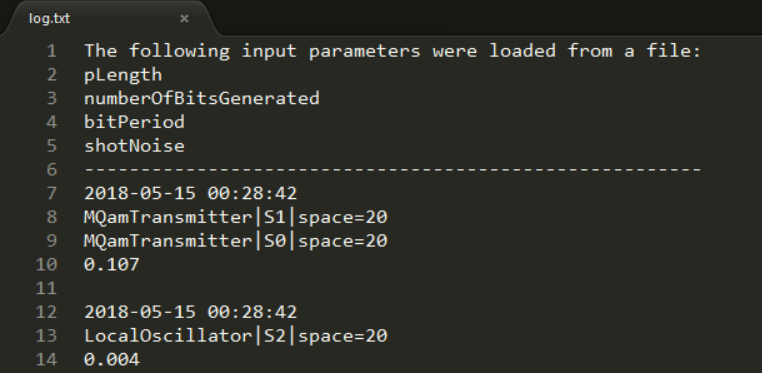
\includegraphics[width=.50\linewidth]{./chapter/simulator_structure/figures/logfile_input_parameters_changed}
\caption{Four input parameters where loaded from a file}
\label{fig:changedinputparameters}
\end{figure}

\subsection{Testing Log File}
In directory \textit{doc/tex/chapter/simulator\_structure/test\_log\_file/bpsk\_system/} there is a copy of the BPSK system. You may use it to test the Log File. The main method is located in file \textit{bpsk\_system\_sdf.cpp}

% bibliographic references for the section ----------------------------
\clearpage
\printbibliography[heading=subbibliography]
\end{refsection}
\addcontentsline{toc}{subsection}{Bibliography}
% ---------------------------------------------------------------------
\section{Input Parameters System}
\subsection{Introduction}
With the Input Parameters System (IPS) it is possible to read the input parameters from a file.

\subsubsection{Format Of The Input File}
In Figure \ref{fig:ipsfilecontent}, it is possible to observe the contents of the file \textbf{input\_parameters\_0.txt} used to load the values of some of the BPSK system's input parameters. The input file must respect the following properties:
\begin{enumerate}
\item Input parameter values can be changed by adding a line in the following format: \textbf{paramName=newValue}, where \textbf{paramName} is the name of the input parameter and \textbf{newValue} is the value to be assigned.
\item IPS supports scientific notation. This notation works for the lower case character \textbf{e} and the upper case character \textbf{E}.
\item If an input parameters is assigned the wrong type of value, method $\textbf{readSystemInputParameters()}$ will throw an exception.
\item Not all input parameters need to be changed.
\item The IPS supports comments in the form of the characters \textbf{//}. The comments will only be recognized if placed at the beginning of a line.
\end{enumerate}

\begin{figure}[H]
\centering
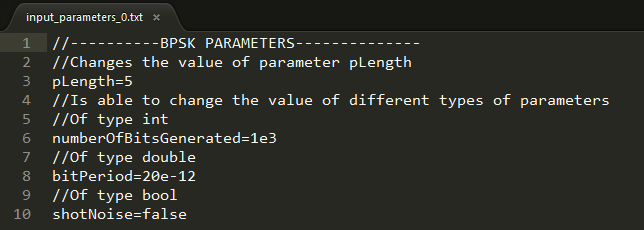
\includegraphics[width=0.8\linewidth]{./chapter/simulator_structure/figures/ips_input_file}
\caption{Content of file input\_parameters\_0.txt}
\label{fig:ipsfilecontent}
\end{figure}
\pagebreak
\subsubsection{Loading Input Parameters From A File}
Execute the following command in the Command Line:
\begin{itemize}
  \item[] \textbf{.\textbackslash{}some\_system.exe <input\_file\_path> <output\_directory>}
\end{itemize}
\
where \textbf{some\_system.exe} is the name of the executable generated after compiling the project, \textbf{<input\_file\_path>} is the path to the file containing the new input parameters; \textbf{<output\_directory>} is the directory where the output signals will be written into.

\subsection{How To Include The IPS In Your System}
In this illustrative example, the code of the BPSK System will be used. To implement the IPS the following requirements must be met:
\begin{enumerate}
\item Your system must include \textbf{netxpto\_20180418.h} or later.
\item A class that will contain the system input parameters must be created. This class must be a derived class of \textbf{SystemInputParameters}. In this case the created class is called \textbf{BPSKInputParameters}.
\item The created class must have 2 constructors. The implementation of these constructors is the same as \textbf{BPSKInputParameters}.
\begin{lstlisting}
BPSKInputParameters();
BPSKInputParameters(int argc, char*argv[]);
\end{lstlisting}
\item The created class must contain the method \textbf{initializeInputParameterMap()}. For every input parameter \textbf{addInputParameter(paramName,paramAddress)} must be called, where \textbf{paramName} is a string that represents the name of your input parameter and \textbf{paramAddress} is the address of your input parameter.
\begin{lstlisting}
void initializeInputParameterMap(){
	//Add parameters
}
\end{lstlisting}
\item All signals must be instantiated using the constructor that takes as argument, the file name and the folder name, according to the type of signal.
\begin{lstlisting}
Binary S0("S0.sgn", param.getOutputFolderName()) //S0 is a Binary signal
\end{lstlisting}
\item Method \textbf{main} must receive the following arguments.
\begin{lstlisting}
int main(int argc, char*argv[]){...}
\end{lstlisting}
\item The MainSystem must be instantiated using the following line of code. The \dots represent the list of blocks.
\begin{lstlisting}
System MainSystem{ vector<Block*> {...},param.getOutputFolderName(),param.getLoadedInputParameters()};
\end{lstlisting}
\end{enumerate}
\
The following code represents the input parameters class, \textbf{BPSKInputParameters}, and must be changed according to the system you are working on.
%%%%%%%%%%%%%%%%%%%%%%%%%%%CODE%%%%%%%%%%%%%%%%%%%%%%%%%%%%%%%%
\begin{lstlisting}
class BPSKInputParameters : public SystemInputParameters {
public:
	//INPUT PARAMETERS
	int numberOfBitsReceived{ -1 };
	int numberOfBitsGenerated{ 1000 };
	int samplesPerSymbol = 16;
    (...)

	/* Initializes default input parameters */
	BPSKInputParameters() : SystemInputParameters() {
		initializeInputParameterMap();
	}

	/* Initializes input parameters according to the program arguments */
    /* Usage: .\bpsk_system.exe <input_parameters.txt> <output_directory> */
	BPSKInputParameters(int argc, char*argv[]) : SystemInputParameters(argc,argv) {
		initializeInputParameterMap();
		readSystemInputParameters();
	}

	//Each parameter must be added to the parameter map by calling addInputParameter(string,param*)
	void initializeInputParameterMap(){
		addInputParameter("numberOfBitsReceived", &numberOfBitsReceived);
		addInputParameter("numberOfBitsGenerated", &numberOfBitsGenerated);
		addInputParameter("samplesPerSymbol", &samplesPerSymbol);
        (...)
	}
};
\end{lstlisting}
The method \textbf{main} should look similar to the following code.
\begin{lstlisting}
int main(int argc, char*argv[]){

    BPSKInputParameters param(argc, argv);

    //Signal Declaration and Initialization
    Binary S0("S0.sgn", param.getOutputFolderName());
	S0.setBufferLength(param.bufferLength);

	OpticalSignal S1("S1.sgn", param.getOutputFolderName());
	S1.setBufferLength(param.bufferLength);
    (...)

    //System Declaration and Initialization
	System MainSystem{ vector<Block*> { &B1, &B2, &B3, &B4, &B5, &B6, &B7, &B8},param.getOutputFolderName(),param.getLoadedInputParameters()};

    //System Run
	MainSystem.run();

	return 0;
}
\end{lstlisting}
%%%%%%%%%%%%%%%%%%%%%%%%%%%%%%%%%%%%%%%%%%%%%%%%%%%%%%%%%%%%%%%%%%%%%%
\pagebreak
The class \textbf{SystemInputParameters}, has the following constructors and methods available:
\begin{table}[H]
\centering
\begin{tabulary}{1.0\textwidth}{|p{5cm}|p{10cm}|}
\hline
\multicolumn{2}{|c|}{ \textbf{SystemInputParameters - Constructors} } \\
\hline
\textbf{Constructors}                   & \textbf{Comments} \\ \hline
SystemInputParameters()                        & Creates an object of SystemInputParameters with the default input parameters' values\\ \hline
SystemInputParameters(int argc, char*argv[])   & Creates an object of SystemInputParameters and loads the values according to the program arguments passed in the command line\\ \hline
\end{tabulary}
\end{table}

\begin{table}[H]
\centering
\begin{tabulary}{1.0\textwidth}{|p{9cm}|p{1cm}|p{5cm}|}
\hline
\multicolumn{3}{|c|}{ \textbf{SystemInputParameters - Methods} } \\
\hline
\textbf{Method}                                      & \textbf{Type} & \textbf{Comments} \\ \hline
addInputParameter(string name, int* variable)        & void          & Adds an input parameter whose value is of type int\\ \hline
addInputParameter(string name, double* variable)     & void	         & Adds an input parameter whose value is of type double\\ \hline
addInputParameter(string name, bool* variable)       & void	         & Adds an input parameter whose value is of type bool\\ \hline
readSystemInputParameters()                          & void	         & Reads the input parameters from a file.\\ \hline
\end{tabulary}
\end{table}

\cleardoublepage 
\include{chapter/development_cycle}
\include{chapter/visualizer}

% ------------------------------------------------------------------------
\chapter{Case Studies}

\ifdefined\qpsk         \input{./sdf/qpsk_transmitter/qpsk_transmitter} \fi
\ifdefined\optical      \input{./sdf/optical_detection/optical_detection} \fi
\ifdefined\bpsk         \input{./sdf/bpsk_system/bpsk_system} \fi
\ifdefined\m            \clearpage
\section{M-QAM Transmission System}

\begin{tcolorbox}	
	\begin{tabular}{p{2.75cm} p{0.2cm} p{10.5cm}} 	
		\textbf{Student Name}  &:& Ana Luisa Carvalho (2017/04/01 - 2017/12/31) \\
		\textbf{Goal}          &:& M-QAM system implementation with BER measurement and comparison with theoritical values.\\
		\textbf{Directory} &:& sdf/m\_qam\_system
	\end{tabular}
\end{tcolorbox}

The goal of this project is to simulate a Quadrature Amplitude Modulation transmission system with M points in the constellation diagram (M-QAM) and to perform a Bit Error Rate (BER) measurement that can be compared with theoretical values. 

M-QAM systems can encode $\log_2 M$ bits per symbol which means they can transmit higher data rates keeping the same bandwidth when compared, for example, to PSK systems. However, because the states are closer together, these systems are more susceptible to noise.

The Bit Error Rate (BER) is a measurement of how a bit stream is altered by a transmission system due to noise (among other factors). To study this effect we introduced Additive White Gaussian Noise (AWGN) to model thermal noise at the receiver. 

For $M=4$ the M-QAM system reduces to a Quadrature Phase Shift Keying system (QPSK) system that uses four equispaced points in the constellation diagram (see figure \ref{fig:const}). 

\begin{figure}[h]
	\centering
	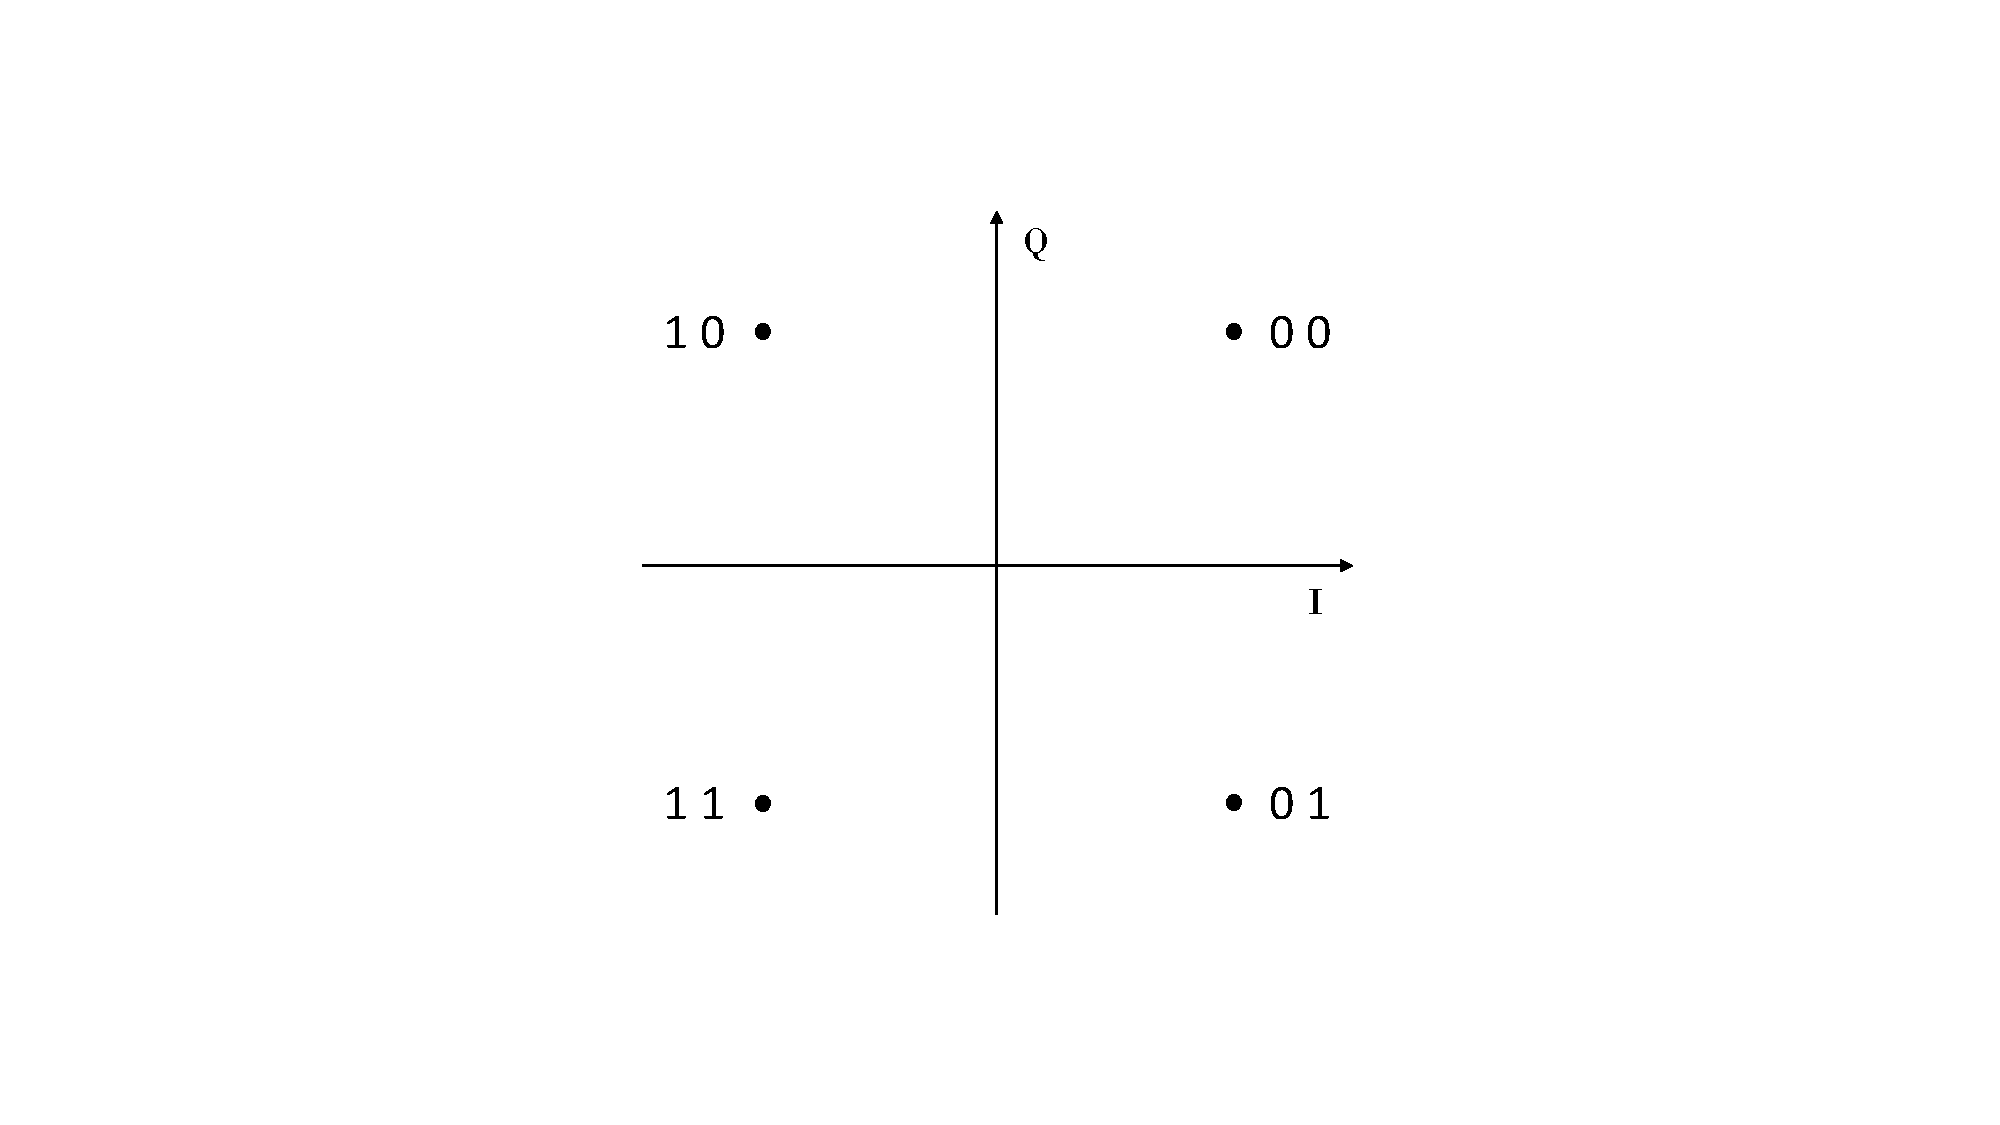
\includegraphics[clip, trim=3cm 3cm 3cm 3cm, width=\textwidth]{./sdf/m_qam_system/figures/MQAM_constellation.pdf}
	\caption{4-QAM constellation points.}
	\label{fig:const}
\end{figure}

%M can take several values: $2, 4, 16, 32, ...$. The first two correspond to BPSK and QPSK modulation, respectively.

\subsection{Theoretical Analysis }

M-QAM is a modulation scheme that takes advantage of two carriers (usually sinusoidal waves) with a phase difference of $\frac{\pi}{2}$. The resultant output consists of a signal with both amplitude and phase variations. The two carriers, refered to as I (In-phase) and Q (Quadrature), can be represented as 

\begin{align}
	I=A\cos(\phi) \\
	Q=A\sin(\phi)
\end{align}
which means that any sinusoidal wave can be decomposed in its I and Q components:

\begin{align}
	A\cos(\omega~t+\phi)&=A\left(\cos(\omega~t)\cos(\phi)-\sin(\omega~t)\sin(\phi)\right) \\
	&=I\cos(\omega~t)-Q\sin(\omega~t),
\end{align} 
where we have used the expression for the cossine of a sum and the definitions of I and Q.

%When demodulating a signal it is necessary to associate the received signal to the corresponding signal. The existence of noise in the channel means that we can only compute the probability that a given signal corresponds to a certain carrier and that's why we need to define the BER. Using
%
%\begin{equation}
%P_i f(s|c_i)>P_j f(s|c_j), \qquad i\neq j
%\end{equation}
%where $f(s|c_i)$ stands for the probability of detecting the signal $s$ given that $c_i$ was emmited. This inequallity can be rewritten in the following way
%
%\begin{equation}
%P(c_i|s)>P(c_j|s)
%\end{equation}
%where $P(c_i|s)$ and $P(c_j|s)$ are called \textit{a posteriori} probabilities and represent the probability that $c_i$ or $c_j$ were transmitted given that $s$ was received. In terms of the systems this simply means that we should select the signal most likely to have been transmitted.
%
%In the case of additive white gaussian noise the $f$ function is simply given by
%
%\begin{equation}
%f(s|c_i)=\frac{e^{-x^2/n_0}}{(\pi n_0)^{N/2}}
%\end{equation}
%where $x$ is the Euclidean distance in the I-Q plane between the signal received and carrier i and $N$ is the number of noise samples.
%
%When using 4-QAM modulation all points are at an equal distance from the origin (in the I-Q plane) so they all have the same energy given by
%
%\begin{equation}
%E=\frac{d^2}{2}
%\end{equation}
%where $d$ is the side of the square formed bye the constellation points.
%
%The probability that a given signal is identified correctly is given by
%
%\begin{equation}
%P_c=r^2
%\end{equation}
%where $n_0/2$ is the noise variance for AWGN and
%
%\begin{equation}
%r=\int_{-d/2}^{\infty}\frac{e^{-x^2/n_0}}{\sqrt{\pi n_0}} dx.
%\end{equation}
%
%The error probability, $P_e$, given by $1-P_c$ is given by
%
%\begin{equation}
%P_e=\erfc \sqrt{\frac{E}{2 n_0}}.
%\end{equation}

The probability of symbol error, $P_s$, in coherent M-PSK demodulation with AWGN is given by 

\begin{equation}
	P_s=2~Q\left(\sqrt{2~\log_2 M \left(\frac{E_b}{n_0}\right)\sin^2\frac{\pi}{M}}\right)
\end{equation}
where $E_b$ is the energy of one bit, $n_0$ is the noise power and the function $Q$ is defined as
\begin{equation}
	Q(x)=\frac{1}{2} erfc\left(\frac{x}{\sqrt{2}}\right).
	\label{eq:Ps}
\end{equation}

The probability of bit errors, $P_b$ is related to $P_s$ by
\begin{equation}
	P_b=\frac{1}{\log_2 M}P_s.
	\label{eq:Pb}
\end{equation} 

For QPSK we get, using $M=4$ in equations \ref{eq:Ps} and \ref{eq:Pb},
\begin{equation}
	P_b=\frac{1}{2} erfc\left(\sqrt{\frac{2~E_b}{n_0}}\right).
\end{equation}

This function is plotted in figure \ref{fig:QPSK_th_curve} for $n_0=10^{-6}$.

\begin{figure}[h]
		\centering
		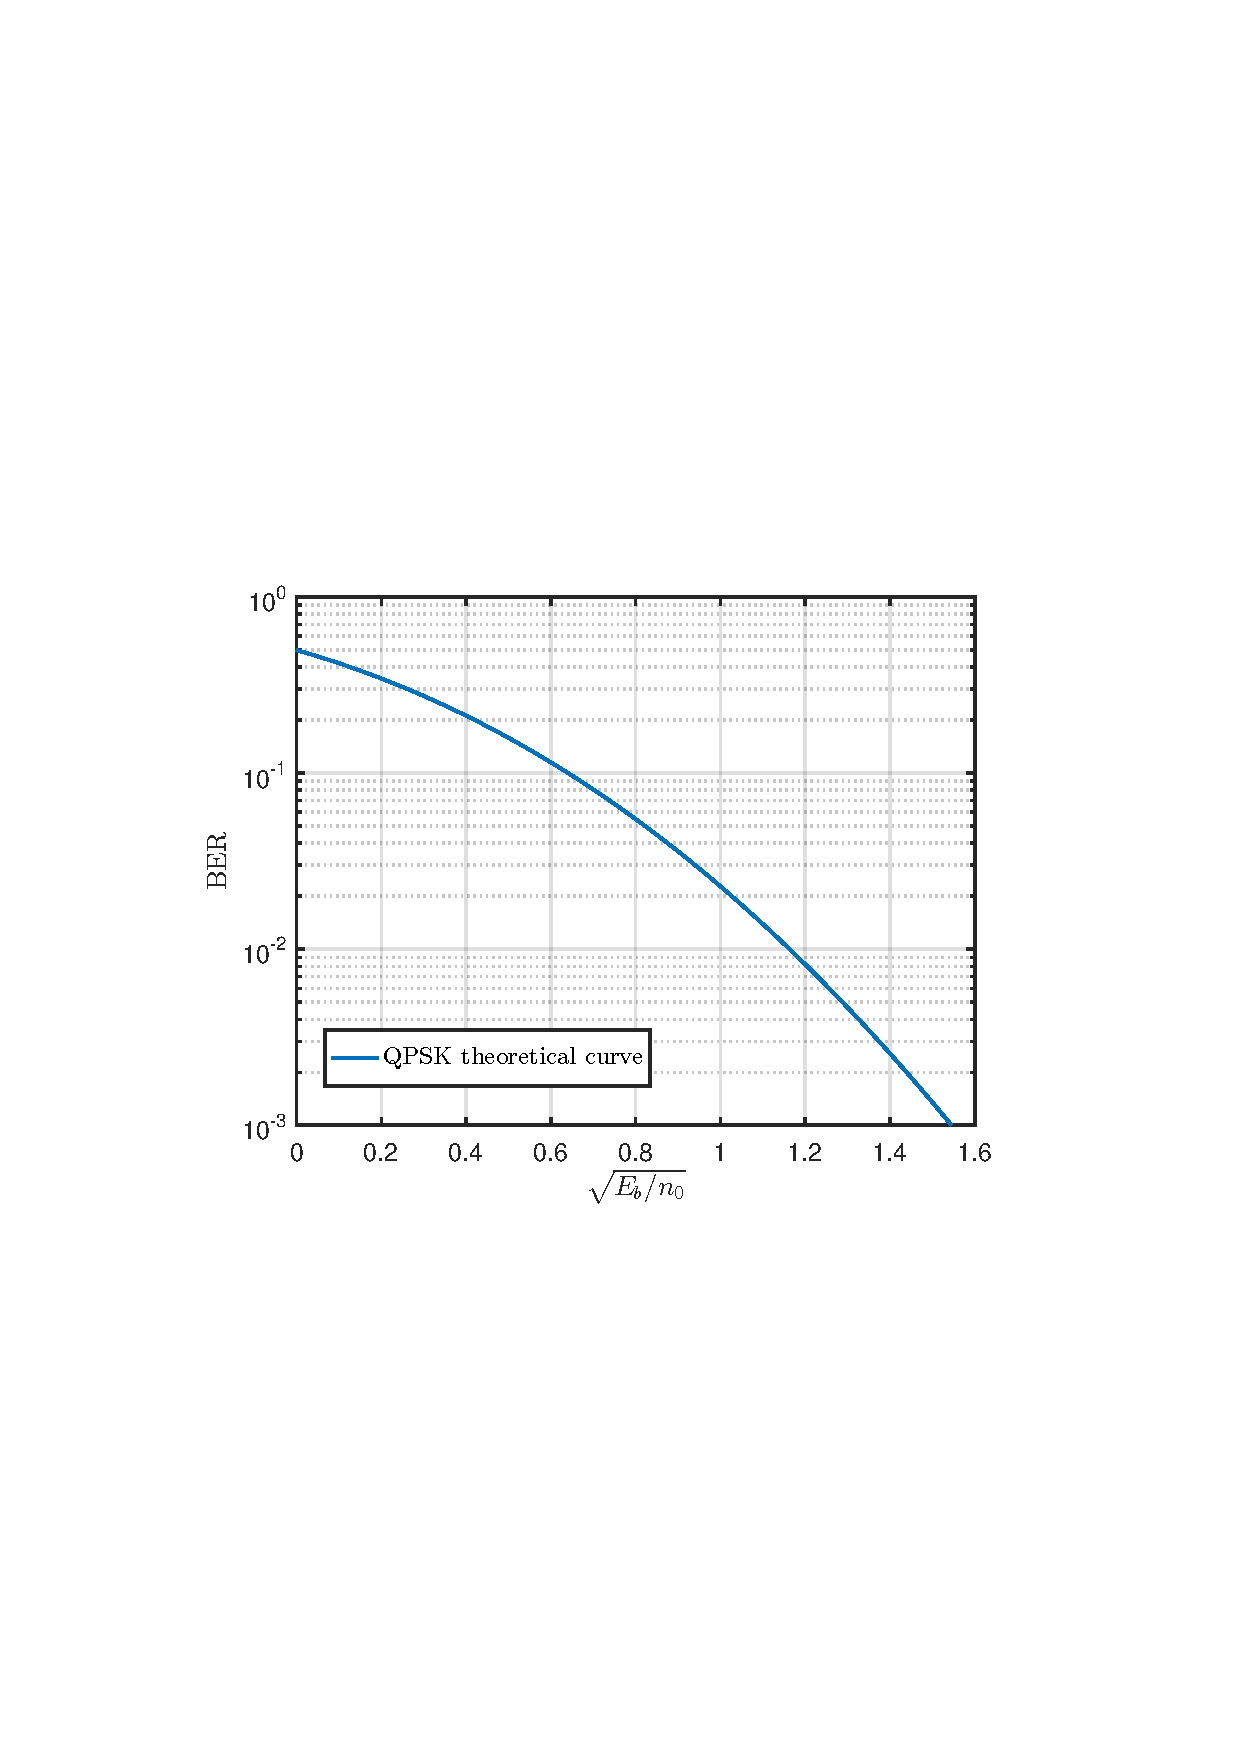
\includegraphics[clip, trim=0.5cm 9cm 0.5cm 9cm, width=\textwidth]{./sdf/m_qam_system/figures/BER_QPSK_theory_Eb_n0.pdf}
		\caption{QPSK theoretical BER values as a function of the output optical power in dBm.}
		\label{fig:QPSK_th_curve}
\end{figure}

\pagebreak
\subsection{Simulation Analysis}

The system to be simulated is composed of four blocks: a M-QAM transmitter, a M-QAM receiver, a sink and a block that performs a Bit Error Rate (BER) measurement. This system is a complex block of code that simulates the modulation, transmission and demodulation of an optical signal using M-QAM modulation. The schematic representation of the
system is presented in figure \ref{MQAM_system_block_diagram}. 

\begin{figure}[!b]
	\centering
	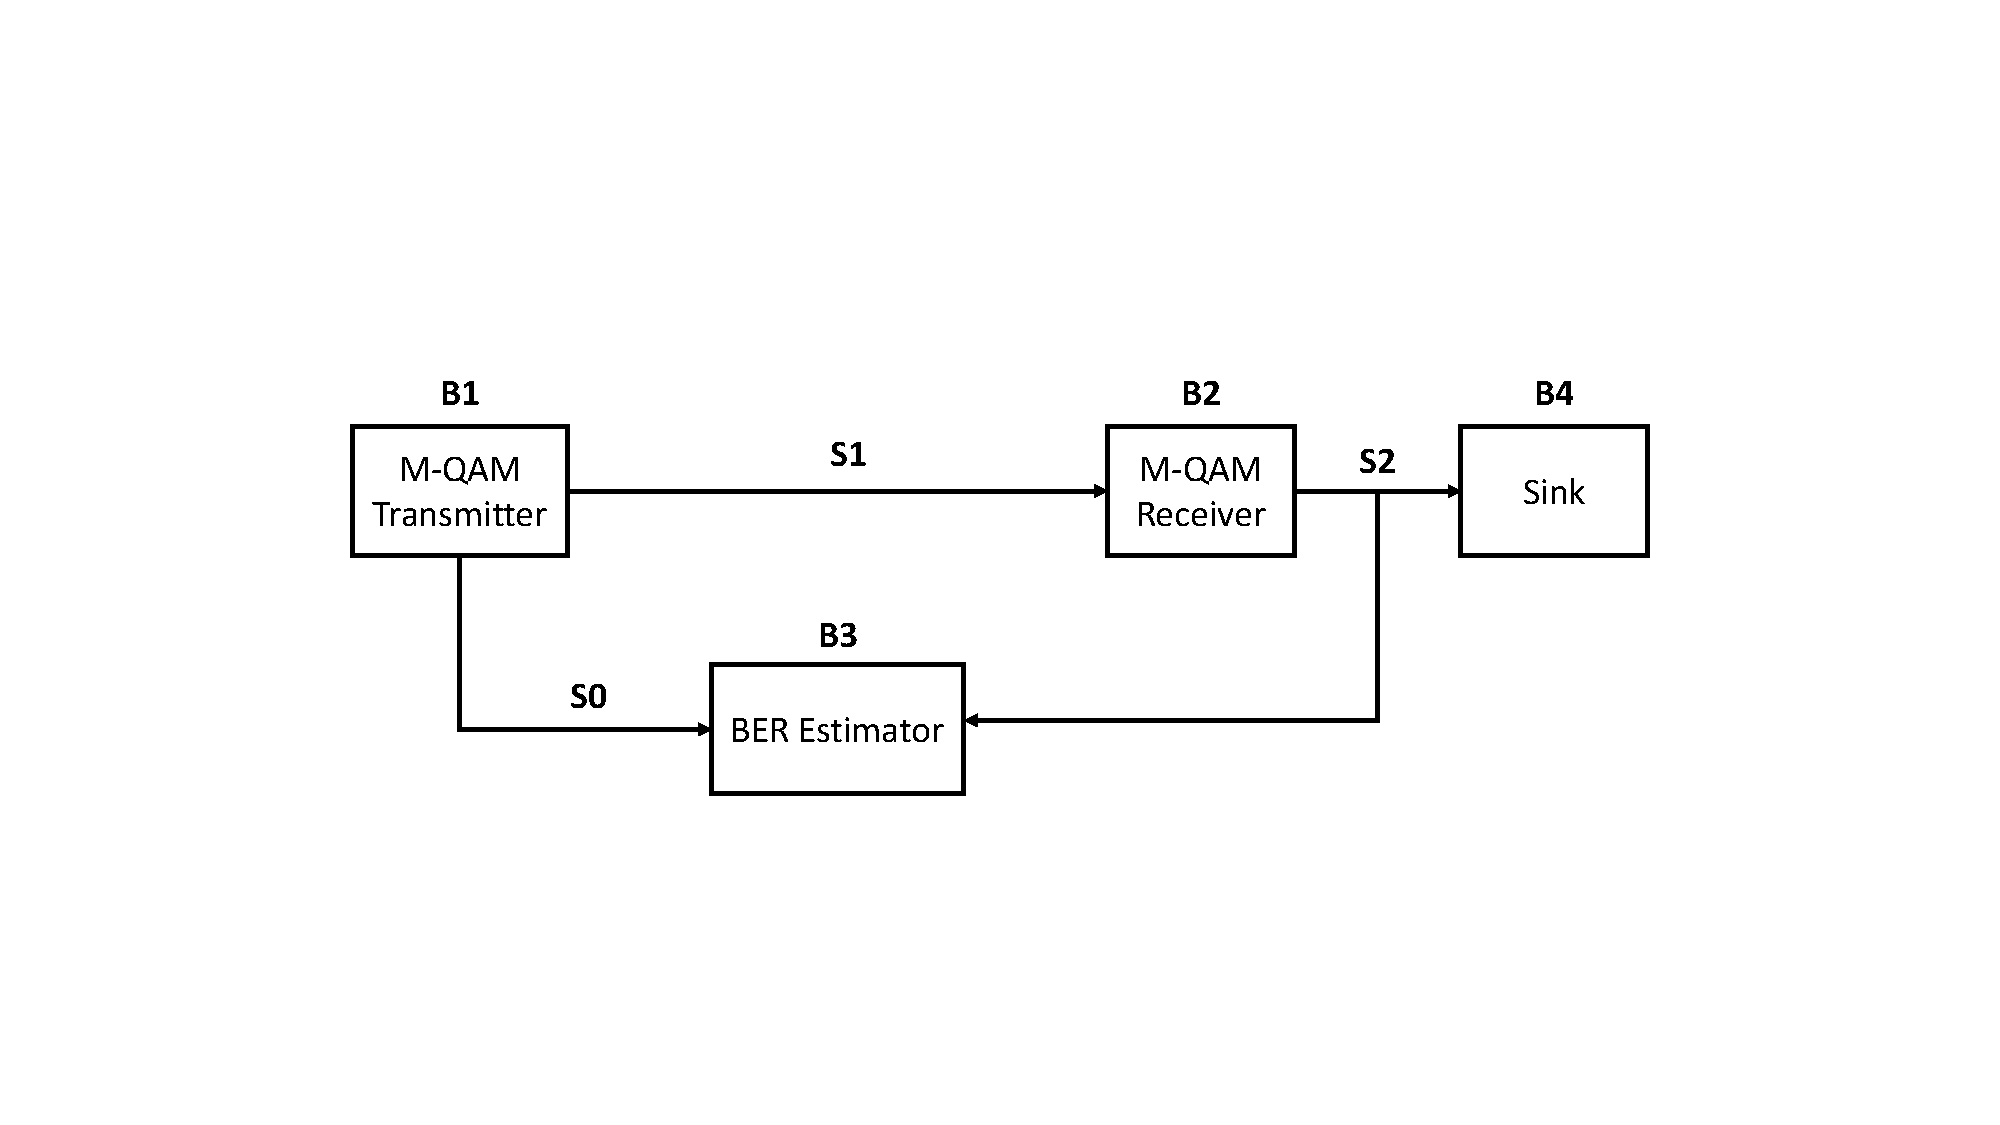
\includegraphics[trim={4cm 4cm 4cm 6cm},clip,width=\textwidth]{./sdf/m_qam_system/figures/MQAM_system_block_diagram.pdf}
	\caption{Schematic representation of the M-QAM system.}\label{MQAM_system_block_diagram}
\end{figure}

%The M-QAM transmission system is a complex block of code that simulates the modulation, transmission and demodulation of an optical signal using M-QAM modulation.

\paragraph{Current state:} The system currently being implement is a QPSK system (M=4).

\paragraph{Future work:} Extend this block to include other values of M.

\subsection*{Functional description}

A complete description of the M-QAM transmitter and M-QAM homodyne receiver blocks can be found in the \textit{Library} chapter of this document as well as a detailed description of the independent blocks that compose these blocks.

The M-QAM transmitter generates one or two optical signals by enconding a binary string using M-QAM modulation. It also outputs a binary signal that is used to perform the BER measurement.

The M-QAM homodyne receiver accepts one input optical signal and outputs
a binary signal. It performs the M-QAM demodulation of the input signal by combining the optical signal with a local oscillator.

The demodulated optical signal is compared to the one produced by the transmitter in order to estimate the Bit Error Rate (BER).

\subsection*{Input Parameters}

The system accepts several input parameters that can be defined by the user. These are described in table \ref{table:in_par}.

\begin{table}[h]
	\centering
	\caption{Input parameters}
	\begin{tabular}{|c|c|p{70mm}|ccp{70mm}}
		\cline{1-3}
		\textbf{Parameter} & \textbf{Type} & \textbf{Description} &    \\ \cline{1-3}
		%numberOfBitsGenerated & t\_integer & Determines the number of bits to be generated by the binary source  &    \\ \cline{1-3}
		%samplesPerSymbol & t\_integer & Number of samples per symbol &    \\ \cline{1-3}
		%prbsPatternLength & int & Determines the length of the pseudorandom sequence pattern (used only when the binary source is operated in \textit{PseudoRandom} mode) &    \\ \cline{1-3}
		%bitPeriod & t\_real & Temporal interval occupied by one bit &    \\ \cline{1-3}
		%rollOffFactor & t\_real & Parameter of the raised cosine filter &    \\ \cline{1-3}
		signalOutputPower\_dBm & t\_real & Determines the power of the output optical signal in dBm &  \\ \cline{1-3}
		numberOfBitsReceived & int &   Determines when the simulation should stop. If $-1$ then it only stops when there is no more bits to be sent&   \\ \cline{1-3}
		iqAmplitudeValues & vector<t\_iqValues> & Determines the constellation used to encode the signal in IQ space &    \\ \cline{1-3}
		%symbolPeriod & double & Given by bitPeriod/samplesPerSymbol &    \\ \cline{1-3}
		%localOscillatorPower\_dBm & t\_real & Power of the local oscillator &    \\ \cline{1-3}
		%responsivity & t\_real & Responsivity of the photodiodes (1 corresponds to having all optical power transformed into electrical current) &    \\ \cline{1-3}
		%amplification & t\_real & Amplification provided by the ideal amplifier &    \\ \cline{1-3}
		%noiseAmplitude & t\_real & Amplitude of the white noise &    \\ \cline{1-3}
		%samplesToSkip & t\_integer & Number of samples to be skipped by the \textit{sampler} block &    \\ \cline{1-3}
		%confidence & t\_real & Determines the confidence limits for the BER estimation &    \\ \cline{1-3}
		%midReportSize & t\_integer &  &    \\ \cline{1-3}
		%bufferLength & t\_integer & Corresponds to the number of samples that can be processed in each run of the system &    \\ \cline{1-3}
	\end{tabular}
	\label{table:in_par}
\end{table}

\subsection*{Required Files}

The required header and source files needed to run this system are summarized in table \ref{table:files}.

\begin{table}[]
	\centering
	\caption{Main system files}
	\begin{tabular}{|c|c|p{35mm}|c|ccc}
		\cline{1-4}
		\textbf{Source file} & \textbf{Header file}  &  \textbf{System blocks} & \textbf{Status} & \\ \cline{1-4}
		m\_qam\_system\_sdf.cpp & --- & Main &\checkmark & \\ \cline{1-4}
		m\_qam\_transmitter.cpp & m\_qam\_transmitter.h & M-QAM Transmitter & \checkmark &  \\ \cline{1-4}
		m\_qam\_homodyne\_receiver.cpp & homodyne\_receiver.h & M-QAM Receiver & \checkmark &  \\ \cline{1-4}
		sink.cpp & sink.h & Sink & \checkmark & \\ \cline{1-4}
		bit\_error\_rate.cpp & bit\_error\_rate.h & BER Estimator & \checkmark &\\ \cline{1-4}
		add.cpp & add.h & M-QAM transmitter & \checkmark & \\ \cline{1-4}
		binary\_source.cpp & binary\_source.h & M-QAM Transmitter & \checkmark & \\ \cline{1-4}
		discrete\_to\_continuous\_time.cpp & discrete\_to\_continuous\_time.h & M-QAM Transmitter & \checkmark & \\ \cline{1-4}
		ideal\_amplifier.cpp & ideal\_amplifier.h & M-QAM Receiver & \checkmark & \\ \cline{1-4}
		iq\_modulator.cpp & iq\_modulator.h & M-QAM Transmitter & \checkmark & \\ \cline{1-4}
		local\_oscillator.cpp & local\_oscillator.h & M-QAM Receiver & \checkmark & \\ \cline{1-4}
		m\_qam\_mapper.cpp & m\_qam\_mapper.h & M-QAM Transmitter & \checkmark & \\ \cline{1-4}
		netxpto.cpp & netxpto.h & All & \checkmark & \\ \cline{1-4}
		optical\_hybrid.cpp & optical\_hybrid.h & M-QAM Receiver & \checkmark & \\ \cline{1-4}
		photodiode\_old.cpp & photodiode\_old.h & M-QAM Receiver & \checkmark & \\ \cline{1-4}
		pulse\_shaper.cpp & pulse\_shaper.h & M-QAM Transmitter \newline M-QAM receiver & \checkmark & \\ \cline{1-4}
		sampler\_20171119.cpp & sampler\_20171119.h & M-QAM Receiver & \checkmark & \\ \cline{1-4}
		sink.cpp & sink.h & Sink & \checkmark & \\ \cline{1-4}
		super\_block\_interface.cpp & super\_block\_interface.h & ? & \checkmark & \\ \cline{1-4}
		white\_noise.cpp & white\_noise.h & M-QAM Receiver & \checkmark & \\ \cline{1-4}
	\end{tabular}
	\label{table:files}
\end{table}

%\begin{table}
% 	\centering
% 	\caption{Required files}
% 	\begin{tabular}{|c|c|p{40mm}|c|ccp{40mm}c}
% 		\cline{1-4}
% 		\textbf{Header file} & \textbf{Source file} & \textbf{Description} &  \textbf{Status} & \\ \cline{1-4}
% 		add.h & add.cpp & Adds two signals.  & \checkmark &   \\ \cline{1-4}
% 		binary\_source.h & binary\_source.cpp & Produces a binary sequence. & \checkmark & \\ \cline{1-4}
% 		bit\_error\_rate.h & bit\_error\_rate.cpp & Computes the BER and writes it to a text file. & \checkmark & \\ \cline{1-4}
% 		discrete\_to\_continuous\_time.h & discrete\_to\_continuous\_time.cpp & Converts a signal from discrete in time to continuous in time. & \checkmark & \\ \cline{1-4}
% 		homodyne\_receiver.h & m\_qam\_homodyne\_receiver.cpp & & \\ \cline{1-4}
% 		ideal\_amplifier.h & ideal\_amplifier.cpp & Amplifies the signal. & \checkmark & \\ \cline{1-4}
% 		iq\_modulator.h & iq\_modulator.cpp & Divides the signal in its quadrature and in phase components & \checkmark &\\ \cline{1-4}
% 		local\_oscillator.h & local\_oscillator.cpp & & & \checkmark &\\ \cline{1-4}
% 		m\_qam\_mapper.h & m\_qam\_mapper.cpp & Maps the signal using the defined constellation & \checkmark & \\ \cline{1-4}
% 		m\_qam\_transmitter.h & m\_qam\_transmitter.cpp & & \checkmark & \\ \cline{1-4}
% 		netxpto.h & netxpto.cpp & General class that contains definition from signals and buffers. & \checkmark &\\ \cline{1-4}
% 		optical\_hybrid.h & optical\_hybrid.cpp & Implements an optical hybrid. & \checkmark & \\ \cline{1-4}
% 		photodiode\_old.h & photodiode\_old.cpp & Pair of photodiodes and current subtraction. & \checkmark & \\ \cline{1-4}
% 		pulse\_shaper.h & pulse\_shaper.cpp & Electrical filter. & \checkmark &\\ \cline{1-4}
% 		sampler\_20171119.h & sampler\_20171119.cpp & Samples the signal. & \checkmark &\\ \cline{1-4}
% 		sink.h & sink.cpp & Deletes signal. & \checkmark & \\ \cline{1-4}
% 		super\_block\_interface.h & super\_block\_interface.cpp & & \checkmark &\\ \cline{1-4}
% 		white\_noise.h & white\_noise.cpp & Generates white gaussian noise. & \checkmark &\\ \cline{1-4}  
% 	\end{tabular}
% 	\label{table:files}
%\end{table}

\pagebreak
\subsection*{Simulation results}

The parameters used to produce the results presented in this section are summarized in table \ref{table:par}.

\begin{table}[]
	\centering
	\caption{Values of the simulation parameters}
	\begin{tabular}{|c|c|cc}
		\cline{1-2}
		\textbf{Parameter} & \textbf{Value} & \\ \cline{1-2}
		numberOfBitsGenerated & $4000$ & \\ \cline{1-2}
		samplesPerSymbol & $16$ & \\ \cline{1-2}
		bitPeriod & $20$~ps & \\ \cline{1-2}
		rollOfFactor & $0.9$ & \\ \cline{1-2}
		prbsPatternLength & $7$ & \\ \cline{1-2}
		symbolPeriod & $1.25$~ps & \\ \cline{1-2}
		localOscillatorPower\_dBm & $0$ & \\ \cline{1-2}
		localOscillatorPhase & $0$ & \\ \cline{1-2}
		responsivity & $1$ & \\ \cline{1-2}
		amplification & $10^3$ & \\ \cline{1-2}
		noiseAmplitude & $10^{-6}$ & \\ \cline{1-2}
		samplesToSkip & $256$ & \\ \cline{1-2}
		confidence & $0.95$ & \\ \cline{1-2}
		midReportSize & $0$ & \\ \cline{1-2}
		bufferLength & $512$ & \\ \cline{1-2}
	\end{tabular}
	\label{table:par}
\end{table}

We show the eye diagrams for the signals HMD14 and HMD15 (see figure \ref{fig:MQAM_receiver}) for $\sqrt{\frac{E_b}{n_0}}=10^{-8},1,10^6$. These correspond to figures \ref{fig:eye_diagram_140}, \ref{fig:eye_diagram_60}, \ref{fig:eye_diagram_0}, respectively. We also show, in figure \ref{fig:ber_pseudorandom_sim}, the plot of the BER as a function of $\sqrt{\frac{E_b}{n_0}}$.

\begin{figure}[]
	\centering
	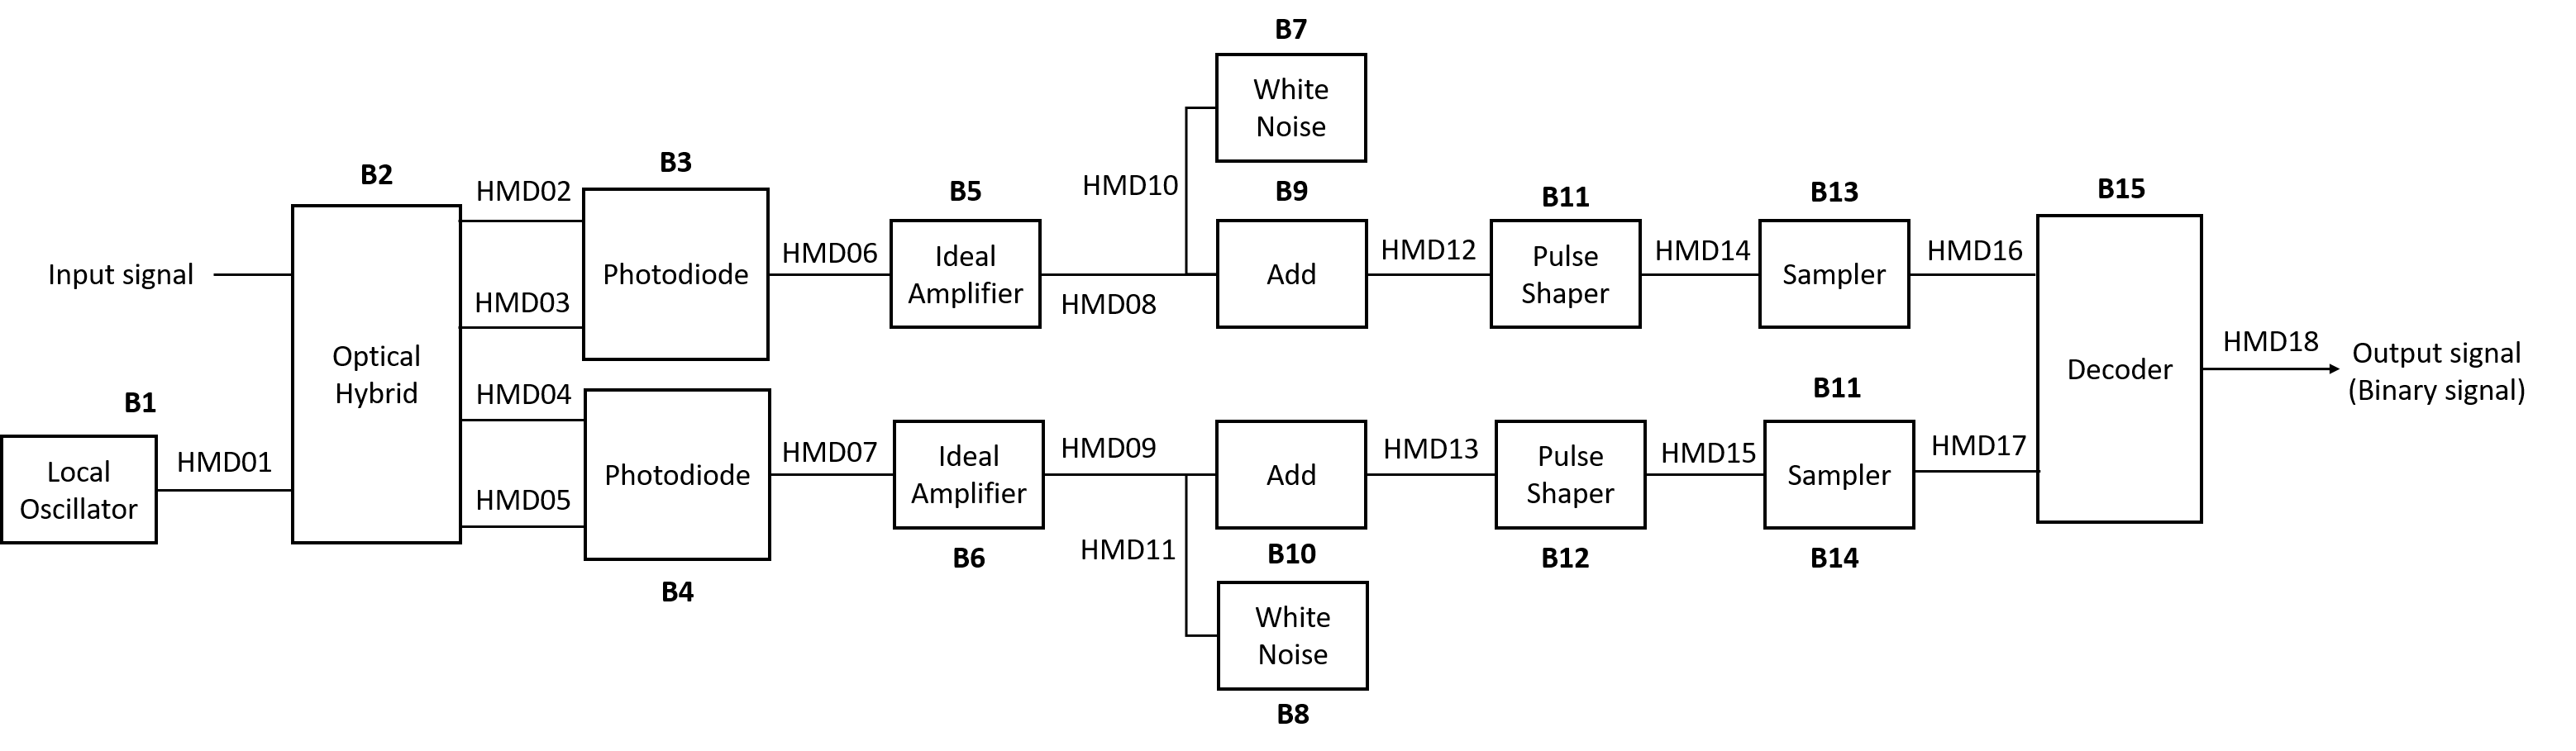
\includegraphics[width=1.1\textwidth]{./lib/homodyne_receiver/figures/MQAM_receiver_block_diagram.png}
	\caption{M-QAM receiver schematic representation}
	\label{fig:MQAM_receiver}
\end{figure}

\begin{figure}
	\centering
	\begin{subfigure}{.5\textwidth}
		\centering
		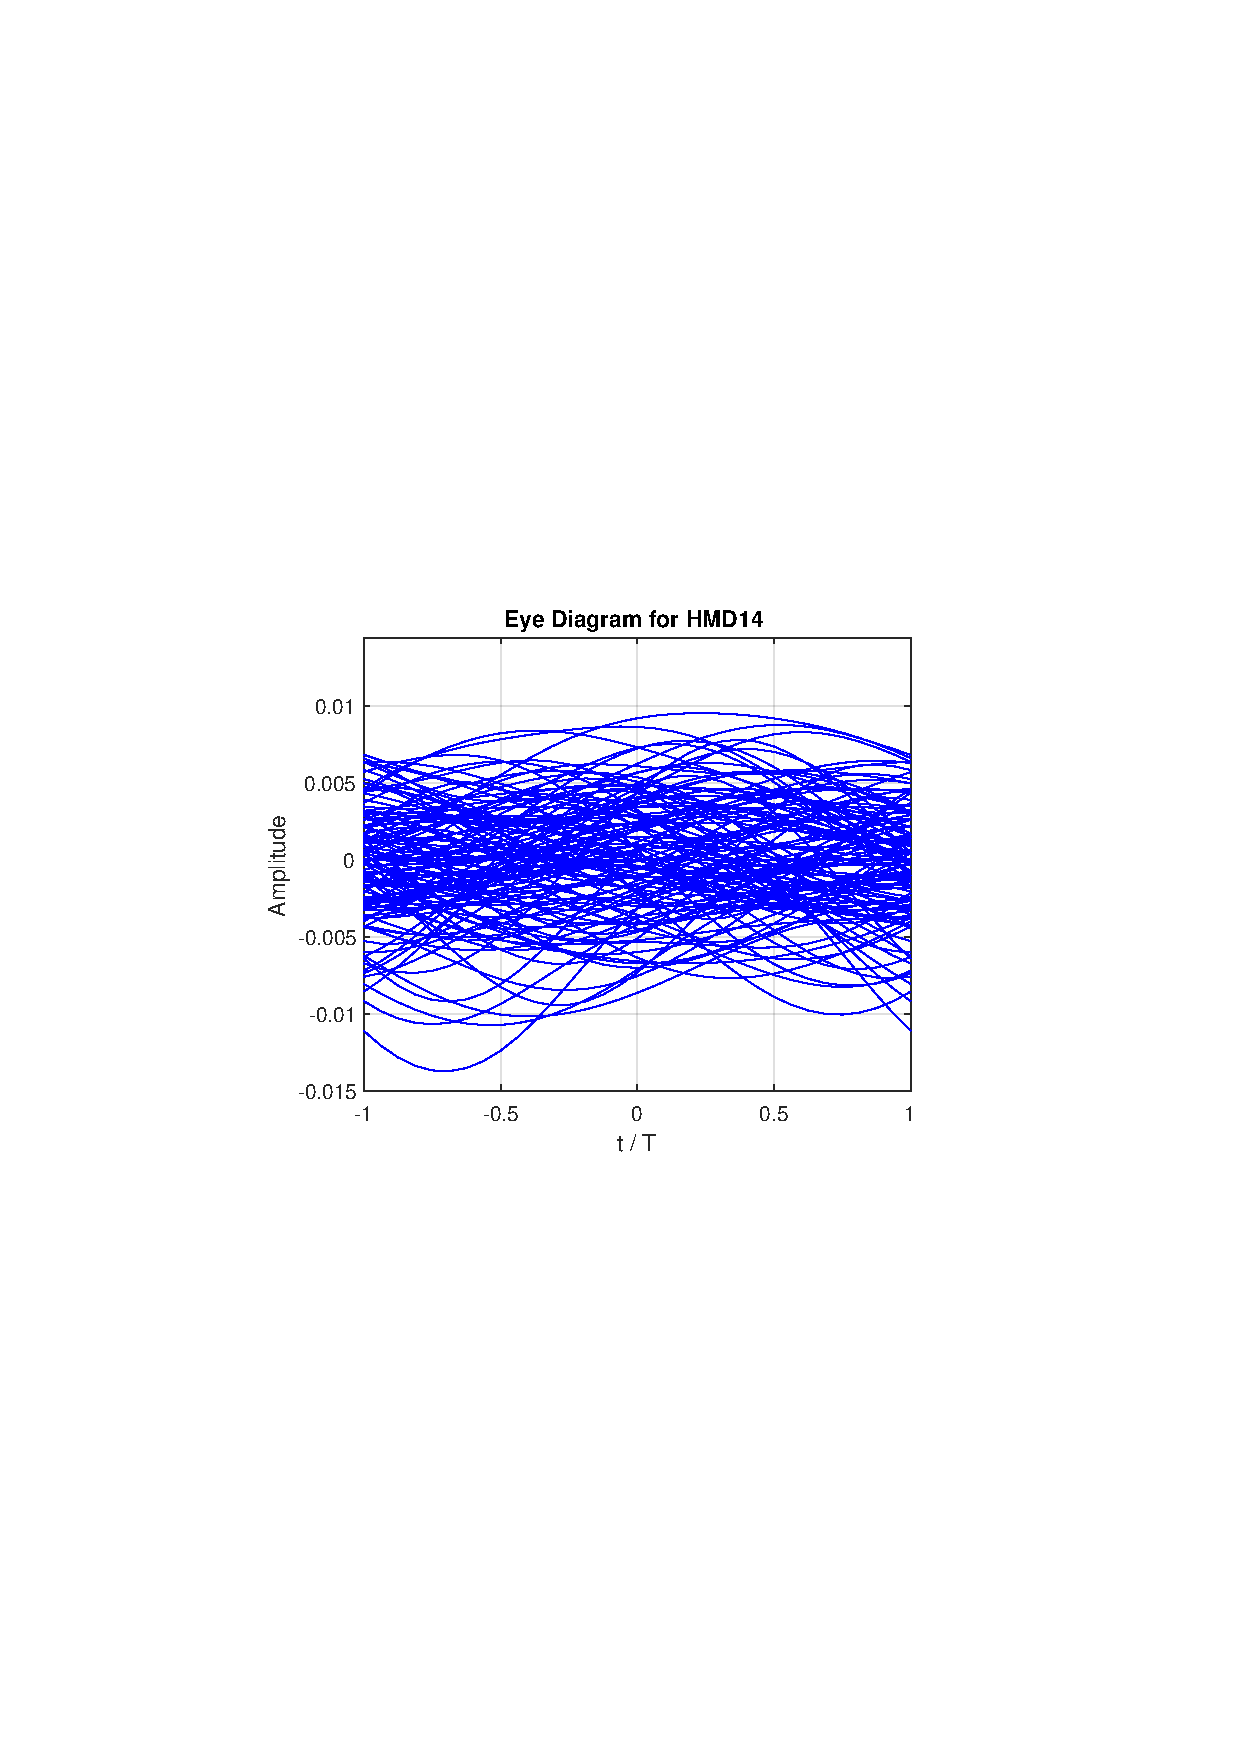
\includegraphics[clip, trim=5cm 10cm 5cm 10cm, width=\textwidth]{./sdf/m_qam_system/figures/HMD14_eye_diagram_140.pdf}
	\end{subfigure}%
	\begin{subfigure}{.5\textwidth}
		\centering
		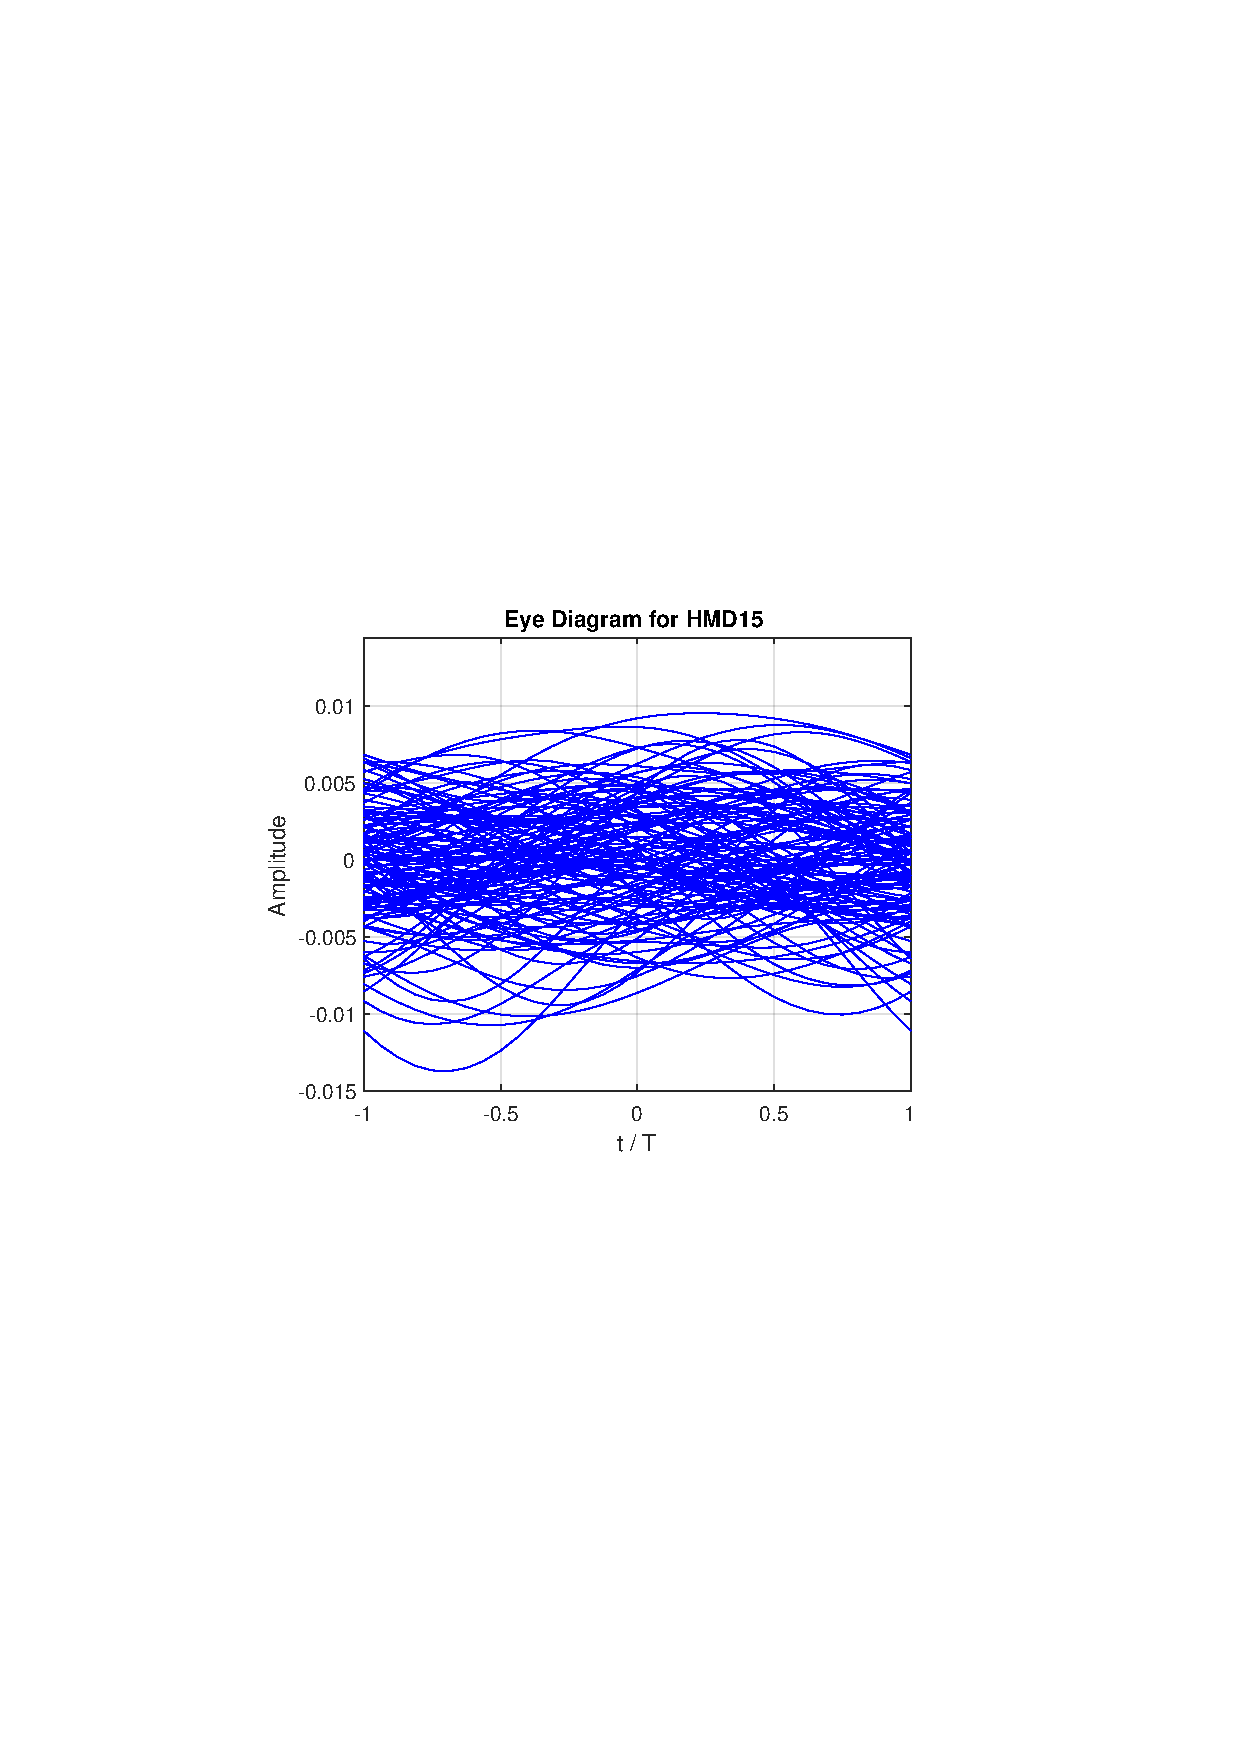
\includegraphics[clip, trim=5cm 10cm 5cm 10cm, width=\textwidth]{./sdf/m_qam_system/figures/HMD15_eye_diagram_140.pdf}
	\end{subfigure}
	\caption{Eye diagrams for the signals HMD14 (left) and HMD15 (right) for signalOutputPower\_dBm $=-140$. This corresponds to $\sqrt{\frac{E_b}{n_0}}=10^{-8}$.}
	\label{fig:eye_diagram_140}
\end{figure}

\begin{figure}
	\centering
	\begin{subfigure}{.5\textwidth}
		\centering
		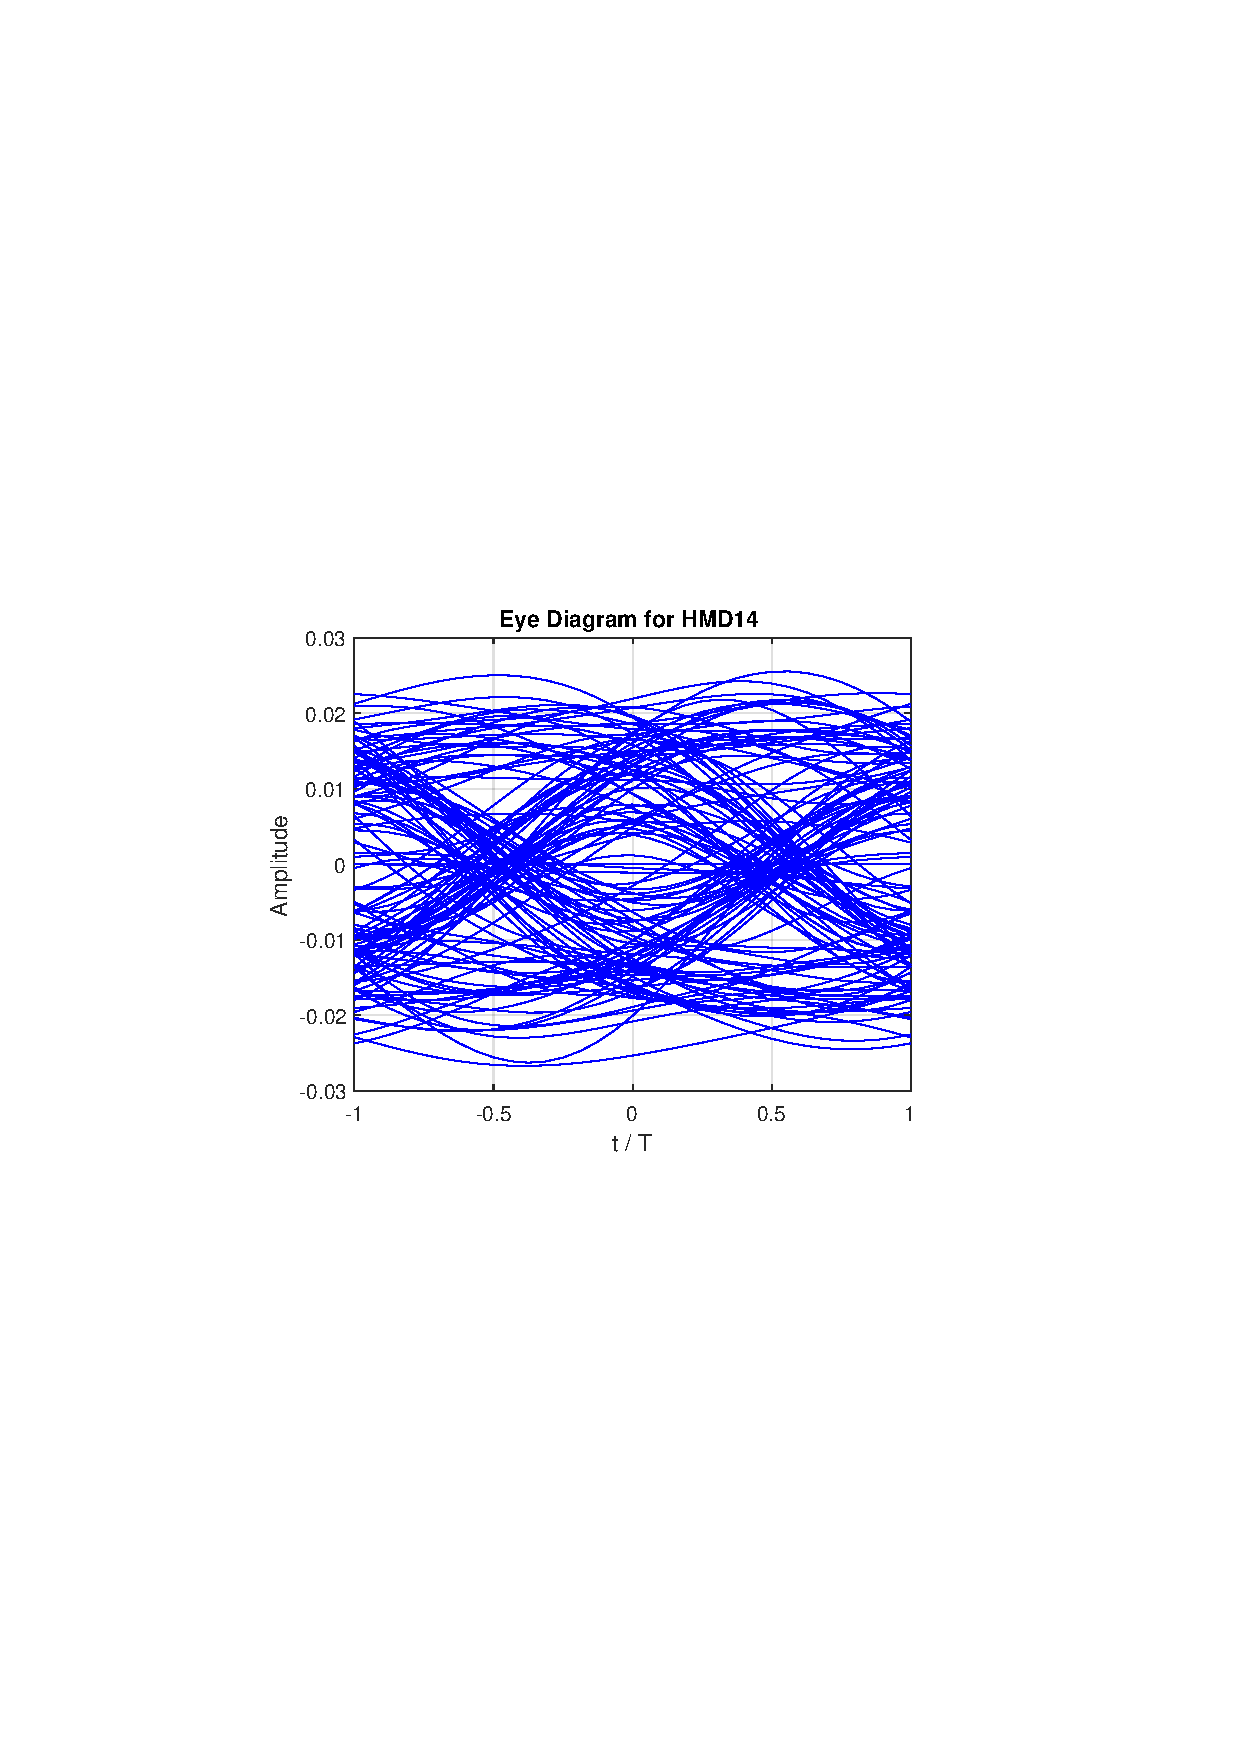
\includegraphics[clip, trim=5cm 10cm 5cm 10cm, width=\textwidth]{./sdf/m_qam_system/figures/HMD14_eye_diagram_60.pdf}
	\end{subfigure}%
	\begin{subfigure}{.5\textwidth}
		\centering
		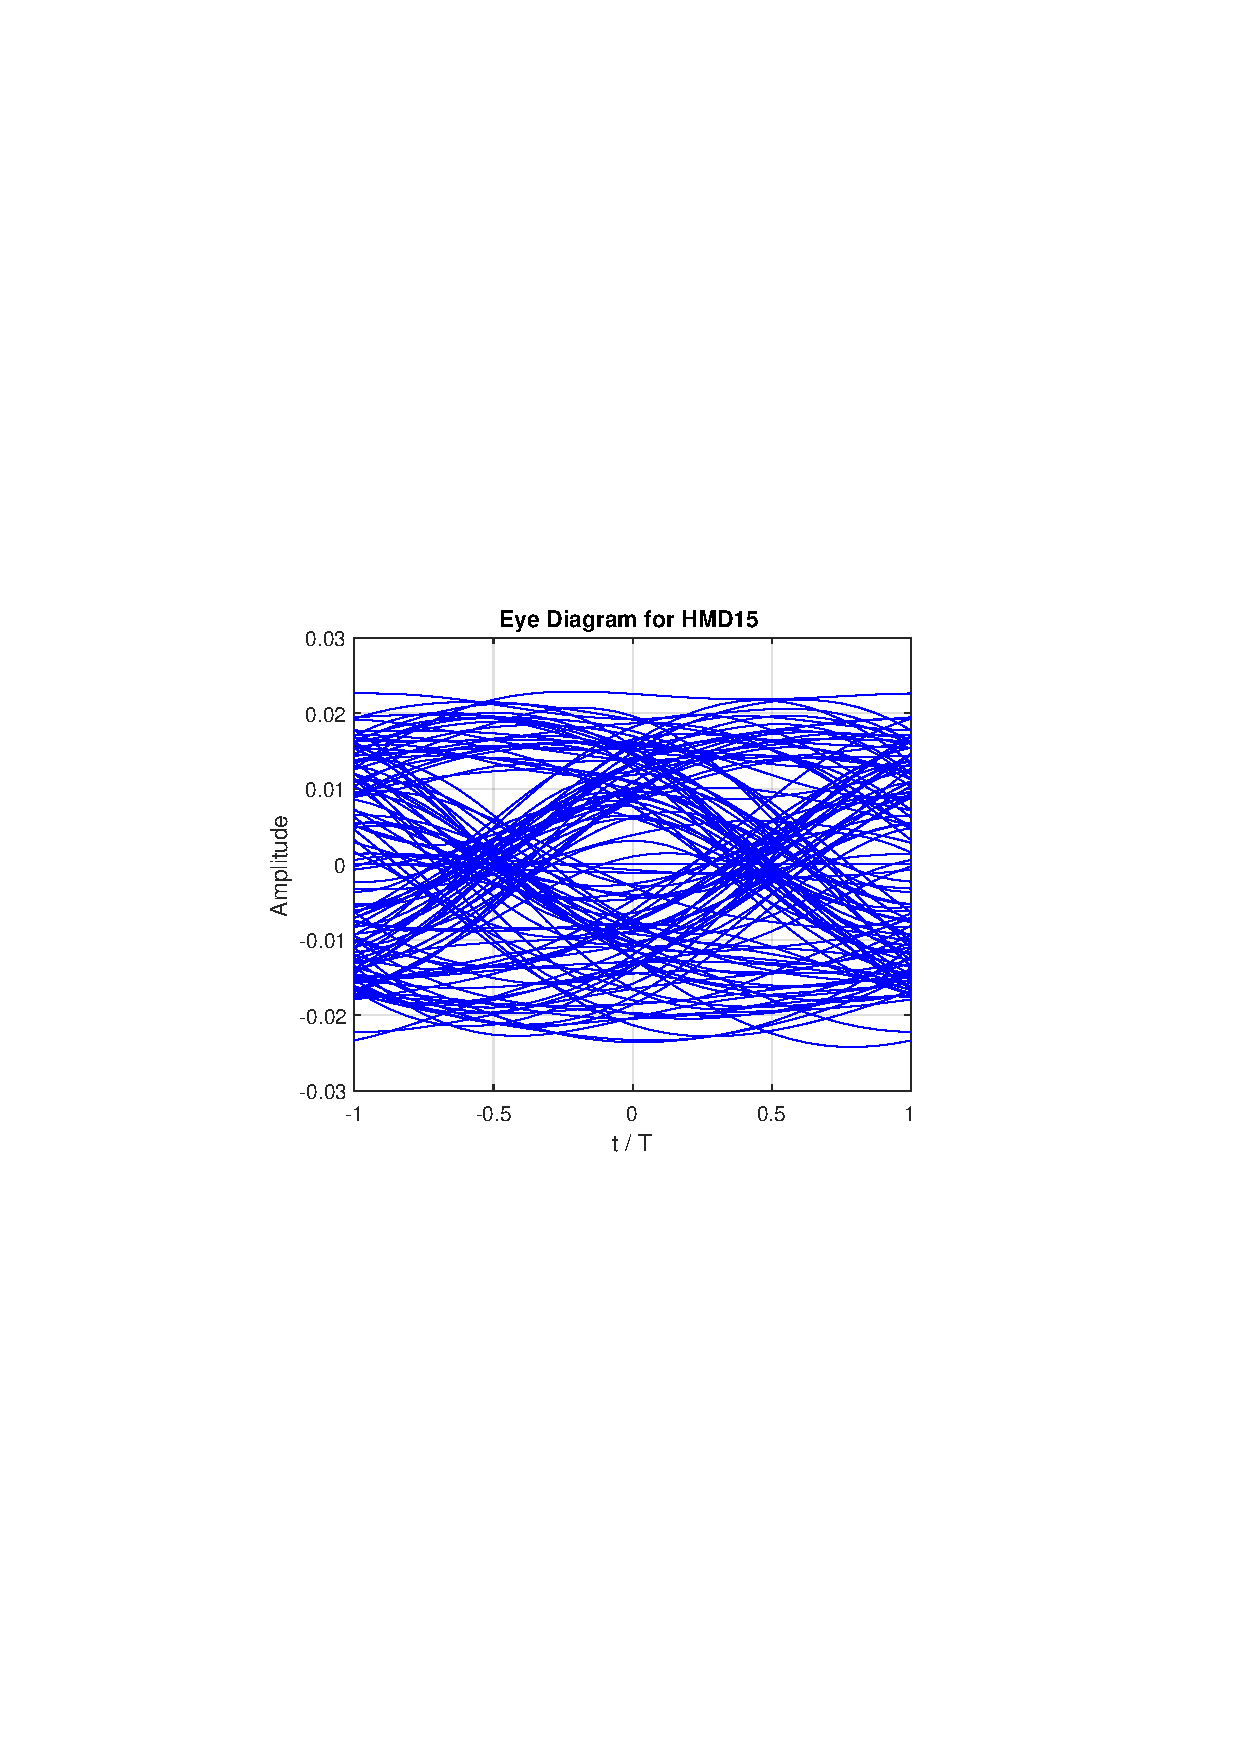
\includegraphics[clip, trim=5cm 10cm 5cm 10cm, width=\textwidth]{./sdf/m_qam_system/figures/HMD15_eye_diagram_60.pdf}
	\end{subfigure}
	\caption{Eye diagrams for the signals HMD14 (left) and HMD15 (right) for signalOutputPower\_dBm$=-60$. This corresponds to $\sqrt{\frac{E_b}{n_0}}=1$.}
	\label{fig:eye_diagram_60}
\end{figure}

\begin{figure}
	\centering
	\begin{subfigure}{.5\textwidth}
		\centering
		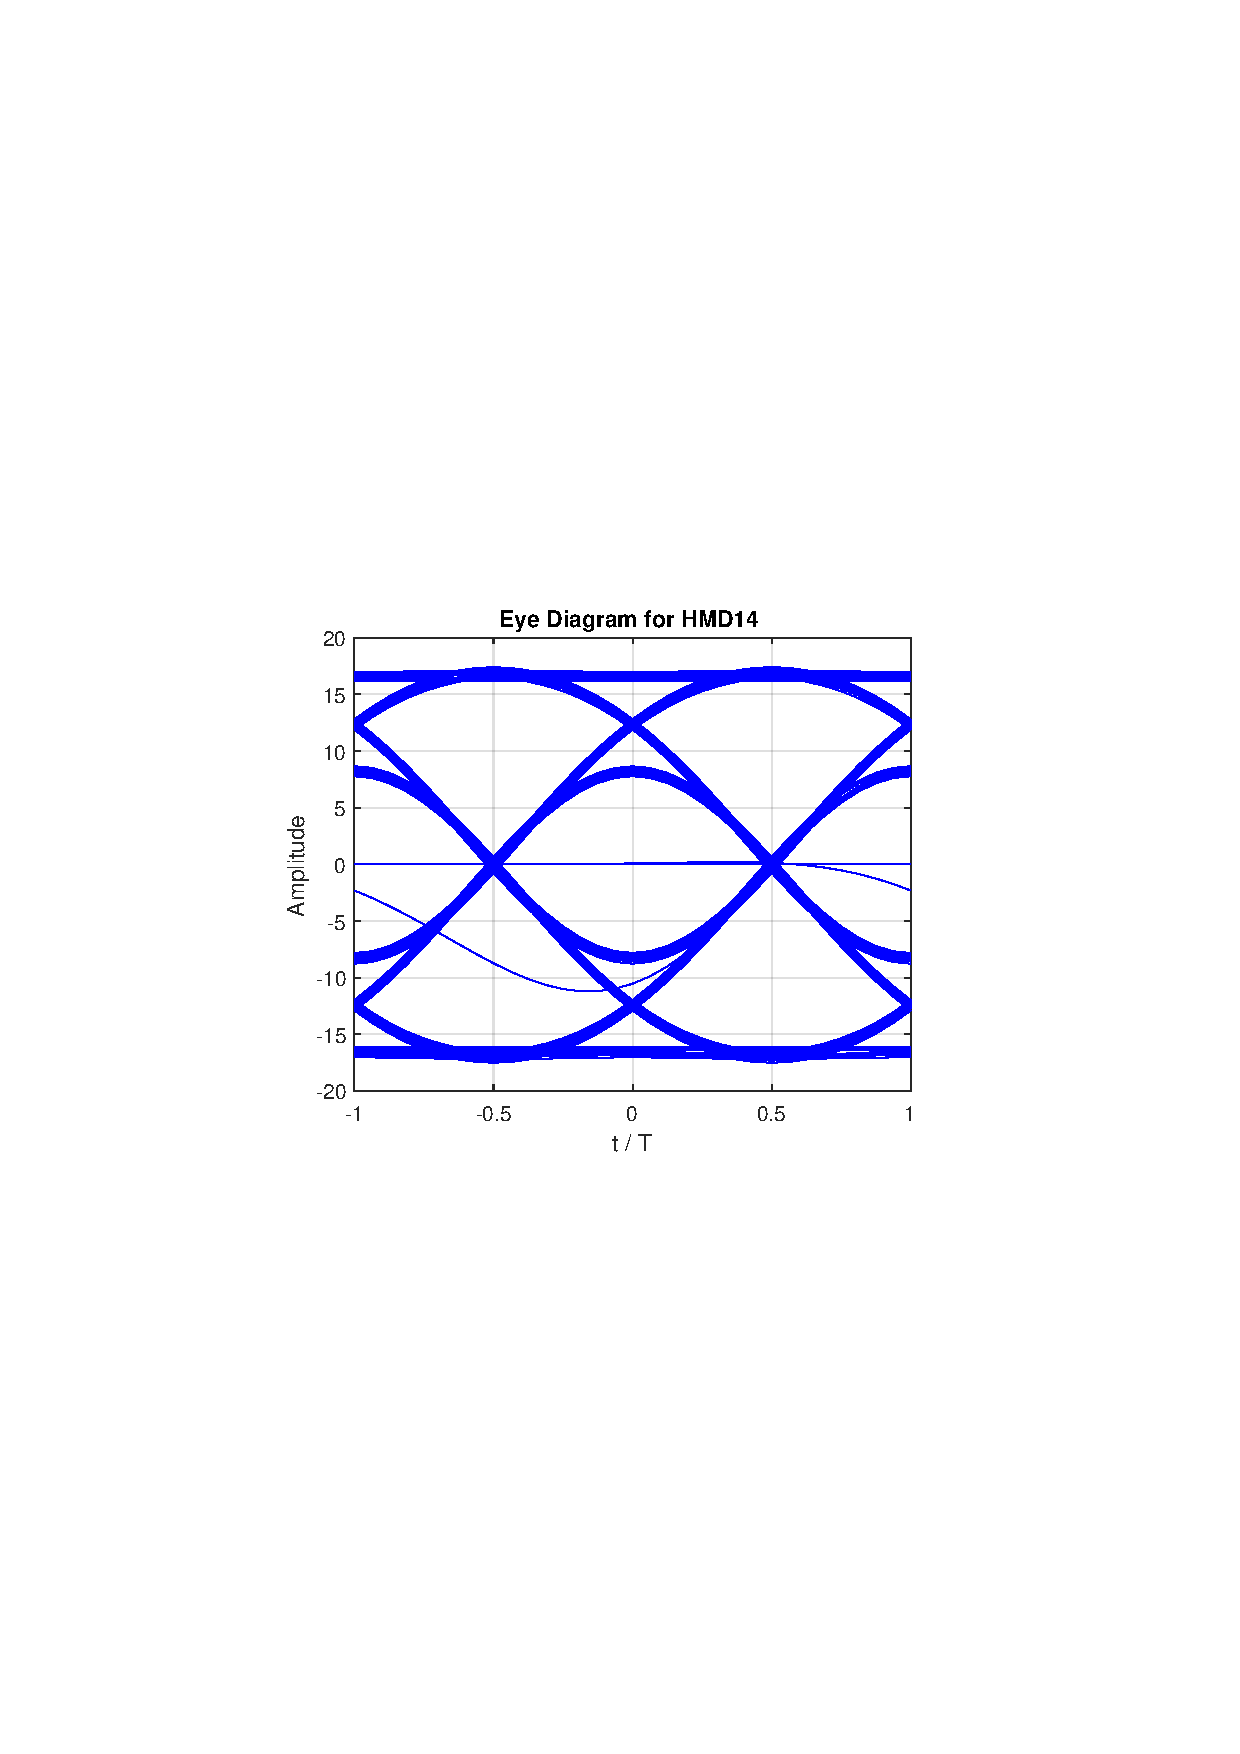
\includegraphics[clip, trim=5cm 10cm 5cm 10cm, width=\textwidth]{./sdf/m_qam_system/figures/HMD14_eye_diagram_0.pdf}
	\end{subfigure}%
	\begin{subfigure}{.5\textwidth}
		\centering
		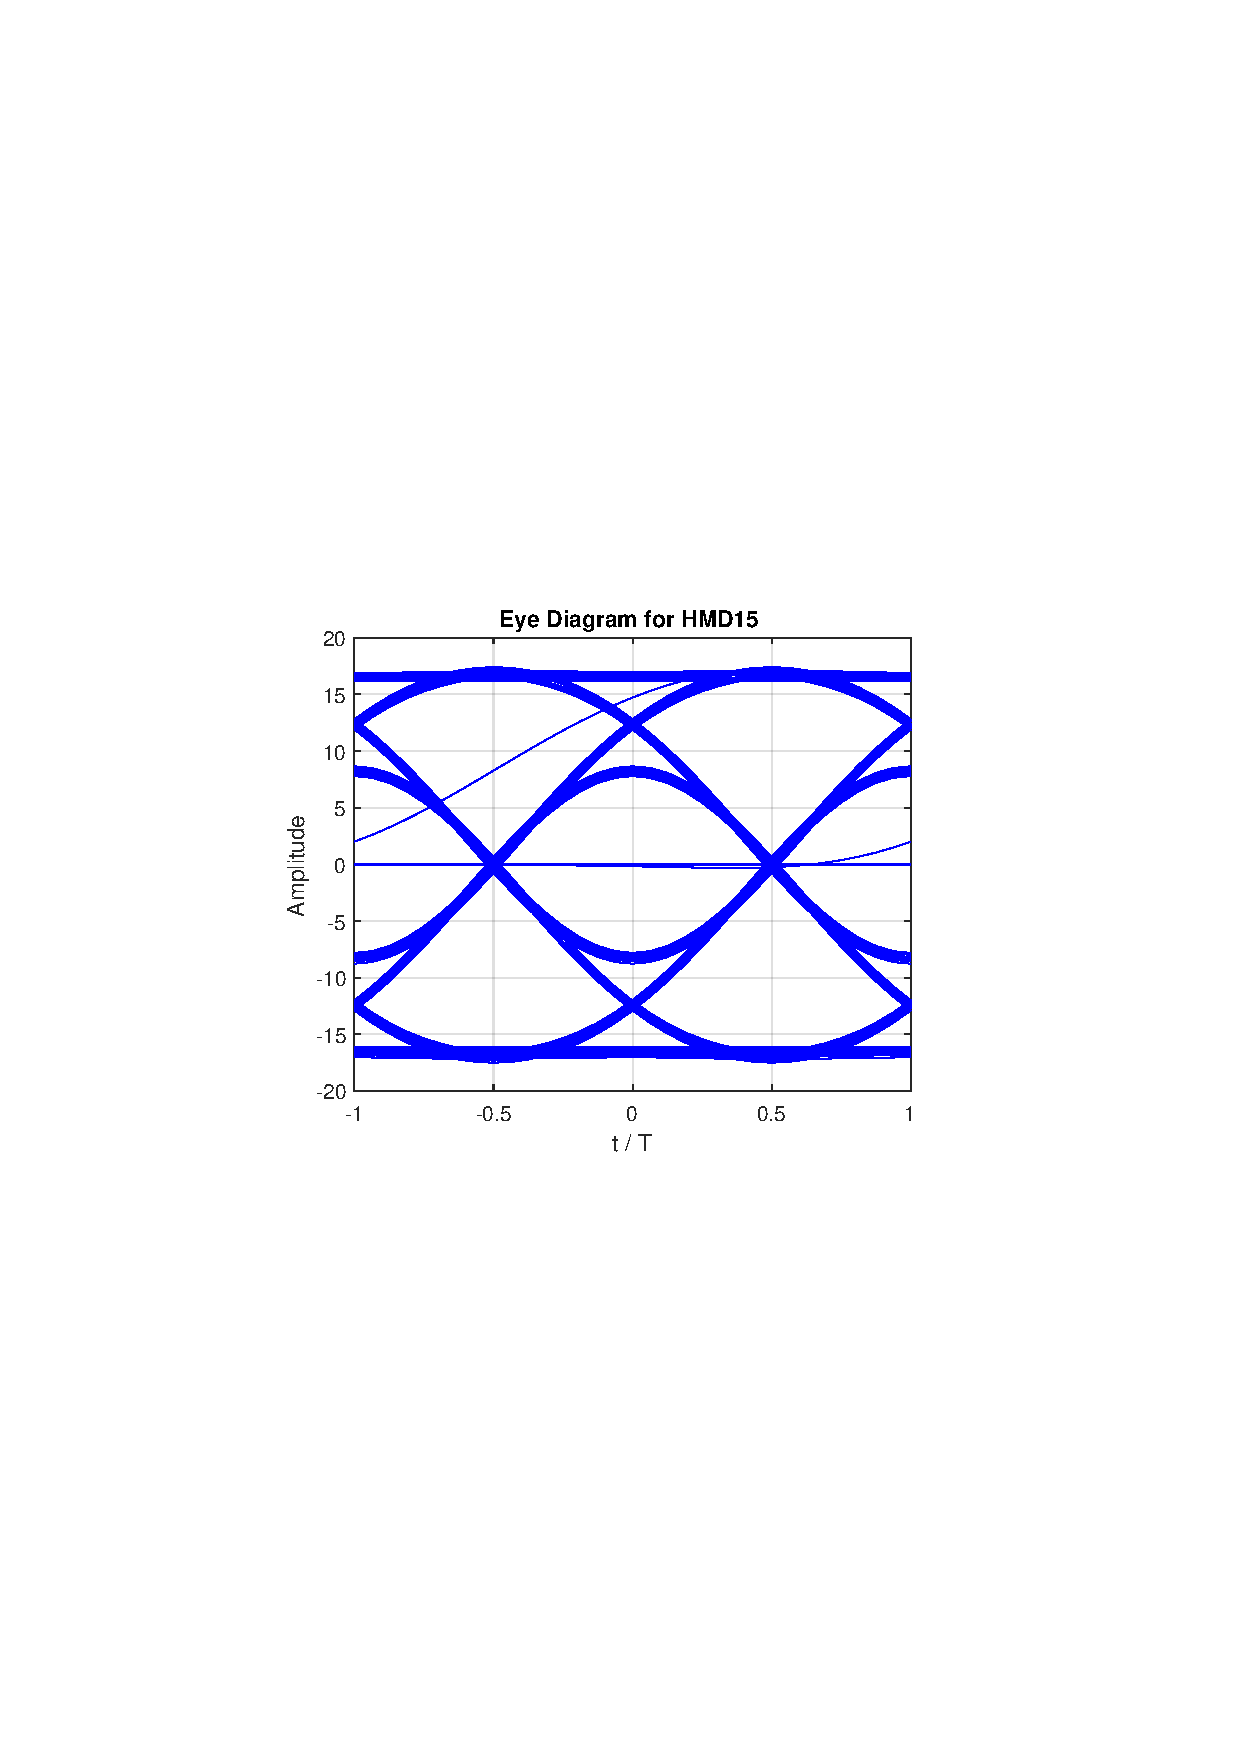
\includegraphics[clip, trim=5cm 10cm 5cm 10cm, width=\textwidth]{./sdf/m_qam_system/figures/HMD15_eye_diagram_0.pdf}
	\end{subfigure}
	\caption{Eye diagrams for the signals HMD14 (left) and HMD15 (right) for signalOutputPower\_dBm$=0$. This corresponds to $\sqrt{\frac{E_b}{n_0}}=10^{6}$.}
	\label{fig:eye_diagram_0}
\end{figure}

\begin{figure}[]
	\centering
	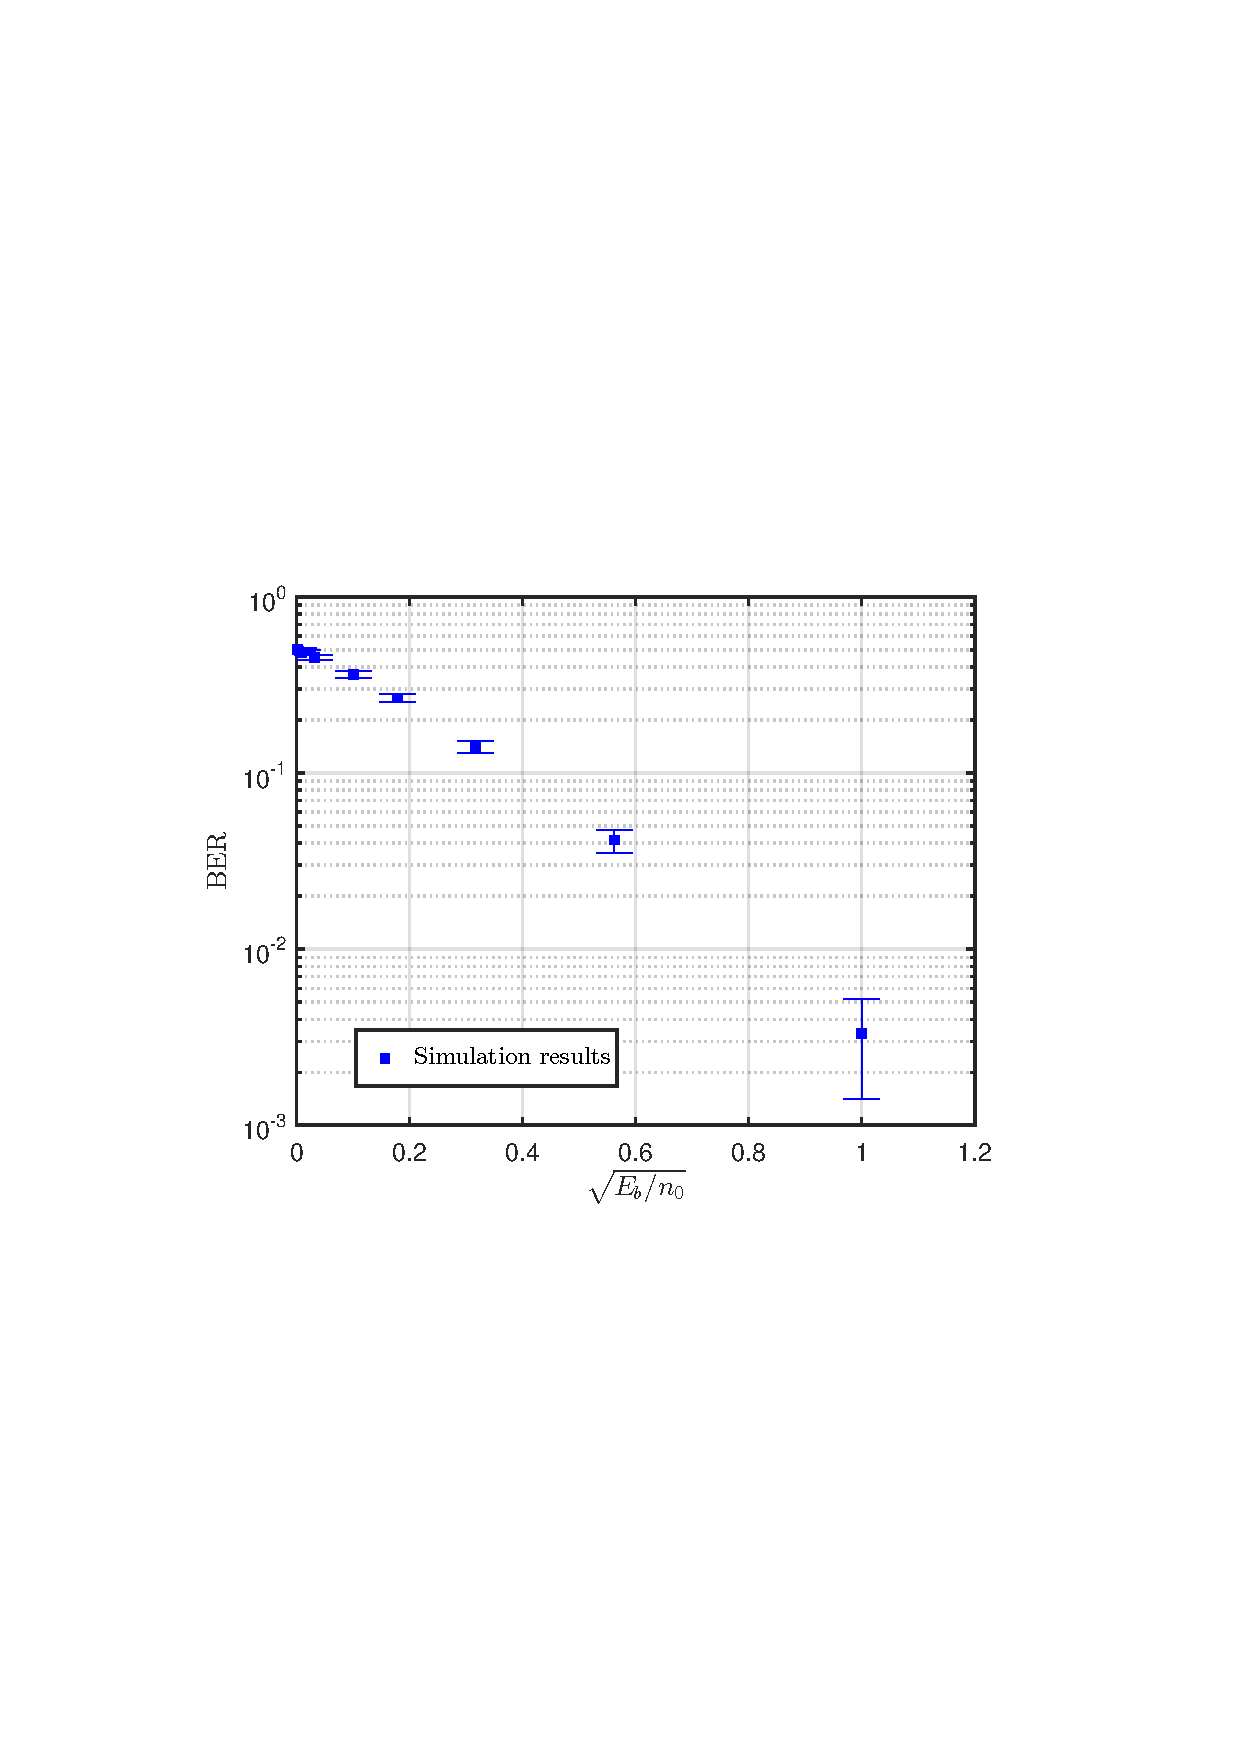
\includegraphics[clip, trim=0.5cm 9cm 0.5cm 9cm, width=\textwidth]{./sdf/m_qam_system/figures/BER_QPSK_sim_pseudorandom7_Eb_n0_onlySim.pdf}
	\caption{Simulation result for a random binary sequence with $4000$ bits, a noise amplitude of $10^{-6}$ and an amplification of $10^3$.}
	\label{fig:ber_pseudorandom_sim}
\end{figure}

\pagebreak
\clearpage
\newpage
\subsection{Comparative Analysis}

In this section we show the simulation results and compared them with the theoretical predictions. Figures \ref{fig:ber_pseudorandom} shows the variation of the BER with the power of the signal, using $4000$ bits and a pseudorandom binary sequence with pattern length $2^7$. To produce this plots we considered a noise amplitude of $10^{-6}$ and an amplification of $10^3$. 

\begin{figure}[h]
	\centering
	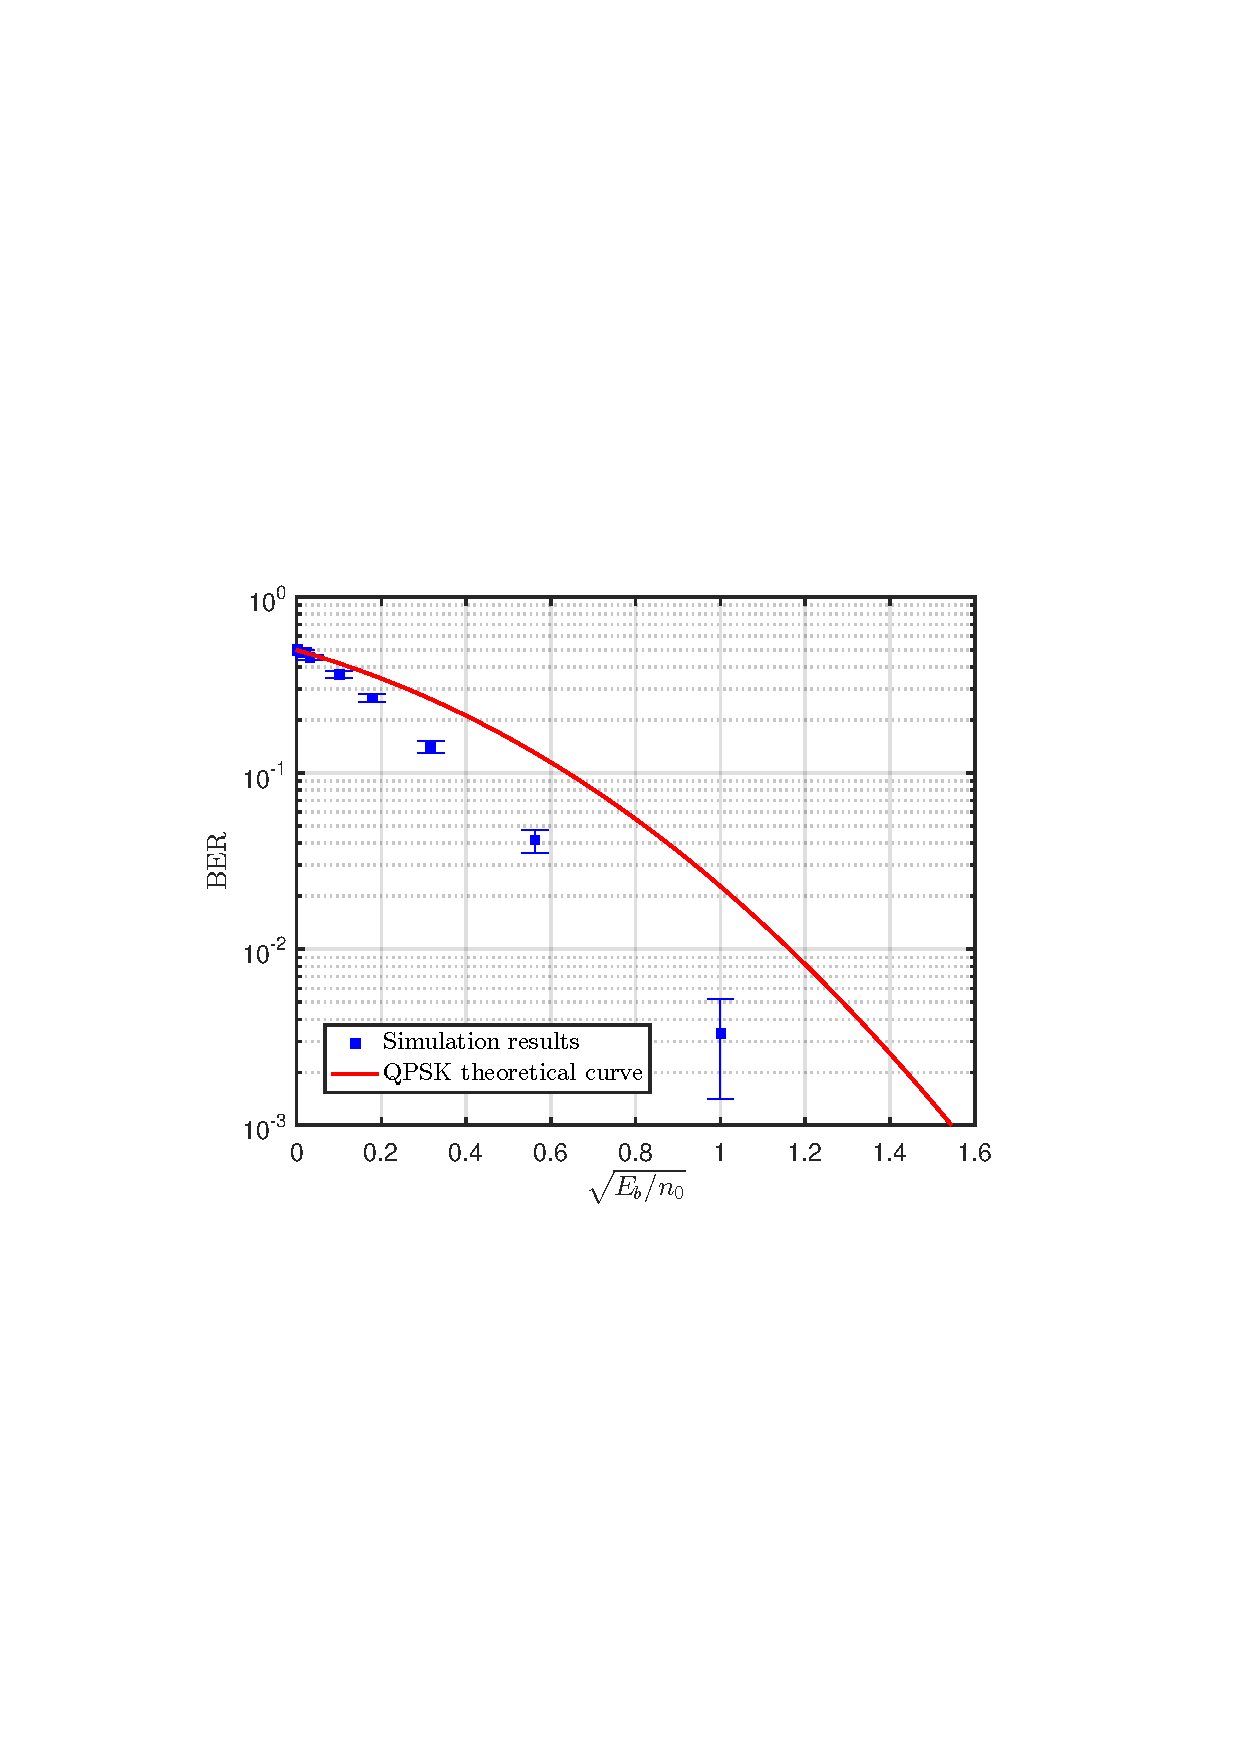
\includegraphics[clip, trim=0.5cm 9cm 0.5cm 9cm, width=\textwidth]{./sdf/m_qam_system/figures/BER_QPSK_sim_pseudorandom7_Eb_n0.pdf}
	\caption{Simulation result for a random binary sequence with $4000$ bits, a noise amplitude of $10^{-6}$ and an amplification of $10^3$.}
	\label{fig:ber_pseudorandom}
\end{figure}%

\subsection{Experimental setup}

In this section we show a schematic representation of the experimental setup. Here, BS and VOA stand for Beam Splitter and Variable Optical Attenuator, respectively.

\begin{figure}[h]
	\centering
	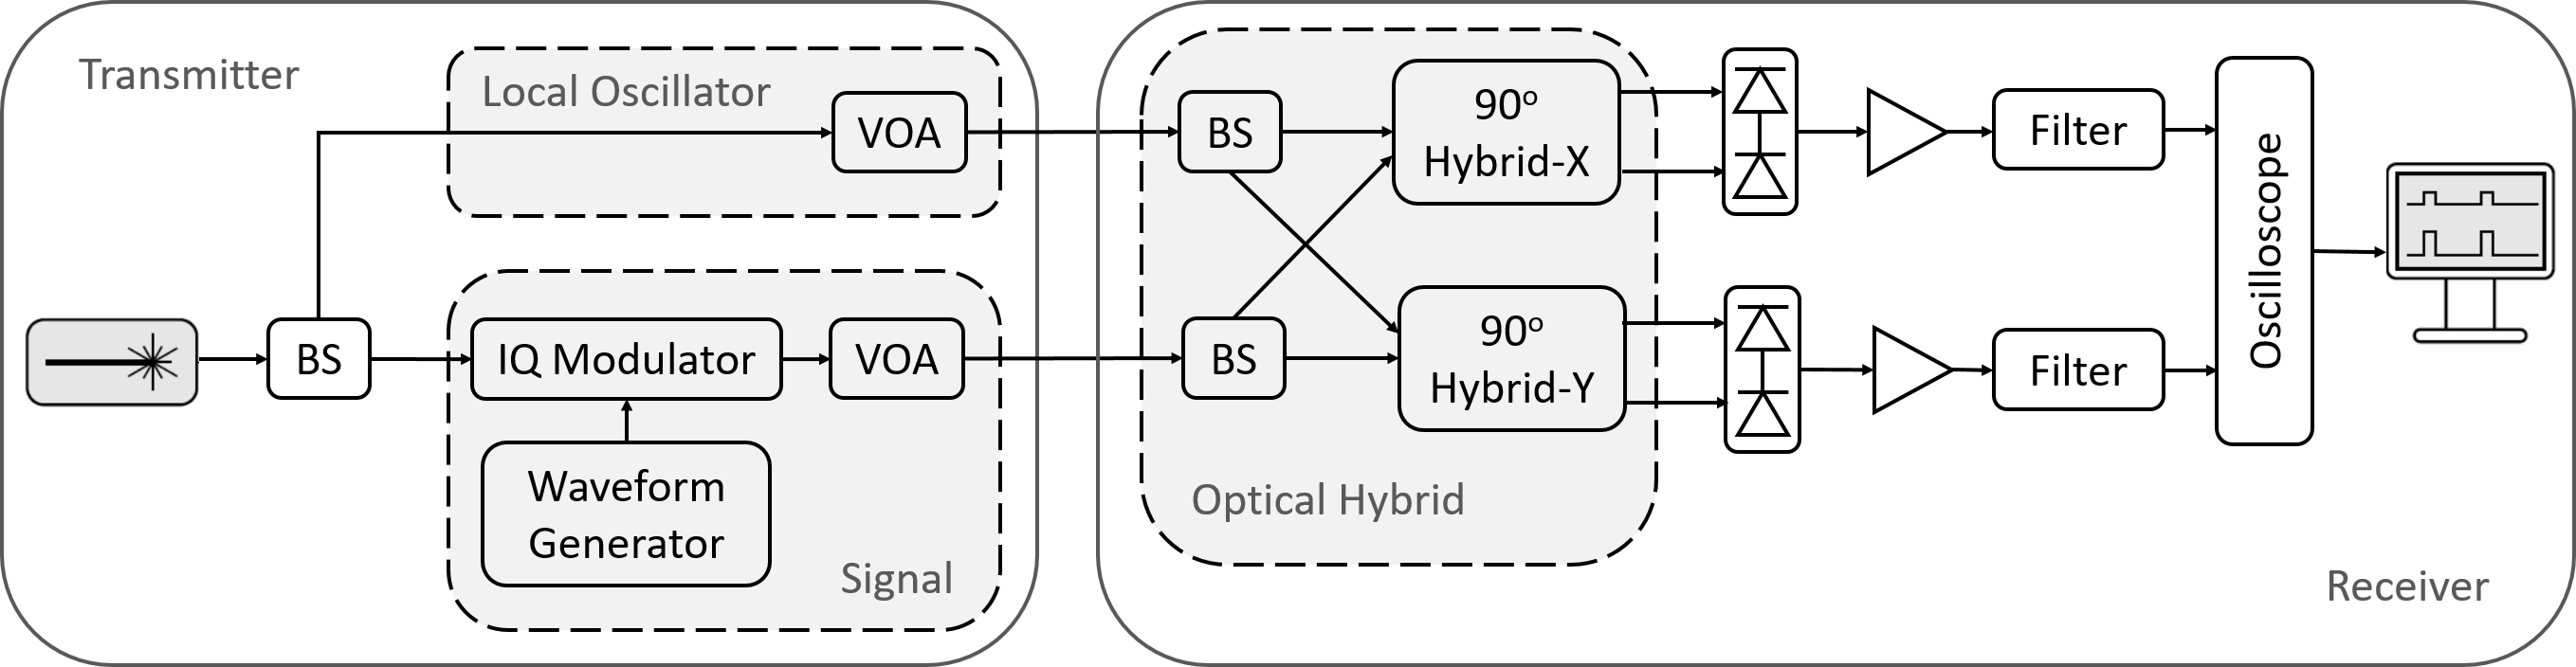
\includegraphics[width=\textwidth]{./sdf/m_qam_system/figures/experimental_setup.png}
	\caption{QPSK transmission system experimental setup}
	\label{fig:exp}
\end{figure}% \fi
\ifdefined\sdf          \clearpage
\section{Kramers-Kronig Transceiver  with Stokes PolDemux}

\begin{tcolorbox}	
\begin{tabular}{p{2.75cm} p{0.2cm} p{10.5cm}} 	
\textbf{Student Name}  &:& Romil Patel\\
\textbf{Starting Date} &:& August 16, 2017\\
\textbf{Goal}          &:& Develop a simplified structure (low cost) for a coherent transceiver, that can be used in coherent PON, inter-data center connections, or metropolitan networks (optical path lengths < 100 km). We are going to explore a Kramers-Kronig transceiver with Stokes based PolDemux.\\
\textbf{Directory} 	   &:&LinkPlanner\textbackslash doc\textbackslash tex\textbackslash sdf\textbackslash simplified\_coherent\_receiver 
\end{tabular}
\end{tcolorbox}

Coherent optical transmission schemes are spectrally efficient since they allow the encoding of information in both quadrature of sinusoid signal. However, the cost of coherent receiver becomes a major obstacle in the case of short-reach links applications like PON, inter-data-center communications and metropolitan network. In order to make the transceiver applicable in short-reach links, an architecture has been proposed which combines the advantages of coherent transmission and cost effectiveness of direct detection. The working principle of the proposed transceiver is based on the Kramers-Kronig (KK) relationship. The KK transceiver scheme allows digital compensation of propagation impairment because both amplitude and phase of the electrical field can be retrieved at the receiver. 
\subsection{Theoretical Analysis}
The Kramers-Kronig relations are bidirectional mathematical relations, connecting the real and imaginary parts of any complex function that is analytic in the upper half-plane. For instance, a signal $x(t)=x_r(t) + i x_i(t)$ satisfies the Kramers-Kronig relationship if,
\begin{equation*}
\begin{split}
x_{r}(t) &=-\frac{1}{\pi} p.v. \int_{-\infty}^{\infty} \frac{x_{i}(t')}{t-t'} dt' \\ \\
x_{i}(t) &=\frac{1}{\pi} p.v. \int_{-\infty}^{\infty} \frac{x_{r}(t')}{t-t'} dt' \\
\end{split}
\label{KK}
\end{equation*}
This relationship imposes that the real and the imaginary parts of the signal are related to each other though Hilbert transform. Therefore, if we have the real part of the signal then the imaginary part can be calculated by its Hilbert transform. \\For a signal that satisfies the Kramers-Kronig relationship, the real and imaginary part can be obtained only from the module. The following questions would give a comprehensive overview of Kramers-Kroning relation and the detailed mathematical calculation which depicts how phase can be extracted from the amplitude information.

\subsubsection{1. What is Hilbert transform?}
If we consider a filter $H(\omega)$, described in Figure \ref{Hilbert_Transformer}, that has a unity magnitude response for all frequencies and the phase response is $-\pi/2$ for all positive frequencies and $\pi/2$ for negative frequencies. The transfer function of this filter is given by
\begin{equation}
\begin{split}
H(\omega)=-isgn(\omega)
\end{split}
\label{}
\end{equation}
\begin{figure}[h]
	\centering
	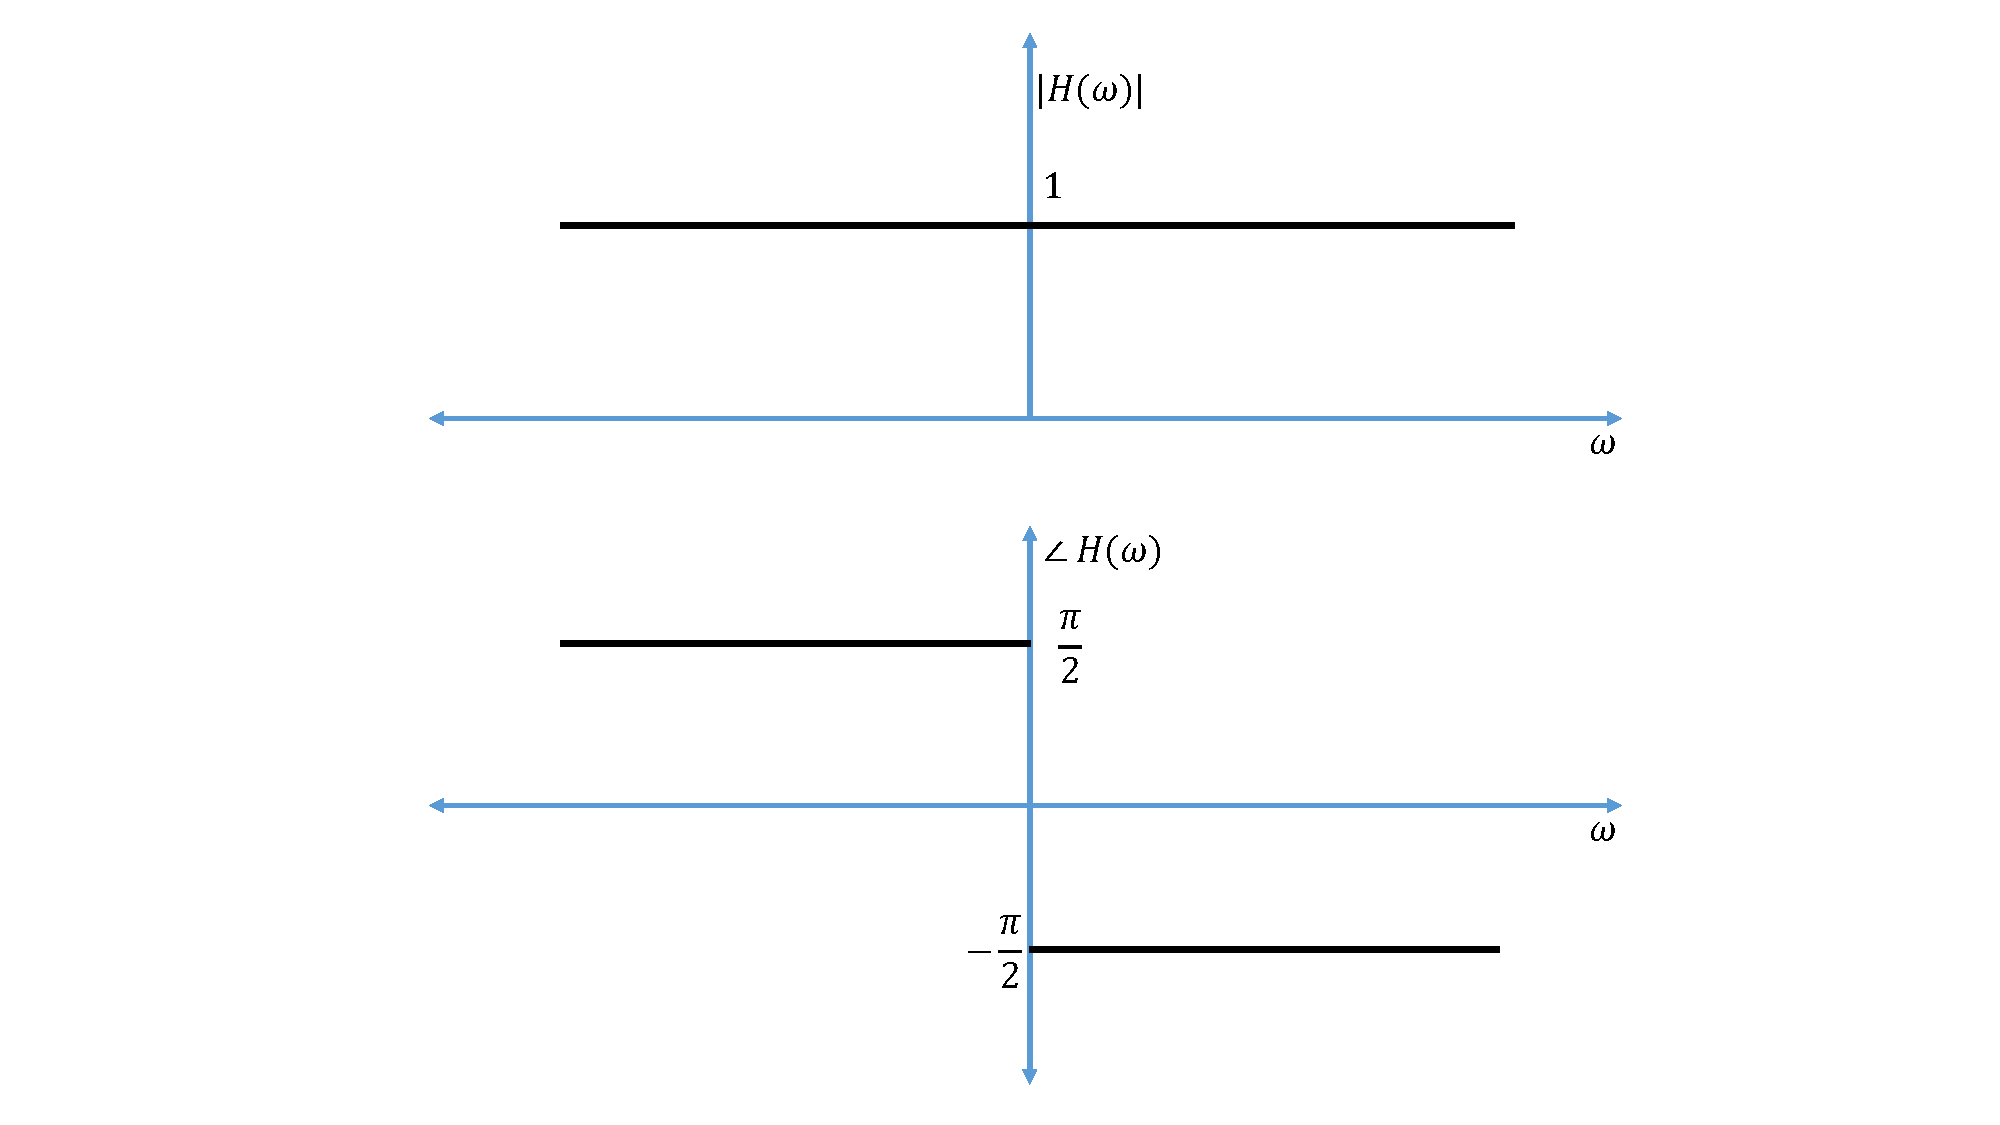
\includegraphics[width=1.0\textwidth, height=8cm]{./sdf/simplified_coherent_receiver/figures/HT.pdf}
	\caption{Magnitude and phase of Hilbert transform filter}\label{Hilbert_Transformer}
\end{figure}
\\
\\
\\
The inpulse response of this filter can be given as,

\begin{figure}[h]
	\centering
	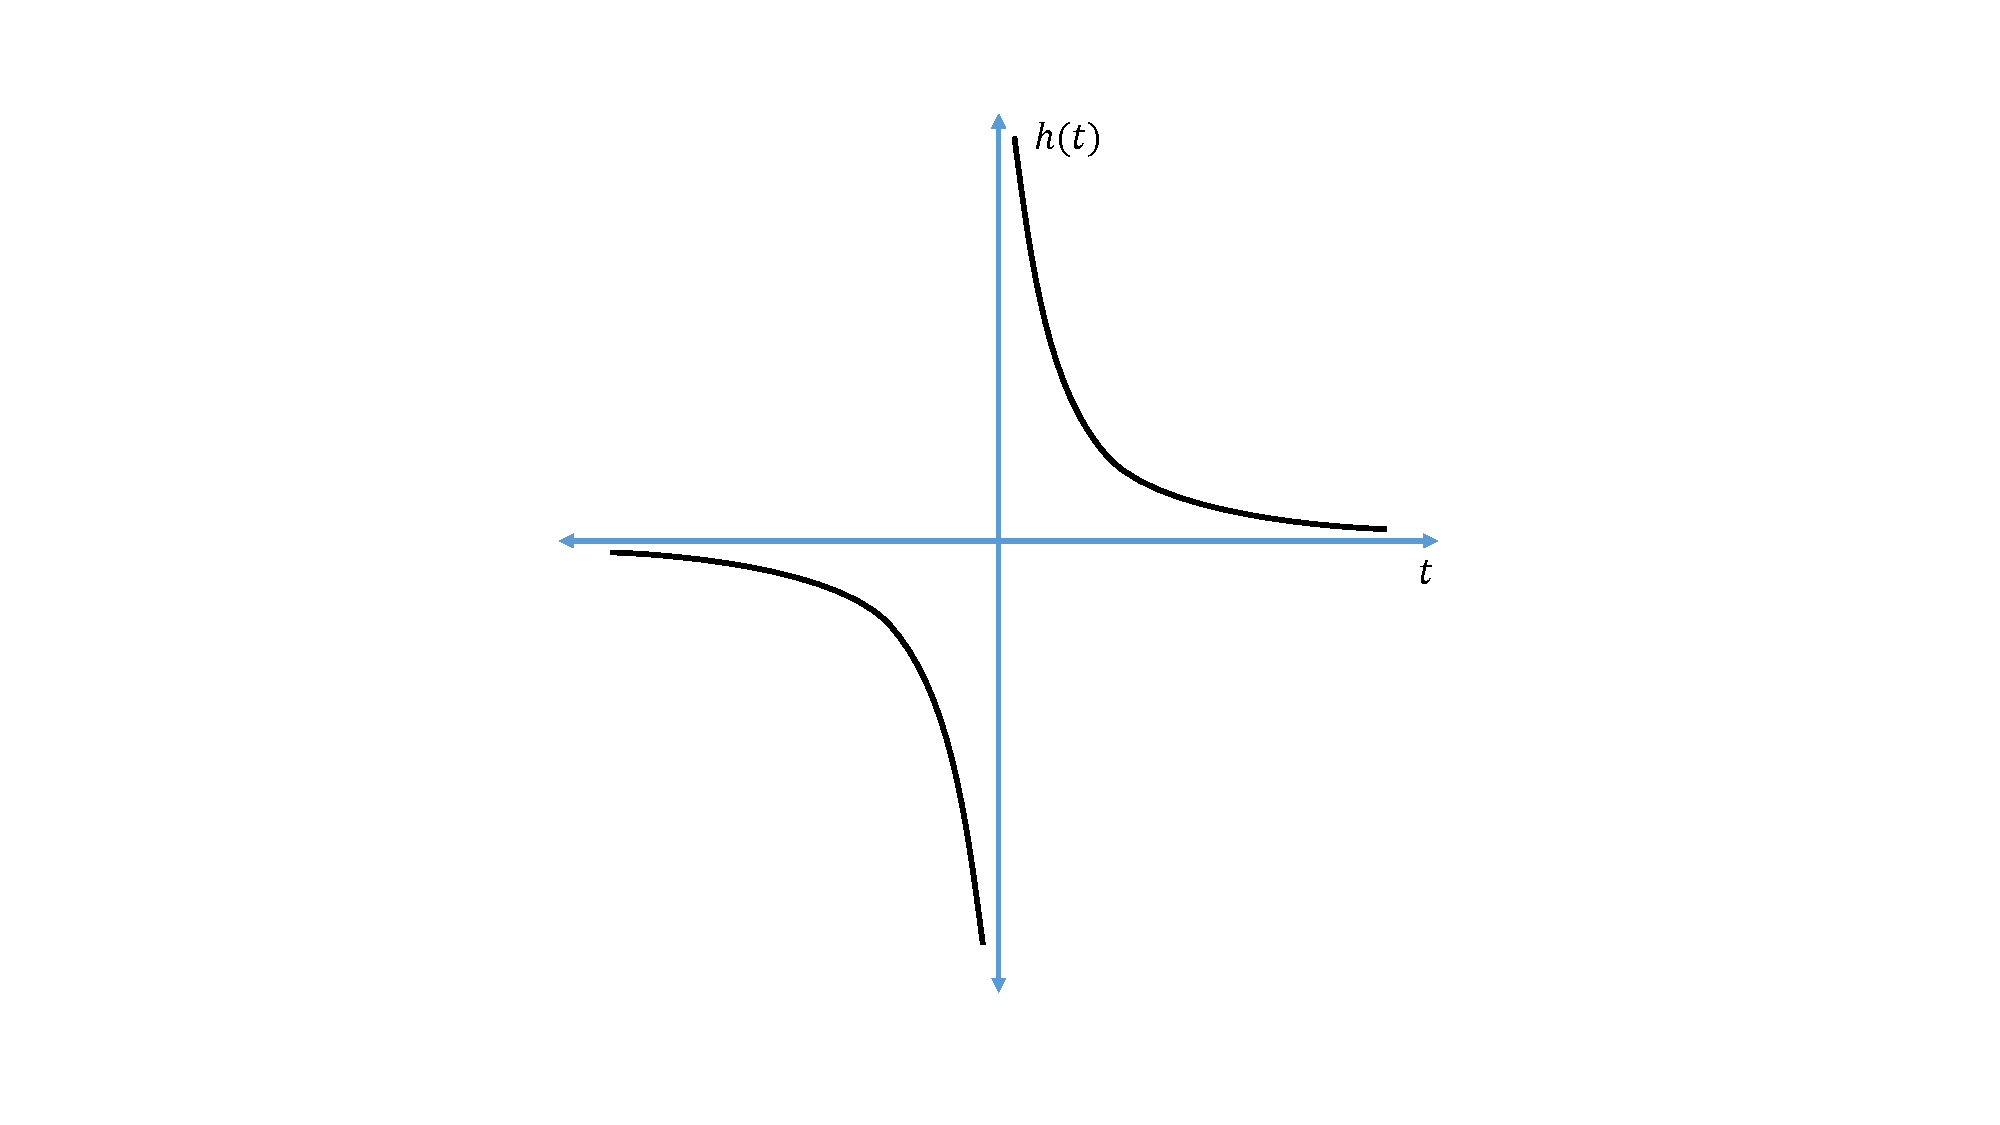
\includegraphics[width=1.0\textwidth, height=8cm]{./sdf/simplified_coherent_receiver/figures/Impulse_Response.pdf}
	\caption{Impulse response $h(t)$ of Hilbert transform filter}\label{Impulse_Response}
\end{figure}

\begin{equation}
\begin{split}
h(t)&=\mathcal{F}^{-1}[H(i\omega)]\\
&=-i\mathcal{F}^{-1}[sgn(\omega)]\\
&=-i\bigg(\frac{i}{\pi t}\bigg)\\
&=\frac{1}{\pi t}
\end{split}
\label{}
\end{equation}
When this filter driven by an arbitrary signal $s(t)$, the filter produces the output as,
\begin{equation}
\begin{split}
\hat{s}(t)&=s(t) * h(t)\\
&=\int_{-\infty}^{\infty} \dfrac{s(u)}{\pi(t-u)}du\\
\end{split}
\label{}
\end{equation}
The function $\hat{s}(t)$ is called the Hilbert transform if $s(t)$. Note that
\begin{equation}
\begin{split}
\mathcal{F}[\hat{s}(t)]=H(\omega)S(\omega)=-isgn(\omega)S(\omega)
\end{split}
\label{}
\end{equation}
In conclusion, if we convolve any time domain signal with $\frac{1}{\pi t}$ then it will give us Hilbert transformed signal in time domain. Similarly, from the convolution property of the Fourier transform, if we multiply $-isgn(\omega)$ with any frequency domain signal $S(\omega)$ then it'll give us Hilbert transformed signal in frequency domain.

\subsubsection{2. What is analytical signal?}
An analytic signal is a complex-valued signal that has no negative frequency components, and its real and imaginary parts are related to each other by the Hilbert transform.
\begin{equation}
s_a(t)=s(t)+i\hat{s}(t)
\label{Analytical signal}
\end{equation}
where, $s_a(t)$ is an analytical signal and $\hat{s}(t)$ is the Hilbert transform of the signal ${s}(t)$. Such analytical signal can be used to generate Single Sideband Signal (SSB) signal.

\subsubsection{3. What is a SSB signal and how it can be generated?}
By definition, the SSB is the signal which contains either upper sideband or lower sideband and hence it reduces the spectral occupancy by half. \\
This section will represent the brief idea of generating SSB signal using Hilbert transform method. To understand this, we may express signal $s(t)$ as a summation of the two complex-valued functions.
\begin{equation}
\begin{split}
s(t)&=\dfrac{1}{2}[s(t)+i\hat{s}(t)]+\dfrac{1}{2}[s(t)-i\hat{s}(t)]\\
\end{split}
\label{}
\end{equation}
From Equation \ref{Analytical signal},
\begin{equation}
\begin{split}
	s(t)&=s_a(t)+i{s_a^*}(t)
\end{split}
\label{}
\end{equation}
%where, the term $\dfrac{1}{2}[s(t)+i\hat{s}(t)]$ is the analytical representation of the signal $s(t)$ (from Equation \ref{Analytical signal}). Another term represents the complex conjugate $\dfrac{1}{2}[s(t)-i\hat{s}(t)]$ of this analytical signal.
Such representation of ${s_a}(t)$ and ${s_a^*}(t)$ divide the signal into non-negative frequency component and non-positive frequency component respectively. Considering only non-negative frequency ${s_a}(t)$ part, we can write it as
\begin{equation}
\dfrac{1}{2}{S_a}(f) = \begin{cases}
S(f) &\text{for $f>0$}\\
0    &\text{for $f<0$}\\
\end{cases}
\end{equation}
where ${S_a}(f)$ and ${S}(f)$ are the Fourier transform of ${t_a}(t)$ and ${s}(t)$ respectively. The frequency translated version of ${S_a}(f-f_0)$ contains only one side (positive) of ${S}(f)$ and hence it is called single sideband signal ${s_{ssb}}(t)$,
\begin{equation}
{F}^{-1}\{S_a(f-f_0)\}={s_a}(t) e^{i2\pi f_0 t}={s_{ssb}}(t)+i{\hat{s}_{ssb}(t)}
\end{equation}
Therefore, from the Euler's formula,
\begin{equation}
\begin{split}
{s}_{ssb}(t)&=Re\{s_a(t)  e^{i2\pi f_0 t}\}\\
&=Re\{[s(t)+i\hat{s}(t)] [cos(2\pi f_0t)+isin(2\pi f_0t)]\}\\
&=s(t)cos(2\pi f_0t)-\hat{s}(t)sin(2\pi f_0t)
\end{split}
\label{USB_SSB}
\end{equation}
This Equation \ref{USB_SSB} displays the mathematical modeling of the upper sideband SSB signal. Similarly, we can generate lower sideband SSB signal by,
\begin{equation}
{s}_{ssb}(t)=s(t)cos(2\pi f_0t)+\hat{s}(t)sin(2\pi f_0t)
\label{LSB_SSB}
\end{equation}

\subsubsection{4. What is minimum phase signal?}
A necessary and sufficient condition for a complex signal $A(t)$ to be minimum phase is that the curve described in a complex plane by $A(t)$ when $t\rightarrow -\infty$ to $t\rightarrow \infty$ \textbf{does not encircle the origin}. A minimum-phase signal has an useful property that the natural logarithm of the magnitude of the frequency response is related to the phase angle of the frequency response by the Hilbert transform.\\
For instance, if we consider a complex data-carrying signal whose spectrum is contained between $-B/2$ and $B/2$, and consider a SSB signal of the form,
\begin{equation}
x(t)=A + A_{s}(t)exp(-i\pi Bt)
\label{}
\end{equation}
where A is a constant. Here, $x(t)$ is minimum phase if and only if the winding number of its trajectory into complex plane is zero. The condition $|A|>|A_{s}(t)|$ is sufficient for guaranteeing minimum phase property [3]. 

\subsubsection{5. How we can use these signals and profit from them?}
This section represents the justification that why we need to use these signals into our proposed transceiver system.\\ \\
\textbf{Analytical Signal:}\\
If we denote an analytic signal $A_s(t)$ as, 
\begin{equation}
A_s(t)=A_{s,r}(t)+iA_{s,i}(t)
\label{Eq:5.31}
\end{equation}
then in the equation \ref{Eq:5.31}, the real and imaginary parts $A_{s,r}(t)$ and $A_{s,i}(t)$ are related through the Kramers-Kronig relation with each other. An intuitive way to analyze the relation is based on expressing its Fourier transform $A_s(\omega)$ as follows,
\begin{equation}
A_s(\omega)=\dfrac{1}{2}[1+sgn(\omega)]A_s(\omega)
\label{Eq:A}
\end{equation}
The equation \ref{Eq:A} follows the SSB signal condition $A_s(\omega)=0$ for $\omega<0$. Further, simplification0n of the signal can be summarized as follows:
\begin{equation}
\begin{split}
A_s(\omega)&=\dfrac{1}{2}[1+sgn(\omega)]A_s(\omega)\\
&=\dfrac{1}{2}A_s(\omega)+\dfrac{1}{2}sgn(\omega)A_s(\omega)
\end{split}
\label{Eq:B}
\end{equation}
Taking inverse Fourier transform of the equation \ref{Eq:B},
\begin{equation}
\begin{split}
{A_s}(t)&=IFT\{A_s(\omega)\}\\
&=\dfrac{1}{2}{A_s}(t)+\underline{\dfrac{1}{2}[IFT\{sgn(\omega)\} \circledast {A_s}(t)]}
\end{split}
\label{Eq:C}
\end{equation}
The underlined term in Equation \ref{Eq:C} displays that multiplication in frequency domain converted into the convolution in the time domain. Further, IFT of the function $sgn(\omega)$ given as $(-i/\pi t)$. As a consequences, we can further simplify our equation as,
\begin{equation}
\begin{split}
{A_s}(t)&=\dfrac{1}{2}{A_s}(t)+\frac{1}{2}\bigg[\frac{i}{\pi t} \circledast {A_s}(t) \bigg]\\
\frac{{A_s}(t)}{2} &=\frac{1}{2}\bigg[\frac{i}{\pi t} \circledast {A_s}(t) \bigg]\\
{A_s}(t) &=i\bigg[\frac{1}{\pi t} \circledast {A_s}(t) \bigg]\\
{A_s}(t) &=\frac{i}{\pi} p.v. \int_{-\infty}^{\infty} \frac{A_s(t')}{t-t'} dt' 
\end{split}
\label{Eq:D}
\end{equation}
Using Equation \ref{Eq:5.31} into Equation \ref{Eq:D},
\begin{equation}
\begin{split}
A_{s,r}(t)+iA_{s,i}(t) &=\frac{i}{\pi} p.v. \int_{-\infty}^{\infty} \frac{A_s(t')}{t-t'} dt' 
\end{split}
\label{Eq:5.36}
\end{equation}
Therefore,
\begin{equation}
\begin{split}
A_{s,r}(t)+iA_{s,i}(t) &=\frac{i}{\pi} p.v. \int_{-\infty}^{\infty} \frac{A_{s,r}(t')+iA_{s,r}(t')}{t-t'} dt' \\
A_{s,r}(t)+iA_{s,i}(t)&=-\frac{1}{\pi} p.v. \int_{-\infty}^{\infty} \frac{A_{s,i}(t')}{t-t'} dt' + \frac{i}{\pi} p.v. \int_{-\infty}^{\infty} \frac{A_{s,r}(t')}{t-t'} dt'
\end{split}
\label{Eq:5.37}
\end{equation}
which leads to,
\begin{equation}
\begin{split}
A_{s,r}(t) &=-\frac{1}{\pi} p.v. \int_{-\infty}^{\infty} \frac{A_{s,i}(t')}{t-t'} dt' \\
A_{s,i}(t) &=\frac{1}{\pi} p.v. \int_{-\infty}^{\infty} \frac{A_{s,r}(t')}{t-t'} dt' \\
\end{split}
\label{Eq:5.38}
\end{equation}\\
\textbf{Minimum Phase signal:}\\
Given function $A(t)=A_{s}(t)+\bar{A}$ never encircles the origin for $t\in(-\infty,\infty)$. if we define,
\begin{equation}
G(t)=log\bigg[\dfrac{A(t)}{\bar{A}}\bigg]\\
\label{Eq:A1}
\end{equation} 
then $G(\omega)$, the spectrum of $G(t)$, is such that $G(\omega)=0$ for $\omega<0$. Under the hypothesis stated by Equation \ref{Eq:5.36}, we can write $G(t)$ as,
\begin{equation}
\begin{split}
G(t) &=\frac{i}{\pi} p.v. \int_{-\infty}^{\infty} \frac{G(t')}{t-t'} dt' 
\end{split}
\label{Eq:B1}
\end{equation}
From the equations \ref{Eq:A1} and \ref{Eq:B1},
\begin{equation}
\begin{split}
log|A(t)|-log|\bar{A}|+i[\phi(t)-\bar{\phi}] &=\frac{i}{\pi} p.v. \int_{-\infty}^{\infty} \frac{log|A(t)|-log|\bar{A}|}{t-t'} dt' + \frac{1}{\pi} p.v. \int_{-\infty}^{\infty} \frac{\phi(t)-\bar{\phi}}{t-t'} dt' 
\end{split}
\label{Eq:C1}
\end{equation}
Comparing Imaginary part of Equation \ref{Eq:C1},
\begin{equation}
\begin{split}
\phi(t)-\bar{\phi} &= + \frac{1}{\pi} p.v. \int_{-\infty}^{\infty} \frac{log|A(t)|-log|\bar{A}|}{t-t'} dt'\\
\end{split}
\label{Eq:D1}
\end{equation}
In equation \ref{Eq:D1}, $\frac{1}{\pi} p.v. \int_{-\infty}^{\infty} \frac{log|\bar{A}|}{t-t'} dt'=0$ which leads to,
\begin{equation}.
\begin{split}
\phi(t) &= \bar{\phi} + \frac{1}{\pi} p.v. \int_{-\infty}^{\infty} \frac{log|A(t)|}{t-t'} dt'\\
\phi(t) &= \bar{\phi} + \frac{1}{2\pi} p.v. \int_{-\infty}^{\infty} \frac{log|A(t)|^2}{t-t'} dt'\\
\end{split}
\label{Eq:E1}
\end{equation}
\newpage
\subsection{Simulation Analysis}
\subsubsection{Transmitter setup}
\begin{center}
\begin{figure}[h]
	\centering
	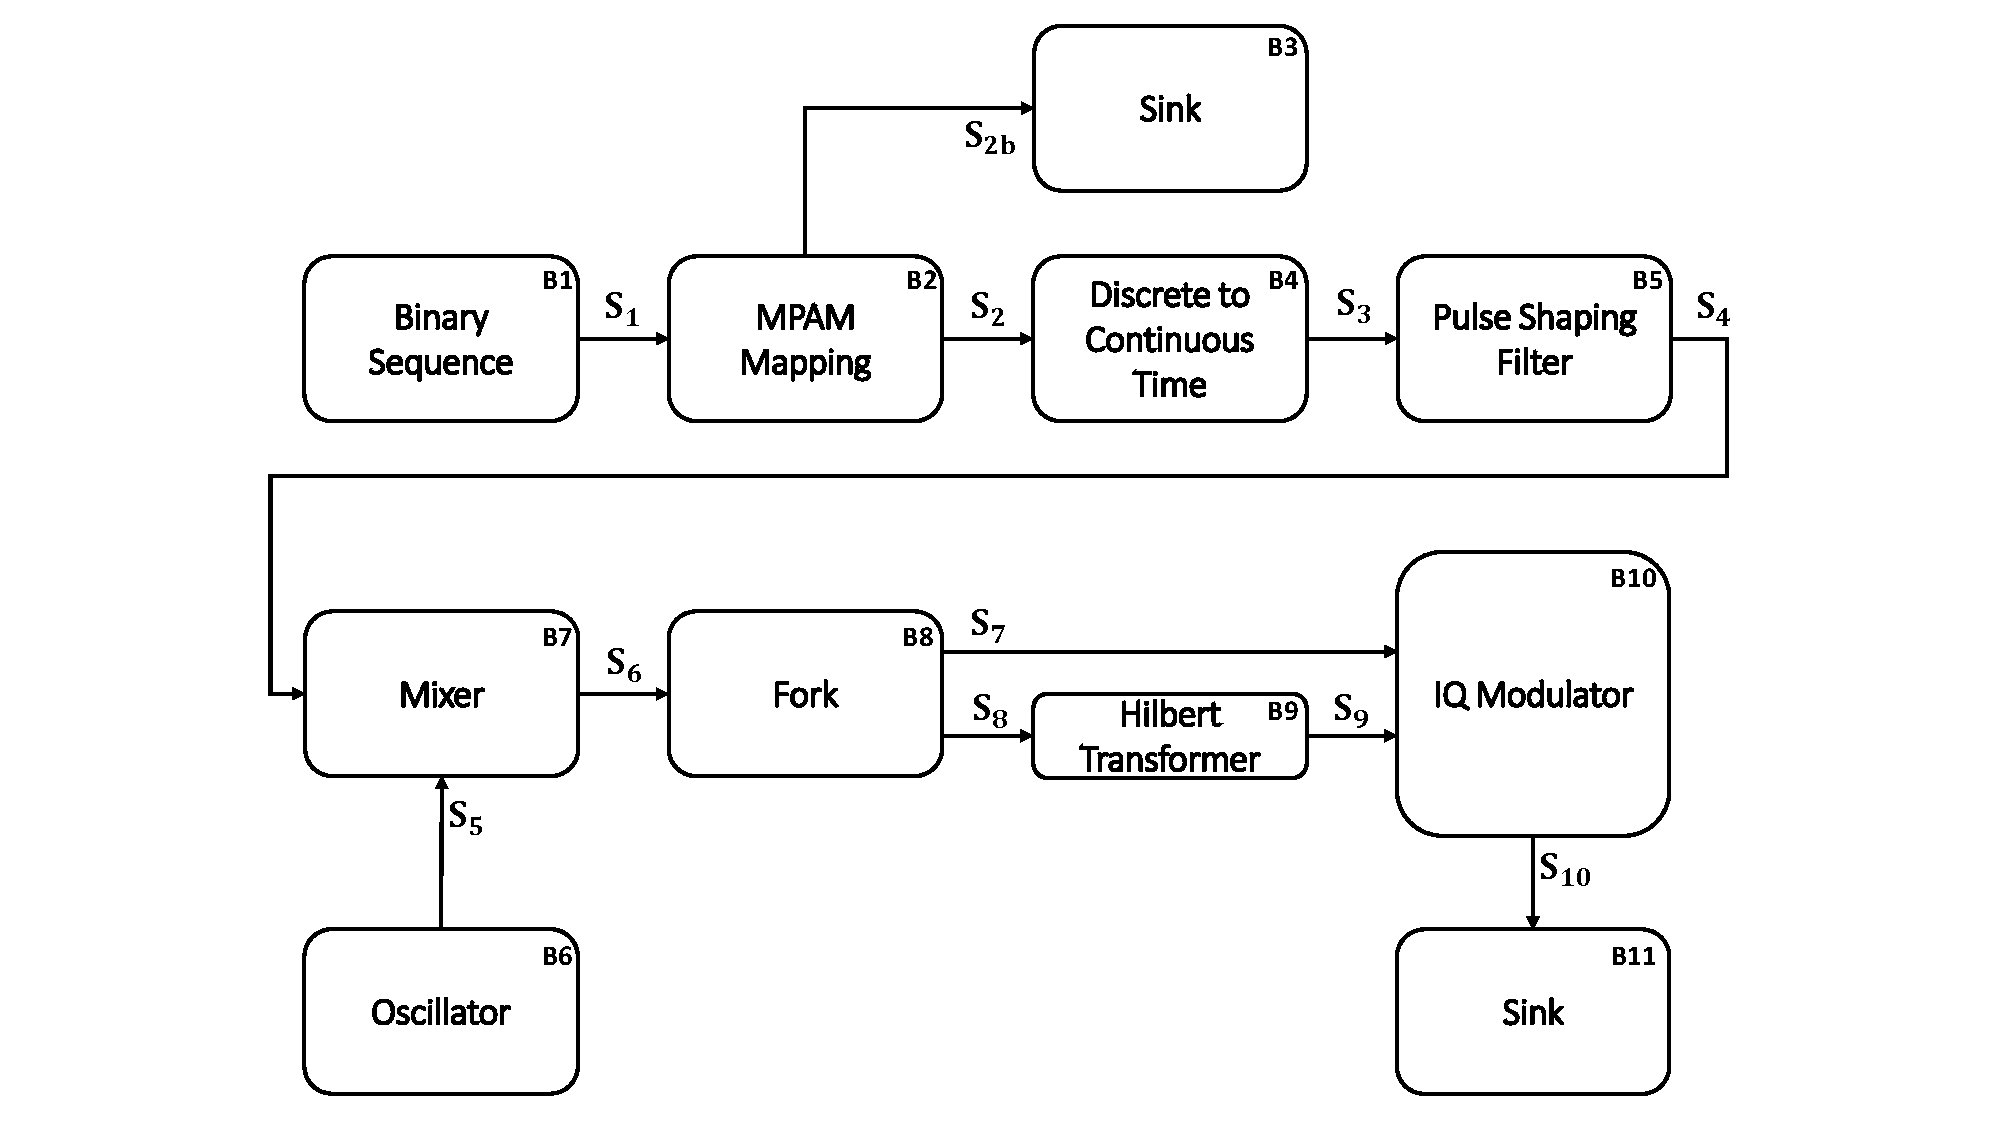
\includegraphics[width=1\textwidth, height=9cm]{./sdf/simplified_coherent_receiver/figures/Simulation_setup_Tx.pdf}
	\caption{Transmitter simulation setup}\label{Simulation_setup_Tx}
\end{figure}
\end{center}
\subsubsection{System input parameters:}
\begin{center}
	\begin{tabular}{ |p{5cm}||p{4.5cm}|p{4.5cm}|  }
		\hline
		%\multicolumn{3}{|c|}{\textbf{System Input Parameters }} \\
		%\hline
		\textbf{Parameter} &  \textbf{Default Value} & \textbf{Description}\\
		\hline
		sourceMode    & PseudoRandom &\\
		\hline
		patternLength & 5      & \\
		\hline
		bitPeriod     & 1/1.25e9 & \\
		\hline
		iqAmplitudes  &\{\{0,0\},\{1,0\},\{2,0\},\{3,0\}\} &\\
		\hline
		numberOfBits  &   1000 & \\
		\hline
		numberOfSamplesPerSymbol& 16  &\\
		\hline
		rollOffFactor & 0.3    & \\
		\hline
		impulseResponseTimeLength&16&\\
		\hline
		rfFrequency& 1.25e9 &\\
		\hline
		outputOpticalPower&1e-3&\\
		\hline
		rfAmplitude{ 1.0 }& 1.0 &\\
		\hline
		rfInitialPhase & 0.0 &\\
		\hline
		outputOpticalWavelength & 1550e-9 &\\
		\hline
		opticalPower & 1e-3 &\\
		\hline
%		outputOpticalWavelength&1550e-9&\\
%		\hline
	\end{tabular}
\end{center}
\vspace{0cm}
\subsubsection{Transmitter setup description:}
\begin{center}
	\begin{tabular}{ |p{6cm}||p{5.5cm}|p{2.5cm}|   }
		\hline
		\multicolumn{3}{|c|}{\textbf{Header Files}} \\
		\hline
		\textbf{File name} & \textbf{Comments}&\textbf{Code Status}\\
		\hline
		binary\_source.h    				&  	Integrated	&\checkmark\\
		\hline
		m\_qam\_mapper.h 					&Integrated \hspace{5mm} NEW! &\checkmark\\
		\hline
		discrete\_to\_continuous\_time.h    &  Integrated		&\checkmark\\
		\hline
		pulse\_shaper.h 					& 	Integrated	&\checkmark\\
		\hline
		RF\_Oscillator.h					&Integrated \hspace{5mm} NEW! &\checkmark\\
		\hline
		mixer.h		 						&Integrated \hspace{5mm} NEW! &\checkmark\\
		\hline
		fork.h								&Integrated \hspace{5mm} NEW! &\checkmark\\
		\hline
		hilbert\_transform.h				&Integrated \hspace{5mm} NEW! &\checkmark\\
		\hline
		iq\_modulator.h						&  		&\checkmark\\
		\hline
		sink.h								&  Integrated	&\checkmark\\
		\hline
		netxpto.h							&  Integrated		&\checkmark\\
		\hline
	\end{tabular}
\end{center}
\vspace{0.4cm}
\begin{center}
	\begin{tabular}{ |p{6cm}||p{5.5cm}|p{2.5cm}|   }
		\hline
		\multicolumn{3}{|c|}{\textbf{Source Files}} \\
		\hline
		\textbf{File name} & \textbf{Comments}&\textbf{Code Status}\\
		\hline
		binary\_source.cpp    				& Integrated &\checkmark\\
		\hline
		m\_qam\_mapper.cpp 					& Integrated \hspace{5mm} NEW! &\checkmark\\
		\hline
		discrete\_to\_continuous\_time.cpp  & Integrated &\checkmark\\
		\hline
		pulse\_shaper.cpp 					& Integrated &\checkmark\\
		\hline
		RF\_Oscillator.cpp					& Integrated \hspace{5mm} NEW! &\checkmark\\
		\hline
		mixer.cpp		 					& Integrated \hspace{5mm} NEW! &\checkmark\\
		\hline
		fork.cpp							& Integrated \hspace{5mm} NEW! &\checkmark\\
		\hline
		hilbert\_transform.cpp				& Integrated \hspace{5mm} NEW! &\checkmark\\
		\hline
		iq\_modulator.cpp					&  &\checkmark\\
		\hline
		sink.cpp							& Integrated &\checkmark\\
		\hline
		netxpto.cpp							& Integrated  &\checkmark\\
		\hline
		kramers\_kronig\_transceiver\_sdf.cpp  & Integrated &\checkmark\\
		\hline
	\end{tabular}
\end{center}
\newpage
\subsubsection{Simulation results:}

\begin{figure}[h]
	\centering
	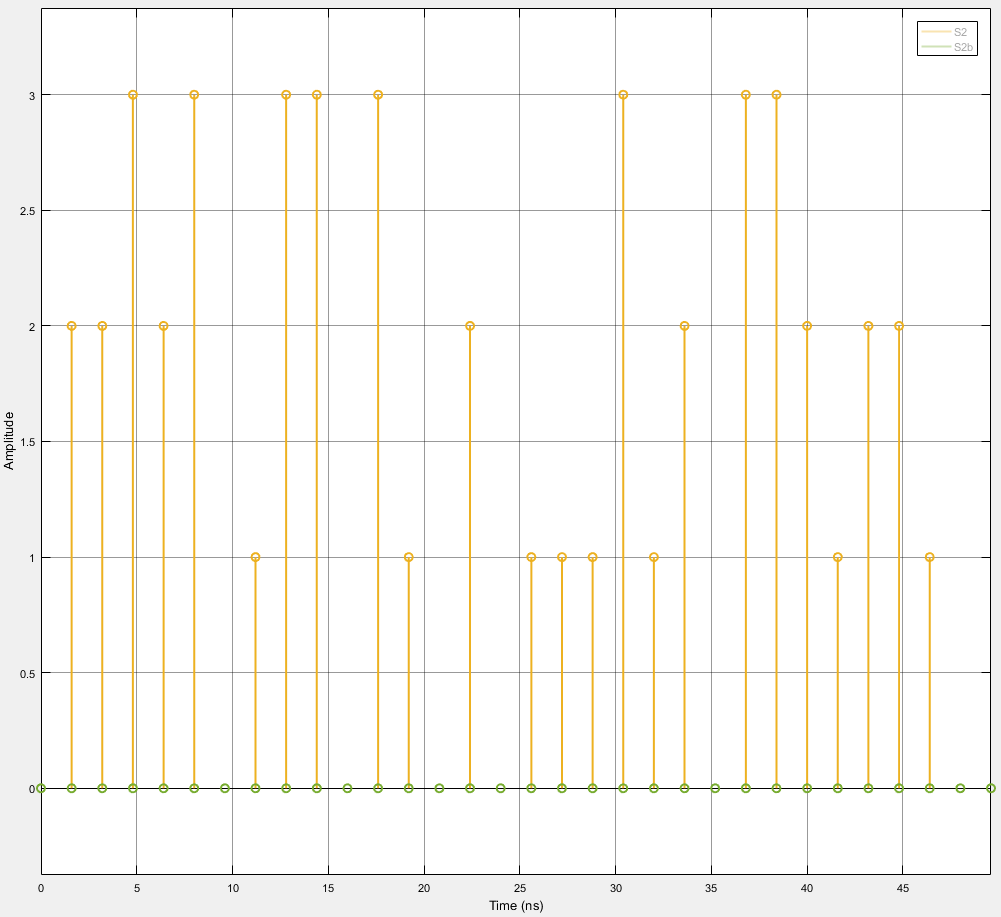
\includegraphics[width=0.9\textwidth, height=9cm]{./sdf/simplified_coherent_receiver/figures/S2S2b.png}
	\caption{S2 and S2b}\label{}
\end{figure}

\begin{figure}[h]
	\centering
	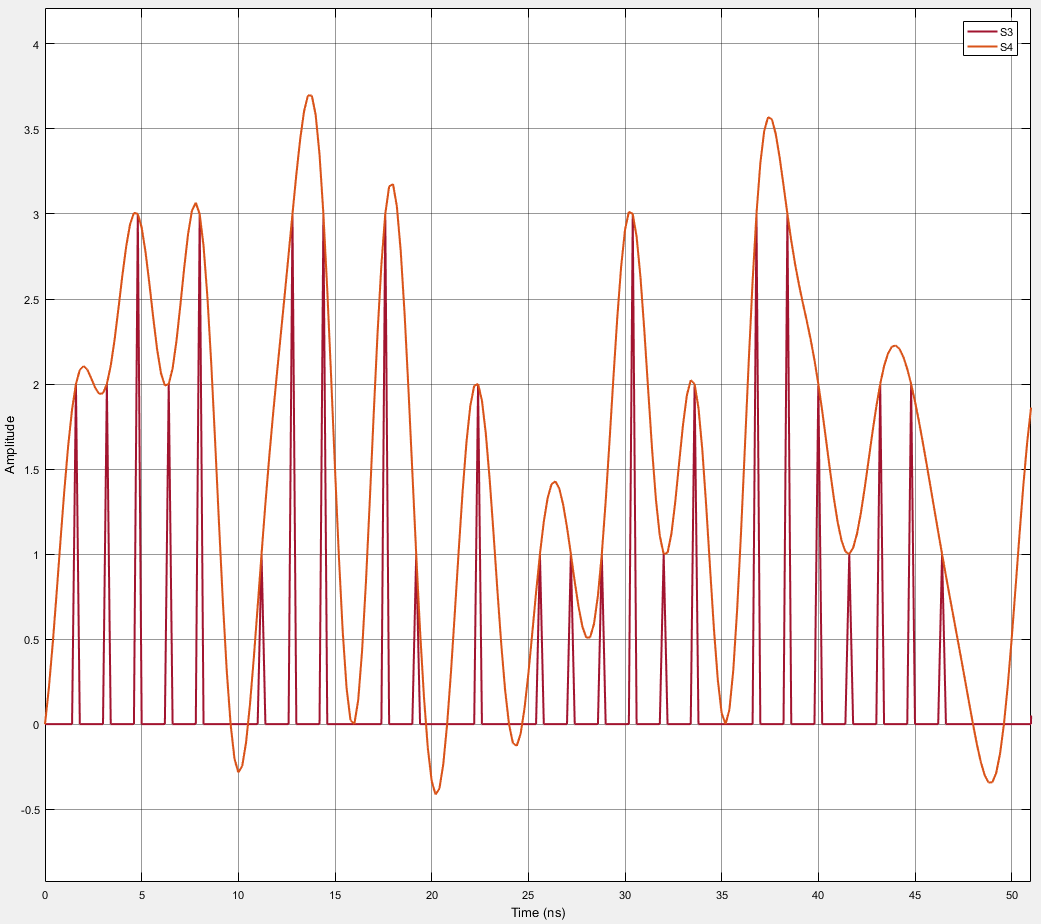
\includegraphics[width=0.9\textwidth, height=9cm]{./sdf/simplified_coherent_receiver/figures/S3S4.png}
	\caption{S3 and S4}\label{}
\end{figure}

\begin{figure}[h]
	\centering
	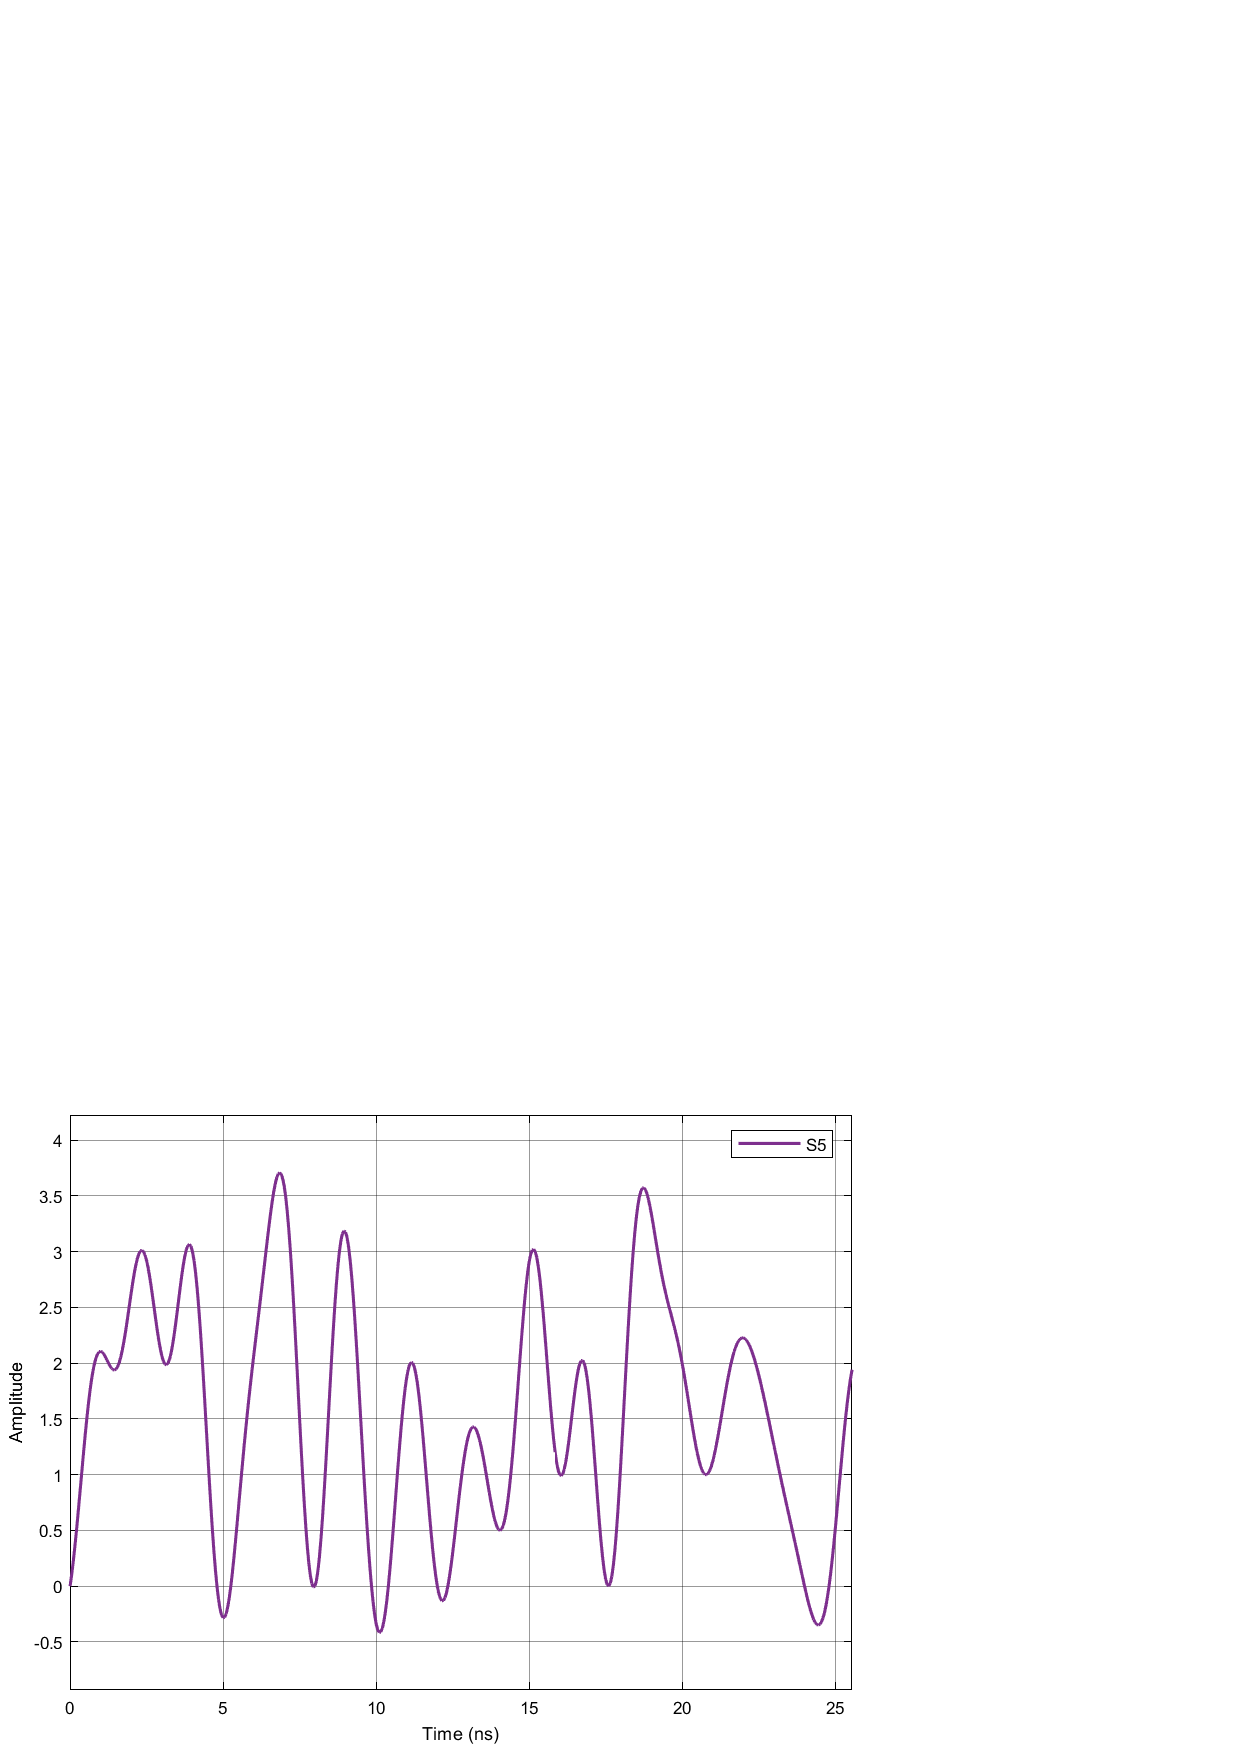
\includegraphics[width=0.9\textwidth, height=9cm]{./sdf/simplified_coherent_receiver/figures/S5.png}
	\caption{S5}\label{}
\end{figure}

\begin{figure}[h]
	\centering
	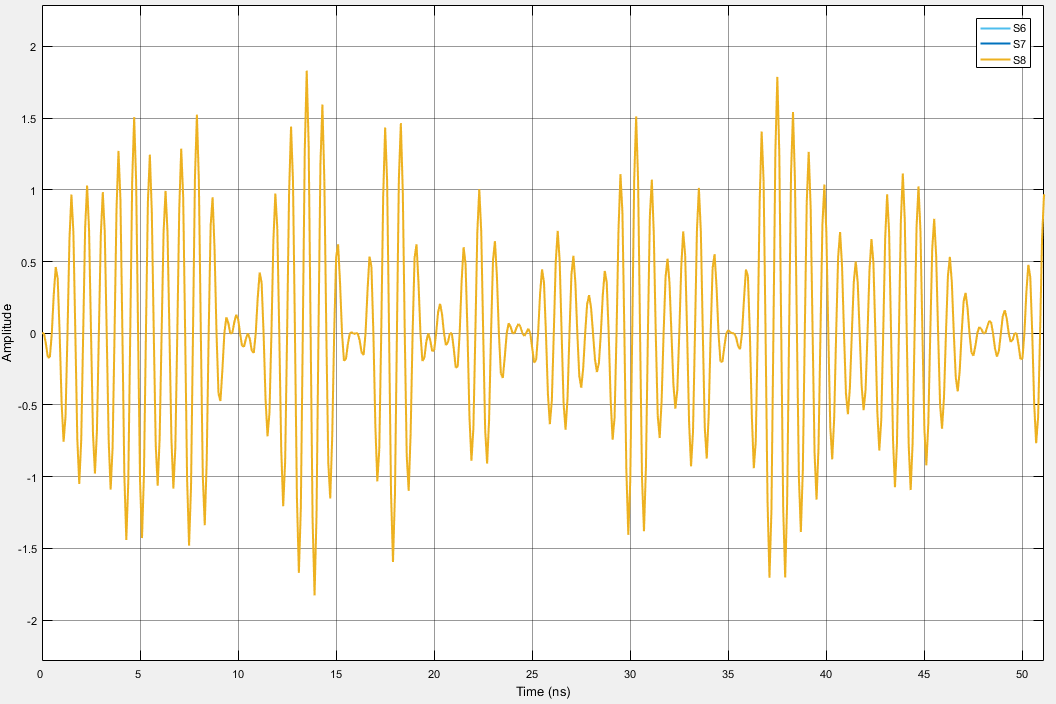
\includegraphics[width=0.9\textwidth, height=9cm]{./sdf/simplified_coherent_receiver/figures/S6S7S8.png}
	\caption{S6, S7 and S8}\label{}
\end{figure}

\begin{figure}[h]
	\centering
	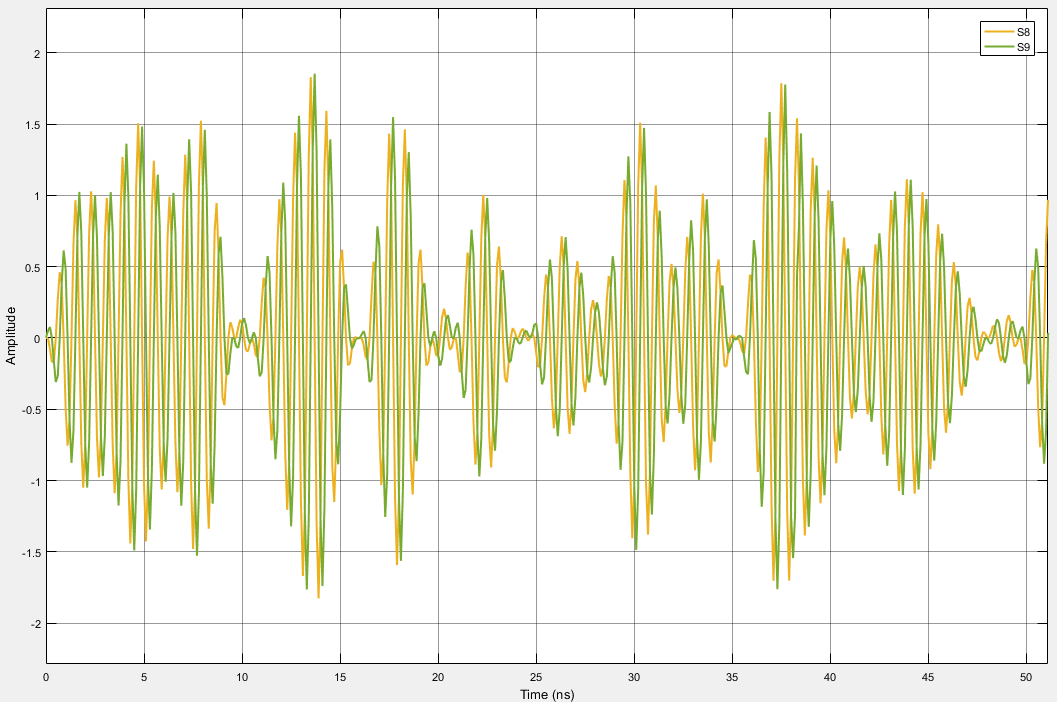
\includegraphics[width=0.9\textwidth, height=9cm]{./sdf/simplified_coherent_receiver/figures/S8S9.png}
	\caption{S8 and S9}\label{}
\end{figure}

\subsubsection{Receiver setup}
\begin{figure}[h]
	\centering
	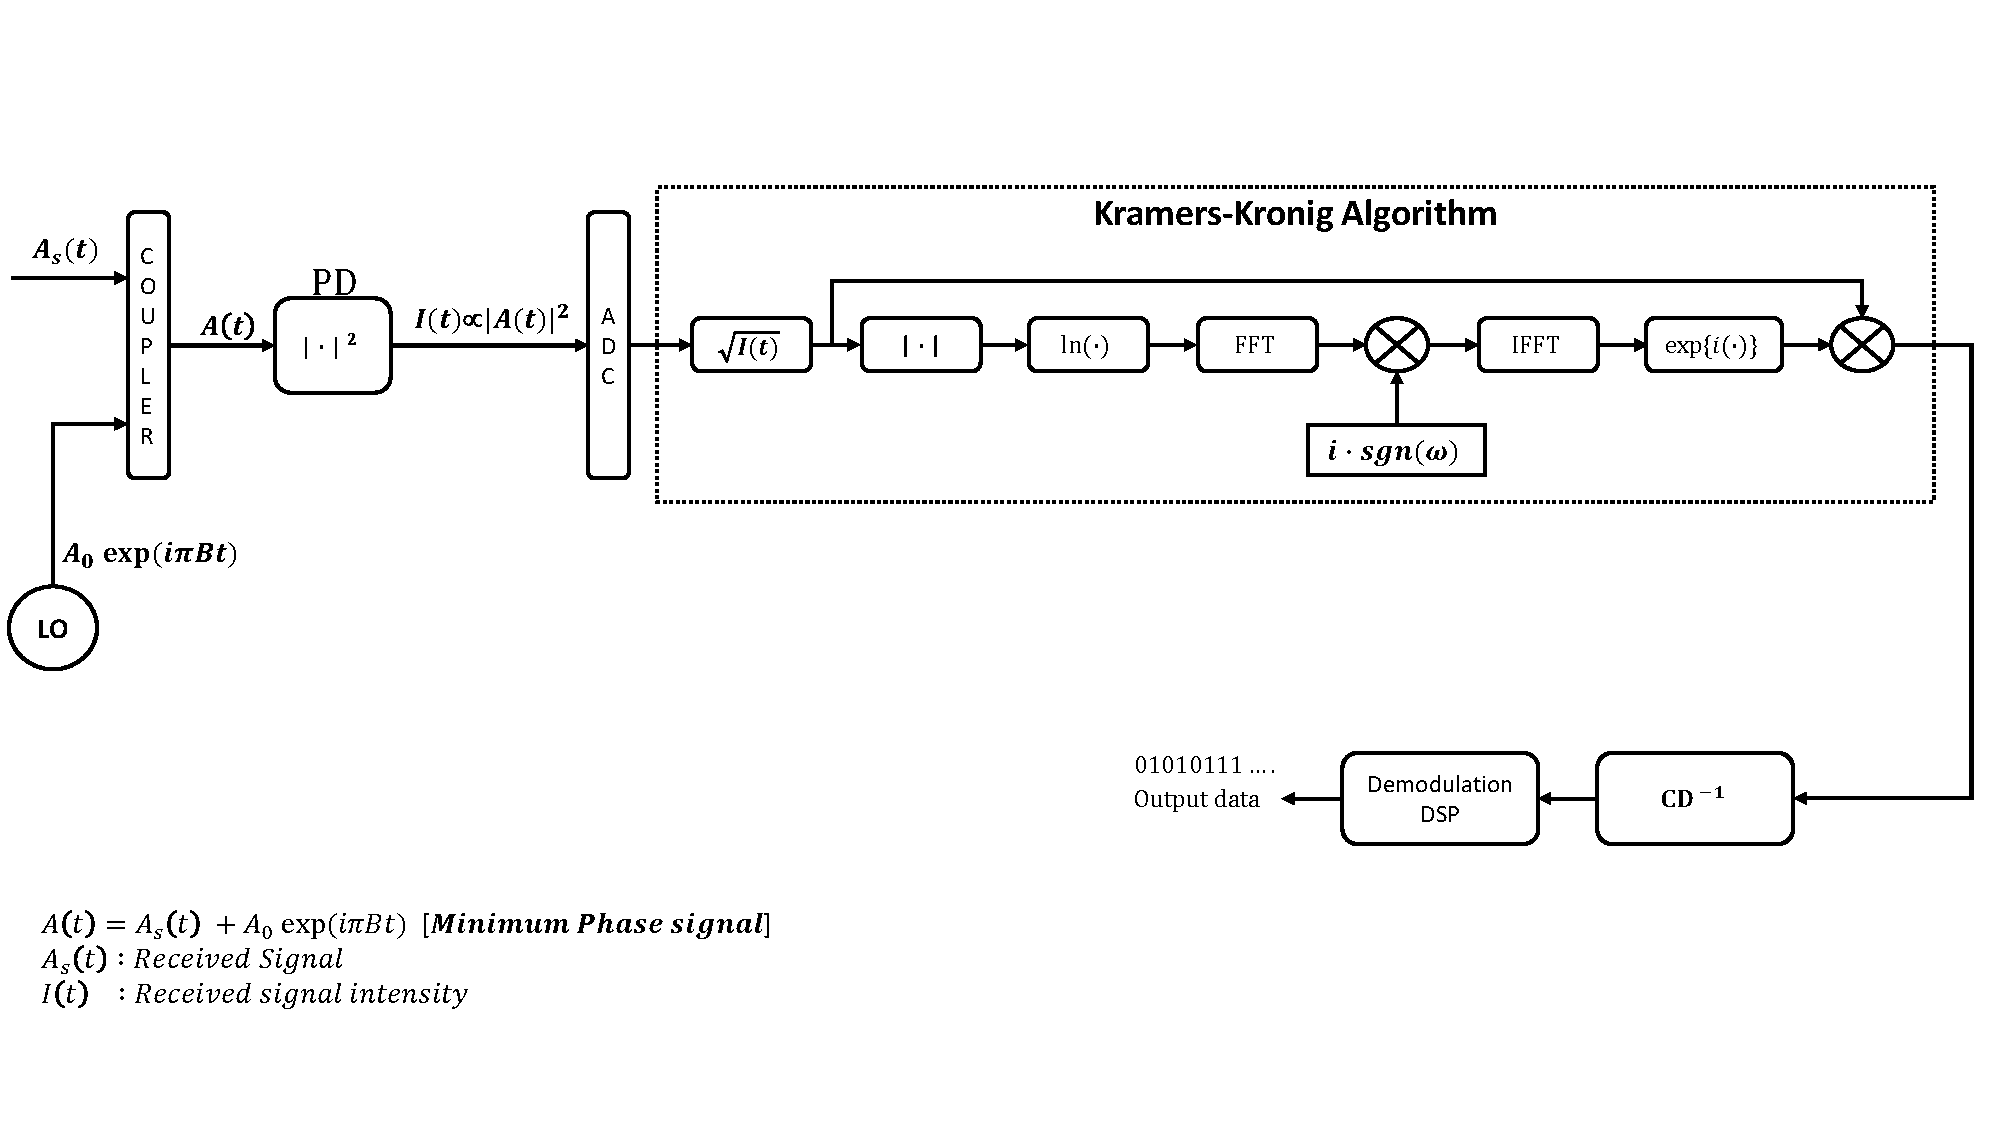
\includegraphics[width=1.0\textwidth, height=10cm]{./sdf/simplified_coherent_receiver/figures/Simulation_setup_Rx.pdf}
	\caption{Receiver simulation setup}\label{Simulation_setup_Rx}
\end{figure}
\newpage
\subsection{Experimental Analysis}
 As shown in the Figure \ref{Practical_setup_TxRx}, at the transmitter end, analytical signal generated with the help of netxpto and applied to the AWG. Waveform generated by AWG applied dual polarization IQ modulator which generates SSB signal in optical domain. SSB optical signal generated by both the IQ modulator is then combined using polarization beam combiner (PBC) and launched into the optical fiber.\\
 At the receiver end, the PDM received signal first spitted by a polarization beam splitter (PBS). Each polarization is combined with an LO tapped from the transmit laser. The laser's wavelength and power are set to ensure that the received signal should satisfy the minimum phase condition. After direct-detection, Kramers-Kronig algorithm is performed on each polarization separately to recover full complex signal. After compensation of the chromatic dispersion, stokes parameter based poldemux algrithm can be applied to recover PDM signals.     
\begin{figure}[h]
	\centering
	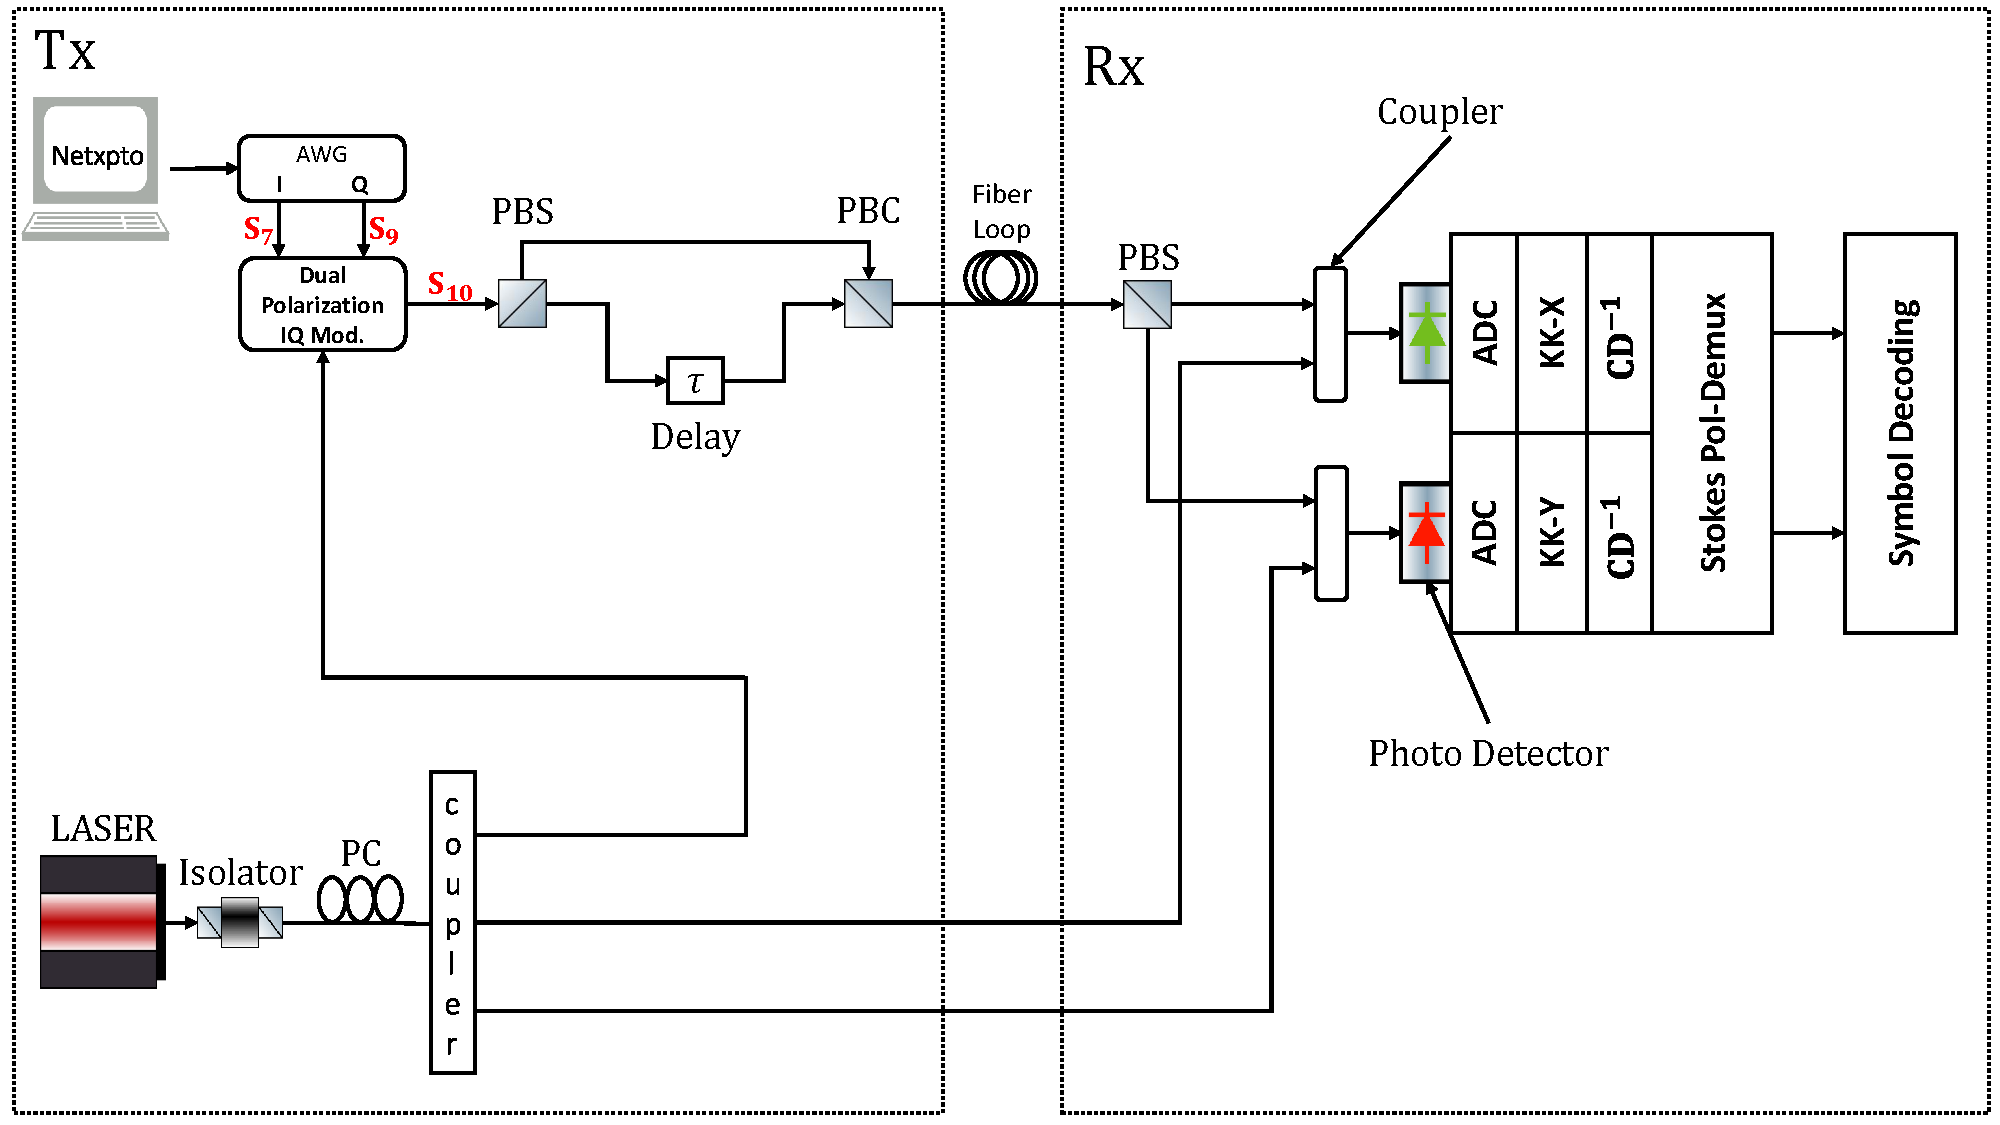
\includegraphics[width=1.0\textwidth, height=7cm]{./sdf/simplified_coherent_receiver/figures/Practical_setup_TxRx.pdf}
	\caption{PDM Kramers-Kronig receiver experimental setup}\label{Practical_setup_TxRx}
\end{figure}

\subsubsection{Status of equipment}
\begin{center}
	\begin{tabular}{ |p{6cm}||p{6.5cm}|p{1.5cm}|   }
		\hline
		%\multicolumn{3}{|c|}{\textbf{Source Files}} \\
		%\hline
		\textbf{Equipment name} & \textbf{Description}&\textbf{Status}\\
		\hline
		LASER				   				&  &\checkmark\\
		\hline
		PC	 								&  &\checkmark\\
		\hline
		Coupler							    &  &\checkmark\\
		\hline
		AWG									&  &\checkmark\\
		\hline
		Dual polarization IQ mod			&  &\checkmark\\
		\hline
		PBS				 					&  &\checkmark\\
		\hline
		PLC									&  &\checkmark\\
		\hline
		Delay								&  &\checkmark\\
		\hline
		Fiber loop							&  &\checkmark\\
		\hline
		Single photodetector				& APD+TIA Optical Receiver:\newline
											  - Maximum bit rate: 10 Gb/s\newline
											  - Sensitivity: -26 dBm &\checkmark\\
		\hline
	\end{tabular}
\end{center}

\subsection{Comparative Analysis}

\subsection{Know Problems}

\begin{center}
	\begin{tabular}{ |p{6cm}||p{6.5cm}|p{1.5cm}|   }
		\hline
		%\multicolumn{3}{|c|}{\textbf{Source Files}} \\
		%\hline
		\textbf{Problem type} & \textbf{Description}&\textbf{Note}\\
		\hline
		Simulator			& Require a generalized block for FFT and IFFT  &DONE!\\
		\hline
	\end{tabular}
\end{center}


\begin{thebibliography}{9}
	\bibitem{latexcompanion}
	Antonio Mecozzi, Cristian Antonelli, and Mark Shtaif.
	\textit{Kramers-Kronig Coherent Receiver}.
	Optica, vol.3, no.11, 2016, p.1220., doi:10.1364/optica.3.001220.
	
	\bibitem{latexcompanion}
	Antonio Mecozzi.
	\textit{Retrieving the full optical response from amplitude data by Hilbert transform}. Opt. Comm. 282, 4183-4187.
	
	\bibitem{latexcompanion}
	Antonio Mecozzi.
	\textit{A necessary and sufficient condition for minimum phase and implication of phase retrieval}. arXiv:1606.04861.
\end{thebibliography}

\subsubsection{\textbf{APPENDICES}}
%%%%%%%%%%%%%%%%%%%%%%%%%%%%%%%%%%%%%%%%%%%%%%%%%%%%%%%%%%%%%%%%%%%%%%%%%%%%%%%%%%%%%%%%%%%%%%%%%%%%%%%%%%
\textbf{Appendix A : SSB with graphical explanation}\\
This section describes the SSB signal generation using Hilbert transformation method (Phase Shift Method). Consider a message signal $m(t)$ with its frequency domain spectrum $M(F)$ as shown in Figure\ref{Original_baseband_signal}. From the Figure \ref{Original_baseband_signal}, we can see that both the side are scaled by factor '1' which means it represents the original signal.
\begin{figure}[h]
	\centering
	\includegraphics[width=0.6\textwidth, height=5cm]{./sdf/simplified_coherent_receiver/figures/SSB1.pdf}
	\caption{Original baseband signal}\label{Original_baseband_signal}
\end{figure}\\ 	
Now let's consider the modulated signal $x(t)$ given as,
\begin{equation}
x(t)=m(t) cos(2\pi f_c t)
\label{Eq:5.20}
\end{equation}
Frequency domain representation of the equation \ref{Eq:5.20} can be given as,
\begin{equation}
X(F)=\frac{1}{2}M(f-f_c)+\frac{1}{2}M(f+f_c)
\label{Eq:5.21}
\end{equation}
Here in equation \ref{Eq:5.21}, we can observe that each side band are scaled by $\dfrac{1}{2}$ on the frequency spectrum. Figure displays the frequency domain representation of the modulated signal $X(F)$.
\begin{figure}[h]
	\centering
	\includegraphics[width=1.0\textwidth, height=8cm]{./sdf/simplified_coherent_receiver/figures/SSB2.pdf}
	\caption{Original modulated signal}\label{Original_modulated_signal}
\end{figure}\\ 
Next, we will discuss something more interesting which is called as Hilbert transform of the original message signal $m(t)$. As we discussed earlier, in the frequency domain, the Hilbert transformed signal $\hat{M}(f)$ can be achieved by multiplying the Fourier transformed signal $M(F)$ with $[-i sgn(F)]$.
\begin{figure}[h]
	\centering
	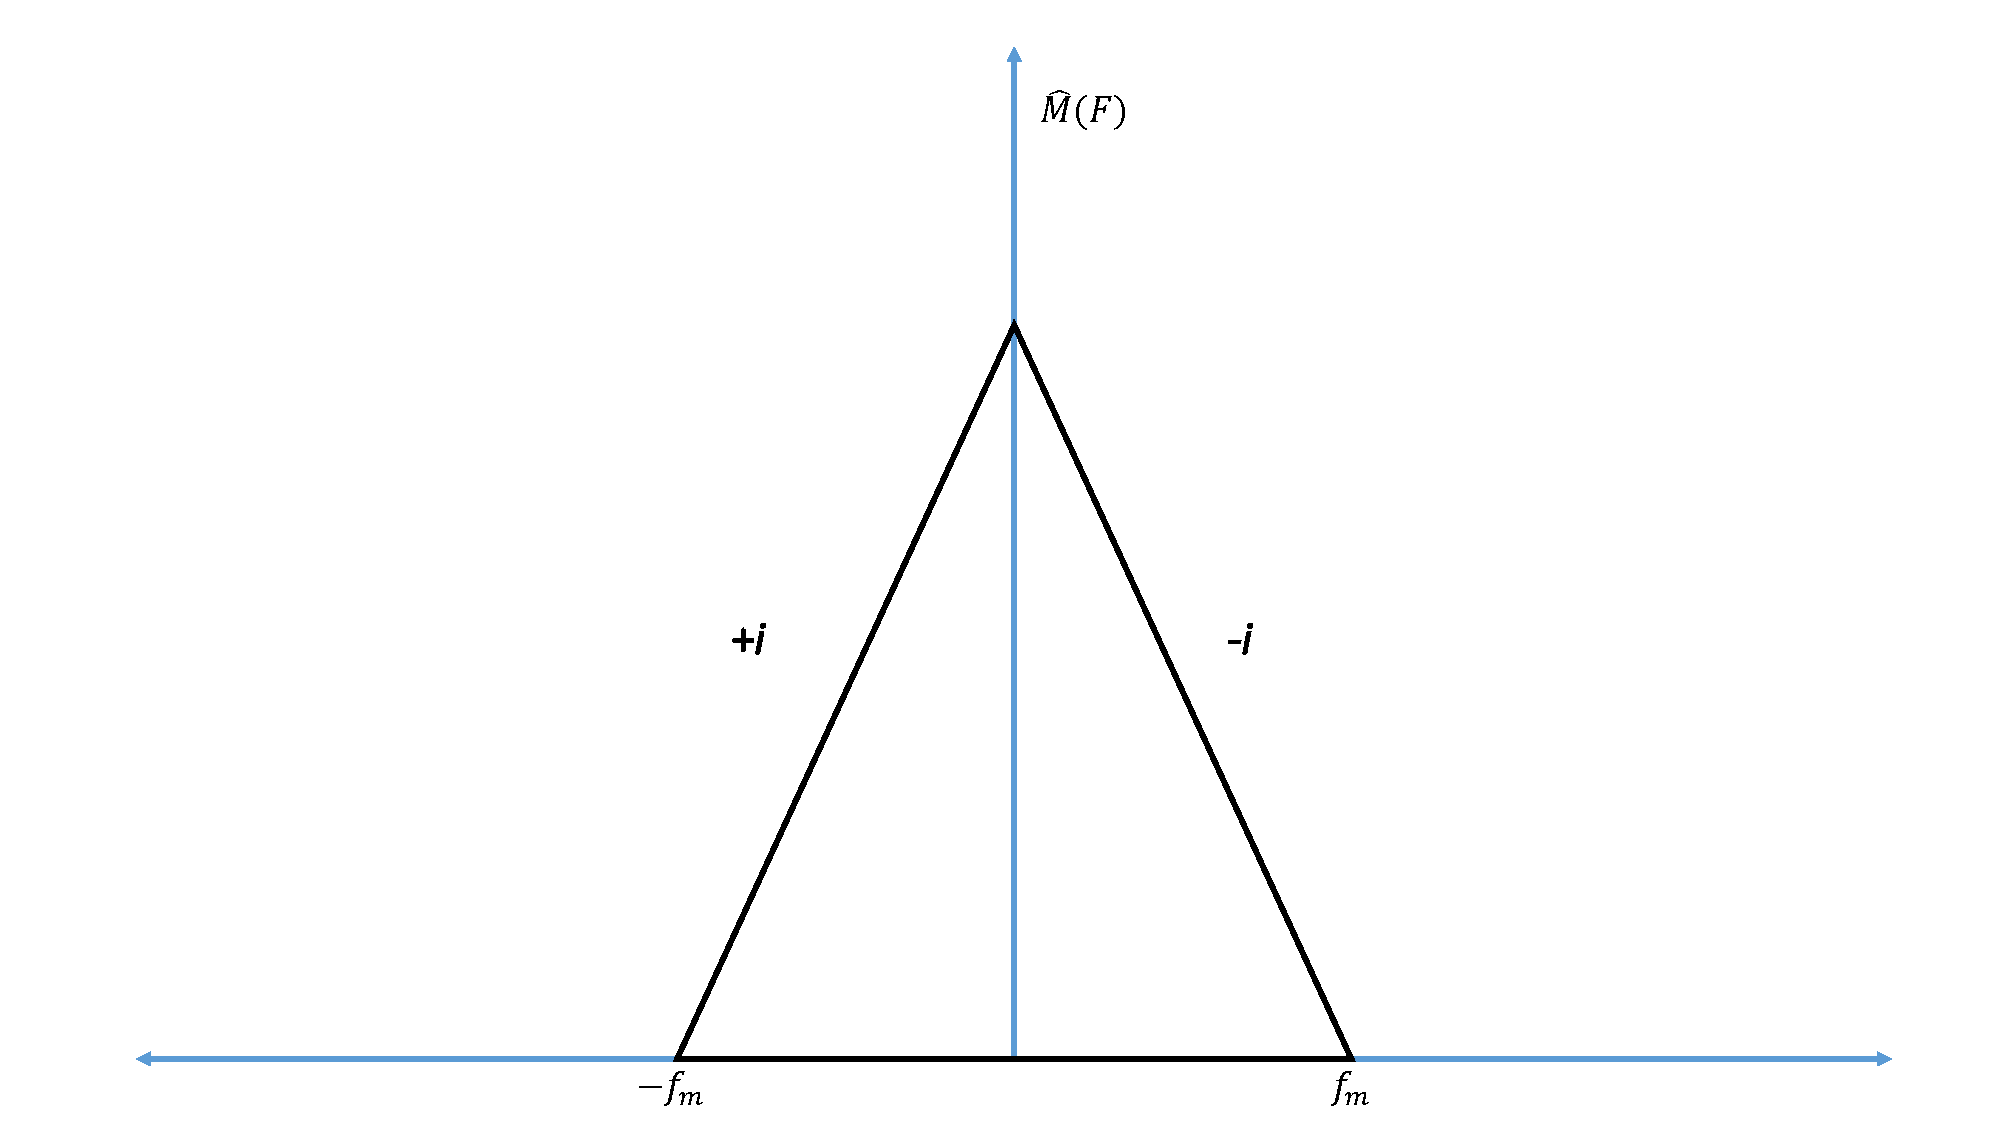
\includegraphics[width=0.6\textwidth, height=5cm]{./sdf/simplified_coherent_receiver/figures/SSB3.pdf}
	\caption{Hilbert transformed modulated signal}\label{Hilbert_Transformed_signal}
\end{figure}
Suppose we modulate the Hilbert transformed message signal $\hat{m}(t)$  with the $sin(2\pi f_c t)$ (quadrature phase carrier), then we get the following results:

\begin{equation}
\begin{split}
{\hat{m}(t)} sin(2\pi f_c t)&={\hat{m}(t)}\frac{e^{i2\pi f_c t} - e^{-i2\pi f_c t} }{2}\\
&={\hat{m}(t)}\frac{e^{i2\pi f_c t}}{2} - {\hat{m}(t)}\frac{e^{-i2\pi f_c t}}{2}\\
&={\frac{\hat{M}(f-f_c)}{2i}}-{\frac{\hat{M}(f+f_c)}{2i}}\\
&={\frac{-i}{2}\hat{M}(f-f_c)}+{\frac{-i}{2}\hat{M}(f+f_c)}\\
\end{split}
\label{Eq:5.46}
\end{equation}
The detailed explanation of the equation \ref{Eq:5.46} has been given in the Figure \ref{Hilbert_Transformed_modulated_signal} and \ref{Hilbert_Final}. Figure \ref{Hilbert_Transformed_modulated_signal} displays the spectrum of the $\hat{M}(f+f_c)$ and $\hat{M}(f-f_c)$ for the positive and negative frequencies respectively. The final equation resolution of equation displays that both positive and negative side of the spectrum multiplied with $\frac{i}{2}$ and $\frac{-i}{2}$ respectively. Finally the spectrum of the signal ${\hat{m}(t)} sin(2\pi f_c t)$ can be given as Figure \ref{Hilbert_Final}.
\begin{figure}[h]
	\centering
	\includegraphics[width=1.0\textwidth, height=8cm]{./sdf/simplified_coherent_receiver/figures/SSB4.pdf}
	\caption{Hilbert transformed modulated signal}\label{Hilbert_Transformed_modulated_signal}
\end{figure}

\begin{figure}[h]
	\centering
	\includegraphics[width=1.0\textwidth, height=8cm]{./sdf/simplified_coherent_receiver/figures/SSB5.pdf}
	\caption{Hilbert transformed modulated signal}\label{Hilbert_Final}
\end{figure}

Further, summation of the two signals ${m(t)} cos(2\pi f_c t)$ and ${\hat{m}(t)} sin(2\pi f_c t)$ will generate the upper sideband SSB signal as follows,
\begin{equation}
u(t)={m(t)} cos(2\pi f_c t)-{\hat{m}(t)} sin(2\pi f_c t)
\label{5.23}
\end{equation}
From the above discussion, the spectrum of the Equation \ref{5.23} can be given by the Figure \ref{SSB_signal_spectrum}. Similarly, for the lower sideband SSB can be generated by Equation,
\begin{equation}
u(t)={m(t)} cos(2\pi f_c t)+{\hat{m}(t)} sin(2\pi f_c t)
\label{5.24}
\end{equation}
\begin{figure}[h]
	\centering
	\includegraphics[width=1.0\textwidth, height=8cm]{./sdf/simplified_coherent_receiver/figures/SSB6.pdf}
	\caption{SSB signal spectrum}\label{SSB_signal_spectrum}
\end{figure}
%%%%%%%%%%%%%%%%%%%%%%%%%%%%%%%%%%%%%%%%%%%%%%%%%%%%%%%%%%%%%%%%%%%%%%%%%%%%%%%%%%%%%%%%%%%%%%%%%%%%%%%%%%
\textbf{Appendix B : Kramers-Kronig scheme}\\
If we consider the complex envelope of the incoming electric field by $A_s(t)$ confined within the optical bandwidth denoted by B. The LO assumed to be a continuous wave (CW) signal whose amplitude is $A_0$ whose frequency coincides with the left edge of the information-carrying signal spectrum. Here, we assumed that $A_0$ is real-valued and positive, which is equivalent to referring all phase value to that of LO.\\
The complex envelope of the field striking upon the photo-diode can be given as,
\begin{equation}
A(t)=A_s(t)+A_0 exp(i\pi Bt)
\end{equation}
The photo current $I$ produced by the photo-diode is proportional to the field intensity $I=|A(t)|^2$, here proportionality constant considered as 1 for the sake of simplicity. If $A_0$ is large enough to ensure that the signal $A(t)exp(-i\pi Bt)=A_0+A_s(t)exp(-i\pi Bt)$ is minimum phase. The discussed hypothesis can be used to reconstruct the signal $E_s(t)$ as follows[1]:
\begin{equation}
A_s(t)=\{\sqrt{I(t)} exp[i\phi_E(t)]-A_0\} exp(i\pi Bt)
\end{equation}
\begin{equation}
\phi_A(t)=\dfrac{1}{2\pi} p.v. \int_{-\infty}^{\infty} dt' \frac{log[|I(t')|]}{t-t'}
\label{Eq:5.19}
\end{equation}
 \fi
\ifdefined\dsp          \input{./sdf/dsp_laser_phase_compensation/dsp_laser_phase_compensation} \fi
\ifdefined\quantumRNG   \clearpage
\section{Quantum Random Number Generator}

\begin{refsection}

\begin{tcolorbox}	
\begin{tabular}{p{2.75cm} p{0.2cm} p{10.5cm}} 	
\textbf{Students Name}  &:& Mariana Ramos (12/01/2018 - 11/04/2018)\\
\textbf{Goal}          &:& Simulate and implement an experimental setup of a Quantum Random Number Generator.\\
\textbf{Directory}          &:& sdf/quantum\_random\_number\_generator.
\end{tabular}
\end{tcolorbox}

True random numbers are indispensable in the field of cryptography \cite{Katsoprinakis08}. There are two approaches for random number generation: the pseudorandom generation which are based on an algorithm implemented on a computer, and the physical random generators which consist in measuring some physical observable with random behaviour. Since classical physics description is deterministic, all classical processes are in principle predictable. Therefore, a true random number generator must be based on a quantum process \cite{Jennewein00}.

In this chapter, it is presented the theoretical, the simulation and the experimental analysis of a quantum random generator based on the use of single photons linearly polarized at $45^{\circ}$.

\subsection{Theoretical Analysis}

One of the optical processes available as a source of randomness is the splitting of a polarized single photon beam. The principle of operation of the random generator is shown in figure \ref{qrng}. Each individual photon coming from the source is linearly polarized at $45^\circ$ and has equal probability of be found in the horizontal (H) or in the vertical (V) output of the PBS. Quantum theory estimates for both cases that the individual choices are truly random, independent one from each other , and with a probability of 1/2.

\begin{figure}[H]
    \centering
        \includegraphics[clip, trim=3cm 20cm 5cm 5cm, width=1.00\textwidth]{./sdf/quantum_random_number_generator/figures/Random_Number_Generator.pdf}
    \caption{Source of randomness with a polarization beam splitter PBS where the incoming light is linearly polarized at $45^{\circ}$ with respect to the PBS. Figure adapted from \cite{Jennewein00}.}\label{qrng}
\end{figure}

From a classical approach, the information is stored as binary bits that can take the logical value '0' or '1'. From a quantum approach, the information can be stored in quantum bits or qubits for short. As a consequence of the superposition principle of quantum mechanics, qubits can not only represent the pure '0' or '1' states, but they can also represent a superposition of both. This way, qubits are governed by a quantum wave function $\psi$. Lets use the Dirac notation to represent the general state of the qubit:
\begin{equation}\label{eq:qubit}
  |\psi\rangle = C_0 |0\rangle + C_1 |1\rangle,
\end{equation}

and the normalization condition of $|\psi\rangle$ requires that $|C_0|^2+|C_1|^2=1$. This way, the relative proportion of each of the binary states on a qubit is governed by the amplitude coefficients $C_0$ and $C_1$. In the present example, we consider a linear polarization in which the two possible states are orthogonal, such that: $\langle 0|1 \rangle=0$. We define the $|0\rangle$ and $|1\rangle$ states to correspond to the horizontal and vertical polarization states, respectively:

\begin{eqnarray}
 %\nonumber % Remove numbering (before each equation)
  |\psi\rangle &=& C_0 |0\rangle+C_1 |1\rangle \\
             &=& C_0 |0^{\circ}\rangle + C_1 |90^{\circ}\rangle .
\end{eqnarray}

Amplitude coefficients $C_0$ and $C_1$ store the quantum information. Therefore, if one makes a measurement, the result will be '0' with probability $|C_0|^2$ or '1' with probability $|C_1|^2$.
Moreover, the state of a single photon can be also described by a wave function as a column vector:

\begin{equation}\label{eq:wavefvector}
  |\psi\rangle = \binom{C_0}{C_1},
\end{equation}
which will be used in simulation analysis.

\begin{figure}[h]
    \centering
        \includegraphics[clip, trim=3cm 20cm 12cm 3cm, height=6cm]{./sdf/quantum_random_number_generator/figures/axis_states.pdf}
    \caption{Representation of polarization states of a qubit in a bi-dimensional space.}\label{fig:stateaxis}
\end{figure}

As one can see in figure \ref{fig:stateaxis} the amplitude coefficients can be written as a function of $\theta$:
\begin{eqnarray}
% \nonumber % Remove numbering (before each equation)
  C_0 &=& cos(\theta) \\
  C_1 &=& sin(\theta).
\end{eqnarray}

According with the setup presented in figure \ref{qrng} and considering the polarization angle $\theta = 45^{\circ}$, the single photon has the probability of reach \textbf{D1} and outputs a "$0$" is equals to $|cos(\theta)|^2$ and the probability of reach \textbf{D2} and outputs a "$1$" is equals to $|sin(\theta)|^2$, which in the case $\theta = 45^{\circ}$ both have the same value equals to $0.5$.

\subsection{Simulation Analysis}
The simulation diagram of the setup described in the previous section is presented in figure \ref{sim_qrng}. The linear polarizer has an input control signal (S1) which allows to change the rotation angle. Nevertheless, the only purpose is to generate a time and amplitude continuous real signal with the value of the rotation angle in degrees. In addition, the photons are generated by single photon source block at a rate defined by the clock rate. At the end of the simulation there is a circuit decision block which will outputs a binary signal with value "$0$" \space if the detector at the end of the horizontal path clicks or "$1$" \space if the detector at the end of the vertical path clicks.

\begin{figure}[h]
    \centering
        \includegraphics[clip, trim=5cm 5cm 0.5cm 15cm, width=1.00\textwidth]{./sdf/quantum_random_number_generator/figures/Simulation_qrng.pdf}
    \caption{Block diagram of the simulation of a Quantum Random Generator.}\label{sim_qrng}
\end{figure}

In table \ref{tb:inputparameters2} are presented the input parameters of the system.


\begin{table}[H]
\centering
\caption{System Input Parameters}
\label{tb:inputparameters2}
\begin{tabular}{|c|c|c|}
\hline
\textbf{Parameter}                      & \textbf{Default Value}                                       \\ \hline
RateOfPhotons                           & 1e6                                                          \\ \hline
NumberOfSamplesPerSymbol                & 16                                                           \\ \hline
PolarizerAngle                          & 45.0                                                         \\ \hline

\end{tabular}
\end{table}

In table \ref{tb:signals2} are presented the system signals to implement the simulation presented in figure \ref{sim_qrng}.
\begin{table}[H]
\centering
\caption{System Signals}
\label{tb:signals2}
\begin{tabular}{|c|c|c|}
\hline
\textbf{Signal name}                            & \textbf{Signal type}                      \\ \hline
S1                                              &  TimeContinuousAmplitudeContinuousReal    \\ \hline
S2                                              &  TimeContinuousAmplitudeContinuousReal    \\ \hline
S3                                              &  PhotonStreamXY                           \\ \hline
S4                                              &  PhotonStreamXY                           \\ \hline
S5                                              &  PhotonStreamXYMP                         \\ \hline
S6                                              &  TimeContinuousAmplitudeContinuousReal    \\ \hline
S7                                              &  TimeContinuousAmplitudeContinuousReal    \\ \hline
S8                                              &  Binary                                   \\ \hline
S9                                              &  Binary                                   \\ \hline
\end{tabular}
\end{table}

Table \ref{tb:signalsh} presents the header files used to implement the simulation as well as the specific parameters that should be set in each block. Finally, table \ref{tb:signalss} presents the source files.

\begin{table}[H]
\centering
\caption{Header Files}
\label{tb:signalsh}
\begin{tabular}{|c|c|c|}
\hline
\textbf{File name}                              & \textbf{Description}                                                          & \textbf{Status} \\ \hline
netxpto\_20180118.h                             &                                                                               &    \checkmark   \\ \hline
electrical\_signal\_generator\_20180124.h       &setFunction(), setGain()                                                       &    \checkmark   \\ \hline
clock\_20171219.h                               &ClockPeriod(1 / RateOfPhotons)                                                 &    \checkmark   \\ \hline
polarization\_beam\_splitter\_20180109.h        &                                                                               &   \checkmark   \\ \hline
polarizer\_20180113.h                           &                                                                               &    \checkmark   \\ \hline
single\_photon\_detector\_20180111.h            &setPath(0), setPath(1)                                                         &    \checkmark   \\ \hline
single\_photon\_source\_20171218.h              &                                                                               &    \checkmark   \\ \hline
probability\_estimator\_20180124.h              &                                                                               &    \checkmark   \\ \hline
sink.h                                          &                                                                               &    \checkmark   \\ \hline
qrng\_decision\_circuit.h                       &                                                                               &    \checkmark   \\ \hline
\end{tabular}
\end{table}

\begin{table}[H]
\centering
\caption{Source Files}
\label{tb:signalss}
\begin{tabular}{|c|c|c|}
\hline
\textbf{File name}                              & \textbf{Description} & \textbf{Status} \\ \hline
netxpto\_20180118.cpp                           &                      &    \checkmark   \\ \hline
electrical\_signal\_generator\_20180124.cpp     &                      &    \checkmark   \\ \hline
clock\_20171219.cpp                             &                      &    \checkmark   \\ \hline
polarization\_beam\_splitter\_20180109.cpp      &                      &   \checkmark   \\ \hline
polarizer\_20180113.cpp                         &                      &    \checkmark   \\ \hline
single\_photon\_detector\_20180111.cpp          &                      &    \checkmark   \\ \hline
single\_photon\_source\_20171218.cpp            &                      &    \checkmark   \\ \hline
probability\_estimator\_20180124.cpp            &                      &    \checkmark   \\ \hline
sink.cpp                                        &                      &    \checkmark   \\ \hline
qrng\_decision\_circuit.cpp                     &                      &    \checkmark   \\ \hline
qrng\_sdf.cpp                                   &                      &    \checkmark   \\ \hline
\end{tabular}
\end{table}

 Lets assume, for an angle of $45^{\circ}$, a number of samples$N=1 \times 10^{6}$ and the expected probability of reach each detector of $\hat{p} = 0.5$. We have an error margin of $E = 1.288 \times 10 ^{-3}$, which is acceptable. This way, the simulation will be performed for $N=1 \times 10^{6}$ samples for different angles of polarization shown in figure \ref{sphere} with different error margin's values since the expected probability changes depending on the polarization angle.

\begin{figure}[H]
    \centering
        \includegraphics[clip, trim=0.5cm 15.5cm 2.5cm 1cm, height = 10cm]{./sdf/quantum_random_number_generator/figures/sphere.pdf}
    \caption{Angles used to perform the qrng simulation for $N=1 \times 10^{6}$ samples. }\label{sphere}
\end{figure}

For a quantum random number generator with equal probability of obtain a "0" \space or "1" \space the polarizer must be set at $45^{\circ}$. This way, we have $50\%$ possibilities to obtain a "0" \space and $50\%$ of possibilities to obtain a "1" \space. This theoretical value meets the value obtained from the simulation when it is performed for the number of samples mentioned above.

\begin{figure}[H]
    \centering
        \includegraphics[width=15cm,height=10cm]{./sdf/quantum_random_number_generator/figures/prob0.eps}
    \caption{Probability of outputs a number "0" \space depending on the polarization angle.}\label{probx}
\end{figure}

Figure \ref{probx} shows the probability of a single photons reaches the detector placed on Horizontal axis depending on the polarization angle of the photon, and this way the output number is "0". The following table shows the goodness of the fit:
\begin{table}[H]
\centering
\label{tab:goodnessfitprob0}
    \begin{tabular}{c|c}
      SSE:                  & 0.0004785\\
      R-square:             &0.9998\\
      Adjusted R-square:    &0.9995\\
      RMSE:                 &0.007734
  \end{tabular}
\end{table}

On the other hand, figure \ref{proby} shows the probability of a single photon reaches the detector placed on Vertical component of the polarization beam splitter, and this way the output number is "1". As we can see in the figures the two detectors have complementary probabilities, i.e the summation of both values must be equals to $1$. One can see that "Probability of $1$" \space behaves almost like a sine function and "Probability of 0" \space behaves almost like a cosine function with a variable angle.

\begin{figure}[H]
    \centering
        \includegraphics[width=15cm,height=10cm]{./sdf/quantum_random_number_generator/figures/prob1.eps}
    \caption{Probability of outputs a number "1" \space depending on the polarization angle.}\label{proby}
\end{figure}

The goodness of the fit presented in figure \ref{proby} is shown in the following table:
\begin{table}[H]
\centering
\label{tab:goodnessfitprob0}
    \begin{tabular}{c|c}
        SSE:                &0.0004785\\
        R-square:           &0.9998\\
        Adjusted R-square:  &0.9995\\
        RMSE:               &0.007734
  \end{tabular}
\end{table}

The goodness of the fit is evaluated based on four parameters:
\begin{enumerate}
  \item The sum of squares due to error (SSE), which measures the total deviation between the fit values and the values that the simulation outputs. This value is calculated from the expression
      \begin{equation}\label{}
        \textrm{SSE} = \sum_{i=1}^{n} w_i(y_{i}-\hat{y_{i}})^2.
        \nonumber
      \end{equation}
      A value of SSE closer to 0 means that the model has a small random error component.

  \item The R-square measures how good the fit in explaining the data.
    \begin{equation}\label{}
    \textrm{R-square} = 1-\frac{\textrm{SSE}}{\textrm{SST}},
    \nonumber
    \end{equation}
    where,
    \begin{equation}\label{}
    \textrm{SST} = \sum_{i=1}^{n} w_i (y_i - \bar{y_i})^2.
      \nonumber
    \end{equation}
    R-square can take a value between 0 and 1. If the value is closer to 1, it means that the fit better explains the total variation in the data around the average.

  \item Degrees of freedom adjusted R-square uses the R-square and adjusts it based on the number of degrees of freedom.
    \begin{equation}\label{}
      \textrm{adjusted R-square} = 1 - \frac{\textrm{SSE}(n-1)}{\textrm{SST}(v)},
      \nonumber
    \end{equation}
    where,
    \begin{equation}\label{}
      v = n - m,
      \nonumber
    \end{equation}
    where n is the number of values in test and m is the number of fitted coefficients estimated from the values in test. A value of adjusted R-square close to 1 is a indicative factor of a good fit.

  \item The root mean square error (RMSE) is also a fit standard error and it can be calculated from:
    \begin{equation}\label{}
      \textrm{RMSE} = \sqrt{\textrm{MSE}},
      \nonumber
    \end{equation}
    where,
    \begin{equation}\label{}
      \textrm{MSE} = \frac{\textrm{SSE}}{v}.
      \nonumber
    \end{equation}

\end{enumerate}

\subsection{Experimental Analysis}

In order to have a real experimental quantum random number generator, a setup shown in figure \ref{experimental_qrng} was built in the lab. To simulate a single photon source we have a CW-Pump laser with $1550$ nm wavelength followed by an interferometer Mach-Zenhder in order to have a pulsed beam. The interferometer has an input signal given by a Pulse Pattern Generator. This device also gives a clock signal for the Single Photon Detector (APD-Avalanche Photodiode) which sets the time during which the window of the detector is open. After the MZM there is a Variable Optical Attenuator (VOA) which reduces the amplitude of each pulse until the probability of one photon per pulse is achieved. Next, there is a polarizer controller followed by a Linear Polarized, which is set at $45^{\circ}$, then a Polarization Beam Splitter (PBS) and finally, one detector at the end of each output of the PBS. The output signals from the detector will be received by a Processing Unit. Regarding to acquired the output of the detectors, there is an oscilloscope capable of record $1 \times 10^{6}$ samples.



\begin{figure}[H]
    \centering
        \includegraphics[clip, trim=0.5cm 7cm 0.5cm 17cm, width=1.00\textwidth]{./sdf/quantum_random_number_generator/figures/experimental_qrng.pdf}
    \caption{Experimental setup to implement a quantum random number generator.}\label{experimental_qrng}
\end{figure}

\subsubsection{IDQuantique detector}
%
The detector used in the laboratory is the Thorlabs PDB 450C. This detector consists of two well-matched photodiodes and a transimpedance amplifier that generates an output voltage (RF OUTPUT) proportional to the difference between the photocurrents of the photodiodes.\\
Additionally, the unit has two monitor outputs (MONITOR+ and MONITOR-) to observe the optical input power level on each photodiode separately.

Since we do not have a single photon source, we must use the Poisson Statistics in order to calculate the best value for a mean of photons per pulse. A weak laser pulse follows a Poissonian Statistics\cite{Fox06}:
\begin{equation}\label{eq:poisson}
  S_n = e^{-\mu}\frac{\mu^{n}}{n!},
\end{equation}
where $\mu$ is the average photon number. In addition, the probability of an optical pulse carries one photon at least is:
\begin{equation}\label{eq:prob1photon}
  P = 1 - S_0 = 1 - e^{-\mu}.
\end{equation}

On the other hand, the probability of a detector clicks is:

\begin{equation}\label{eq:detectorclickprob}
  P_{click} = P_{det}+P_{dc} + P_{det}P_{dc},
\end{equation}

where $P_{det}$ is the probability of the detector clicks due a photon which cross its window and $P_{dc}$ is the probability of dark counts. Considering the detector efficiency $\eta_{D}$, the probability of the detector clicks due to a photon is:

\begin{equation}\label{eq:probclickefficiency}
  P_{det} = 1 - e^{- \eta_{D}\mu}.
\end{equation}

The probability of dark counts is calculated as a ratio between the frequency counts and the trigger frequency when no laser is connected to the detector. Nevertheless, the detector click frequency is
\begin{equation}\label{eq:frequencyclick}
  f_{click} = f_{trigger}P_{click} \longrightarrow P_{click}=\frac{f_{click}}{f_{trigger}}.
\end{equation}

This way the mean average photon number can be calculate using the following equation:
\begin{equation}\label{eq:meanphotonnumber}
  \mu = - \frac{1}{\eta_{D}}\ln\left [1-\frac{1}{1-P_{dc}}\left (\frac{f_{click}}{f_{trigger}}-P_{dc} \right)\right]
\end{equation}

\subsection{Open Issues}
\begin{itemize}
  \item Experimental Implementation.
  \item Random number validation/standardization. 
\end{itemize}
\newpage


% bibliographic references for the section ----------------------------
\clearpage
\printbibliography[heading=subbibliography]
\end{refsection}
\addcontentsline{toc}{subsection}{Bibliography}
\cleardoublepage
% --------------------------------------------------------------------- 
 \fi
\ifdefined\bb           \clearpage
\section{BB84 with Discrete Variables}

\begin{refsection}

\begin{tcolorbox}	
\begin{tabular}{p{2.75cm} p{0.2cm} p{10.5cm}} 	
\textbf{Students Name}  &:& Mariana Ramos (7/11/2017 - 9/4/2018) \\
                        & & Kevin Filipe (7/11/2017 - 10/11/2017) \\
\textbf{Starting Date} &:& November 7, 2017\\
\textbf{Goal}          &:& BB84 implementation with discrete variables.
\end{tabular}
\end{tcolorbox}

BB84 is a key distribution protocol which involves three parties, Alice, Bob and Eve. Alice and Bob exchange information between each other by using a quantum channel and a classical channel. The main goal is continuously build keys only known by Alice and Bob, and guarantee that eavesdropper, Eve, does not gain any information about the keys.


\subsection{Protocol Analysis}
\begin{tcolorbox}	
	\begin{tabular}{p{2.75cm} p{0.2cm} p{10.5cm}} 	
		\textbf{Students Name}  &:& Kevin Filipe (7/11/2017 - 10/11/2017)\\
		\textbf{Goal}          &:& BB84 - Protocol Description
	\end{tabular}
\end{tcolorbox}

BB84 protocol was created by Charles Bennett and Gilles Brassard in 1984 \cite{Bennet84}. It involves two parties, Alice and Bob, sharing keys through a quantum channel in which could be accessed by a eavesdropper, Eve. A basic model is depicted in figure \ref{fig:qkd model}.

\begin{figure}[H]
	\centering
	\includegraphics[width=0.8\textwidth,height=7cm]{./sdf/bb84_with_discrete_variables/figures/QKD_Model.png}
	\caption{Basic QKD Model. Alice and Bob are connected by 2 communication channels, a public quantum channel and a authenticated classical channel, with an eavesdropper, Eve (figure adapted from \cite{Gerry05}).}\label{fig:qkd model}
\end{figure}

We are going to analyse the BB84 protocol with bit encoding into photon state polarization. Two non-orthogonal basis are used to encode the information, the rectilinear and diagonal basis, + and x respectively. The following table shows this bit encoding.
\begin{table}[H]
	\centering
	\begin{tabular}{c|c|c}
		 Bit &  \textit{Rectilinear Basis,+} & \textit{Diagonal Basis,$\times$}\\ \hline
		0 &  0$º$ & -45$º$ \\
		1 & 90$º$ & 45$º$\\
	\end{tabular}
\end{table}

The protocol requires the following parameter and it is implemented with the following steps:

\begin{table}[hbt]
	\centering
	\caption{Initial Parameters.}
	\label{tb:param}
	\begin{tabular}{|c|c|}
		\hline
		\textbf{Parameter}  & \textbf{Description} 	   \\ \hline
			$M \times N$    & Scrambling Matrix M by N \\ \hline
			k				& Number of revealed bits for BER calculation \\ \hline
			$\alpha$        & Confidence level 	       \\ \hline
			    A    & B                \\ \hline
	\end{tabular}
\end{table}

\begin{enumerate}
	\item Alice generates two random bit strings. The random string , $R_{A1}$, corresponds to the data to be encoded into photon state polarization. $R_{A2}$ is a random string in which 0 and 1 corresponds to the rectilinear, +, and diagonal, $\times$, respectively.
	
	$$ R_{A1} = \{0,1,1,0,1,0,0,1,1,0,1,1,1,0,0,1,0,0,0,1\}$$
	\begin{eqnarray}
		R_{A2} &=& \{0,0,1,0,1,1,1,0,1,1,1,0,1,0,0,0,1,0,1,0\} \nonumber \\
		&=& \{+,+,\times,+,\times, \times, \times, +,\times, \times, \times,+,\times,+,+,+,\times,+,\times,+\}\nonumber
	\end{eqnarray}
	
	\item Alice transmits a train of photons, $S_{AB}$, obtained by encoding the bits, $R_{A1}$ with the respective photon polarization state $R_{A2}$.
	
	$$S_{AB} = \{\to, \uparrow, \searrow, \to, \searrow, \nearrow, \nearrow, \uparrow, \searrow, \nearrow, \searrow, \uparrow, \searrow, \to, \to, \uparrow, \nearrow, \to, \nearrow, \uparrow\}.$$
	
	\item Bob generates a random string, $R_{B}$, to receive the photon trains with the correspondent basis.
	\begin{eqnarray}
		R_{B} &=& \{0,1,1,1,0,1,0,0,1,1,0,0,1,1,0,0,1,1,0,0\} \nonumber\\
		&=&\{+,\times,\times,\times,+,\times,+,+,\times,\times,+,+,\times,\times,+,+,\times,\times,+,+\} \nonumber
	\end{eqnarray}
	
	\item Bob performs the incoming photon states measurement, $M_{B}$, with its generated random basis, $R_{B}$. If the two photon detectors don't click, means the bit was lost during transference due to attenuation. If both photon detectors click, a false positive was detected. In the measurements, $M_{B}$, the no-click in both detectors is represented by a -1 and the false positives to -2. The measurements done in rectilinear or diagonal basis are represented by 0 or 1, respectively. This is represented \ref{fig:bb84 detector}
	
	$$M_{B} = \{0,1,1,1,-1,1,0,0,-2,1,0,0,-2,1,0,0,1,-1,0,0\}$$	

	\begin{figure}[H]
		\centering
		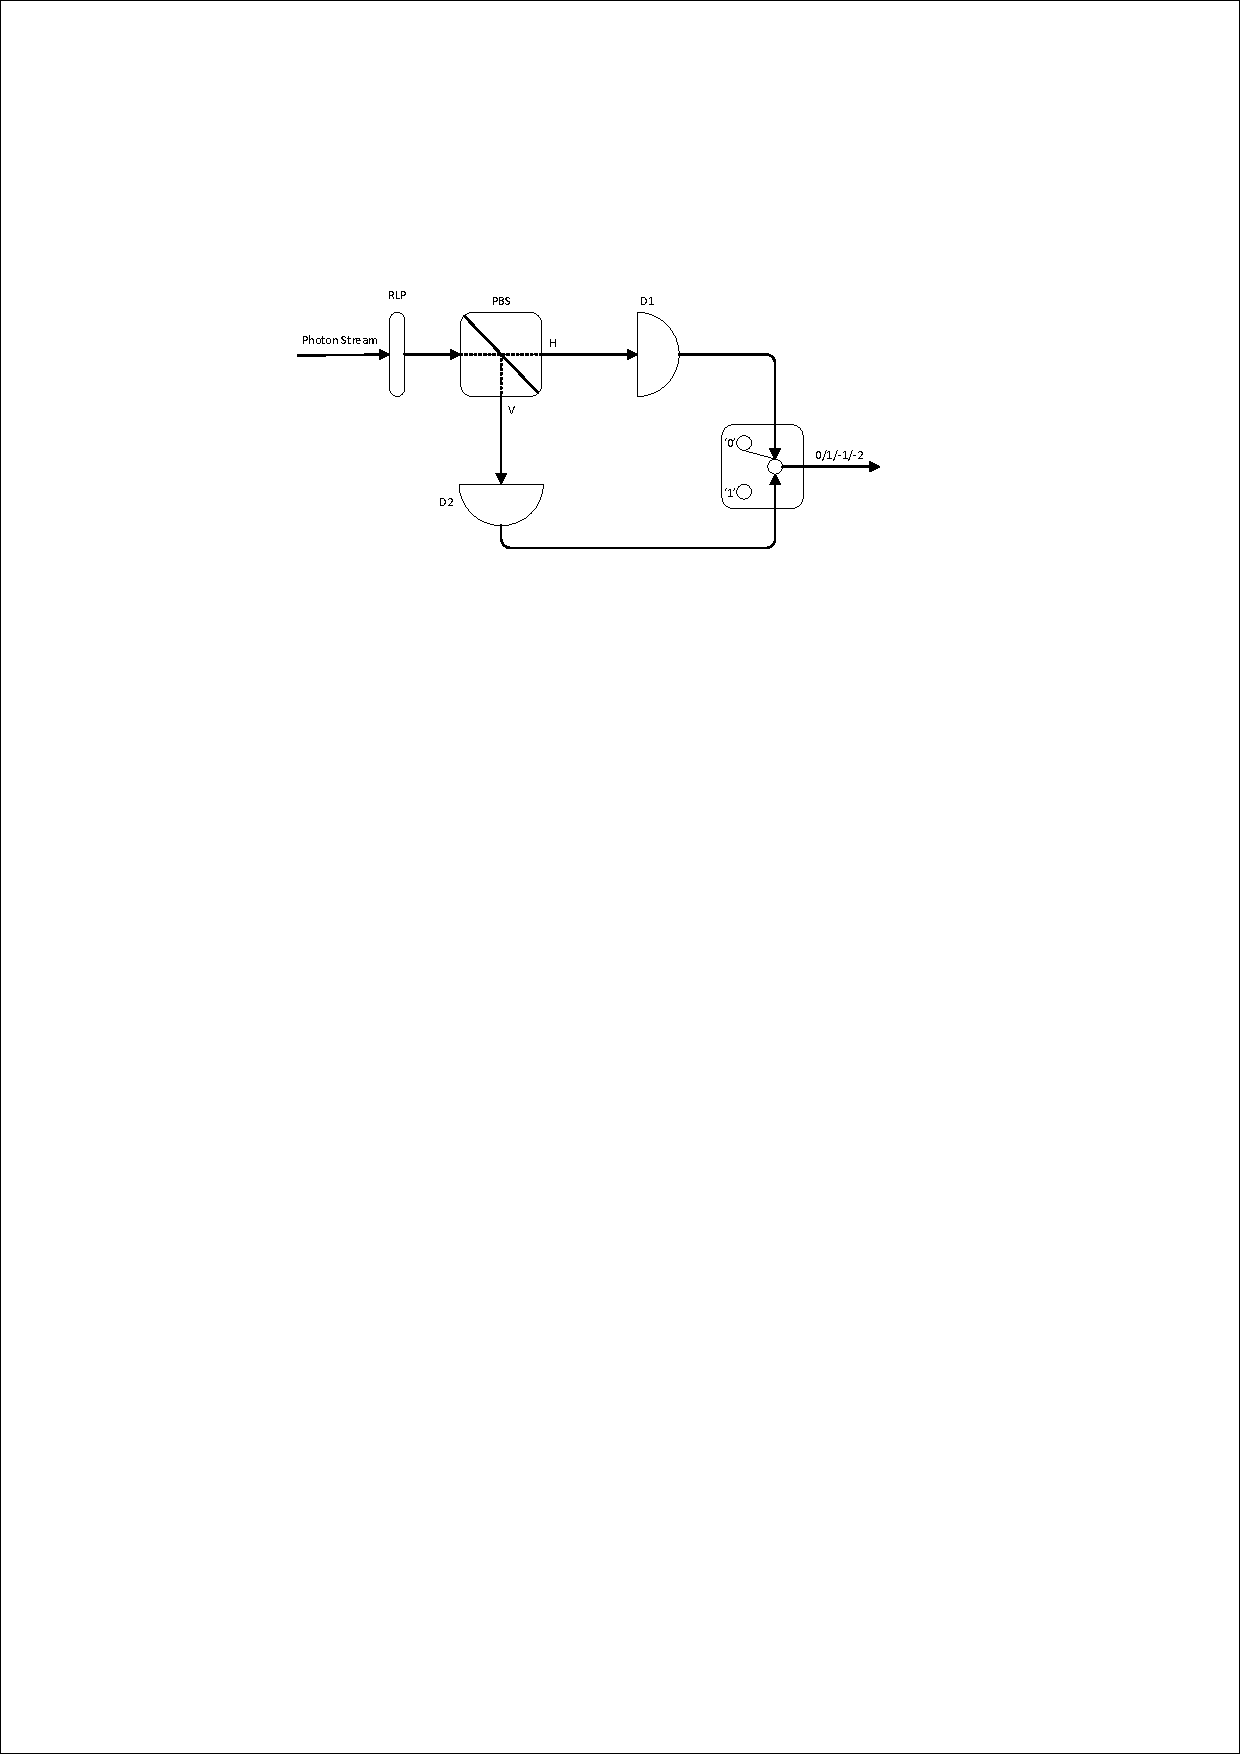
\includegraphics[width=0.8\textwidth,height=7cm]{./sdf/bb84_with_discrete_variables/figures/detector.png}
		\caption{Single-Photon Detection block with false-positives, -2, and attenuation, -1, detection depending on D1 and D2 output.\label{fig:bb84 detector}}
	\end{figure}
	
	\item After the measurement, Bob sends to Alice, using the classical channel, the used basis values, $R_{B}$ with the attenuation, -1, and false positives,-2.
	\item Alice performs a modified negated XOR, generating a sequence that detects when the same basis she used $B_{AB}$.
	
	\begin{table}[H]
		\centering
		\begin{tabular}{c|c c c c c c c c c c c c c c c c c c c c}
			$R_{A2}$ & 0 & 0 & 1 & 0 &  1 & 1 & 1 & 0 &  1 & 1 & 1 & 0 &  1 & 0 & 0 & 0 & 1 &  0 & 1 & 0 \\
			$R_{B}$  & 0 & 1 & 1 & 1 & -1 & 1 & 0 & 0 & -2 & 1 & 0 & 0 & -2 & 1 & 0 & 0 & 1 & -1 & 0 & 0 \\ \hline
			$B_{AB}$ & 1 & 0 & 1 & 0 &  0 & 1 & 0 & 1 &  0 & 1 & 0 & 1 &  0 & 0 & 1 & 1 & 1 &  0 & 0 & 1 \\
		\end{tabular}
	\end{table}

	\item Alice sends the $B_{AB}$ sequence to Bob, in which he can correlate with, $M_{B}$, and deduce the key $K_{AB}$.
	
			$$ K_{AB} = \{0,1,0,1,0,1,0,1,0,1\}.$$
	
	\item Alice then by having knowledge of $R_{A2}$ and $B_{AB}$ performs a scrambling algorithm over the deduced key. It is generated a matrix $M \times N$, according to the input parameter. Assuming a scrambling matrix of 3x4, \ref{tb:scram}. And being the scramble key represented as $KS_{AB}$
	
	\begin{table}[hbt]
		\centering
		\caption{Scrambling matrix}
		\label{tb:scram}
		\begin{tabular}{|c|c|c|c|c|}
			\hline
				0 & 1 & 0 & 1 \\ \hline
			    0 & 1 & 0 & 1 \\ \hline
				0 & 1 & - & - \\ \hline
		\end{tabular}
	\end{table}

	$$KS_{B} = \{0,0,0,1,1,1,0,0,1,1\}$$	
	
	\item Bob uses the same algorithm as Alice and scrambles his key.
	
	\item Bob then reveals a fixed number of his key to Alice. This number is also an input parameter value, k. With this the Quantum Bit Error Rate (QBER).
		
\end{enumerate}

	To determine the QBER, it is necessary to know the confidence interval parameter, $\alpha$ and the QBER limit, in which states the maximum allowed QBER by the user.
	Then to verify if the channel is reliable or not, the flowchart presented in figure \ref{fig:flowQber}.
	
	\begin{enumerate}
		\item Bob will reveals k bits sequence from the scrambled key, $SK_{AB}$ to Alice.
		\item Alice then returns to Bob the estimated QBER value, mQBER, with a confidence interval, [qLB, qUB] using the using the equations in the Bit Error Rate section, but applied to this protocol
		\item To check if the channel is compromised or not it is necessary to check if the QBER limit is higher than the QBER upper bound. If QBER limit is between the QBER lower and upper bound it is necessary to reveal more k bits from the key. Otherwise the channel is compromised and the key determination process needs to restart.
	\end{enumerate}
	
	
\begin{figure}[H]
	\centering
	\includegraphics[width=1\textwidth,height=7cm]{./sdf/bb84_with_discrete_variables/figures/qberEstimation.png}
	\caption{Flowchart to determine if the channel is reliable or not.}\label{fig:flowQber}
\end{figure}



\newpage

\subsection{Simulation Analysis}

\begin{tcolorbox}	
\begin{tabular}{p{2.75cm} p{0.2cm} p{10.5cm}} 	
\textbf{Students Name}  &:& Mariana Ramos (7/11/2017 - 9/4/2018) \\
\textbf{Goal}          &:& Perform a simulation of BB84 communication protocol.
\end{tabular}
\end{tcolorbox}

In this sub section the simulation setup implementation will be described in order to implement the BB84 protocol. In figure \ref{simulationimplemented} a top level diagram is presented. Then it will be presented the block diagram of the transmitter block (Alice) in figure \ref{alicesimulation} and the receiver block (Bob) in figure \ref{bobsimulation}. In a first approach, we do not consider the existence of eavesdropper.

\begin{figure}[H]
    \centering
        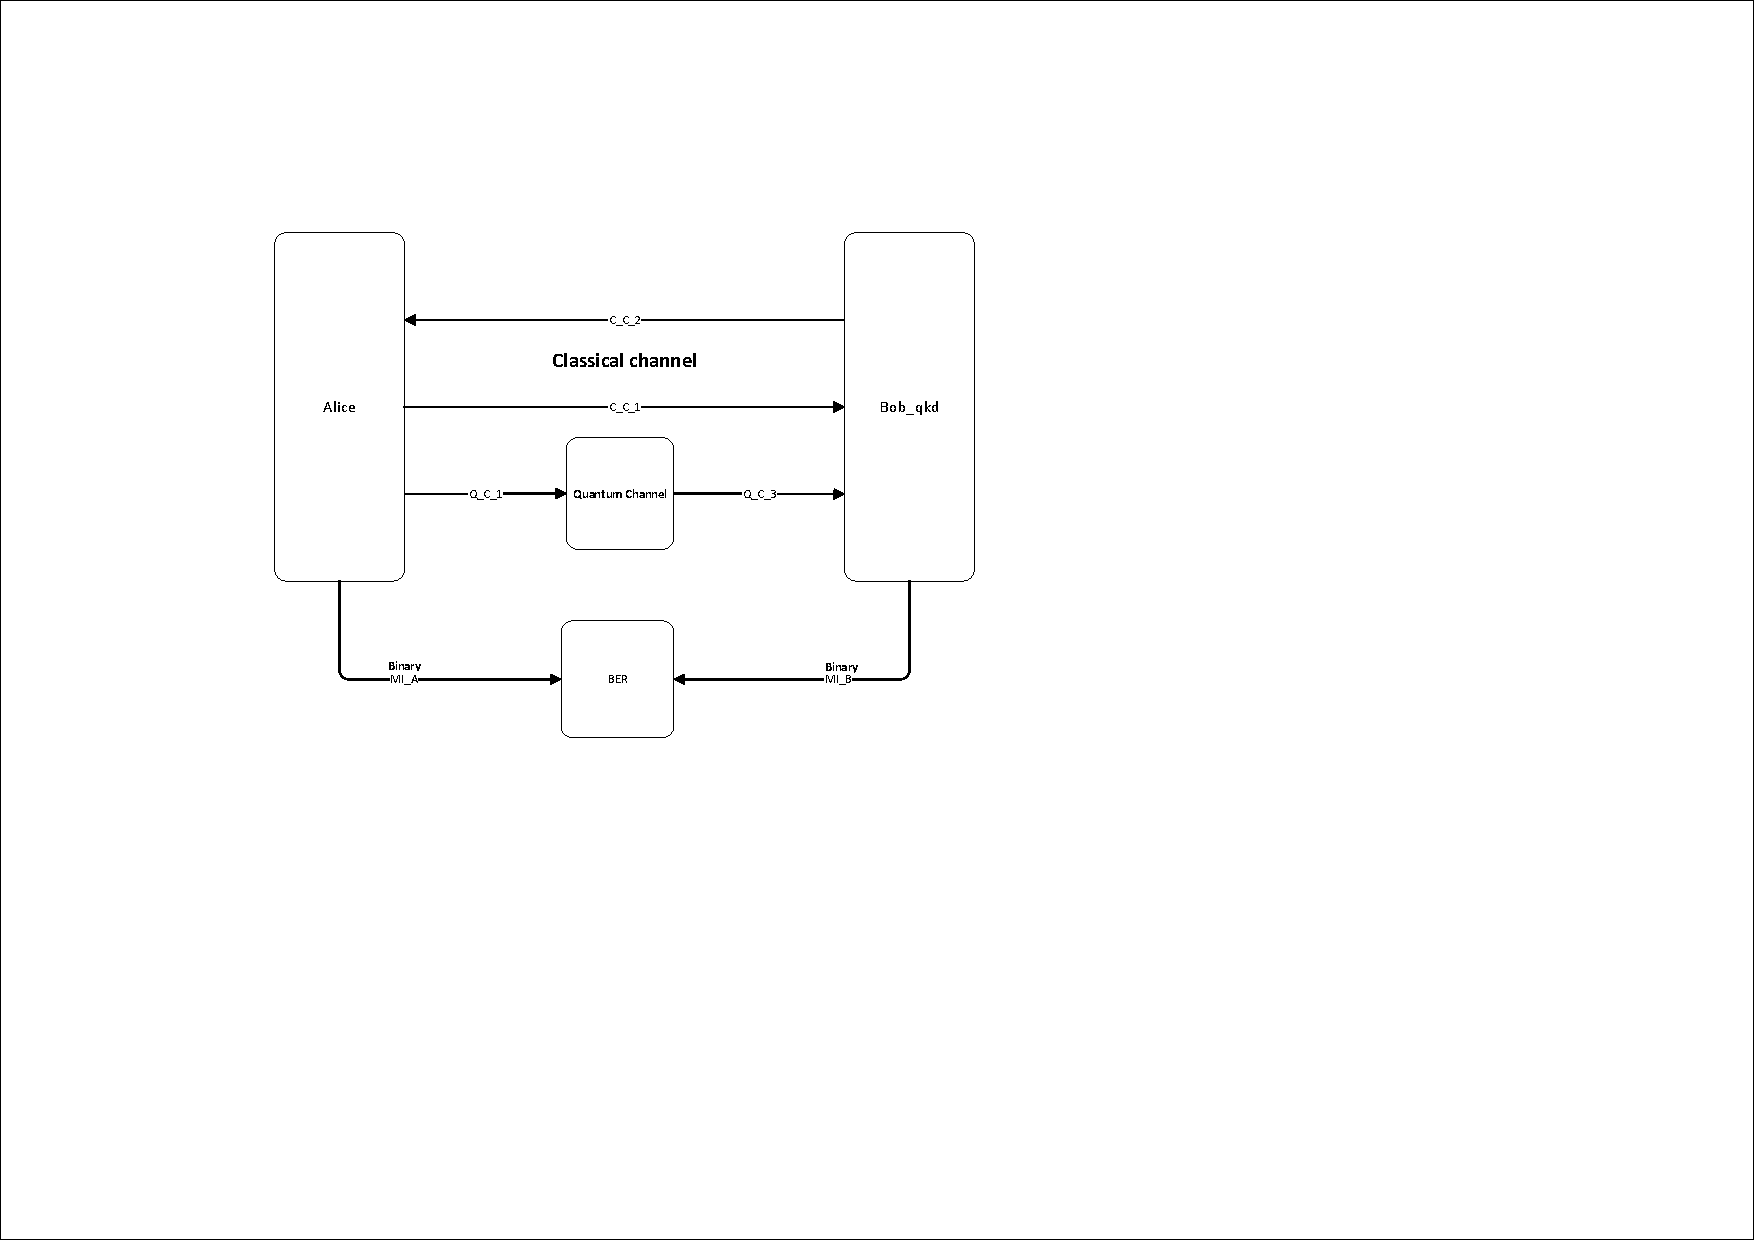
\includegraphics[clip, trim=1cm 8cm 10cm 3cm, width=1.00\textwidth]{./sdf/bb84_with_discrete_variables/figures/Simulation_toplevel_implemented.pdf}
    \caption{Simulation diagram at Alice's side}\label{simulationimplemented}
\end{figure}


Figure \ref{simulationimplemented} presents the top level diagram of our simulation. The setup contains two parties Alice and Bob, where the communication between them is done throughout two authenticated classical channels and one public quantum channel. In a first approach we will perform the simulation without eavesdropper presence. Furthermore, for bit error rate calculation between Alice and Bob.

\begin{figure}[h]
    \centering
        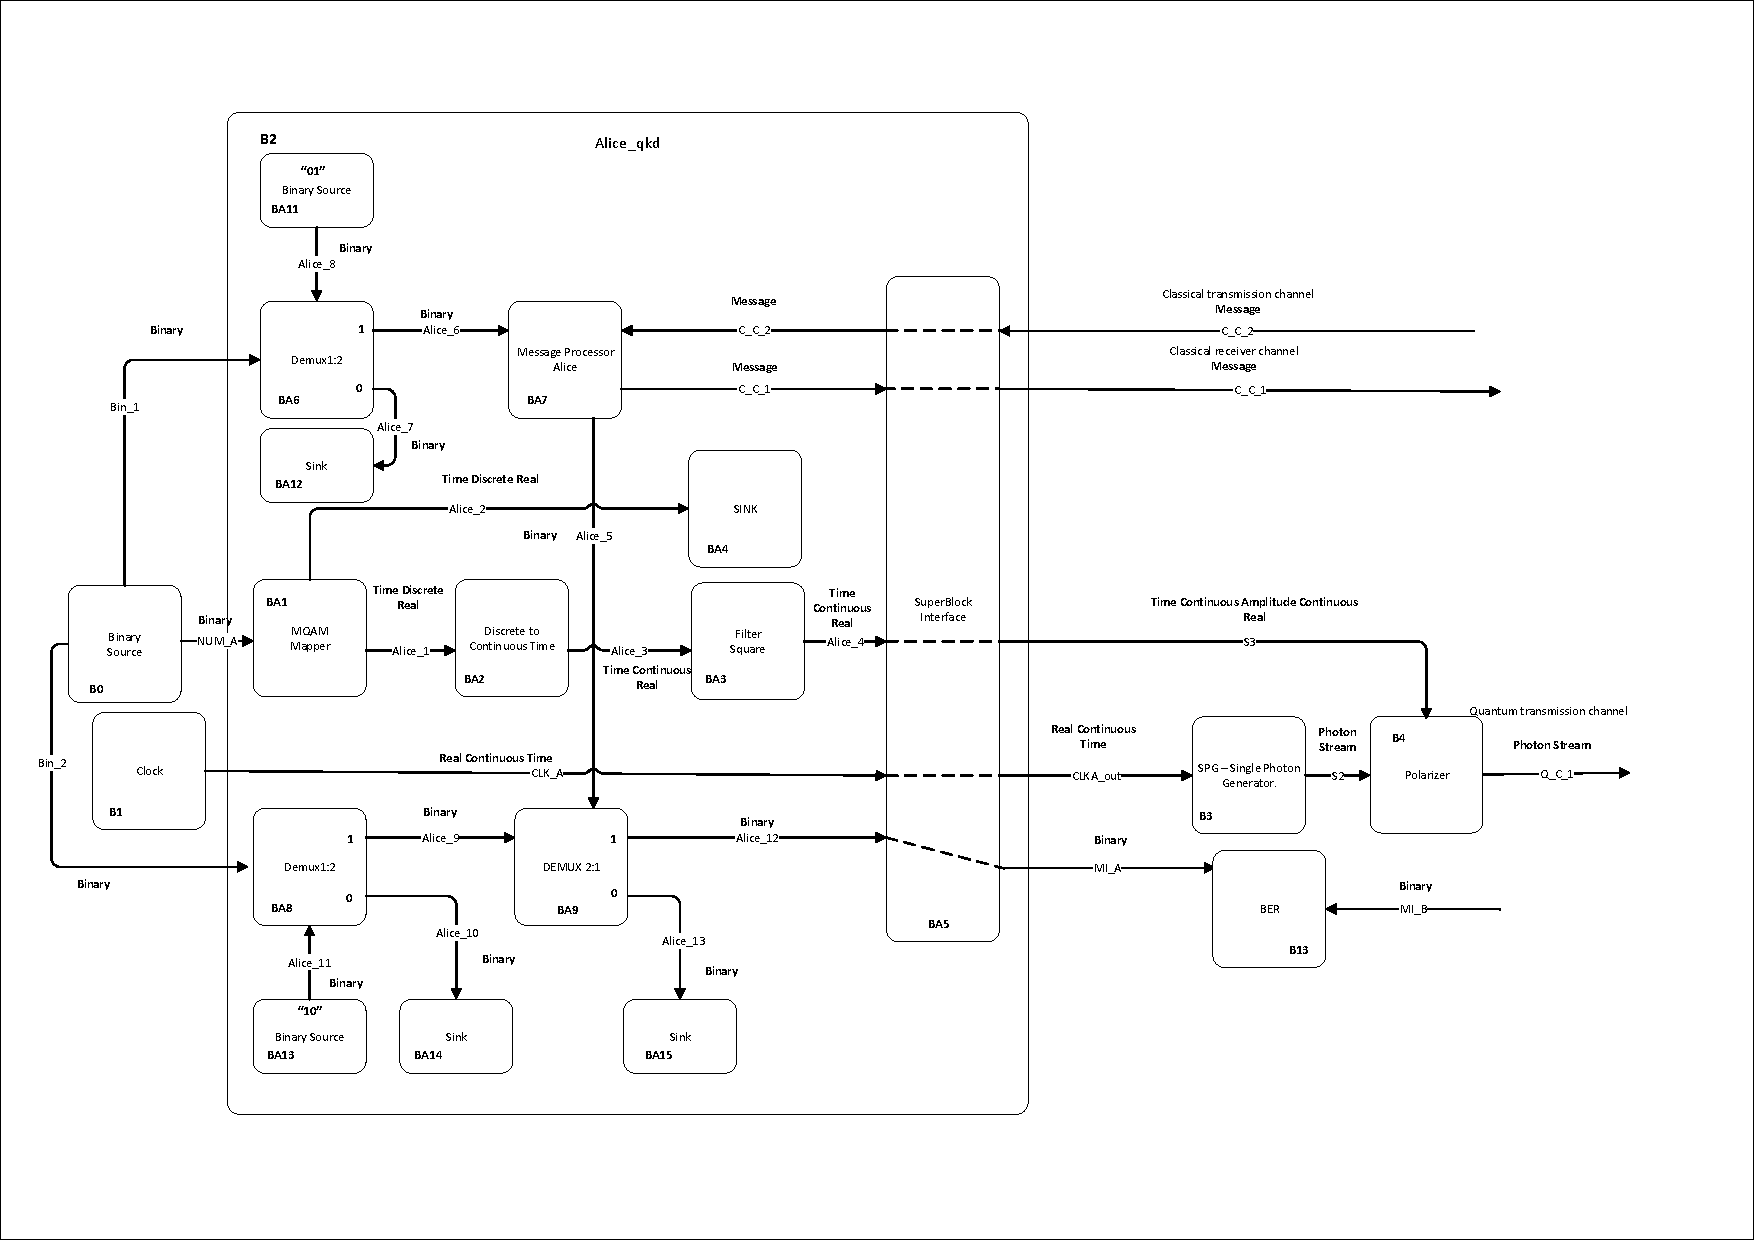
\includegraphics[clip, trim=0.5cm 1cm 0.5cm 1cm, width=1.10\textwidth]{./sdf/bb84_with_discrete_variables/figures/Simulation_Alice_bb84.pdf}
    \caption{Simulation diagram at Alice's side}\label{alicesimulation}
\end{figure}


\begin{figure}[h]
    \centering
        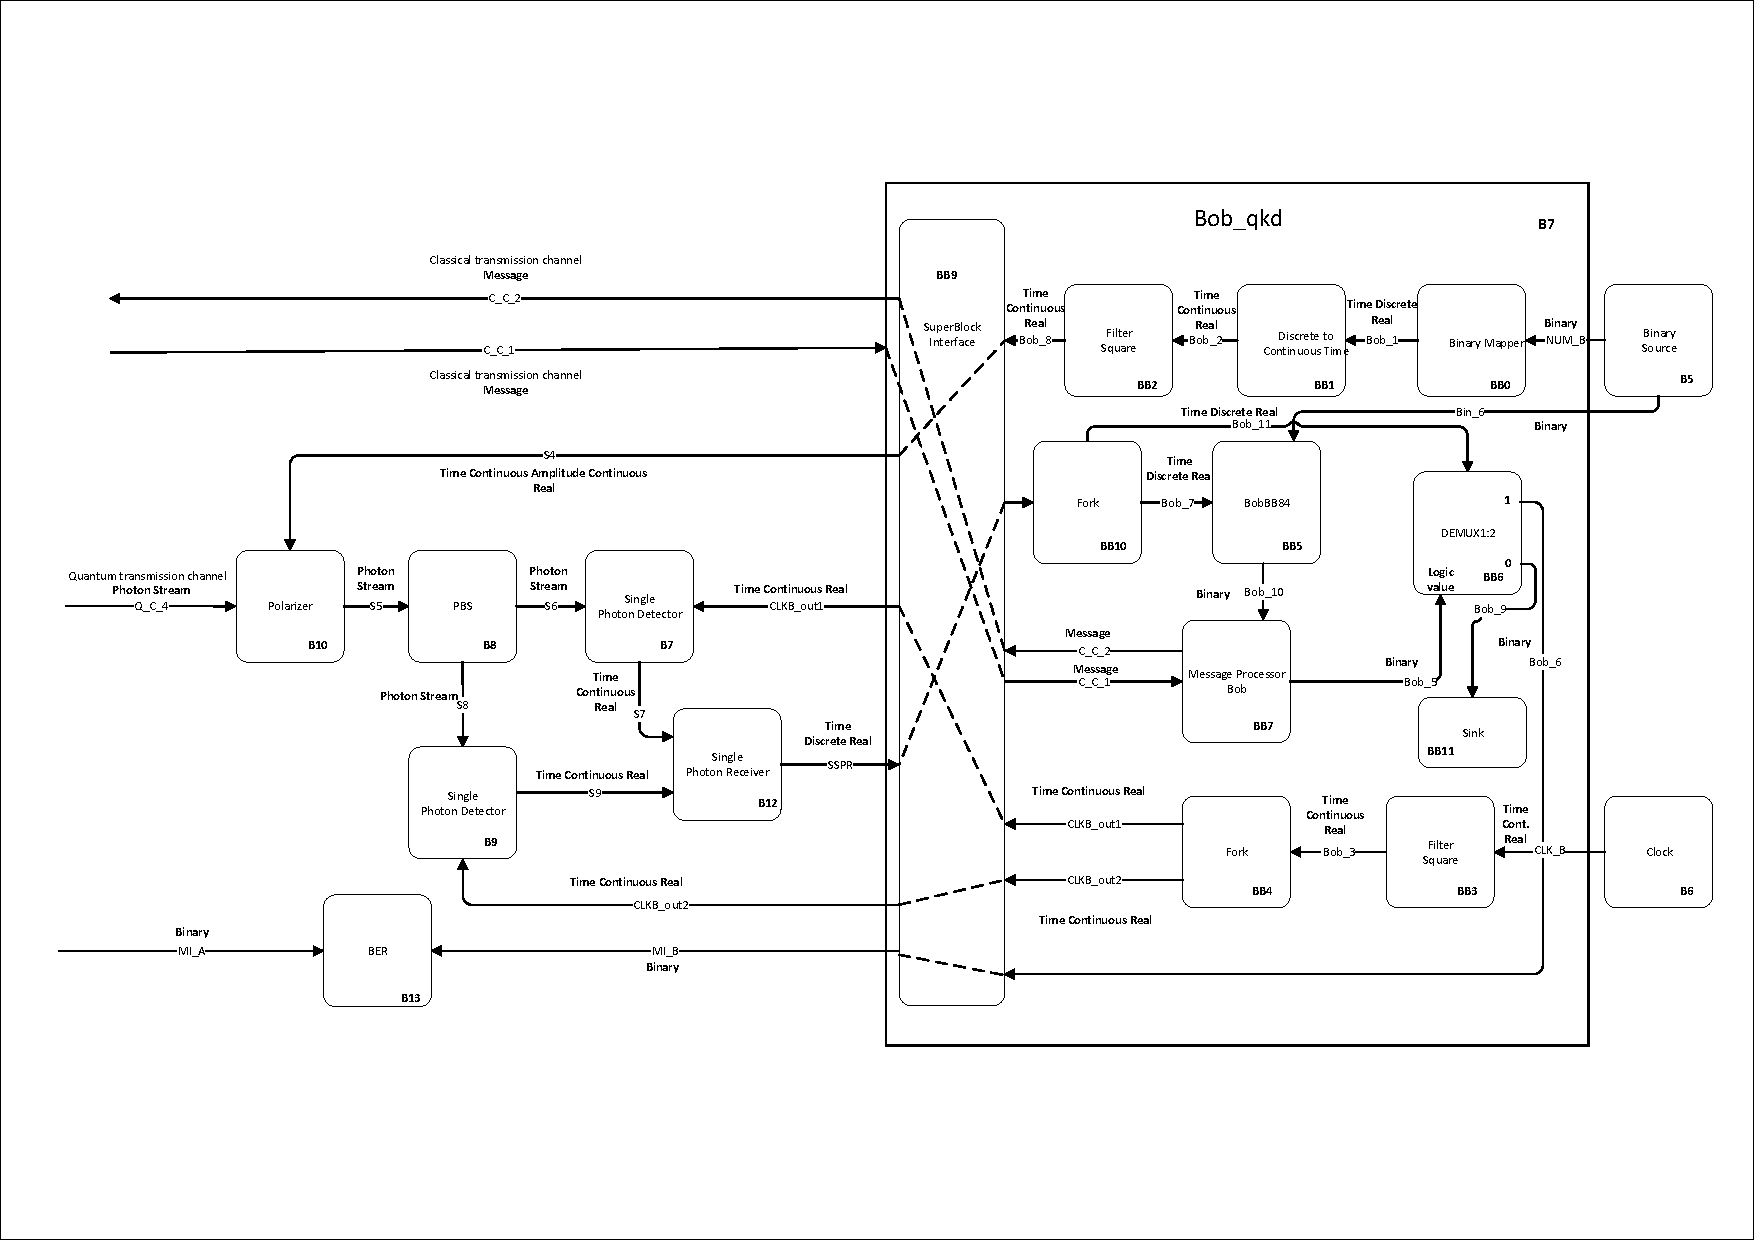
\includegraphics[clip, trim=0.5cm 2.0cm 0.5cm 0.5cm, width=1.00\textwidth]{./sdf/bb84_with_discrete_variables/figures/Simulation_Bob_bb84.pdf}
    \caption{Simulation diagram at Bob's side}\label{bobsimulation}
\end{figure}

    In figure \ref{alicesimulation} one can observe a block diagram of the simulation at Alice's side. As it is shown in the figure, Alice must have one block for random number generation which is responsible for basis generation to polarize the photons, and for key random generation in order to have a random state to encode each photon. Furthermore, she has a Processor block for all logical operations: array analysis, random number generation requests, and others. This block also receives the information from Bob after it has passed through a fork's block. In addition, it is responsible for set the initial length $l$ of the first array of photons which will send to Bob. This block also must be responsible for send classical information to Bob. Finally, Processor block will also send a real continuous time signal to single photon generator, in order to generate photons according to this signal, and finally this block also sends to the polarizer a real discrete signal in order to inform the polarizer which basis it should use. Therefore, she has two more blocks for quantum tasks: the single photon generator and the polarizer block which is responsible to encode the photons generated from the previous block and send them throughout a quantum channel from Alice to Bob.

    Finally, Alice's processor has an output to Mutual Information top level block, $Ms_{A}$.

    In figure \ref{alicesimulation} one can observe a block diagram of the transmitter. As it is shown in the figure, the transmitter must have one block for random number generation (binary source) which is responsible for basis generation to polarize the photons, and for key random generation in order to have a random state to encode each photon. This block has three outputs which will be inputs for the super block Alice. Furthermore, Alice block is responsible for all logical operations: random single photons state values generation, receive and send messages to the receiver Bob by using the classical channels, binary output for mutual information calculations. Each block of the super block is described in Library chapter. Finally, Alice block will also send a real continuous time signal to single photon generator (clock sets the rate oh photons generation), in order to generate photons polarized in the horizontal axis by default. Therefore, the transmitter has one more block, the polarizer block, which is responsible to encode the photons generated from the previous block and send them throughout a quantum channel from Alice to Bob.

     In figure \ref{bobsimulation} one can see a block diagram of the simulation for receiver (Bob). The receiver has one block for Random Number Generation which is responsible for randomly generate basis values which Bob will use to measure the photons sent by Alice throughout the quantum channel. Like transmitter, the receiver has the Bob block responsible for receive and send messages through the classical channel, receive single photons values detection from the single photon detectors, provides a clock signal to the detectors and send binary values for mutual information calculation. Furthermore, the receiver has two blocks for single photon detection (one for horizontal detection and other for vertical detection) which receives from Bob block a real continuous time signal which will set the detection window for the detector and outputs for Bob block the result value for detection. In addition, there is a polarizer which receives from Bob block a time continuous real signal which provides information about the rotation angle. If the basis chosen by Bob is the diagonal basis he sends "$45^\circ$", otherwise sends "$0^\circ$". The polarization beam splitter divides the input photon stream in horizontal component and vertical component.




%\begin{figure}[h]
%	\centering
%	\includegraphics[width=1.1\textwidth, height=14cm]{./sdf/bb84_with_discrete_variables/figures/eve_simulation.png}
%	\caption{Simulation diagram at Eve's side}\label{evesimulation}
%\end{figure}
%
%Figure \ref{evesimulation} presents the Eve's side diagram. Eve's processor has two receiver classical signals, one from Alice (\textbf{C\_C\_2}) and other from Bob (\textbf{C\_C\_5}). About quantum channel, Eve received a quantum message from Alice through the channel \textbf{Q\_C\_1} and depends on her decision the photon can follows directly to Bob or the photon's state can be changed by her. In this case, the photon is received by a block similar to Bob's diagram \ref{bobsimulation} and this block sends a message to Eve's processor in order to reveal the measurement result. After that, Eve's processor sends a message to Alice's diagram similar to figure \ref{alicesimulation} and this block is responsible for encode the photon in a new state. Now, the changed photon is sent to Bob.
%
%In addition, Eve's diagram has one more output $Ms_{E}$ which is a message sent to the mutual information block as an input parameter.

\begin{table}[H]
\centering
\caption{System Signals}
\label{tb:signals}
\begin{tabular}{|c|c|c|}
\hline
\textbf{Signal name}                        & \textbf{Signal type}                      \\ \hline
NUM\_A, NUM\_B, Bin\_1, Bin\_2, Bin\_6      &  Binary                                   \\ \hline
MI\_A, MI\_B                                &  Binary                                   \\ \hline
CLK\_A, CLK\_B                              &  TimeContinuousAmplitudeContinuous        \\ \hline
CLK\_A\_out, CLKB\_out1, CLKB\_out2         &  TimeContinuousAmplitudeContinuous        \\ \hline
S2, S5, S6, S8                              &  PhotonStreamXY                           \\ \hline
S3, S7, S9                                  &  TimeContinuousAmplitudeDiscreteReal      \\ \hline
S4                                          &  TimeContinuousAmplitudeContinuousReal      \\ \hline
C\_C\_1, C\_C\_3                            &  Messages                                 \\ \hline
C\_C\_6, C\_C\_4                            &  Messages                                 \\ \hline
Q\_C\_1, Q\_C\_4                            &  PhotonStreamXY                           \\ \hline

\end{tabular}
\end{table}

Table \ref{tb:signals} presents the system signals as well as them type.

\begin{table}[H]
\centering
\caption{System Input Parameters}
\label{tb:inputparameters}
\begin{tabular}{|c|c|c|}
\hline
\textbf{Parameter}                      & \textbf{Default Value}                                & \textbf{Description} \\ \hline
RateOfPhotons                           & 1K                                                    &                 \\ \hline
iqAmplitudeValues                       & \{-45,0\},\{0,0\},\{45,0\},\{90,0\}   &                 \\ \hline
NumberOfSamplesPerSylbom                & 16                                                    &                   \\ \hline
DetectorWindowTimeOpen                  & 0.2                                                   & smaller than 1 ms \\ \hline
DetectorPulseDelay                      & 0.7                                                   & in units of ms \\ \hline
DetectorProbabilityDarkCount            & 0.0                                                   &    \\ \hline
RotationAngle                           & 0.0                                                   & \\ \hline
ElevationAngle                          & 0.0                                                   & \\ \hline

\end{tabular}
\end{table}

\begin{table}[H]
\centering
\caption{Header Files}
\label{tb:signals}
\begin{tabular}{|c|c|c|}
\hline
\textbf{File name}                                          & \textbf{Description} & \textbf{Status} \\ \hline
netxpto\_20180118.h                                         &                      &    \checkmark      \\ \hline
alice\_qkd\_20180409.h                                      &                      &    \checkmark      \\ \hline
binary\_source\_20180118.h                                  &                      &    \checkmark      \\ \hline
bob\_qkd\_20180409.h                                        &                      &    \checkmark      \\ \hline
clock\_20171219.h                                           &                      &    \checkmark      \\ \hline
discrete\_to\_continuous\_time\_20180118.h                  &                      &    \checkmark      \\ \hline
m\_qam\_mapper\_20180118.h                                  &                      &    \checkmark      \\ \hline
polarization\_beam\_splitter\_20180109.h                    &                      &    \checkmark      \\ \hline
polarization\_rotator\_20180113.h                           &                      &    \checkmark      \\ \hline
pulse\_shaper\_20180111.h                                   &                      &    \checkmark      \\ \hline
single\_photon\_detector\_20180206.h                        &                      &    \checkmark      \\ \hline
single\_photon\_receiver\_20180303.h                        &                      &    \checkmark      \\ \hline
SOP\_modulator\_20180319.h                                  &                      &    \checkmark      \\ \hline
coincidence\_detector\_20180206.h                           &                      &    \checkmark      \\ \hline
single\_photon\_source\_20171218.h                          &                      &    \checkmark      \\ \hline
sink\_20180118.h                                            &                      &    \checkmark      \\ \hline
super\_block\_interface\_20180118.h                         &                      &    \checkmark      \\ \hline
message\_processor\_alice\_20180205.h                       &                      &    \checkmark      \\ \hline
demux\_1\_2\_20180205.h                                     &                      &    \checkmark      \\ \hline
binary\_mapper\_20180205.h                                  &                      &    \checkmark      \\ \hline
bobBB84\_20180221.h                                         &                      &    \checkmark      \\ \hline
message\_processor\_bob\_20180221.h                         &                      &    \checkmark      \\ \hline
sampler\_20171119.h                                         &                      &    \checkmark      \\ \hline
optical\_attenuator\_20180304.h                             &                      &    \checkmark      \\ \hline
fork\_20180112.h                                            &                      &    \checkmark      \\ \hline
\end{tabular}
\end{table}

\begin{table}[H]
\centering
\caption{Source Files}
\label{tb:signals}
\begin{tabular}{|c|c|c|}
\hline
\textbf{File name}                                          & \textbf{Description} & \textbf{Status}    \\ \hline
netxpto\_20180118.cpp                                       &                      &    \checkmark      \\ \hline
bb84\_with\_discrete\_variables\_sdf.cpp                    &                      &    \checkmark      \\ \hline
alice\_qkd\_20180409.cpp                                    &                      &    \checkmark      \\ \hline
binary\_source\_20180118.cpp                                &                      &    \checkmark      \\ \hline
bob\_qkd\_20180409.cpp                                      &                      &    \checkmark      \\ \hline
clock\_20171219.cpp                                         &                      &    \checkmark      \\ \hline
discrete\_to\_continuous\_time\_20180118.cpp                &                      &    \checkmark      \\ \hline
m\_qam\_mapper\_20180118.cpp                                &                      &    \checkmark      \\ \hline
polarization\_beam\_splitter\_20180109.cpp                  &                      &    \checkmark      \\ \hline
polarization\_rotator\_20180113.cpp                         &                      &    \checkmark      \\ \hline
pulse\_shaper\_20180111.cpp                                 &                      &    \checkmark      \\ \hline
single\_photon\_detector\_20180206.cpp                      &                      &    \checkmark      \\ \hline
single\_photon\_receiver\_20180303.cpp                      &                      &    \checkmark      \\ \hline
SOP\_modulator\_20180319.cpp                                &                      &    \checkmark      \\ \hline
coincidence\_detector\_20180206.cpp                         &                      &    \checkmark      \\ \hline
single\_photon\_source\_20171218.cpp                        &                      &    \checkmark      \\ \hline
sink\_20180118.cpp                                          &                      &    \checkmark      \\ \hline
super\_block\_interface\_20180118.cpp                       &                      &    \checkmark      \\ \hline
message\_processor\_alice\_20180205.cpp                     &                      &    \checkmark      \\ \hline
demux\_1\_2\_20180205.cpp                                   &                      &    \checkmark      \\ \hline
binary\_mapper\_20180205.cpp                                &                      &    \checkmark      \\ \hline
bobBB84\_20180221.cpp                                       &                      &    \checkmark      \\ \hline
message\_processor\_bob\_20180221.cpp                       &                      &    \checkmark      \\ \hline
sampler\_20171119.cpp                                       &                      &    \checkmark      \\ \hline
optical\_attenuator\_20180304.cpp                           &                      &    \checkmark      \\ \hline
fork\_20180112.cpp                                          &                      &    \checkmark      \\ \hline
\end{tabular}
\end{table}

\subsubsection{Simulation Results}

Figure \ref{toplevelalicebob} represents the block diagram of the first simulation performed between Alice and Bob. This simulation intends to simulate the communication protocol between Alice and Bob until they do the Basis Reconciliation. At this time, it is not taken into account any attack from an eavesdropper. However, as one can learn from theoretical protocol analysis, the attenuation due the fiber losses, dark counts probabilities from single photon detectors and the SOP drift over the quantum channel are all taken into account.

\begin{figure}[h]
    \centering
        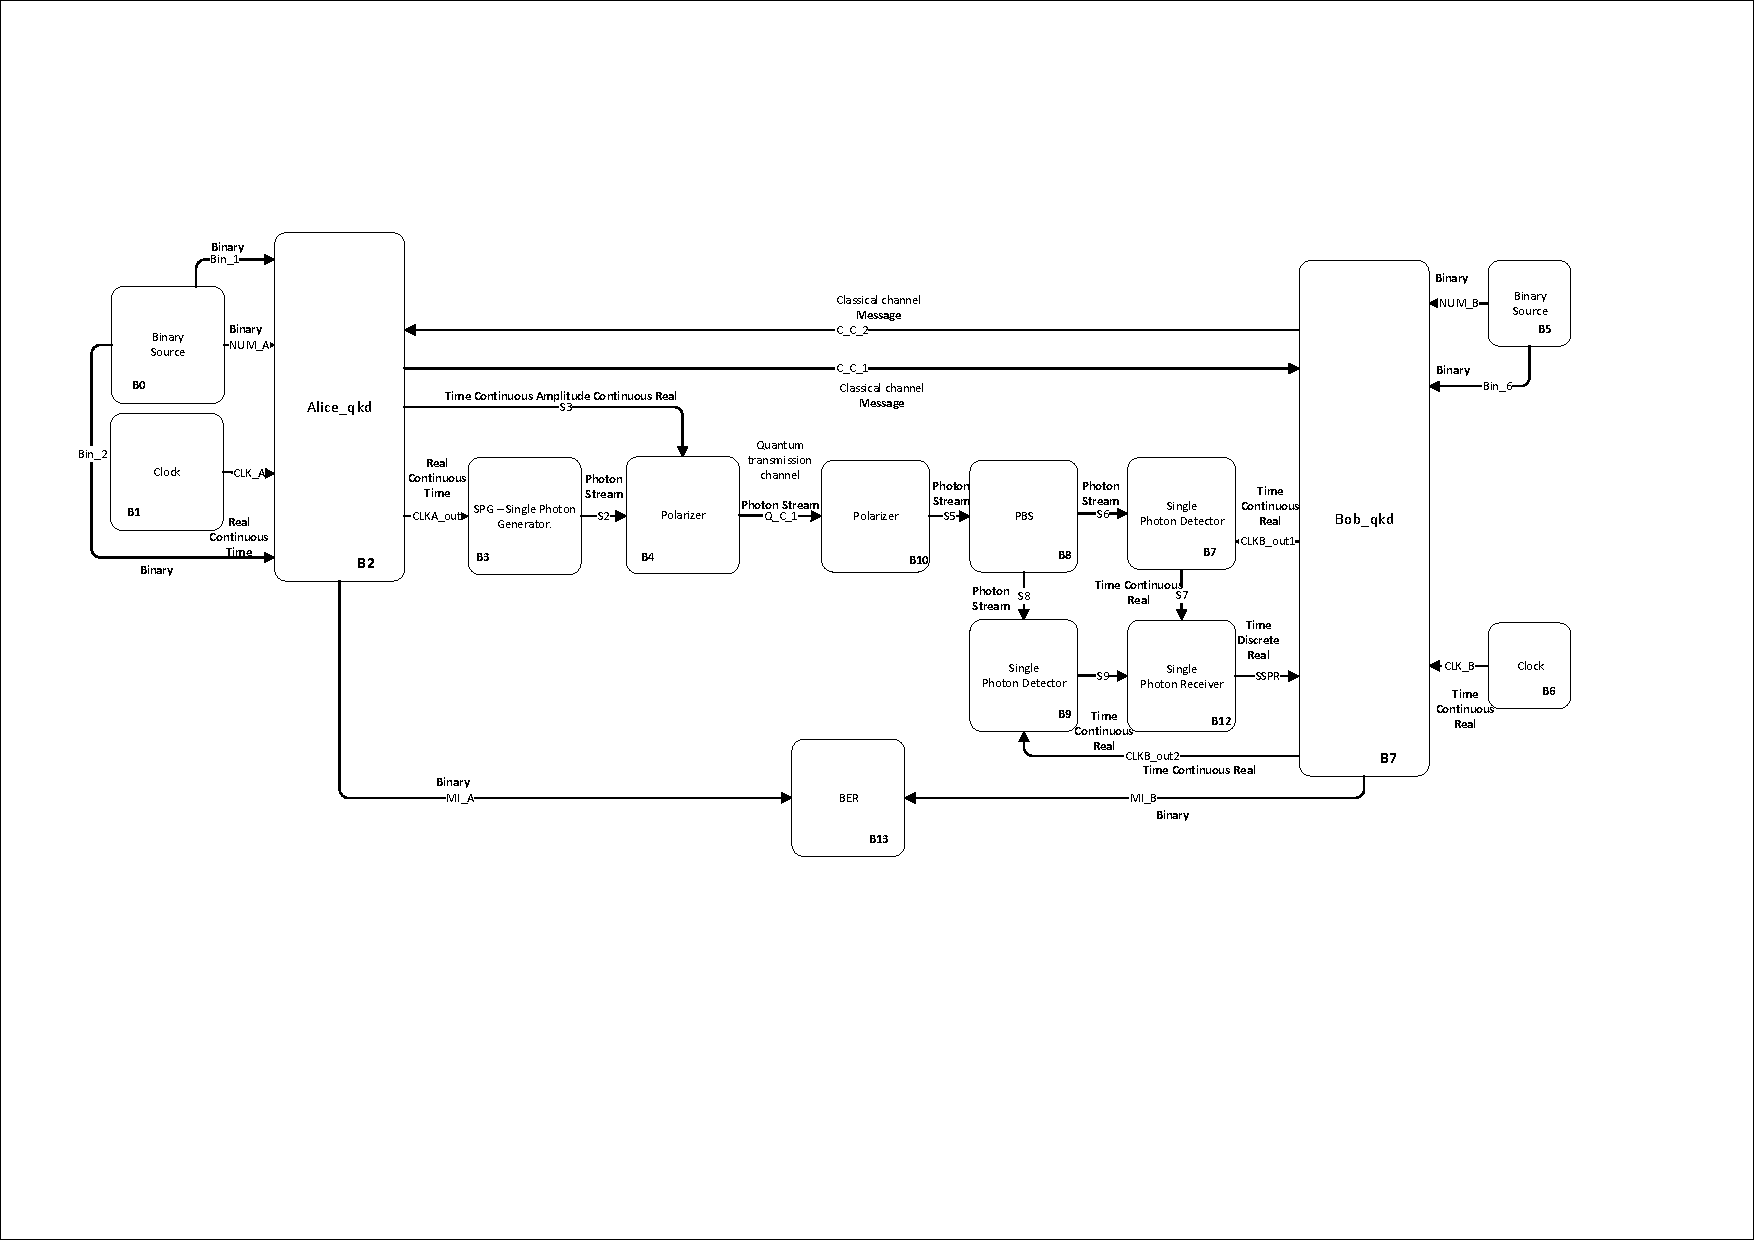
\includegraphics[clip=true, trim=1.2cm 5.0cm 0.5cm 2.5cm, width=1.10\textwidth]{./sdf/bb84_with_discrete_variables/figures/Simulation_toplevel_bb84.pdf}
    \caption{Diagram block of simulation performed between Alice and Bob until Basis Reconciliation. }\label{toplevelalicebob}
\end{figure}

Alice starts by sending a sequence of photons to Bob, and then he measures the photons according to random basis randomly generated by his binary source. After that, he follows the protocol described above until Alice sends to him a string of '0' and '1' where '0' means that both used different basis and '1' means that they used the same basis. Therefore, Alice and Bob outputs a binary signal "MI\_A" and "MI\_B", respectively. In case of no errors occurred in the quantum channel, these signals should be equal in order to both have the same sequence of bits. Furthermore, QBER between the two sequences should be $0$. This way, Alice can encode messages using these keys and Bob will be capable of decrypt the message using these symmetric keys. When errors are introduced in quantum channel QBER value will increase as we can see later.

\begin{figure}[H]
    \centering
        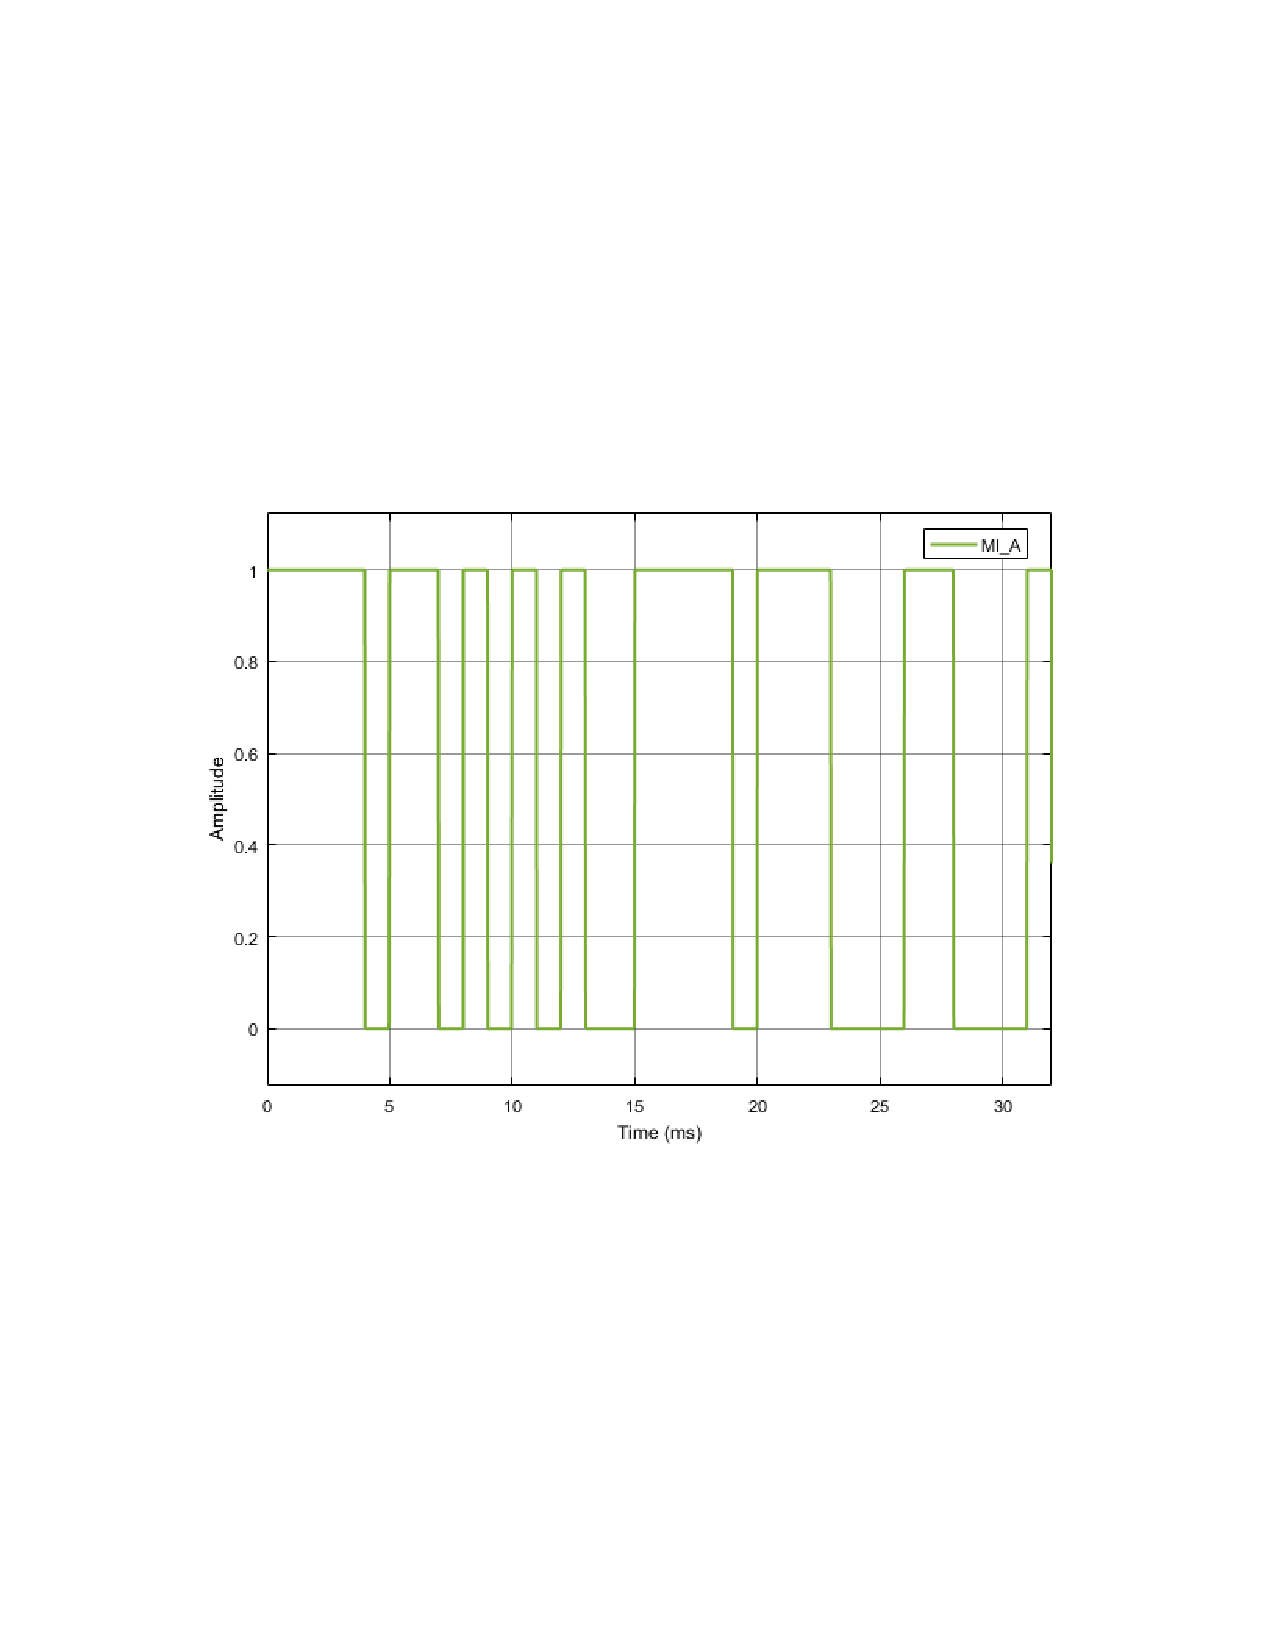
\includegraphics[clip, trim=3cm 9.0cm 2cm 7cm, width=0.50\textwidth]{./sdf/bb84_with_discrete_variables/figures/mia.pdf}
    \caption{MI\_A signal. }\label{mia}
\end{figure}

Figure \ref{mia} and figure \ref{mib} represent the sequence of bits which will be used by Alice to encode the messages and the sequence of bits used by Bob to decode the message when no errors in quantum channel are taken into account, respectively. As one can see the two signals are equal which meets the expected result. In this way, the first step of the protocol has been achieved.

\begin{figure}[h]
    \centering
        \includegraphics[clip, trim=3cm 9.5cm 2cm 7cm, width=0.50\textwidth]{./sdf/bb84_with_discrete_variables/figures/mib.pdf}
    \caption{MI\_B signal. }\label{mib}
\end{figure}

As one can see in figure \ref{toplevelsimulation} a block which calculates QBER is connected to Alice and Bob. This block calculates the QBER between the measurements that Bob performed with the same basis as Alice, based on method described in \cite{Muga11}. Thus, as expected, the QBER is $0 \%$ when no errors are taken into account.

Next, some errors due the changes in state of polarization of the single photons transmitted between Alice and Bob were added. This way, a polarization rotator in the middle of the quantum channel was added, which is controlled by a SOP modulator block as it is shown in figure \ref{sop_channel} with modelled with deterministic \cite{Muga15} and stochastic \cite{Czegledi16} methods. Additional information about the blocks presented in this quantum channel can be found in library chapter.

\begin{figure}[h]
    \centering
        \includegraphics[clip, trim=9cm 7.0cm 5cm 7.5cm, width=0.80\textwidth]{./sdf/bb84_with_discrete_variables/figures/Simulation_sop.pdf}
    \caption{Quantum channel diagram. }\label{sop_channel}
\end{figure}

Now, it is important to calculate the QBER as a function of the rotation angle $\theta$. In order to do that, it was simulated a deterministic SOP modulation, in which the $\theta$ angle varies over the time. In figure \ref{qber} is presented the variation in the value of QBER with respect with theta changes from $0^\circ$ to $45^\circ$. Theoretically, QBER corresponds to the probability of errors in the channel. Which means that in practice this probability corresponds to the probability of a photon following the wrong path in the polarization beam splitter immediately before the detection circuit.

\begin{figure}[h]
    \centering
        \includegraphics[clip, trim=4cm 17.0cm 5cm 5cm, width=0.80\textwidth]{./sdf/bb84_with_discrete_variables/figures/prob_qber.pdf}
    \caption{Representation of two orthogonal states rotated by an angle $\theta$.}\label{rep_rotation}
\end{figure}

Figure \ref{rep_rotation} presents the graphical representation of two orthogonal states rotated by an angle $\theta$. This rotation is induced by the SOP modulator block which selects a deterministic $\theta$ and $\phi$ angles that do not change over the time. This same rotation is applied for all sequential samples. From figure \ref{rep_rotation} the theoretical QBER can be calculated using the following equation:

\begin{equation}\label{eq:qber}
  QBER = P(0)P(1|0)+P(1)P(0|1).
\end{equation}

Since we have been using a polarization beam splitter 50:50,

\begin{equation*}
  P(0) = P(1) = \frac{1}{2}.
\end{equation*}

This way,
\begin{eqnarray}\label{eq:qber_final}
% \nonumber % Remove numbering (before each equation)
   QBER & = & \frac{1}{2}sin^2(\theta)+ \frac{1}{2}sin^2(\theta)\\
   QBER & = & sin^2(\theta).
\end{eqnarray}

 In figure \ref{qber} are represented two curves: QBER calculated from simulated data and QBER calculated using theoretical model from equation \ref{eq:qber_final}. Furthermore, the cross correlation coefficient between the two signals was calculated using a function from MATLAB \textit{xcorr(x,y,'coeff')} which the result is $99.92\%$. From that, we can conclude that the QBER calculated from simulated data follows the theoretical curve with high correlation. Nevertheless, the error bars presented in figure \ref{qber} were calculated based on a confidence interval of $95\%$.

\begin{figure}[h]
    \centering
        \includegraphics[clip, trim=0.5cm 0.0cm 0.5cm 1cm, width=0.80\textwidth]{./sdf/bb84_with_discrete_variables/figures/QBER_vs_theta_normal_scale.pdf}
    \caption{QBER evolution in relation with deterministic SOP drift.}\label{qber}
\end{figure}

\begin{figure}[H]
    \centering
        \includegraphics[clip, trim=0.2cm 0.0cm 0.5cm 1cm, width=0.80\textwidth]{./sdf/bb84_with_discrete_variables/figures/qber_vs_theta_all.pdf}
    \caption{QBER evolution in relation with deterministic SOP drift in log scale.}\label{qber_log}
\end{figure}

\begin{figure}[H]
    \centering
        \includegraphics[clip, trim=0.2cm 0.0cm 0.5cm 1cm, width=0.80\textwidth]{./sdf/bb84_with_discrete_variables/figures/QBER_vs_theta_upto15.pdf}
    \caption{QBER evolution in relation with deterministic SOP drift scaled.}\label{qber_log_scaled}
\end{figure}
\newpage

\subsection{Open Issues}
\begin{enumerate}

    \item Implementation of the control system for polarization rotations.
    \item Implementation of a QBER estimation protocol.
    \item Implementation of the scrambling algorithm in order to spread the errors.
    \item Implementation of the cascade for error correction.
    \item Implementation of the output which represents the final key that is built.
    \item Introduce EVE in simulation as shown in figure \ref{toplevelsimulation2}.
        \begin{figure}[H]
        	\centering
        	\includegraphics[width=1.0\textwidth, height=9cm]{./sdf/bb84_with_discrete_variables/figures/toplevel_simulation.png}
        	\caption{Simulation diagram at a top level}\label{toplevelsimulation2}
        \end{figure}
    \item Analyze different strategies for Eve.  
    \item Experimental Implementation.
\end{enumerate}



\newpage


% COLOCAR ESTAS REFERÊNCIAS NUM FICHEIRO BIB
%
%\begin{thebibliography}{2}
%	\bibitem{BB84}
%	Bennett, C. H. and Brassard,
%	G. Quantum Cryptography: Public key distribution and coin tossing.
%	International Conference on Computers, Systems and Signal Processing, Bangalore, India, 10-12 December 1984, pp. 175-179.
%	
%	\bibitem{SURV}
%	Mart Haitjema, A Survey of the Prominent Quantum Key Distribution Protocols
%	
%	\bibitem{iqo}
%	Christopher Gerry, Peter Knight, "Introductory Quantum Optics" Cambridge University Press, 2005
%	
%	\bibitem{SPREADING}
%	Varadarajan, S., Ngo, H. Q., \& Srivastava, J. (n.d.). An Adaptive , Perception-Driven Error Spreading Scheme in Continuous Media Streaming.
%	
%\end{thebibliography}

% bibliographic references for the section ----------------------------
\clearpage
\printbibliography[heading=subbibliography]
\end{refsection}
\addcontentsline{toc}{subsection}{Bibliography}
\cleardoublepage
% ---------------------------------------------------------------------  \fi
\ifdefined\qokd         \clearpage
\section{Quantum Oblivious Key Distribution with Discrete Variables}

\begin{tcolorbox}	
\begin{tabular}{p{2.75cm} p{0.2cm} p{10.5cm}} 	
\textbf{Student Name}  &:& Mariana Ramos\\
\textbf{Starting Date} &:& September 18, 2017\\
\textbf{Goal}          &:& Quantum oblivious key distribution (QOKD) implementation with discrete variables.\\
\textbf{Directory}     &:& sdf/ot\_with\_discrete\_variables.
\end{tabular}
\end{tcolorbox}

Oblivious Transfer (OT) is a fundamental primitive in multi-party computation. The one-out-of-two OT consists in a communication protocol between Alice and Bob. At the beginning of the protocol Alice has two messages $m_1$ and $m_2$ and Bob wants to know one of them, $m_b$, without Alice knowing which one, i.e. without Alice knowing $b$, and Alice wants to keep the other message private, i.e. without Bob knowing $m_{\bar{b}}$. therefore two conditions must be fulfilled:
\begin{enumerate}
	\item{The protocol must be concealing, i.e at the beginning of the protocol Bob does not know nothing about Alice's messages, while at the end of the protocol Bob will learn the message $m_{b}$ chosen by him.}
	\item{The protocol is oblivious, i.e Alice cannot learn anything about Bob's choice, bit $b$, and Bob cannot learning nothing about the other message $m_{\bar{b}}$.}
\end {enumerate}

In order to implement OT between two parties (Alice and Bob) they must be able to exchange continuously oblivious keys, i.e a QOKD system must exist between them.

\subsection{Quantum Oblivious Key Distribution System (QOKD)}

In this section we are going to describe the Quantum Oblivious Key Distribution system (QOKD).
The QOKD system enables two parties (Alice and Bob) to share a set of keys. These keys have the particularity of being half right and half wrong. Only Bob knows which are right and wrong keys.

Considering a discrete variables implementation, both Alice and Bob agree with the following correspondence, where $+$ corresponds to \textit{Rectilinear Basis} and $\times$ corresponds to \textit{Diagonal Basis},

\begin{table}[H]
\centering
\begin{tabular}{c|c}
\textbf{\textit{Basis}}         &  \\ \hline
 0 & $+$ \\
 1 & $\times$ \\
\end{tabular}
\end{table}
Alice and Bob also agree with the bit correspondence for each direction for each basis. For \textit{Rectilinear basis}, "$+$",

\begin{table}[H]
\centering
\begin{tabular}{c|c}
            & Basis "+" \\ \hline
 0 & $\to (0^{\circ})$ \\
 1 & $\uparrow (90^{\circ})$ \\
\end{tabular}
\end{table}
and for \textit{Diagonal Basis}, "$\times$",

\begin{table}[H]
\centering
\begin{tabular}{c|c}
      & Basis "$\times$" \\ \hline
 0 & $\searrow (-45^{\circ})$ \\
 1 & $\nearrow (45^{\circ})$ \\
\end{tabular}
\end{table}

\begin{enumerate}
  \item The first step is to establish for both Alice and Bob the block length $l$. In this case, lets assume $l=16$. Alice randomly generate a bit sequence with length $l$.
      Therefore, she must define two sets randomly: $S_{A1}$ which contains the basis values; and $S_{A2}$, which contains the key values.

      In that case, lets assume she generates the following sets $S_{A1'}$ and $S_{A2'}$:
      $$S_{A1'} = \{0,0,1,1,1,0,0,1,1,0,0,1,1,1,0,1 \},$$
      $$S_{A2'} = \{1,1,1,0,0,0,0,0,1,1,0,0,1,0,1,1 \}.$$

  \item Next, Alice sends to Bob throughout a quantum channel $l$ photons encoded using the basis defined in $S_{A1'}$ and according to the key bits defined in $S_{A2'}$.

      Therefore, in the current example, Alice sends the following photons,

      \begin{align*}
        S_{AB} & = \{\space { }\uparrow \ \space { }\space { },\space { }\uparrow \ \space { }\space { }, \space { }\nearrow \ \space { }\space { },\space { } \searrow \ \space { }\space { } \ , \space { }\searrow \ \space { }\space { }, \to \ , \to \ ,\space { } \searrow \ \space { }\space { },\space { } \nearrow \ \space { },\space { }\uparrow \ \space { }\space { }, \space { }\to \ ,\space { } \searrow\space { }\space { },\space { }\nearrow\space { }\space { },\space { }\searrow \ \ \space { }\space { },\space { }\uparrow \ \space { }\space { },\space { }\nearrow \space { }\space { }\} \\
          & =\{90^{\circ},90^{\circ}, 45^{\circ}, -45^{\circ},-45^{\circ}, 0^{\circ}, 0^{\circ}, -45^{\circ}, 45^{\circ},90^{\circ}, 0^{\circ}, -45^{\circ}, 45^{\circ}, -45^{\circ}, 90^{\circ}, 45^{\circ} \}.
        \label{eq:photonsalice}
      \end{align*}


  \item Bob also randomly generates $l=16$ bits, which are going to define his measurement basis, $S_{B1'}$. Lets assume,
        \begin{align*}
             S_{B1'} & = \{0 \ ,1 \ ,1 \ ,0 \ ,0 \ ,1 \ ,0 \ ,1 \ ,1 \ ,0 \ ,1 \ ,1 \ ,0 \ ,0 \ ,0 \ ,1 \  \} \\
                    & = \{ +,\times,\times,+,+,\times,+,\times, \times,+, \times, \times \,+,+,+,\times \}.
        \end{align*}

      Bob will get $l$ results:
      $$S_{B2'} = \{1,-,\underline{0},0,-,1,\underline{1},-,1,-,1,0,1,1,\underline{0},1 \}.$$

      The "$-$"\space{ } corresponds to no clicks in Bob's detector, due to attenuation. The underlined values are bits which were measured with a correct basis but an error has occurred due to imperfections in the quantum communication system.

  \item Bob is going to send a "$-1$"\space{ } or a hash value to Alice for each measurement that he performed, thereby being "$-1$"\space{ } the measurements which correspond to no clicks. In this case, we are going to assume that the hash value is calculated using the \textit{SHA-256} algorithm \cite{Liu2009}. In detail, Bob has two sets $S_{B1'}$ and $S_{B2'}$ and he is going to generate the set $S_{BH1}$ with $l$ values ("$-1$"\space{ } or hash values calculated for each position of $S_{B1'}$ with the correspondent position of $S_{B2'}$). Therefore, Bob will send to Alice the following set:
      $$S_{BH1}=\{{S}_{1},-1,{S}_{2},{S}_{3}, -1,{S}_{4},{S}_{5},-1,{S}_{6},-1,{S}_{7},{S}_{8},{S}_{9},{S}_{10},{S}_{11},{S}_{12} \}.$$


  \item Since Alice has received the confirmation of measurement from Bob, i.e after Alice has received $S_{BH1}$, she sends throughout a classical channel the basis which she has used to codify the photons updated with the information about the no received photons, $$S_{A1'} = \{0,-1,1,1,-1,0,0,-1,1,-1,0,1,1,1,0,1 \}$$.

      Due to attenuation, the previous sets are reduced to the length $12$ and they shall be replaced by the following:
      $$S_{A1}=\{0,1,1,0,0,1,0,1,1,1,0,1 \},$$
      $$S_{A2}=\{1,1,0,0,0,1,0,0,1,0,1,1 \},$$
      $$S_{B1}=\{0,1,0,1,0,1,1,1,0,0,0,1 \},$$
      $$S_{B2}=\{1,\underline{0},0,1,\underline{1},1,1,0,1,1,\underline{0},1 \}$$
      Note that $S_{B2}$ still has errors.

  \item In order to know which photons were measured correctly, Bob does the operation $S_{B3}=S_{B1} \oplus S_{A1}$.
      In the current example,

  \begin{table}[H]
    \centering
    \begin{tabular}{c|c c c c c c c c c c c c }
     $S_{B1}$ & 0 & 1 & 0 & 1 & 0 & 1 & 1 & 1 & 0 & 0 & 0 & 1\\
     $S_{A1}$ & 0 & 1 & 1 & 0 & 0 & 1 & 0 & 1 & 1 & 1 & 0 & 1\\ \hline
     $\oplus$ & 1 & 1 & 0 & 0 & 1 & 1 & 0 & 1 & 0 & 0 & 1 & 1
    \end{tabular}
    \end{table}

      In this way, Bob gets $$S_{B3} = \{1,1,0,0,1,1,0,1,0,0,1,1 \}.$$ When Bob uses the right basis he gets the values correctly, apart from possible errors in transmission, when he uses the wrong basis he just guess the value. The values "1"\space{ } correspond to the values he measured correctly and "0" \space{ }to the values he just guessed.
      Thus, Bob is building two sets of keys, one with correct basis measurements values and other with the wrong basis measurement values that he just guessed.

      Thus, Bob has two pair of sets, one for the right basis,

      $$S_{B_{rp}}= \{1,2,5,6,8,11,12 \},$$ $$ S_{B_{rb}} = \{1,0,1,1,0,0,1 \},$$
      where $S_{B_{rp}}$ is the set of positions and $SB_{rb}$ is the set of bit values he measured for each position. The other pair is for photons he measured with the wrong basis and then he just guessed the values,
      $$S_{B_{wp}}= \{3,4,7,9,10 \},$$ $$S_{B_{wb}} = \{0,1,1,1,1 \},$$
      where $S_{B_{wp}}$ is the set of positions and $S_{B_{wb}}$ is the set of bit values he measured for each position.

      Nevertheless, due to errors in transmission, some bits in $S_{B_{rb}}$ may be not right.

      At this point, in order to test Bob's honesty and to estimate the \textit{QBER} of the channel, Alice is going to ask Bob to open some pairs of the Bob's sets. The definition of the protocol to test Bob's honesty is still an open issue. However, depending on the \textit{QBER} estimated by her, Alice must have a parameter to set the number of right position she wants to open, i.e she must open a minimum number of right position in order to guarantee a minimum \textit{QBER}. This will increase the security of the protocol. Alice chooses some positions to open and tells Bob which positions she wants to open. Bob sends to Alice the pairs she chose and then these pairs are eliminated from them sets. Lets assume she asked to open the positions $10$, $11$ and $12$. If she concludes Bob is not being honest, she stops the protocol and they must start it again. Otherwise, the protocol continues. Lets assume Alice has verified these pairs using the hash function committed by Bob and concluded that he is being honest. Therefore, she sends to Bob the \textit{QBER} estimated by her.

      Now, Bob has the previous sets replaced by the following,
      \begin{align*}
        S_{B_{rp}} & = \{1,2,5,6,8 \} \\
        S_{B_{rb}} & = \{1,0,1,1,0 \} \\
        S_{B_{wp}} & = \{3,4,7,9 \} \\
        S_{B_{wb}} & = \{0,1,1,1 \}
      \end{align*}


      Bob is going to use a modified version of \textit{Cascade algorithm} to correct the errors due transmission.

      \subsubsection{Modified version of Cascade Algorithm}
      The Cascade algorithm is often used with a key set where all values are supposed right. In this case, Bob has two pairs of sets, one with the position and bit values of photon he measured with the correct basis and other with position and bit values of photon he measured with the wrong basis. He only needs to apply the Cascade algorithm in the set that he measured the photons correctly \cite{Brassard1994}. However, he must apply a modified version of the Cascade in the other set in order to keep in secret from Alice which set corresponds to right and which set corresponds to wrong measurements.

      Bob randomly generates a bit value. If he gets $0$, he will send to Alice the set $\{ S_{B_{rp}}, S_{B_{wp}}\}$. Otherwise, if he gets $1$ he will send the set $\{S_{B_{wp}}, S_{B_{rp}}\}$. This guarantee that Alice does not know which is the right or wrong set. Lets assume this random bit is "0" and he sends $\{S_{B_{rp}}, S_{B_{wp}}\}$.

      \begin{enumerate}
        \item Bob starts by applying the normal cascade to the set $S_{B_{rb}}$. After both know the error estimative Bob determine if the error rate is above the fail threshold. If it is truth they must start the procedure again. Lets assume the estimated error rate is acceptable. Bob and Alice use a random permutation which is represented in figure \ref{cascadepermutation} for a larger number of bits (agreed at the beginning) by applying it to the shifted keys, in order to guarantee the spread out of the error bits randomly and to separate consecutive errors from each other.

            \begin{figure}[h]
            	\centering
            	\includegraphics[width=0.6\textwidth, height=4cm]{./sdf/qokd_with_discrete_variables/figures/cascade_permutation.png}
                	\caption{Cascade Algorithm - permutation}\label{cascadepermutation}
            \end{figure}

        \item Bob and Alice divide all the shifted key bits into blocks of N bits depending on the estimated error rate in order to have one or no error per block. In general, the sets of keys are too large and it is easier to explain the algorithm based on a larger number of bits. Therefore, figure \ref{cascade_1} represents the typical cascade initial steps. However, in this case, the set to be corrected only has five bits, therefore they divide the set in two sub-blocks, one with $3$ bits and other with $2$ bits.

             \begin{figure}[h]
            	\centering
            	\includegraphics[width=0.8\textwidth, height=6cm]{./sdf/qokd_with_discrete_variables/figures/cascade_1.png}
                	\caption{Cascade Algorithm}\label{cascade_1}
            \end{figure}

        \item They use a classical channel to compare the block parities. For blocks with different parities, an odd number of errors must exist, otherwise an even number of errors would mask each other. Thus, the block in which the parities disagree is divided in half into two smaller blocks of length $\frac{N}{2}$, and another parity check is performed on the first sub-block, as one can see in figure \ref{cascade_2}. As it was referred above, there is at least one error in one sub-block being the error location revealed by the parity of one sub-block. In other words, if the parity of the first sub-block passes, the error will be in the second sub-block. The sub-block with error will be sub-divided until the error is found.

            \begin{figure}[h]
            	\centering
            	\includegraphics[width=0.6\textwidth, height=6cm]{./sdf/qokd_with_discrete_variables/figures/cascade_2.png}
                	\caption{Cascade Algorithm - example of error correction}\label{cascade_2}
            \end{figure}

        \item When the error is corrected, the last bit of the block is discard in order to prevent the gain of additional information by Bob.


            In this case, lets assume the set of right positions was corrected with the algorithm described above and it will be replaced by the following:

            \begin{align*}
              S_{B_{rp}} & = \{1,2,5,6,8 \} \\
              S_{B_{rb}} & = \{1,1,0,1,0 \} \\
            \end{align*}

             In order to test Alice's honesty, Bob must verify if the \textit{QBER} sent by Alice is a realistic value. If it is not he stops the protocol and they must start again. Otherwise, the protocol continues.

      \end{enumerate}

      After that, Bob needs to apply the Fake Cascade to the set $S_{B_{wb}}$. The main goal of this step is to convince Alice she is performing the real Cascade but she is not.

      \begin{enumerate}
        \item First of all, based on the positions contained in $S_{B_{wb}}$, Bob must build an array with the correspondent bits in a random order and informs Alice the order of positions. In order to best explain this version of the algorithm, lets assume a larger set of bits.

            Bob sends to Alice throughout a classical channel the new positions order as if it were the permutation step represented in figure \ref{cascadepermutation} in real Cascade algorithm.

        \item Assuming each of them has a set with 32 bits randomly organized by Bob, they divide the supposed shifted keys in blocks with N bits according to the estimated error rate. As the \textit{QBER} is the same as for real cascade, Bob will assume the same number of errors, even if he starts for this modified version he can know the number of errors from \textit{QBER} estimated by Alice.

        \item Bob and Alice use a classical channel to compare the block parities. Alice sends to Bob her parity list. Based on Alice's parity list, Bob sends a block list with odd parities, i.e the blocks position in which parity supposed disagree. This list is randomly built based on the number of errors considered by Bob, i.e if he considered five errors from \textit{QBER} estimative, he will distributed them randomly and after that he will fill the remaining spaces with even parities. Bob sends to Alice the set with the list of odd parities, i.e the list of sub-sets he has different parities than Alice.

        \item The blocks with errors will be consecutively divided until they found the supposed errors. Since we have assumed there were five errors, this is the number of errors that Alice must supposedly correct.

            \begin{figure}[h]
            	\centering
            	\includegraphics[width=0.6\textwidth, height=6cm]{./sdf/qokd_with_discrete_variables/figures/fake_cascade.png}
                	\caption{Fake cascade - example of error correction}\label{fake cascade}
            \end{figure}

            Lets assume one of the blocks with error and analyse figure \ref{fake cascade}. Bob starts with a set filled with random bits, therefore we do not need to know which bits are. Alice starts by dividing her set in half with two blocks with $N$ bits.

            \begin{description}
              \item [Step 1:] Bob chooses one of the to blocks and informs Alice she must send the parity of this block. Lets assume he chose sub-block 2. She sends the parity and Bob is going to send his parity, which after know Alice's block parity he send the opposite parity. As referred in normal Cascade, there must be one error or no error in each block. Thus, since the parities disagree, the error must be in seconde block. They start the procedure to correct it.
              \item [Step 2:] Bob divides again the sub-block in half with $\frac{N}{2}$ bits and asks Alice for the parity of the first sub-block. She sends her parity equals to 0 and Bob sends to her the opposite parity again.

              \item [Step 3:] They divide the sub-block in half again and Bob asks Alice for the parity of the first bit. Alice sends to him the parity equals to her. As the error is not in the first be, it must be in the second, therefore Bob is able to correct this bit with the information sent by Alice.
            \end{description}

            Note that Bob make his choice of which half analyse first using a random bit generator result. If he got "0" \  he starts with the first half of the sub-block, otherwise, if he got "1", he starts with the second half. In addition, they must discard the last bit of each block and sub-block in which fake Cascade were applied in order to guarantee that Bob does not gain additional information.

            In this case, after apply the fake Cascade to $S_{B_{wb}}$, lets assume,
            \begin{align*}
                S_{B_{wp}} & = \{3,4,7,9 \} \\
                S_{B_{wb}} & = \{0,1,1,0 \}
            \end{align*}


      \end{enumerate}

      If Bob starts by applying the fake Cascade, he must test Alice's honesty at the beginning of the real Cascade application, based on the number of errors he has. If he thinks that the \textit{QBER} sent by Alice is unrealistic, he stops the protocol at this point.


  \item When Alice sends to Bob a photons set, they are building a set of pairs (array positions and bit values which correspond to measured photons at Bob's side and to the key bit with the photon was encoded at Alice's side).
      The main goal is to guarantee that Bob has the same number of right and wrong pairs. In addition, they must know information about $t$ (represented in figure \ref{alicebobkeys}) which corresponds to the points where the previous condition is verified.

      Since Bob has sent to Alice the information about the smallest set, in this example, Alice know that there are four pairs of wrong positions and five pairs of right positions. Alice must destroy one of the right pairs by asking Bob to open it. Therefore, at $t=8$ both know that there are the same number of right and wrong pairs thereby being the main goal guaranteed.

    \begin{figure}[h]
    	\centering
    	\includegraphics[width=1.0\textwidth, height=9cm]{./sdf/qokd_with_discrete_variables/figures/alicebobkeys.png}
        	\caption{Alice and Bob key sets.}\label{alicebobkeys}
    \end{figure}

     As we can see in figure \ref{alicebobkeys}, unlike Bob, Alice does not know which positions corresponds to right or wrong measurements performed by Bob.
     They have been building these sets during all protocol.
\end{enumerate}

\subsection{OT Protocol with QOKD system}
    At this time, we are going to describe the oblivious transfer protocol with detail. As it was referred at the beginning, Alice sends two messages to Bob and he wants to know one of them. Alice does not know which message Bob wants and Bob only know the message he wants, i.e he does not know anything about the other message.
    Furthermore, only Alice knows information about messages $m_{0}$ and $m_{1}$.
    In this case, lets assume the following two messages with size $s=4$, $m_{0} = \{0 0 1 1\}$ and $m_{1} = \{0 0 0 1\}$.
    Alice must guarantee $t = s \times 2$. In order to do that, she must destroy the remaining pairs. In this case, there is no need to do that because they have a set for $t=8$ with the same number of wrong and right pairs.

  \begin{enumerate}
  \item Bob defines two new sub-sets, $I_{0}$ and $I_{1}$. $I_{0}$ is a set of values with photons array positions which Bob just guessed the measurement since he did not measure them with the same basis as Alice, $I_{1}$ is a set of values with photons array positions which Bob measured correctly since he used the same basis as Alice used to encoded them. The position of the pairs of each right and wrong message are in the keys sets that they have been building during the protocol.

  In this example, the message size is 4. Since, at this time $t=10$ and we have $5$ right pairs and $5$ wrong pairs, Alice ask to Bob to open one right pair and one wrong pair in order to both have exactly the message's size number of right and wrong pairs. Lets assume that Alice opened two pairs, position $15$ which is a wrong measurement and position $10$ which is a right measurement. We have now $t=8$.

  Next, Bob defines two sub-sets with size $s=4$:
  $$I_{0}=\{3,4,7,9 \},$$
  and $$I_{1}= \{1,2,6,8 \},$$ where $I_{0}$ is the sequence of positions in which Bob was wrong about basis measurement and $I_{1}$ is the sequence of positions in which Bob was right about basis measurement. Bob sends to Alice the set $S_{b}$

  Thus, if Bob wants to know $m_{0}$ he must send to Alice throughout a classical channel the set $S_{0}=\{I_{1},I_{0} \}$, otherwise if he wants to know $m_{1}$ he must send to Alice throughout a classical channel the set $S_{1}=\{I_{0},I_{1} \}$.


  \item Alice is sure about Bob's honesty, since she knows he only has $4$ right basis to measure the photons. In addition, Alice cannot know which message Bob chose because she did not know the order that he sent the sets.

  \item Lets assume Bob sent $S_{0}=\{I_{1},I_{0} \}$.
   Alice defines two encryption keys $K_{0}$ and $K_{1}$ using the values in positions defined by Bob in the set sent by him. In this example, lets assume: $$K_{0}=\{1,1,1,0\}$$ $$K_{1}=\{0,0,0,1\}.$$

   Alice does the following operations:
   $$m = \{m_{0}\oplus K_{0}, m_{1} \oplus K_{1} \}.$$

   \begin{table}[H]
    \centering
    \begin{tabular}{c|c c c c c c c c}
     $m_{0}$ & 0 & 0 & 1 & 1 \\
     $K_{0}$ & 1 & 1 & 1 & 0 \\ \hline
     $\oplus$ & 1 & 1 & 0 & 1
    \end{tabular}
    \end{table}

   \begin{table}[H]
    \centering
    \begin{tabular}{c|c c c c c c c c}
     $m_{1}$ & 0 & 0 & 0 & 1 \\
     $K_{1}$ & 0 & 0 & 0 & 1 \\ \hline
     $\oplus$ & 0 & 0 & 0 & 0
    \end{tabular}
    \end{table}

    Adding the two results, $m$ will be: $$m=\{1,1,0,1,0,0,0,0\}.$$

   After that, Alice sends to Bob the encrypted message $m$ through a classical channel.

  \item When Bob receives the message $m$, in the same way as Alice, Bob uses $S_{B1\prime}$ values of positions given by $I_{1}$ and $I_{0}$ and does the decrypted operation. In this case, he does following operation:

      \begin{table}[H]
        \centering
        \begin{tabular}{c|c c c c c c c c}
         $m$ & 1 & 1 & 0 & 1 & 0 & 0 & 0 & 0 \\
             & 1 & 1 & 1 & 0 & 0 & 1 & 1 & 0 \\ \hline
         $\oplus$ & 0 & 0 & 1 & 1 & 0 & 1 & 1 & 0 \\
        \end{tabular}
        \end{table}

      The first four bits corresponds to message 1 and he received $\{0,0,1,1\}$, which is the right message $m_{0}$ and $\{0,1,1,0\}$ which is a wrong message for $m_{1}$.


\end{enumerate}

\subsection{Simulation}

First of all, the protocol will be simulated and then a experimental setup will be built in the laboratory.

The main goal of this simulation is to demonstrate that Bob was able to learn correctly message $m_{b}$ and he does not know the message $m_{\overline{b}}$.

\begin{figure}[H]
	\centering
	\includegraphics[width=1.0\textwidth, height=9cm]{./sdf/qokd_with_discrete_variables/figures/Simulation_diagram_top.png}
	\caption{Simulation diagram at a top level}\label{toplevelsimulation}
\end{figure}

As one may see in figure \ref{toplevelsimulation} this simulation will have three top level blocks. Two of them are Alice and Bob and they are connected through two classical channels and one quantum channel. In addition, a third block will be performed in order to calculate the \textit{Mutual Information}. The mutual information (MI) between Alice and Bob is defined in terms of their join distribution.


\begin{enumerate}
  \item

  \begin{figure}[h]
	\centering
	\includegraphics[width=1.1\textwidth, height=9cm]{./sdf/qokd_with_discrete_variables/figures/Simulation_Alice.png}
	\caption{Simulation diagram - Alice's side}\label{simulationalice}
\end{figure}

    In figure \ref{simulationalice} one can observe a block diagram of the simulation at Alice's side. As it is shown in the figure, Alice must have one block for random number generation which is responsible for basis generation to polarize the photons, and for key random generation in order to have a random state to encode each photon. Furthermore, she has a Processor block for all logical operations: array analysis, hash function results validation, random number generation requests, and others. This block also receives the start information, i.e. message size s and messages $m_{0}$ and $m_{1}$, as well as information from Bob, i.e sets $I_{0}$ and $I_{1}$, hash function results, and others. In addition it is responsible for set the initial length $l$ of the first array of photons which will send to Bob. This block also must be responsible for send classical information to Bob. Finally, Processor block will also send a real continuous time signal to single photon generator, in order to generate photons according to this signal, and finally this block also sends to polarizer a real discrete signal in order to inform the polarizer which basis it should use. Therefore, she has two more blocks for quantum tasks: the single photon generator and the polarizer block which is responsible to encode the photons generated from the previous block and send them throughout a quantum channel from Alice to Bob.

    Finally, Alice's processor has an output to Mutual Information top level block, $Ms_{A}$.


  \item

  \begin{figure}[h]
	\centering
	\includegraphics[width=1.1\textwidth, height=9cm]{./sdf/qokd_with_discrete_variables/figures/Simulation_Bob.png}
	\caption{Simulation diagram - Bob's side}\label{simulationbob}
\end{figure}

    In figure \ref{simulationbob} one can observe a block diagram of the simulation at Bob's side. From this side, Bob has one block for Random Number Generation which is responsible for randomly generate basis values which Bob will use to measure the photons sent by Alice throughout the quantum channel. Furthermore, this Block will generate the random bits that Bob needs in Modified Version of Cascade Algorithm. Like Alice, Bob has a Processor block responsible for all logical tasks, i.e Hash function generation, analysing functions, requests for random number generator block, etc. Additionally, it receives information from Alice throughout a classical channel and a quantum channel but it sends information to Alice only throughout a classical channel. Furthermore, Bob has one more block for single photon detection which receives from processor block a real discrete time signal, in order to obtain the basis it should use to measure the photons.

    Finally, Bob's processor has an output to Mutual Information top level block, $Ms_{B}$.

  \item Mutual Information calculation

\end{enumerate}


\begin{table}[hbt]
\centering
\caption{System Signals}
\label{my-label}
\begin{tabular}{|l|l|l|}
\hline
\textbf{Signal name} & \textbf{Signal type} & \textbf{Status} \\ \hline
NUM\_A                &  Binary signal       &                 \\ \hline
NUM\_B                &  Binary signal       &                 \\ \hline
CLK\_A                &  Real continuous Time&                 \\ \hline
CLK\_B                &  Real continuous Time&                 \\ \hline
C\_A\_B                &  Message             &                 \\ \hline
C\_B\_A                &  Message             &                 \\ \hline
S\_A1                 &  Real continuous Time&                 \\ \hline
S\_A2                 &  Real discrete   Time&                 \\ \hline
S\_A3                 &  Photon Stream       &                 \\ \hline
Q\_A\_B                &  Photon Stream       &                 \\ \hline
Ms\_A                 &  Message             &                 \\ \hline
Ms\_B                 &  Message             &                 \\ \hline
S\_B1                 &  Real continuous Time&                 \\ \hline
S\_B2                 &  Real continuous Time&                 \\ \hline

\end{tabular}
\end{table}

\begin{table}[H]
\centering
\caption{System input parameters}
\label{my-label}
\begin{tabular}{|c|c|c|}
\hline
\textbf{Parameter} & \textbf{Default Value} & \textbf{Description}                   \\ \hline
messageSize                              & 4                                           & Size of the message Alice must send to Bob.\\ \hline
blockLenght                              & 16                                          & Block length.                                                  \\ \hline
systemRate                               &                                             &                                                 \\ \hline
\end{tabular}
\end{table}

\begin{table}[H]
\centering
\caption{Header Files}
\label{tab:headerfiles}
\begin{tabular}{|c|c|c|}
\hline
\textbf{File name}           & \textbf{Description}  & \textbf{Status}       \\ \hline
random\_number\_generator.h  &                       &                       \\ \hline
real\_continuous\_time.h     &                       &                       \\ \hline
real\_discrete\_time.h       &                       &                       \\ \hline
single\_photons\_generator.h &                       &                       \\ \hline
single\_photons\_detector.h  &                       &                       \\ \hline
encorder.h                   &                       &                       \\ \hline
decoder.h                    &                       &                       \\ \hline
message\_toSend.h              &                       &                       \\ \hline
message\_toReceive.h           &                       &                       \\ \hline
alice\_tasks.h               &                       &                       \\ \hline
Bob\_tasks.h                 &                       &                       \\ \hline
mutual\_information.h        &                       &                       \\ \hline
cascade\_truth.h               &                       &                       \\ \hline
cascade\_fake.h                &                       &                       \\ \hline
Sha256.h                     &                       &                       \\ \hline
\end{tabular}
\end{table}

\begin{table}[H]
\centering
\caption{Source Files}
\label{tab:sourcefiles}
\begin{tabular}{|c|c|c|}
\hline
\textbf{File name}           & \textbf{Description}  & \textbf{Status}       \\ \hline
random\_number\_generator.c  &                       &                       \\ \hline
real\_continuous\_time.c     &                       &                       \\ \hline
real\_discrete\_time.c       &                       &                       \\ \hline
single\_photons\_generator.c &                       &                       \\ \hline
single\_photons\_detector.c  &                       &                       \\ \hline
encorder.c                   &                       &                       \\ \hline
decoder.c                    &                       &                       \\ \hline
message\_toSend.c              &                       &                       \\ \hline
message\_toReceive.c           &                       &                       \\ \hline
alice\_tasks.c               &                       &                       \\ \hline
Bob\_tasks.c                 &                       &                       \\ \hline
mutual\_information.c        &                       &                       \\ \hline
QOKD\_main.c                 &                       &                       \\ \hline
cascade\_truth.c               &                       &                       \\ \hline
cascade\_fake.c                &                       &                       \\ \hline
Sha256.c                     &                       &                       \\ \hline
\end{tabular}
\end{table}

\subsection{Experimental}

In figure \ref{experimental_setup} are presented the experimental setup to be performed in the lab. The main goal is to build an experimental setup in with Alice and Bob communicate through two classical channels and one quantum channel that will have only one direction (Alice to Bob).

\begin{figure}[hbt]
	\centering \includegraphics[width=1.1\textwidth,height=10cm]{./sdf/qokd_with_discrete_variables/figures/Experimental_setup.png}
	\caption{QOKD Experimental setup}\label{experimental_setup}
\end{figure}


We will use a experimental setup which has already been used in BB84 protocol implementation \cite{Wang16}. In figure \ref{experimental_setup} there are at Alice's side a Laser Semiconductor (\textbf{LD}), a Mach-Zenhder Modulator (\textbf{MZM}), three Faraday Mirrors (\textbf{FM1, FM2, FM3}), a four-port polarization beam splitter (\textbf{PBS1}), a polarization-insensitive phase modulator (\textbf{PM1}), a optical circulator (\textbf{OC1}) to allows the input and output optical pulses to be separated and finally a variable optical attenuator (\textbf{VOA}) in order to achieve the single-photon regime.
At Bob's side there is first a polarizer controller (\textbf{PC}) to correct the birefringence effects introduced by the quantum channel, a optical circulator (\textbf{OC2}) to separate the input and output optical pulses, the photons received are decoded by using the same system which were used to encode them, and then the photon are recorded by two single photon detectors \textbf{D1, D2}) after a half-wave plate and a three-port polarization beam splitter (\textbf{PBS3}).
Furthermore, the two processors (Alice and Bob) must be able to communicate in a bi-directional classical channel to exchange all information that they need.

In table \ref{tb:mat} are described all components needed to build the experimental setup.

\begin{table}[hbt]
\centering
\caption{List of material}
\label{tb:mat}
\begin{tabular}{|c|c|c|}
\hline
\textbf{Material Name}                          & \textbf{Quantity} & \textbf{Status} \\ \hline
Laser semiconductor 1550nm                      & 1                 &  \checkmark     \\ \hline
Manual polarization controller                  & 5                 &       \\ \hline
Faraday Mirror (FM)                             & 6                 & \\ \hline
Mach-Zehnder Modulator                          & 1                 &  \checkmark 2.56GHz   \\ \hline
Single Photon Detector                          & 2                 &  \checkmark     \\ \hline
Phase modulator                                 & 2                 &     \\ \hline
Four-port polarization beam splitter            & 2                 &\\ \hline
Three-port polarization beam splitter           & 1                 &\\ \hline
Half-wave plate                                 & 1                 & \\ \hline
Optical circulator                              & 2                 &    \\ \hline
Variable Optical Attenuator                     & 1                 &  \checkmark     \\ \hline
Computer                                        & 1                 &     \\ \hline
\end{tabular}
\end{table}



\bibliographystyle{unsrt}

\bibliography{bibliography}
 \fi
\ifdefined\quantumA     \clearpage
\section{Quantum Noise}


\begin{tcolorbox}	
\begin{tabular}{p{2.75cm} p{0.2cm} p{10.5cm}}
\textbf{Student Name}  &:& Diamantino Silva\\
\textbf{Starting Date} &:& October 19, 2017\\
\textbf{Goal}          &:& Simulation of quantum noise in double homodyne detection.\\
\textbf{Directory}     &:& sdf/quantum\_noise
\end{tabular}
\end{tcolorbox}
%
\vspace{2em}
%
Quantum noise is an intrinsic property of light, a manifestation of the vaccum field fluctuations
\cite{fox2006}.
%\footnote{Mark Fox, p.132}
Contrarily to the majority of noise sources, that are overcomed by better equipment, quantum noise has a lower bound, given by the Heisenberg uncertanty principle, which cannot be broken. This propertie can be useful in some areas, such in quantum cryptography, were many protocols depend on it to ensure their security.\\
The objective of this work is to develop a numerical model for the quantum noise in a double homodyne detection and to validate the numerical model with experimental results.\\

%REF:
%https://www.rp-photonics.com/quantum_noise.html

\subsection{Theoretical Description}\label{sec:intro}

We start by defining number states $\ket{n}$ (or Fock states), which correspond to states with perfectly fixed number of photons
%\footnote{Loundon, p.184}
\cite{loudon2000}.
Associated to those states are two operators, the creation $\hat{a}^\dagger$ and annihilation $\hat{a}$ operators, which in a simple way, remove or add one photon from a given number state
%\footnote{Mark Fox, p.155}
\cite{fox2006}.
Their action is defined as
%
\begin{center}
	\hspace{-4mm}
	\begin{minipage}{44mm}
		\noindent
		\begin{equation}
			\hat{a} \ket{n} = \sqrt{n} \ket{n-1}
		\end{equation}
	\end{minipage}
	$,\quad$
	\begin{minipage}{52mm}
		\noindent
		\begin{equation}
			\hat{a}^\dagger \ket{n} = \sqrt{n+1} \ket{n+1}
		\end{equation}
	\end{minipage}
	$,\quad$
	\begin{minipage}{35mm}
		\noindent
		\begin{equation}
			\hat{n} \ket{n} = n \ket{n}
		\end{equation}
	\end{minipage}
\end{center}
%
in which $\hat{n} = \hat{a}^\dagger\hat{a}$ is the number operator. Therefore, number states are eigenvectors of the number operator.\\
\\
Coherent states have properties that closely resemble classical electromagnetic waves, and are generated by single-mode lasers well above the threshold.
\cite{loudon2000}
%\footnote{Loudon, p.190}
We can defined them, using number states in the following manner
\begin{equation}
\ket{\alpha} = e^{-\frac{|\alpha|^2}{2}} \sum_{n=0}^\infty \frac{\alpha^n}{\sqrt{n!}} \ket{n}
\end{equation}
in which the complex number $\alpha$ is the sole parameter that characterizes it.
%\footnote{Loudon, p.184}
%\footnote{Loudon, p.186}
In fact, if we calculate the expected number of photons with $\bra{\alpha} \hat{n} \ket{\alpha}$ we will obtain $|\alpha|^2$. The coherent state is an eigenstate of the annihilation operator, $\hat{a}\ket{\alpha} = \alpha \ket{\alpha}$.\\
\\
%
%
Using the creation and annihilation operators, we can define two quadrature operators
\cite{loudon2000}
%\footnote{Loudon, p.138, (4.3.36)}
%
\begin{center}
	\begin{minipage}{41mm}
		\noindent
		\begin{equation}
			\hat{X} = \frac{1}{2} \left( \hat{a}^\dagger + \hat{a} \right)
		\end{equation}
	\end{minipage}
	$,\quad$
	\begin{minipage}{40mm}
		\noindent
		\begin{equation}
			\hat{Y} = \frac{i}{2} \left( \hat{a}^\dagger - \hat{a} \right)
		\end{equation}
	\end{minipage}
\end{center}
%
The expected value of these two operators, using a coherent state $\ket{\alpha}$ are
%
\begin{center}
	\begin{minipage}{37mm}
		\noindent
		\begin{equation}
			\braket{\hat{X}} = \textrm{Re}(\alpha)
		\end{equation}
	\end{minipage}
	$,\quad$
	\begin{minipage}{37mm}
		\noindent
		\begin{equation}
			\braket{\hat{Y}} = \textrm{Im}(\alpha)
		\end{equation}
	\end{minipage}
\end{center}
%
We see that the expected value of these operators give us the real and imaginary part of $\alpha$. Now, we can obtain the uncertainty of these operators, using:
%
\begin{equation}
\textrm{Var}(\hat{X}) = \braket{\hat{X}^2} - \braket{\hat{X}}^2
\end{equation}
%
For each of these quadrature operators the variance will be
%
\begin{equation}
\textrm{Var}(\hat{X}) = \textrm{Var}(\hat{Y}) = \frac{1}{4}
\end{equation}
%
This result show us that for both quadratures, the variance of measurement is the same and independent of the value of $\alpha$.
%
%
%
\subsubsection{Homodyne detection}

The measurent of a quadrature of an input signal (S) is made by using the balanced homodyne detection technique, which measures the phase difference between the input signal and a local oscillator (LO). The measurement of quadrature are made relative to a reference phase of the LO, such that if the measurement is made in-phase with this reference, the value will be proportional to the $\hat{X}$ quadrature of the signal. If the phase of the LO is has an offset of $\pi/2$ relative to the reference, the output will be proportional to the $\hat{Y}$ quadrature of the signal.\\
\\
Experimentally, the balanced homodyne detection requires a local oscillator with the same frequency as the input signal, but with a much larger amplitude. These two signals are combined using a 50:50 beam splitter, from were two beams emerge, which are then converted to currents using photodides. Finally, the two currents are subtracted, resulting in an output current proportional to a quadrature of the input signal
\cite{fox2006}.\\
%\footnote{Mark Fox, p. 140}
%
%The balanced homododyne technique is used to measure the phase of the input signal (S), relative to the phase of a local oscillator (LO), which has the same frequency as the input signal, but a much larger amplitude. The technique consists in combining the input signal and the local oscillator, using a 50:50 beam splitter, from whom two beams emerge, which are then converted to currents using photodides. Finally, the two currents are subtracted, resulting in an output current.\\
%A phase of the local oscillator can be defined as the reference phase. A phase offset equal to $0$ or $\pi/2$ will give an output proportional to the signal's in-phase component or to the quadrature component, respectively. Therefore, the $\hat{X}$ operator will correspond to the in-phase component and $\hat{Y}$ operator correspond to quadrature component
%\cite{fox2006}.
%\footnote{Mark Fox, p. 140}
\\
In the lab and in our simulations, a more complex system is used, the double balanced homodyne detection, which allows the simultaneous measurement of the $\hat{X}$ and $\hat{Y}$ components. The signal is divided in two beam with half the power of the original. One of the beams is used in a balanced homodyne detection with a local oscillator. The other beam is used in another balanced homodyne detection, but using a local oscillator with a phase difference $\pi/2$ relative to the first one.
%
\begin{figure}[H]
\label{fig:scheme_homodyne}
\centering
\includegraphics{./sdf/quantum_noise/figures/scheme_homodyne.pdf}
\caption{Balanced double homodyne detection.}
\end{figure}
%
%
%
\subsubsection{Noise sources in homodyne detection}
The detection of light using photodiodes is subjected to various sources of noise. One of these sources is the electrical field itself. The interaction of the signal with the vaccuum field adds quantum noise to the detection.
Another source of noise comes from the detection system, such as photodiodes and other electrical circuits, originating various kinds of noise, such as thermal noise, dark noise and amplifier noise
%\footnote{Hans, p.185}
\cite{hans2004}.
In the following sections, we will focus on two noise sources, quantum noise and thermal noise.
%
%
%
\subsubsection{Quantum Noise}
In order to grasp this effect, the quantum mechanical description of balanced homodyne detection will be used, employing quantum operators to describe the effect of each component in the system (fig. \ref{fig:scheme_homodyne}). We start with the operators $\hat{a}_S$ and $\hat{a}_{LO}$ corresponding to the annihilation operator for the signal and local oscillator, which are the inputs in a beam divisor. The outputs will be $\hat{a}_3$ and $\hat{a}_4$.
Using a balanced beam splitter, we can write the output as
%
\begin{center}
	\begin{minipage}{48mm}
		\noindent
		\begin{equation}
			\hat{a}_3 = \frac{1}{\sqrt{2}} \left( \hat{a}_S + \hat{a}_{LO} \right)
		\end{equation}
	\end{minipage}
	$,\quad$
	\begin{minipage}{48mm}
		\noindent
		\begin{equation}
			\hat{a}_4 = \frac{1}{\sqrt{2}} \left( \hat{a}_S - \hat{a}_{LO} \right)
		\end{equation}
	\end{minipage}
\end{center}
%
The final output of a homodyne measurement will be proportional to the difference between the photocurrents in arm $3$ and $4$. Then
%
\begin{equation}
I_{34} = I_3 - I_4 \sim \braket{\hat{n}_3 - \hat{n}_4}
\end{equation}
%
We can define an operator that describes the difference of number of photons in arm 3 and arm 4:
%
\begin{equation}
\hat{m} = \hat{a}^\dagger_3\hat{a}_3 - \hat{a}^\dagger_4\hat{a}_4
\end{equation}
%
If we assume that the local oscillator produces the the coherent state $\ket{\beta}$, then the expected value of this measurement will be
%
\begin{center}
	\begin{minipage}{58mm}
		\noindent
		\begin{equation}
			\braket{m} = 2|\alpha||\beta|\cos({\theta_\alpha - \theta_\beta})
		\end{equation}
	\end{minipage}
	$,\quad$
	\begin{minipage}{46mm}
		\noindent
		\begin{equation}
			\textrm{Var}(m) = |\alpha|^2 + |\beta|^2
		\end{equation}
	\end{minipage}
\end{center}
%
The local oscillator normally has a greater power than the signal
%VER REFERENCIAS
, then $|\alpha| \ll |\beta|$. If we use as unit, $2|\beta|$, then these two quantities can be simplified to
%
\begin{center}
	\begin{minipage}{52mm}
		\noindent
		\begin{equation}
			\braket{m} = |\alpha|\cos({\theta_\alpha - \theta_\beta})
		\end{equation}
	\end{minipage}
	$,\quad$
	\begin{minipage}{34mm}
		\noindent
		\begin{equation}
			\textrm{Var}(m) \approx \frac{1}{4}
		\end{equation}
	\end{minipage}
\end{center}
%
\cite{hans2004}
%\footnote{Referencia indirecta: Livro: Hans, p.207}
\\
Has we have seen previously, in order to measure two quadratures simultaneously, we can use double balanced homodyne detection. For each quadrature, the input signal now has half the power, so $|\alpha| \rightarrow |\alpha/\sqrt{2}|$.  If we use a local oscillator that produces states $\ket{\beta}$, then we can divide it in two beams in state $\ket{\beta/\sqrt{2}}$ and $\ket{i\beta/\sqrt{2}}$ which will be used in each homodyne detection. In this setting, the expected values for each quadrature, $X$ and $Y$, (in normalized values of $\sqrt{2}|\beta|$) are
%
\begin{center}
	\begin{minipage}{58mm}
		\noindent
		\begin{equation}
			\braket{m_X} = \left|\frac{\alpha}{\sqrt{2}}\right| \cos({\theta_\alpha - \theta_\beta})
		\end{equation}
	\end{minipage}
	$,\quad$
	\begin{minipage}{37mm}
		\noindent
		\begin{equation}
			\textrm{Var}(m_X) \approx \frac{1}{4}
		\end{equation}
	\end{minipage}
\end{center}
%
%
\begin{center}
	\begin{minipage}{58mm}
		\noindent
		\begin{equation}
			\braket{m_Y} =  \left|\frac{\alpha}{\sqrt{2}}\right| \sin({\theta_\alpha - \theta_\beta})
		\end{equation}
	\end{minipage}
	$,\quad$
	\begin{minipage}{37mm}
		\noindent
		\begin{equation}
			\textrm{Var}(m_Y) \approx \frac{1}{4}
		\end{equation}
	\end{minipage}
\end{center}
%
Therefore the measurement of each quadrature will have half the amplitude, but the same variance.
%
%
%
\subsubsection{Thermal noise}
Thermal noise is generated by electrons in response to temperature. It's contribution to the resulting current can be described by the following equation
\cite{fox2006}
%\footnote{Mark Fox, p. 96}
%
\begin{equation}
\braket{(\Delta i_T)^2} = 4 K_B T_0 B/R_L
\end{equation}
%
in which $K_B$ it's Boltzmann's constant, $T_0$ is the absolute temperature, $B$ is the bandwidth and $R_L$ is the receiver load impedance. The $B$ value is imposed by default or chosen when the measurements are made, but the $R_L$ value is dependent in the internal setup of the various components of the detection system. Nevertheless, for simulation purposes, we can just introduce an experimental value.\\
\vspace{1cm}
%
%
\subsection{Simulation}

\begin{figure}[H]
\centering
\includegraphics[width=\linewidth]{./sdf/quantum_noise/figures/scheme_setup.pdf}
\caption{Overview of the simulated optical system.}
\label{fig:setup}
\end{figure}
%
\vspace{1em}
%
List of signals used in the simulation:
\begin{table}[H]
\centering
\begin{tabular}{|c|l|l|}
\hline
\bf{Signal name}	& \bf{Signal type}						& \bf{Status}\\
\hline
S0					& Binary								& check\\
S1					& OpticalSignal							& check\\
S2					& OpticalSignal							& check\\
S3					& OpticalSignal							& check\\
S4					& OpticalSignal							& check\\
S5					& OpticalSignal							& check\\
S6					& OpticalSignal							& check\\
S7					& TimeContinuousAmplitudeContinuousReal	& check\\
S8					& TimeContinuousAmplitudeContinuousReal	& check\\
S9					& TimeContinuousAmplitudeContinuousReal	& check\\
S10					& TimeContinuousAmplitudeContinuousReal	& check\\
S11					& TimeContinuousAmplitudeContinuousReal	& check\\
S12					& TimeContinuousAmplitudeContinuousReal	& check\\
S13					& TimeContinuousAmplitudeContinuousReal	& check\\
S14					& TimeContinuousAmplitudeContinuousReal	& check\\
S15					& TimeDiscreteAmplitudeContinuousReal	& check\\
S16					& TimeDiscreteAmplitudeContinuousReal	& check\\
S17					& OpticalSignal							& check\\
\hline
\end{tabular}
\end{table}
%
\vspace{2em}
%
This system takes into account the following input parameters:
\begin{table}[H]
\centering
\begin{tabulary}{1.0\textwidth}{|c|p{30mm}|p{70mm}|}
\hline
\textbf{System Parameters}	& {\bf Default value}		& \textbf{Description}\\
\hline
localOscillatorPower1		& $2.0505 \times 10^{-8}$W	& Sets the optical power, in units of W, of the local oscillator inside the MQAM\\
\hline
localOscillatorPower2		& $2.0505 \times 10^{-8}$W	& Sets the optical power, in units of W, of the local oscillator used for Bob's measurements\\
\hline
localOscillatorPhase		& $0$ rad					& Sets the initial phase of the local oscillator used in the detection\\
\hline
responsivity				& $1$ A/W					& Sets the responsivity of the photodiodes used in the homodyne detectors\\
\hline
iqAmplitudeValues			& $\{ \{ 1, 1 \}, \{ -1, 1 \},$ $ \{ -1, -1 \}, \{ 1, -1 \} \}$
														& Sets the amplitude of the states used in the MQAM\\
%
%\hline
%transferMatrix				&
%							$\frac{1}{\sqrt{2}}\{1,1,1,1\}$	
%														& Sets the transfer matrix of the beam splitter used in the homodyne detector\\
%\hline
%shotNoise (FUTURE)      & Chooses if quantum shot noise is used in the simulation\\
%\hline
%thermalNoise (FUTURE)   & Chooses if thermal noise is used in the simulation\\
%\hline
%thermalNoiseAmplitude  (FUTURE)  & Sets the amplitude of the thermal noise\\
%
\hline
\end{tabulary}
\end{table}
%
\vspace{2em}
%
The simulation setup is represented in figure \ref{fig:setup}. The starting point is the MQAM, which generates random states from the constelation given by the variable \texttt{iqAmplitudeValues}. The output from the generator is received in the Optical Hybrid where it is mixed with a local oscillator, outputing two optical signal pairs. Each pair is converted to currents by two photodiodes, and the same currents are subtracted from each other, originating another current proportional to one of the quadratures of the input state.
The other pair suffers the same process, but the resulting subtraction current will be proportional to another quadrature, dephased by $\pi/2$ relative to the other quadrature.\\
%
%\begin{table}[H]
%\centering
%\begin{tabular}{c|c}
%System Blocks                         & netxpto Blocks\\
%\hline
%M - Quadrature Amplitude Modulator    & MQamTransmitter\\
%Local Oscillator                      & LocalOscillator\\
%90deg Optical Hybrid                  & OpticalHybrid\\
%Photodiode                            & Photodiode\\
%Difference Circuit                    & Difference\\
%Sampler                               & Sampler\\
%\end{tabular}
%\end{table}


\subsection*{Required files}\label{Required files}

%Header Files
%\begin{table}[H]
%\centering
%\begin{tabulary}{1.0\textwidth}{|L|L|l|}
%\hline
%\textbf{File}           & \textbf{Description}									& {\bf Status}\\
%\hline
%netxpto.h               & Generic purpose simulator definitions.				& check\\
%\hline
%m\_qam\_transmitter.h   & Outputs a QPSK modulated optical signal.				& check\\
%\hline
%local\_oscillator.h     & Generates continuous coherent signal.					& check\\
%\hline
%optical\_hybrid.h       & Mixes the two input signals into four outputs.		& check\\
%\hline
%photodiode.h            & Converts an optical signal to a current.				& check\\
%\hline
%difference.h            & Ouputs the difference between two input signals.		& check\\
%\hline
%ideal_amplifier.h		& Performs a perfect amplification of the input sinal	& check\\
%\hline
%sampler.h               & Samples the input signal.								& check\\
%\hline
%real_to_complex.h		& Combines two real input signals into a complex signal	& check\\
%\hline
%sink.h                  & Closes any unused signals.							& check\\
%\hline
%\end{tabulary}
%\end{table}
%%
%%
%Source Files
%\begin{table}[H]
%\centering
%\begin{tabulary}{1.0\textwidth}{|L|L|l|}
%\hline
%\textbf{File}                   & \textbf{Description}									& {\bf Status}\\
%\hline
%netxpto.cpp                     & Generic purpose simulator definitions.				& check\\
%\hline
%m\_qam\_transmitter.cpp         & Outputs a QPSK modulated optical signal.				& check\\
%\hline
%local\_oscillator.cpp           & Generates continuous coherent signal.					& check\\
%\hline
%optical\_hybrid.cpp             & Mixes the two input signals into four outputs.		& check\\
%\hline
%photodiode.h                    & Converts an optical signal to a current.				& check\\
%\hline
%difference.h                    & Ouputs the difference between two input signals.		& check\\
%\hline
%ideal_amplifier.h				& Performs a perfect amplification of the input sinal	& check\\
%\hline
%sampler.cpp                     & Samples the input signal.								& check\\
%\hline
%real_to_complex.cpp				& Combines two real input signals into a complex signal	& check\\
%\hline
%sink.cpp                        & Empties the signal buffer.							& check\\
%\hline
%\end{tabulary}
%\end{table}
%
%
%
%%\subsection*{Inputs}
%
%%This system takes no inputs.
%
%%\pagebreak
%%\subsection*{Outputs}
%
%%The system outputs the following objects:
%%\begin{itemize}
%%\item Signals:
%%\begin{itemize}
%%\item Binary Sequence used in the MQAM; (S$_{0}$)
%%\item Local Oscillator used in the MQAM; (S$_{1}$)
%%\item Local Oscillator used in the detection; (S$_{2}$)
%%\item Optical Hybrid Outputs; (S$_{3}$, S$_{4}$, S$_{5}$, S$_{6}$)
%%\item In phase Photodiodes output; (S$_{7}$, S$_{8}$)
%%\item Quadrature Photodiode output; (S$_{9}$, S$_{10}$)
%%\item In phase Difference output; (S$_{11}$)
%%\item Quadrature Difference output; (S$_{12}$)
%%\item In phase Sampler output; (S$_{13}$)
%%\item Quadrature Sampler output; (S$_{14}$)
%%\end{itemize}
%%\end{itemize}
%
%
%\pagebreak
%
%
%\subsection*{Simulation Results}\label{subsec:SHresults}
%
%To test the simulated implementation, a series of states $\{\ket{\phi_i}\}$ were generated and detected, resulting in a series of measurements $\{(x_i,y_i)\}$. The simulation result is presented in figure $\ref{fig:constelation}$:
%%
%\begin{figure}[H]
%\centering
%\includegraphics[width=10cm]{./sdf/quantum_noise/figures/constelation1.png}
%\caption{Simulation of a constelation of 4 states (n = 100)}
%\label{fig:constelation}
%\end{figure}
%%
%We see that the measurements made groups in certain regions. Each of this groups is centered in the expected value $(\braket{\textrm{X}}, \braket{\textrm{Y}})$ of one the generated states. Also, they show some variance, which was tested for various expected number of photons, $\braket{n}$, resulting in figure \ref{fig:variance}:
%%
%\begin{figure}[H]
%\captionsetup{justification=centering}
%\centering
%\includegraphics[width=10cm]{./sdf/quantum_noise/figures/plot_var_vs_n1.png}
%\caption{Simulation of the variance of $m$.\\Local oscillator expected number of photons: $10^4$}
%\label{fig:variance}
%\end{figure}
%%
%It was expected that the variance should independent of the input's signal number of photons. Plot \ref{fig:variance} shows that for low values of $n_S$, the simulation is in accordance with the theoretical prevision, with $\textrm{Var(X)} = \textrm{Var(Y)} = \frac{1}{4}$ . For large values of $n_S$, when the number of photons is about the same has the local oscillator, the quantum noise variance starts to grow proportionally to $n_S$, in accordance with the non approximated calculation of quantum noise (eq. \ref{eq:noise}).\\
%\\
%{\bf Noise Variance with LO power Simulation}\\
%The following plot shows the behavior of current noise variance $\braket{(\Delta i)^2}$ with local oscilator power, $P_{LO}$:
%%
%%
%\begin{figure}[H]
%\centering
%\includegraphics[width=10cm]{./sdf/quantum_noise/figures/power_plot.png}
%\caption{Output current variance in function of LO power.}
%\label{fig:variance_lo_power}
%\end{figure}
%%
%%
%We see that for low LO power, the dominant noise is the thermal contribution, but for higher power, quantum noise dominates, growing proportionally to $P_{LO}$. This in accordance with equation \ref{eq:approx_noise}\\
%\\
%\\
%{\bf Comparison to experimental results}\\
%As we have seen earlier, the system will manifest noise even in the absence of input signal (eq \ref{eq:noise}). The experimental procedure for this measurement consisted in just inputing the local oscillator laser and no signal. For each value of  $P_{LO}$, the local oscillator was pulsed, and for each pulse, the variance of the plateau of the maximum was calculated. The final variance was simply the mean of the variances of all pulses.
%%
%\begin{figure}[H]
%    \begin{subfigure}{.5\textwidth}
%        \centering
%        \includegraphics[width=.8\linewidth]{./sdf/quantum_noise/figures/noise_exp_channel1.png}
%        \caption{$X$ quadrature}
%        \label{fig:noise-exp-1}
%    \end{subfigure}%
%    \begin{subfigure}{.5\textwidth}
%        \centering
%        \includegraphics[width=.8\linewidth]{./sdf/quantum_noise/figures/noise_exp_channel3.png}
%        \caption{$Y$ quadrature}
%        \label{fig:noise-exp-3}
%    \end{subfigure}
%    \captionsetup{justification=centering}
%    \caption{Noise variance dependency with local oscilator power for two different quadratures. Experimental vs fitted data.}
%\end{figure}
%%
%Figures $\ref{fig:noise-exp-1}$ and $\ref{fig:noise-exp-3}$ show measurements of total noise for two different quadratures. For low power of LO, the noise variance flutuates around a constant value. For high power of LO, $(P_{LO}>10^{-4}W)$, the variance of noise shows an increasing trend roughly proportional to $P_{LO}^2$. The polynomial fittings confirm this trend, showing a degree 2 coefficient much larger than the degree 1 coefficient
%%
%\begin{equation}
%\textrm{Var}_X = 2.22 \!\! \times \!\! 10^{-5} + 9.6 \!\! \times \!\! 10^{-3} P_{LO} + 3.40 P_{LO}^2
%\end{equation}
%\begin{equation}
%\textrm{Var}_Y = 2.71 \!\! \times \!\! 10^{-5} + 8.9 \!\! \times \!\! 10^{-3} P_{LO} + 7.25 P_{LO}^2
%\end{equation}
%%
%The expected growth should be proportional to $P_{LO}$, but the RIN noise, originated by the electric apparatus, which grows quadratically with the power, is dominating the noise amplitude for large $P_{LO}$.\\
%We see that both the simulation and experimental data display a similar behaviour, but the quadratic growth of noise for large $P_{LO}$ was not predicted in the simulations.\\
%%
%%



\bibliography{./sdf/quantum_noise/quantum_noise}
 \fi
\ifdefined\cv           \input{./sdf/cv_system/cv_system} \fi
\ifdefined\intradyne    \input{./sdf/intradyne_cv_system/intradyne_cv_system} \fi
\ifdefined\classicalMpc \section{Classical Multi-Party Computation}

\begin{refsection}

\subsection{Introduction}
Multi-Party Computation (MPC), also known as Secure Function Evaluation, allows two or more parties
to correctly compute a function of their private inputs without exposure, i.e., without
the input of one party being revealed to the other parties.
In other terms, a generic function \textit{f} receives as input a set $\{a_1,a_2,\dots,a_n\}$
of arguments, where $a_i$ is the input of the i-th party, and $1\leq i\leq n$, and outputs a value \textit{c}, which represents the result
of the joint computation of \textit{f}, as shown in Figure \ref{fig:mpcscheme}.
The output of \textit{f} is given by the following expression.
\begin{equation}\label{eq:mpc}
c = f(a_1,a_2,\dots,a_n)
\end{equation}

\renewcommand{\figurename}{Figure}
\begin{figure}[H]
\centering
\includegraphics[width=.4\linewidth]{./sdf/classical_mpc/figures/mpc_scheme}
\caption{Multi-Party Computation Diagram}
\label{fig:mpcscheme}
\end{figure}

There are two main models in the literature for the analysis of the Multi-Party Computation problems. The ideal model, which consists in using a Trusted Third Party (TTP). The parties provide their input to the TTP, who will perform the computation of the function. The result is then sent to all the parties. This paradigm relies on the trustworthiness of the TTP because if it turns corrupt, it can supply the private input of one party to the others. This model is extensively used due to its easy implementation and protocols available which prevent the TTP from acting maliciously. The real model of MPC does not use a TTP. In this model, the parties agree on some protocol which will allow them to jointly compute the function. Different protocols are needed for different MPC models and different party behavior models. In \ref{mpcproblemsandsolutions} we will be analyzing different solutions to known MPC problems.

\renewcommand{\figurename}{Figure}
\begin{figure}[H]
\centering
\includegraphics[width=.3\linewidth]{./sdf/classical_mpc/figures/ttp_scheme}
\caption{MPC using a Third Trusted Party}
\label{fig:ttpscheme}
\end{figure}

\subsection{Two-Party Computation}
Two-Party Computation (2PC) is a specific case of MPC, where a generic function \textit{f} receives as input a set $\{a,b\}$
of arguments, where \textit{a} is the input from the first party and \textit{b} is the input from the second,
and outputs a value \textit{c}, as shown in Figure \ref{fig:tpcscheme}.
The output of \textit{f} is given by the following expression.
\begin{equation}\label{eq:tpc}
c = f(a,b)
\end{equation}

\renewcommand{\figurename}{Figure}
\begin{figure}[H]
\centering
\includegraphics[width=.4\linewidth]{./sdf/classical_mpc/figures/two_party_computation_scheme}
\caption{Two-Party Computation Diagram}
\label{fig:tpcscheme}
\end{figure}

\subsection{Party Behavior Models}
There are three main models to describe the behavior of a party. The honest model, where the party follows the protocol and respects the privacy of other parties. A semi honest model, where the party follows the protocol but also tries to gain additional information other than the result. The corrupt model, where the party neither follows the protocol nor respects the privacy of other parties.

\pagebreak

\subsection{MPC Problems and Solutions}\label{mpcproblemsandsolutions}
In this subsection, we will be analyzing different solutions to known MPC problems without the presence of a TTP. We will present a problem and then analyze various solution.

\subsubsection{The Millionaires' Problem}
Consider 2 parties, Alice and Bob, with inputs $a$ and $b$ respectively. The output of this function is $1$ when $a < b$
and $0$ when $a \geq b$. In other terms,
\[
f(a,b) = \left \{
          \begin{tabular}{ccc}
          0, if $a \geq b$ \\
          1, if $a < b$
          \end{tabular}
        \right.
\]
%%%%%%%%%%%%%%%%%%%%%%%%%%%% Solutions Millionaires' Problem %%%%%%%%%%%%%%%%%%%%%%%%%%%%
\paragraph{Yao's Solution}
This method was proposed by Andrew C. Yao in 1982 \cite{yao1982}. Let $E_a$ be Alice's public key, $E_a(x)$ the process of encrypting input $x$ by performing
a bitwise XOR between $x$ and Alice's public key and $D_a(x)$ the process of decrypting input x.
For this example, we will assume the following values: $a = 7$, $b = 3$, $N = 16$, $x = 39226$, $p = 211$ and $E_a = 24698$.

\begin{enumerate}
\item Bob picks a random N-bit integer, $x$, and computes privately the value of $E_a(x)$; calls the result k.
\begin{equation}\label{eq:encryptingX}
k = E_a(x) = x \oplus E_a = 63808
\end{equation}

\item Bob sends Alice the number $k - b + 1$
\begin{equation}\label{eq:encryptingX}
k - b + 1 = 63806
\end{equation}
%%%%%%%%%%%%%%%%%%%%%%%%%%%%%%%%%%%%%%%%%%%%%%%%%%%%%%%%%%%%%%%%%%%%%%
\item Alice computes privately the values of $Y_u = D_a(k - b + u)$ for $u = 1,2,\ldots,10$\\
\[
Y_u = \begin{bmatrix}
        39236,&39237,&39226,&39227,&39224,&39225,&39230,&39231,&39228,&39229
      \end{bmatrix}
\]

\item Alice generates a random prime $p$ of $N/2$ bits, and computes $Z_u = Y_u$  mod  $p$
\[
Z_u = \begin{bmatrix}
        201,&202,&191,&192,&189,&190,&195,&196,&193,&194
      \end{bmatrix}
\]

\item Alice sends the prime $p$ and the following 10 numbers to Bob: $Z_1,Z_2,\ldots,Z_a$
followed by $Z_{a+1}+1,\ldots,Z_{10}+1$
\[
M = \begin{bmatrix}
        201,&202,&191,&192,&189,&190,&195,&197,&194,&195
      \end{bmatrix}
\]
Note that only the elements of $Z_u$ and $M$ with indexes 7, 8, 9 and 10 are different, since $a = 7$

\item Bob looks at the b-th number sent by Alice, and decides that $a \geq b$ if it is equal to $x$ mod $p$,
and $a < b$ otherwise. In other terms,
\[
f(a,b) = \left \{
          \begin{tabular}{ccc}
          0, if $M_b = x$ mod $p$ \\
          1, if $M_b \ne x$ mod $p$
          \end{tabular}
        \right.
\]
Since $M_b = x$ mod $p = 191$, we have $f(a,b) = 0$, which means that $a \geq b$.
%%%%%%%%%%%%%%%%%%%%%%%%%%%%%%%%%%%%%%%%%%%%%%%%%%%%%%%%%%%%%%%%%%%%%%
\end{enumerate}
%%%%%%%%%%%%%%%%%%%%%%%%%%%%%%%%%%%%%%%%%%%%%%%%%%%%%%%%%%%%%%%%%%%%%%%%%%%%%%%%%%%%%%%%%%

\subsubsection{1-2 Oblivious Transfer}
Consider 2 parties, Alice and Bob. Alice has a set of messages $A=\{m_0,m_1,m_2,\ldots,m_{n-1}\}$
and Bob has an index $b$. The output of this function should be $m_b$, i.e., the message from Alice's set of index $b$. Bob should not gain any more information other than $m_b$ and Alice should not know the value of $b$.
\begin{equation}\label{eq:messageaccess}
f(A,b) = A_b
\end{equation}

\renewcommand{\figurename}{Figure}
\begin{figure}[H]
\centering
\includegraphics[width=.4\linewidth]{./sdf/classical_mpc/figures/OT}
\caption{Oblivious Transfer Diagram}
\label{fig:otscheme}
\end{figure}

%%%%%%%%%%%%%%%%%%%%%%%%%%%% Solutions 1-2 Oblivious Transfer %%%%%%%%%%%%%%%%%%%%%%%%%%%%



%%%%%%%%%%%%%%%%%%%%%%%%%%%%%%%%%%%%%%%%%%%%%%%%%%%%%%%%%%%%%%%%%%%%%%%%%%%%%%%%%%%%%%%%%%

\subsubsection{Average Value}
Consider 2 parties, Alice and Bob, with inputs $a$ and $b$ respectively. The output of this function should be the average value of $a$ and $b$
. In other terms,
\begin{equation}\label{eq:tpc}
f(a,b) = \frac{a+b}{2}
\end{equation}

%%%%%%%%%%%%%%%%%%%%%%%%%%%%% Solutions Average Value %%%%%%%%%%%%%%%%%%%%%%%%%%%%%%%%%%


%%%%%%%%%%%%%%%%%%%%%%%%%%%%%%%%%%%%%%%%%%%%%%%%%%%%%%%%%%%%%%%%%%%%%%%%%%%%%%%%%%%%%%%%%%
\subsection{Garbled Circuit Protocol}
Introduced in 1986 by Andrew Yao, the Garbled Circuit protocol (GC) addresses the case
of Two-Party Computation (2PC), without the presence of a trusted third party.
GC allows a secure evaluation of a function given as a Boolean circuit that is represented as a series of logic gates.
The circuit is known to both parties.\\

\subsection{Hardware Description Languages}
Contrary to Programming Languages such as C or C++, which are used to specify a set of instructions to a computer, Hardware Description Languages (HDL) are computer languages used to describe the structure and behavior of digital logic circuits. They allow for the synthesis of HDL description code into a netlist (specification of physical eletronic components, such as AND gates or NOT gates, and how they are connected together).

\subsection{TinyGarble}
TinyGarble is a GC framework that takes advantage of powerful logic synthesis techniques, provided by both HDL synthesis tools
and TinyGarble's custom libraries, in order improve the overall efficiency of the GC protocol.
It it possible to describe the circuit using High-Level Programming Languages (HLPL) such as C, although High-Level Synthesis (HLS) is required. HLS is performed by High-Level Synthesis tools, such as SPARK for the C language.

\renewcommand{\figurename}{Figure}
\begin{figure}[H]
\centering
\includegraphics[width=.9\linewidth]{./sdf/classical_mpc/figures/tinygarble_flow_diagram}
\caption{TinyGarble Flow Diagram}
\label{fig:tgdiagram}
\end{figure}

\subsection{ARM2GC}
Although circuit description in HLPL is possible, it is not very efficient when compared to HDL circuit description. ARM2GC addresses this problem, significantly improving the performance of garbled circuits described in HLPL.\\
In the case of 2PC, ARM2GC's approach to GC is based on the ARM processor architecture and consists in providing a public parameter to function \textit{f}, so that its output would be given by the following expression.
\begin{equation}\label{eq:arm2gc}
z = f(a,b,p)
\end{equation}
, where $p$ represents a public parameter, known to both parties.\\
In ARM2GC the Boolean circuit required to perform GC is that of a processor to which the compiled binary of the function is given as a public input ($p$\textit{ = compiled binary of the function}). This optimization is performed by the SkipGate algorithm.



% bibliographic references for the section ----------------------------
\clearpage
\printbibliography[heading=subbibliography]
\end{refsection}
\addcontentsline{toc}{subsection}{Bibliography}
\cleardoublepage
% --------------------------------------------------------------------- 
 \fi
\ifdefined\quantumMpc   \section{Quantum Multi-Party Computation}

\begin{refsection}

\subsection{Our Approach}
\subsubsection{Message Access}
Let's consider 2 parties, Alice and Bob. Alice has a set $M = \{m_0,m_1\}$ of messages and Bob has the index, $i$, of the message he wants to receive from Alice, $m_i$.\\
For this example we will be assuming that $i=1$ and $M = \{11,10\}$. Both messages are 2-bit binary numbers.
\begin{enumerate}
%%%%%%%%%%%%%%%%%%%%%%%%%%%%%%%%%%%%%%%%%%%%%%%%%%%%%%%%%%%%%%%%%%%%%%%%%%%%%%%%%%%%%%%%%%%%%%%%%%%%%%%%%%%%%%%%%%%%%%%%
\item Bob generates a 4-bit key, $K_b=0111$ where only the bits of indexes $2i$ and $2i+1$ are known ($C$) to him. Since i=1, Bob only knows the last 2 bits of $K_b$. The remaining 2 bits of $K_b$ are random ($R$), thus unknown to Bob.
\renewcommand{\figurename}{Figure}
\begin{figure}[H]
\centering
\includegraphics[width=.25\linewidth]{./figures/mpc/mpc_bob_key}
\caption{Known ($C$) and Unknown ($R$) bits from Bob's perspective }
\label{fig:knownbob}
\end{figure}
%%%%%%%%%%%%%%%%%%%%%%%%%%%%%%%%%%%%%%%%%%%%%%%%%%%%%%%%%%%%%%%%%%%%%%%%%%%%%%%%%%%%%%%%%%%%%%%%%%%%%%%%%%%%%%%%%%%%%%%%
\item Bob sends to Alice the set $I = \{2,3\}$ corresponding to the indexes of the bits known to him.
%%%%%%%%%%%%%%%%%%%%%%%%%%%%%%%%%%%%%%%%%%%%%%%%%%%%%%%%%%%%%%%%%%%%%%%%%%%%%%%%%%%%%%%%%%%%%%%%%%%%%%%%%%%%%%%%%%%%%%%%
\item Alice generates a 4-bit key, $K_a=1011$ where the last 2 bits of $K_a$ must be the same as the last 2 of $K_b$. All 4 bits from the key
are unknown to Alice. She doesn't know which 2 bits from $K_a$ are equal to $K_b$ (only Bob has that information),i.e., from her perspective
all bits are random.
\renewcommand{\figurename}{Figure}
\begin{figure}[H]
\centering
\includegraphics[width=.25\linewidth]{./figures/mpc/mpc_alice_key}
\caption{Known ($C$) and Unknown ($R$) bits from Alice's perspective }
\label{fig:knownalice}
\end{figure}
%%%%%%%%%%%%%%%%%%%%%%%%%%%%%%%%%%%%%%%%%%%%%%%%%%%%%%%%%%%%%%%%%%%%%%%%%%%%%%%%%%%%%%%%%%%%%%%%%%%%%%%%%%%%%%%%%%%%%%%%
\item Alice encrypts the messages with $K_a$ and sends the encrypted information to Bob. In this example, $1101$ will be sent to Bob.
\renewcommand{\figurename}{Figure}
\begin{figure}[H]
\centering
\includegraphics[width=.4\linewidth]{./figures/mpc/mpc_message_encrypting}
\caption{Alice encrypts the messages with $K_a$}
\label{fig:mpcencryption}
\end{figure}
%%%%%%%%%%%%%%%%%%%%%%%%%%%%%%%%%%%%%%%%%%%%%%%%%%%%%%%%%%%%%%%%%%%%%%%%%%%%%%%%%%%%%%%%%%%%%%%%%%%%%%%%%%%%%%%%%%%%%%%%
\item Bob decrypts the information received from Alice with $K_b$ and retrieves the message $m_1$, which correspond to bits of indexes 2 and 3 (since $i=1$).\\
The first two bits of the decrypted information do not represent $m_0$.
\renewcommand{\figurename}{Figure}
\begin{figure}[H]
\centering
\includegraphics[width=.4\linewidth]{./figures/mpc/mpc_message_decrypting}
\caption{Bob decrypts the information with $K_b$}
\label{fig:mpcdecryption}
\end{figure}
\end{enumerate}

\subsubsection{The Millionaire' Problem}
%Complete this section
\subsubsection{Average Value}
%Complete this section



% bibliographic references for the section ----------------------------
\clearpage
\printbibliography[heading=subbibliography]
\end{refsection}
\addcontentsline{toc}{subsection}{Bibliography}
\cleardoublepage
% --------------------------------------------------------------------- 
 \fi 

% ------------------------------------------------------------------------
\chapter{Library}

\clearpage

\section{ADC}

\begin{tcolorbox}	
	\begin{tabular}{p{2.75cm} p{0.2cm} p{10.5cm}} 	
		\textbf{Header File}   &:& adc$\_*$.h \\
		\textbf{Source File}   &:& adc$\_*$.cpp \\
        \textbf{Version}       &:& 20180423 (Celestino Martins) \\
	\end{tabular}
\end{tcolorbox}

This super block block simulates an analog-to-digital converter (ADC), including signal resample and quantization. It receives two real input signal and outputs two real signal with the sampling rate defined by ADC sampling rate, which is externally configured using the resample function, and quantized signal into a given discrete values.

\subsection*{Input Parameters}

\begin{table}[h]
	\centering
	\begin{tabular}{|c|c|c|c|c|c|cccc}
		\cline{1-4}
		\textbf{Parameter} & \textbf{Unity} & \textbf{Type} & \textbf{Values} &   \textbf{Default}& \\ \cline{1-5}
        samplingPeriod & -- & double & any & $--$ \\ \cline{1-5}
        rFactor       & --    & double & any & $1$ \\ \cline{1-5}	
		resolution & bits  & double & any & $inf$ \\ \cline{1-5}	
        maxValue   & volts & double & any & $1.5$ \\ \cline{1-5}	
        minValue   & volts & double & any    & $-1.5$ \\ \cline{1-5}	
	\end{tabular}
	\caption{ADC input parameters}
	\label{table:ADC_in_par}
\end{table}

\subsection*{Methods}

ADC(vector$<$Signal *$>$ \&InputSig, vector$<$Signal *$>$ \&OutputSig);
\bigbreak
//void setResampleSamplingPeriod(double sPeriod) { B1.setSamplingPeriod(sPeriod); B2.setSamplingPeriod(sPeriod); };
\bigbreak
void setResampleOutRateFactor(double OUTsRate) { B01.setOutRateFactor(OUTsRate); B02.setOutRateFactor(OUTsRate); }
\bigbreak
void setQuantizerSamplingPeriod(double sPeriod) { B03.setSamplingPeriod(sPeriod); B04.setSamplingPeriod(sPeriod); }
\bigbreak
void setSamplingPeriod(double sPeriod) { B03.setSamplingPeriod(sPeriod); };
\bigbreak
void setQuantizerResolution(double nbits) { B03.setResolution(nbits); B04.setResolution(nbits); }
\bigbreak
void setQuantizerMaxValue(double maxvalue) { B03.setMaxValue(maxvalue); B04.setMaxValue(maxvalue);}
\bigbreak
void setQuantizerMinValue(double minvalue) { B03.setMinValue(minvalue); B04.setMinValue(minvalue); }

\subsection*{Functional description}

This super block is composed of two blocks, resample and quantizer. It can perform the signal resample according to the defined input parameter \textit{rFactor} and signal quantization according to the defined input parameter \textit{nBits}.


\pagebreak
\subsection*{Input Signals}

\subparagraph*{Number:} 2

\subsection*{Output Signals}

\subparagraph*{Number:} 2

\subparagraph*{Type:} Electrical complex signal

\subsection*{Examples}

\subsection*{Sugestions for future improvement}



\input{./lib/add/add}
\input{./lib/balanced_beam_splitter/balanced_beam_splitter}
\clearpage

\section{Bit Error Rate}

\begin{refsection}

\begin{tcolorbox}	
\begin{tabular}{p{2.75cm} p{0.2cm} p{10.5cm}} 	
\textbf{Header File}    &:& bit\_error\_rate\_*.h \\
\textbf{Source File}    &:& bit\_error\_rate\_*.cpp \\
\textbf{Version}        &:& 20171810 (Daniel Pereira)\\
                        &:& 20181424 (Mariana Ramos)
\end{tabular}
\end{tcolorbox}

\subsection*{Input Parameters}

\begin{table}[H]
\centering
\begin{tabular}{|l|l|l|}
\hline
Name           & Type           & Default Value     \\ \hline
alpha          & double         & 0.05              \\ \hline
m              & integer        & 0                 \\ \hline
lMinorant      & double         & $1\times10^{-10}$ \\ \hline
\end{tabular}
\end{table}


\subsection*{Methods}

\begin{itemize}
  \item BitErrorRate(vector<Signal *> \&InputSig, vector<Signal *> \&OutputSig) :Block(InputSig,OutputSig)\{\};
  \item void initialize(void);
  \item bool runBlock(void);
  \item void setConfidence(double P) \{ alpha = 1-P; \}
  \item void setMidReportSize(int M) \{ m = M; \}
  \item void setLowestMinorant(double lMinorant) \{ lowestMinorant=lMinorant; \}
\end{itemize}




\subsection*{Input Signals}

\textbf{Number}: 2\\
\textbf{Type}: Binary (DiscreteTimeDiscreteAmplitude)


\subsection*{Output Signals}

\textbf{Number}: 1\\
\textbf{Type}: Binary (DiscreteTimeDiscreteAmplitude)

\subsection*{Functional Description}

This block accepts two binary strings and outputs a binary string, outputting a 1 if the two input samples are equal to each other and 0 if not. This block also outputs \textit{.txt} files with a report of the estimated Bit Error Rate (BER), $\widehat{\text{BER}}$ as well as the estimated confidence bounds for a given probability $\alpha$.
\par
The block allows for mid-reports to be generated, the number of bits between reports is customizable, if it is set to 0 then the block will only output the final report. In version \textbf{20180424} this block can operate mid-reports using a CUMULATIVE mode, in which the BER is calculated in a cumulative way taking into account all received bits, coincidences and errors, or in a RESET mode, in which at each \textbf{m} bits the number of received bits and coincidence bits is reset for the BER calculation.

\subsection*{Theoretical Description}\label{bercalc}
The $\widehat{\text{BER}}$ is obtained by counting both the total number received bits, $N_T$, and the number of coincidences, $K$, and calculating their relative ratio:
\begin{equation}
\widehat{\text{BER}}=1-\frac{K}{N_T}.
\end{equation}
The upper and lower bounds, $\text{BER}_\text{UB}$ and $\text{BER}_\text{LB}$ respectively, are calculated using the Clopper-Pearson confidence interval, which returns the following simplified expression for $N_T>40$~\cite{Almeida16}:
\begin{align}
\text{BER}_\text{UB}&=\widehat{\text{BER}}+\frac{1}{\sqrt{N_T}}z_{\alpha/2}\sqrt{\widehat{\text{BER}}(1-\widehat{\text{BER}})}+\frac{1}{3N_T}\left[2\left(\frac{1}{2}-\widehat{\text{BER}}\right)z_{\alpha/2}^2+(2-\widehat{\text{BER}})\right]\\
\text{BER}_\text{LB}&=\widehat{\text{BER}}-\frac{1}{\sqrt{N_T}}z_{\alpha/2}\sqrt{\widehat{\text{BER}}(1-\widehat{\text{BER}})}+\frac{1}{3N_T}\left[2\left(\frac{1}{2}-\widehat{\text{BER}}\right)z_{\alpha/2}^2-(1+\widehat{\text{BER}})\right],
\end{align}
where $z_{\alpha/2}$ is the $100\left(1-\frac{\alpha}{2}\right)$th percentile of a standard normal distribution.

\subsection*{Version 20181424}

Version 20181424 allows the user to choose the type of middle reports he wants. So, the input parameter \textrm{mideRepType} can has the value \textit{Cumulative}, where the BER estimation is done by taking into account all samples acquired in a cumulative way, or \textit{Reset}, where the BER estimation is done by taking into account only the number of samples set as \textit{m} in each middle report.

\begin{itemize}
  \item \textbf{Input Parameters}
  \begin{table}[H]
    \centering
    \begin{tabular}{|l|l|l|}
    \hline
    Name           & Type           & Default Value     \\ \hline
    midRepType     & MidReportType  & Cumulative \\ \hline
    \end{tabular}
  \end{table}
  
  \item \textbf{Methods}
  \begin{itemize}
    \item void setMidReportType(MidReportType mrt) \{ midRepType = mrt; \};
  \end{itemize}
\end{itemize}




% bibliographic references for the section ----------------------------
\clearpage
\printbibliography[heading=subbibliography]
\end{refsection}
\addcontentsline{toc}{subsection}{Bibliography}
\cleardoublepage
% --------------------------------------------------------------------- 
\clearpage

\section{Binary Source}

\begin{tcolorbox}	
	\begin{tabular}{p{2.75cm} p{0.2cm} p{10.5cm}} 	
		\textbf{Header File}   &:& binary\_source\_*.h \\
		\textbf{Source File}   &:& binary\_source\_*.cpp \\
        \textbf{Version}       &:& 20180118 (Armando Pinto)\\
                               &:& 20180523 (Andr\'e Mourato)
	\end{tabular}
\end{tcolorbox}

\maketitle
This block generates a sequence of binary values (1 or 0) and it can work in four different modes:

\begin{multicols}{3}
\begin{enumerate}
	\item Random
	\item PseudoRandom
	\item DeterministicCyclic
	\item DeterministicAppendZeros
    \item AsciiFileAppendZeros
\end{enumerate}
\end{multicols}

This blocks doesn't accept any input signal. It produces any number of output signals.

\subsection*{Input Parameters}

%	\begin{itemize}
%		\item mode\{PseudoRandom\}\linebreak
%		(Random, PseudoRandom, DeterministicCyclic, DeterministicAppendZeros)
%		\item probabilityOfZero\{0.5\}\linebreak
%		(real $\in$ [0,1])
%		\item patternLength\{7\} \linebreak
%		(integer $\in$ [1,32])
%		\item bitStream\{"0100011101010101"\} \linebreak
%		(string of 0's and 1's)
%		\item numberOfBits\{-1\} \linebreak
%		(long int)
%		\item bitPeriod\{1.0/100e9\} \linebreak
%		(double)
%	\end{itemize}

\begin{table}[h]
	\centering
	\begin{tabular}{|c|c|p{60mm}|c|ccp{60mm}}
		\cline{1-4}
		\textbf{Parameter} & \textbf{Type} & \textbf{Values} &   \textbf{Default}& \\ \cline{1-4}
		mode & string & Random, PseudoRandom, DeterministicCyclic, DeterministicAppendZeros, AsciiFileAppendZeros & PseudoRandom \\ \cline{1-4}
		probabilityOfZero & real & $\in$ [0,1] & 0.5 \\ \cline{1-4}
		patternLength & int &  Any natural number & 7 \\ \cline{1-4}
		bitStream & string & sequence of 0's and 1's & 0100011101010101 \\ \cline{1-4}
		numberOfBits & long int & any & -1 \\ \cline{1-4}
		bitPeriod & double & any & $1.0/100e9$ \\ \cline{1-4}
        asciiFilePath & string & any & ``file\_input\_data.txt" \\ \cline{1-4}
        appendZeros & bool & true/false & true \\ \cline{1-4}
	\end{tabular}
	\caption{Binary source input parameters}
	\label{table:bin_sour_in_par}
\end{table}

\subsection*{Methods}

BinarySource(vector$\langle$Signal *$\rangle$ \&InputSig, vector$\langle$Signal *$\rangle$ \&OutputSig) :Block(InputSig, OutputSig)\{\};
\bigbreak	
void initialize(void);
\bigbreak	
bool runBlock(void);
\bigbreak	
void setMode(BinarySourceMode m)
BinarySourceMode const getMode(void)
\bigbreak	
void setProbabilityOfZero(double pZero)
\bigbreak
double const getProbabilityOfZero(void)
\bigbreak	
void setBitStream(string bStream)
\bigbreak
string const getBitStream(void)
\bigbreak	
void setNumberOfBits(long int nOfBits)
\bigbreak
long int const getNumberOfBits(void)
\bigbreak	
void setPatternLength(int pLength)
\bigbreak
int const getPatternLength(void)
\bigbreak	
void setBitPeriod(double bPeriod)
\bigbreak
double const getBitPeriod(void)

\subsection*{Functional description}

The \textit{mode} parameter allows the user to select between one of the four operation modes of the binary source.

\subparagraph*{Random Mode}
Generates a 0 with probability \textit{probabilityOfZero} and a 1 with probability 1-\textit{probabilityOfZero}.

\subparagraph*{Pseudorandom Mode}
Generates a pseudorandom sequence with period $2^\textit{patternLength}-1$.

\subparagraph*{DeterministicCyclic Mode}
Generates the sequence of 0's and 1's specified by \textit{bitStream} and then repeats it.

\subparagraph*{DeterministicAppendZeros Mode}
Generates the sequence of 0's and 1's specified by \textit{bitStream} and then it fills the rest of the buffer space with zeros.

\subparagraph*{AsciiFileAppendZeros Mode}
Generates the sequence of 0's and 1's specified by the ASCII text file passed as input parameter of this block.


\subsection*{Input Signals}


\subparagraph*{Number:} 0

\subparagraph*{Type:} Binary (DiscreteTimeDiscreteAmplitude)

\subsection*{Output Signals}

\subparagraph*{Number:} 1 or more

\subparagraph*{Type:} Binary (DiscreteTimeDiscreteAmplitude)

\subsection*{Examples}

\paragraph*{Random Mode}

\paragraph*{PseudoRandom Mode}
As an example consider a pseudorandom sequence with \textit{patternLength}=3 which contains a total of 7 ($2^3-1$) bits. In this sequence it is possible to find every combination of 0's and 1's that compose a 3 bit long subsequence with the exception of $000$. For this example the possible subsequences are $010$, $110$, $101$, $100$, $111$, $001$ and $100$ (they appear in figure \ref{BinarySequenceN3} numbered in this order). Some of these require wrap.

\begin{figure}[h]
	\centering
\includegraphics[width=\textwidth]{./lib/binary_source/figures/BinarySequenceN3.pdf}
\caption{Example of a pseudorandom sequence with a pattern length equal to 3.}\label{BinarySequenceN3}
\end{figure}

\paragraph*{DeterministicCyclic Mode}

As an example take the \textit{bit stream} '0100011101010101'. The generated binary signal is displayed in.

\paragraph*{DeterministicAppendZeros Mode}

Take as an example the \textit{bit stream} '0100011101010101'. The generated binary signal is displayed in \ref{MQAM1_DeterministAppendZeros}.

\begin{figure}
	\centering
	\includegraphics[clip, trim=0.5cm 9cm 0.5cm 9cm, width=\textwidth]{./lib/binary_source/figures/BinarySource_output.pdf}
	
	\caption{Binary signal generated by the block operating in the \textit{Deterministic Append Zeros} mode with a binary sequence 01000...}\label{MQAM1_DeterministAppendZeros}
\end{figure}

\subsection{Version 20180523}

\paragraph{AsciiFileAppendZeros}
In this mode, the output binary signals are generated based on the binary information contained in a file. The name of the file must be set in the variable \textbf{asciiFileName}. If all the bits of the file have been read, the program will check the state of the flag \textbf{appendZeros}. It generates zeros until the desired number of bits as been reached if \textbf{appendZeros = true} and stops generating bits if \textbf{appendZeros = false}.
If not all the bits in a file have been read, but the number of generated bits has been reached, the block will stop reading the file. The next time the instance of the block is called, it will resume reading from the bit after the last bit that was read.
In this illustrative example, we will use a file that contains only 2 characters: \textbf{a} and \textbf{b}, as displayed in \ref{fig:asciifileexample}. The ascii code of these characters are, respectively, \textbf{01100001} and \textbf{01100010}. The binary signal generated from this file is shown in \ref{fig:generatedsignalfile}. This signal has the value \textbf{0110000101100010} with zeros appended to the right, since \textbf{appendZeros = true} in this example.
%
\begin{figure}[h]
	\centering
\includegraphics[width=.6\linewidth]{./lib/binary_source/figures/file_input_data_binary_source}
\caption{file\_input\_data.txt contains only 2 characters}\label{fig:asciifileexample}
\end{figure}
%
\begin{figure}[h]
	\centering
\includegraphics[width=.8\linewidth]{./lib/binary_source/figures/generated_signal_file}
\caption{The signal is generated according to the binary information of a file}\label{fig:generatedsignalfile}
\end{figure}
%

\subsection*{Sugestions for future improvement}

Implement an input signal that can work as trigger.


\clearpage

\section{Bit Decider}

\subsection*{Input Parameters}

\begin{multicols}{2}
	\begin{itemize}
		\item setPosReferenceValue
		\item setNegReferenceValue
	\end{itemize}
\end{multicols}

\subsection*{Functional Description}

This block accepts one real discrete signal and outputs a binary string, outputting a 1 if the input sample is above the predetermined reference level and 0 if it is below another reference value The reference values are defined by the values of \textit{PosReferenceValue} and \textit{NegReferenceValue}.

\subsection*{Input Signals}

\textbf{Number}: 1

\textbf{Type}: Real signal (DiscreteTimeContinuousAmplitude)

\subsection*{Output Signals}

\textbf{Number}: 1

\textbf{Type}: Binary (DiscreteTimeDiscreteAmplitude)

\clearpage

\section{Clock}

\begin{tcolorbox}	
	\begin{tabular}{p{2.75cm} p{0.2cm} p{10.5cm}} 	
		\textbf{Header File}   &:& clock.h \\
		\textbf{Source File}   &:& clock.cpp \\
	\end{tabular}
\end{tcolorbox}

This block doesn't accept any input signal. It outputs one signal that corresponds to a sequence of Dirac's delta functions with a user defined \textit{period}.

\subsection*{Input Parameters}

%\begin{itemize}
%	\item period\{ 0.0 \};
%	\item samplingPeriod\{ 0.0 \};
%\end{itemize}

\begin{table}[h]
	\centering
	\begin{tabular}{|c|c|c|c|cccc}
		\cline{1-4}
		\textbf{Parameter} & \textbf{Type} & \textbf{Values} &   \textbf{Default}& \\ \cline{1-4}
		period & double & any & $0.0$ \\ \cline{1-4}
		samplingPeriod & double & any & $0.0$ \\ \cline{1-4}
	\end{tabular}
	\caption{Binary source input parameters}
	\label{table:clock_in_par}
\end{table}

\subsection*{Methods}

Clock() {}
\bigbreak
Clock(vector$<$Signal *$>$ \&InputSig, vector$<$Signal *$>$ \&OutputSig) :Block(InputSig, OutputSig) {}
\bigbreak
void initialize(void)
\bigbreak
bool runBlock(void)
\bigbreak
void setClockPeriod(double per)
\bigbreak
void setSamplingPeriod(double sPeriod)

\subsection*{Functional description}


\pagebreak

\subsection*{Input Signals}

\subparagraph*{Number:} 0

\subsection*{Output Signals}

\subparagraph*{Number:} 1

\subparagraph*{Type:} Sequence of Dirac's delta functions. (TimeContinuousAmplitudeContinuousReal)

\subsection*{Examples}

%\begin{figure}[h]
%	\centering
%	\includegraphics[width=\textwidth]{./lib/clock/figures/Clock_output}
%	\caption{Example of the output signal of the clock}\label{Clock_output}
%\end{figure}

\subsection*{Sugestions for future improvement}


\clearpage

\section{Clock\_20171219}

This block doesn't accept any input signal. It outputs one signal that corresponds to a sequence of Dirac's delta functions with a user defined \textit{period}, \textit{phase} and \textit{sampling period}.

\subsection*{Input Parameters}

\begin{itemize}
	\item period\{ 0.0 \};
	\item samplingPeriod\{ 0.0 \};
    \item phase \{0.0\};
\end{itemize}

\subsection*{Methods}

Clock() {}
\bigbreak
Clock(vector$<$Signal *$>$ \&InputSig, vector$<$Signal *$>$ \&OutputSig) :Block(InputSig, OutputSig) {}
\bigbreak
void initialize(void)
\bigbreak
bool runBlock(void)
\bigbreak
void setClockPeriod(double per)
double getClockPeriod()
\bigbreak
void setClockPhase(double pha)
double getClockPhase()
\bigbreak
void setSamplingPeriod(double sPeriod)
double getSamplingPeriod()

\subsection*{Functional description}


\subsection*{Input Signals}

\subparagraph*{Number:} 0

\subsection*{Output Signals}

\subparagraph*{Number:} 1

\subparagraph*{Type:} Sequence of Dirac's delta functions. (TimeContinuousAmplitudeContinuousReal)

\subsection*{Examples}

\begin{figure}[h]
	\centering
	\includegraphics[width=\textwidth]{./lib/clock_20171219/figures/clock_withoutpha}
	\caption{Example of the output signal of the clock without phase shift.}
\end{figure}

\begin{figure}[h]
	\centering
	\includegraphics[width=\textwidth]{./lib/clock_20171219/figures/clockPhased}
	\caption{Example of the output signal of the clock with phase shift.}
\end{figure}

\subsection*{Sugestions for future improvement}


\input{./lib/coupler_2_by_2/coupler_2_by_2}
\clearpage

\section{Carrier Phase Compensation}

\begin{tcolorbox}	
	\begin{tabular}{p{2.75cm} p{0.2cm} p{10.5cm}} 	
		\textbf{Header File}   &:& cpe$\_*$.h \\
		\textbf{Source File}   &:& cpe$\_*$.cpp \\
        \textbf{Version}       &:& 20180423 (Celestino Martins) \\
	\end{tabular}
\end{tcolorbox}

This block performs the laser phase noise compensation using either Viterbi-Viterbi (VV) algorithm or blind phase search algorithm (BPS). For both cases, it receives one input complex signal and outputs one complex signal.

\subsection*{Input Parameters For VV Algorithms}

\begin{table}[h]
	\centering
	\begin{tabular}{|c|c|c|c|cccc}
		\cline{1-4}
		\textbf{Parameter} & \textbf{Type} & \textbf{Values} &   \textbf{Default}& \\ \cline{1-4}
		nTaps              & int & any & $25$ \\ \cline{1-4}
        methodType         & string & VV & VV \\ \cline{1-4}
		samplingPeriod     & double & any & $0.0$ \\ \cline{1-4}	
        symbolPeriod       & double & any & $0.0$ \\ \cline{1-4}	
	\end{tabular}
	\caption{CPE input parameters}
	\label{table:cpe_in_par_vv}
\end{table}


\subsection*{Input Parameters For BPS Algorithms}

\begin{table}[h]
	\centering
	\begin{tabular}{|c|c|c|c|cccc}
		\cline{1-4}
		\textbf{Parameter} & \textbf{Type} & \textbf{Values} &   \textbf{Default}& \\ \cline{1-4}
		nTaps              & int & any & $25$ \\ \cline{1-4}
        NtestPhase         & int & any & $32$ \\ \cline{1-4}
        methodType         & string & BPS & VV \\ \cline{1-4}
		samplingPeriod     & double & any & $0.0$ \\ \cline{1-4}	
        symbolPeriod       & double & any & $0.0$ \\ \cline{1-4}	
	\end{tabular}
	\caption{CPE input parameters}
	\label{table:cpe_in_par_bps}
\end{table}

\subsection*{Methods}

CPE() {};
\bigbreak
CPE(vector$<$Signal *$>$ \&InputSig, vector$<$Signal *$>$ \&OutputSig) :Block(InputSig, OutputSig)\{\};
\bigbreak
void initialize(void);
\bigbreak
bool runBlock(void);
\bigbreak
void setSamplingPeriod(double sPeriod) { samplingPeriod = sPeriod; }
\bigbreak
void setSymbolPeriod(double sPeriod) { symbolPeriod = sPeriod; }
\bigbreak
void setnTaps(double ntaps) { nTaps = ntaps; }
\bigbreak
double getnTaps() { return nTaps; }
\bigbreak
void setTestPhase(double nTphase) { nTestPhase = nTphase; }
\bigbreak
double getTestPhase() { return nTestPhase; }
\bigbreak
void setmethodType(string mType) { methodType = mType; }
\bigbreak
double getmethodType() { return methodType; }

\subsection*{Functional description}

This block can perform the carrier phase noise compensation originated by the laser source and local oscillator in coherent optical communication systems. For the sake of simplicity, in this simulation we have restricted all the phase noise at the transmitter side, in this case generated by the laser source, which is then compensated at the receiver side using DSP algorithms.
In this simulation, the carrier phase noise compensation can be performed by applying either the well known Viterbi-Viterbi (VV) algorithm or blind phase search algorithm (BPS), by configuring the parameter $methodType$. The parameter $methodType$ is defined as a string type and it can be configured as: i) When the parameter $methodType$ is $\textit{VV}$ it is applied the VV algorithm; When the parameter $methodType$ is $\textit{BPS}$ it is applied the BPS algorithm.


\pagebreak
\subsection*{Input Signals}

\subparagraph*{Number:} 1

\subsection*{Output Signals}

\subparagraph*{Number:} 1

\subparagraph*{Type:} Electrical complex signal

\subsection*{Examples}

\subsection*{Sugestions for future improvement}



\clearpage

\section{Decoder}

\begin{tcolorbox}	
	\begin{tabular}{p{2.75cm} p{0.2cm} p{10.5cm}} 	
		\textbf{Header File}   &:& decoder.h \\
		\textbf{Source File}   &:& decoder.cpp \\
	\end{tabular}
\end{tcolorbox}


This block accepts a complex electrical signal and outputs a sequence of binary values (0's and 1's). Each point of the input signal corresponds to a pair of bits.

\subsection*{Input Parameters}

%\begin{itemize}
%	\item\texttt{t\_integer} m\{ 4 \}
%	\item vector$<$\texttt{t\_complex}$>$ iqAmplitudes\{ \{ 1.0, 1.0 \},\{ -1.0, 1.0 \},\{ -1.0, -1.0 \},\{ 1.0, -1.0 \} \};
%\end{itemize}


\begin{table}[h]
	\centering
	\begin{tabular}{|c|c|c|c|ccp{60mm}}
		\cline{1-4}
		\textbf{Parameter} & \textbf{Type} & \textbf{Values} &   \textbf{Default}& \\ \cline{1-4}
		m & int & $\geq 4$ & $4$ \\ \cline{1-4}
		iqAmplitudes & vector$<$\texttt{t\_complex}$>$ & \---- & \{ \{ 1.0, 1.0 \},\{ -1.0, 1.0 \},\{ -1.0, -1.0 \},\{ 1.0, -1.0 \} \} \\ \cline{1-4}
	\end{tabular}
	\caption{Binary source input parameters}
	\label{table:decoder_in_par}
\end{table}

\subsection*{Methods}

Decoder() {}
\bigbreak
Decoder(vector$<$Signal *$>$ \&InputSig, vector$<$Signal *$>$ \&OutputSig) :Block(InputSig, OutputSig) {}
\bigbreak
void initialize(void)
\bigbreak
bool runBlock(void)
\bigbreak
void setM(int mValue)
\bigbreak
void getM()
\bigbreak
void setIqAmplitudes(vector$<$\texttt{t\_iqValues}$>$ iqAmplitudesValues)
\bigbreak
vector$<$\texttt{t\_iqValues}$>$getIqAmplitudes()

\subsection*{Functional description}

This block makes the correspondence between a complex electrical signal and pair of binary values using a predetermined constellation.

To do so it computes the distance in the complex plane between each value of the input signal and each value of the \textit{iqAmplitudes} vector selecting only the shortest one. It then converts the point in the IQ plane to a pair of bits making the correspondence between the input signal and a pair of bits.

\pagebreak

\subsection*{Input Signals}

\subparagraph*{Number:} 1

\subparagraph*{Type:} Electrical complex (TimeContinuousAmplitudeContinuousReal)

\subsection*{Output Signals}

\subparagraph*{Number:} 1

\subparagraph*{Type:} Binary

\subsection*{Examples}

As an example take an input signal with positive real and imaginary parts. It would correspond to the first point of the \textit{iqAmplitudes} vector and therefore it would be associated to the  pair of bits $00$.

\begin{figure}[h]
	\centering
	\includegraphics[clip, trim=0.5cm 9cm 0.5cm 9cm, width=\textwidth]{./lib/decoder/figures/MQAM_decoder_output.pdf}
	\caption{Example of the output signal of the decoder for a binary sequence 01. As expected it reproduces the initial bit stream}\label{Decoder_output}
\end{figure}

\subsection*{Sugestions for future improvement}

\clearpage

\section{Discrete To Continuous Time}

\begin{tcolorbox}	
	\begin{tabular}{p{2.75cm} p{0.2cm} p{10.5cm}} 	
		\textbf{Header File}   &:& discrete\_to\_continuous\_time.h \\
		\textbf{Source File}   &:& discrete\_to\_continuous\_time.cpp \\
	\end{tabular}
\end{tcolorbox}

This block converts a signal discrete in time to a signal continuous in time. It accepts one input signal that is a sequence of 1's and -1's and it produces one output signal that is a sequence of Dirac delta functions.

\subsection*{Input Parameters}

\begin{table}[h]
	\centering
	\begin{tabular}{|c|c|c|c|cccc}
		\cline{1-4}
		\textbf{Parameter} & \textbf{Type} & \textbf{Values} &   \textbf{Default}& \\ \cline{1-4}
		numberOfSamplesPerSymbol & int & any & $8$ \\ \cline{1-4}
	\end{tabular}
	\caption{Binary source input parameters}
	\label{table:disc2cont_in_par}
\end{table}

%\begin{itemize}
%	\item numberOfSamplesPerSymbol\{8\} \linebreak
%	(int)
%\end{itemize}

\subsection*{Methods}

DiscreteToContinuousTime(vector$<$Signal *$>$ \&inputSignals, vector$<$Signal *$>$ \&outputSignals) :Block(inputSignals, outputSignals)\{\};
\bigbreak	
void initialize(void);
\bigbreak	
bool runBlock(void);
\bigbreak	
void setNumberOfSamplesPerSymbol(int nSamplesPerSymbol)
\bigbreak
int const getNumberOfSamplesPerSymbol(void)

\subsection*{Functional Description}

This block reads the input signal buffer value, puts it in the output signal buffer and it fills the rest of the space available for that symbol with zeros. The space available in the buffer for each symbol is given by the parameter \textit{numberOfSamplesPerSymbol}.

\subsection*{Input Signals}

\subparagraph*{Number}: 1

\subparagraph*{Type}: Sequence of 1's and -1's. (DiscreteTimeDiscreteAmplitude)

\subsection*{Output Signals}

\subparagraph*{Number}: 1

\subparagraph*{Type}: Sequence of Dirac delta functions (ContinuousTimeDiscreteAmplitude)

\subsection*{Example}

\begin{figure}[h]
	\centering
	\includegraphics[clip, trim=0.5cm 9cm 0.5cm 9cm, width=\textwidth]{./lib/discrete_to_continuous_time/figures/MQAM_discrete_to_continuous_time_output.pdf}
	\label{MQAM4_DeterministicAppendZeros}\caption{Example of the type of signal generated by this block for a binary sequence 0100...}
\end{figure}

%\subsection*{Sugestions for future improvement}

\pagebreak

\clearpage

\section{DSP}

\begin{tcolorbox}	
	\begin{tabular}{p{2.75cm} p{0.2cm} p{10.5cm}} 	
		\textbf{Header File}   &:& dsp$\_*$.h \\
		\textbf{Source File}   &:& dsp$\_*$.cpp \\
        \textbf{Version}       &:& 20180423 (Celestino Martins) \\
	\end{tabular}
\end{tcolorbox}

This super block simulates the digital signal processing (DSP) algorithms for system impairments compensation in digital domain. It includes the real to complex block and carrier phase recovery block (CPE). It receives two real input signal and outputs a complex signal.

\subsection*{Input Parameters}

\begin{table}[h]
	\centering
	\begin{tabular}{|c|c|c|c|cccc}
		\cline{1-4}
		\textbf{Parameter} & \textbf{Type} & \textbf{Values} &   \textbf{Default}& \\ \cline{1-4}
		nTaps              & int & any & $25$ \\ \cline{1-4}
        NtestPhase         & int & any & $32$ \\ \cline{1-4}
        methodType         & int & any & $[0,1]$ \\ \cline{1-4}
		samplingPeriod     & double & any & $0.0$ \\ \cline{1-4}	
	\end{tabular}
	\caption{DSP input parameters}
	\label{table:dsp_in_par}
\end{table}

\subsection*{Methods}

DSP(vector$<$Signal *$>$ \&InputSig, vector$<$Signal *$>$ \&OutputSig);
\bigbreak
void setCPEnTaps(double nTaps) { B02.setnTaps(nTaps); }
\bigbreak
void setCPETestPhase(double TestPhase) { B02.setTestPhase(TestPhase); }
\bigbreak
void setCPESamplingPeriod(double sPeriod) { B02.setSamplingPeriod(sPeriod); }
\bigbreak
void setCPEmethodType(string mType) { B02.setmethodType(mType); }
\bigbreak
void setSamplingPeriod(double sPeriod) { B02.setSamplingPeriod(sPeriod); };

\subsection*{Functional description}

This super block is composed of two blocks, real to complex block and carrier phase recovery block. The two real input signals are combined into a complex signal using real to complex block. The obtained complex signal is then fed to the CPE block, where the laser phase noise compensation is performed.


\pagebreak
\subsection*{Input Signals}

\subparagraph*{Number:} 2

\subsection*{Output Signals}

\subparagraph*{Number:} 1

\subparagraph*{Type:} Electrical complex signal

\subsection*{Examples}

\subsection*{Sugestions for future improvement}



\input{./lib/electrical_signal_generator/electrical_signal_generator}
\clearpage

\section{Fork}

\begin{tcolorbox}	
\begin{tabular}{p{2.75cm} p{0.2cm} p{10.5cm}} 	
\textbf{Header File}   &:& fork\_20171119.h \\
\textbf{Source File}   &:& fork\_20171119.cpp \\
\textbf{Version}       &:& 20171119 (Romil Patel)
\end{tabular}
\end{tcolorbox}


\begin{figure}[h]
	\centering
	\includegraphics[width=0.6\textwidth, height=4.5cm]{./lib/fork/figures/fork.pdf}
	\caption{Fork}\label{}
\end{figure}

\subsection*{Input Parameters}

--- NA ---

\subsection*{Input Signals}

\textbf{S1}\\
\textbf{Type}: BinaryValue, IntegerValue, RealValue, ComplexValue, ComplexValueXY, PhotonValue, PhotonValueMP, Message.

\subsection*{Output Signals}

\textbf{S2}\\
\textbf{Type}: Same as applied to the input.\\
\\
\textbf{S3}\\
\textbf{Type}: Same as applied to the input.

\subsection*{Functional Description}

This block accepts any type signal and outputs two replicas of the input signal.

\input{./lib/gaussian_source/gaussian_source}
\clearpage

\section{MQAM Receiver}

\begin{tcolorbox}	
	\begin{tabular}{p{2.75cm} p{0.2cm} p{10.5cm}} 	
		\textbf{Header File}   &:& m\_qam\_receiver.h \\
		\textbf{Source File}   &:& m\_qam\_receiver.cpp \\
	\end{tabular}
\end{tcolorbox}

\paragraph{Warning:}\textit{homodyne\_receiver} is not recommended. Use \textit{m\_qam\_homodyne\_receiver} instead.
\newline

This block of code simulates the reception and demodulation of an optical signal (which is the input signal of the system) outputing a binary signal. A simplified schematic representation of this block is shown in figure \ref{MQAM_receiver_block_diagram_simple}.

\begin{figure}[h]
	\centering
	\includegraphics[width=0.8\textwidth]{../lib/homodyne_receiver/figures/MQAM_receiver_block_diagram_simple}
	\caption{Basic configuration of the MQAM receiver}\label{MQAM_receiver_block_diagram_simple}
\end{figure}

\subsection*{Functional description}

This block accepts one optical input signal and outputs one binary signal that corresponds to the M-QAM demodulation of the input signal. It is a complex block (as it can be seen from figure \ref{MQAM_receiver_block_diagram}) of code made up of several simpler blocks whose description can be found in the \textit{lib} repository.

In can also be seen from figure \ref{MQAM_receiver_block_diagram} that there's an extra internal (generated inside the homodyne receiver block) input signal generated by the \textit{Clock}. This block is used to provide the sampling frequency to the \textit{Sampler}.


\begin{figure}[h]
	\centering
	\includegraphics[width=\textwidth]{../lib/homodyne_receiver/figures/MQAM_receiver_block_diagram}
	\caption{Schematic representation of the block homodyne receiver.}\label{MQAM_receiver_block_diagram}
\end{figure}

\subsection*{Input parameters}

This block has some input parameters that can be manipulated by the user in order oto change the basic configuration of the receiver. Each parameter has associated a function that allows for its change. In the following table (table~\ref{table}) the input parameters and corresponding functions are summarized.

\begin{table}[h]
	\begin{center}
		\begin{tabular}{| m{3,2cm} | m{6,2cm} |  m{2,2cm} | m{4cm} | }
			\hline
			\textbf{Input parameters} & \textbf{Function} & \textbf{Type} & \textbf{Accepted values} \\ \hline
			IQ amplitudes & setIqAmplitudes & Vector of coordinate points in the I-Q plane & \textbf{Example} for a 4-QAM mapping: \{ \{ 1.0, 1.0 \}, \{ -1.0, 1.0 \}, \{ -1.0, -1.0 \}, \{ 1.0, -1.0 \} \} \\ \hline
			Local oscillator power (in dBm) & setLocalOscillatorOpticalPower\_dBm & double(t\_real) & Any double greater than zero\\ \hline
			Local oscillator phase & setLocalOscillatorPhase & double(t\_real) & Any double greater than zero\\ \hline
			Responsivity of the photodiodes & setResponsivity & double(t\_real) &$\in$ [0,1] \\ \hline
			Amplification (of the TI amplifier) & setAmplification & double(t\_real) & Positive real number\\ \hline
			Noise amplitude (introduced by the TI amplifier) & setNoiseAmplitude & double(t\_real) & Real number greater than zero \\ \hline
			Samples to skipe & setSamplesToSkip & int(t\_integer) &  \\ \hline
			Save internal signals & setSaveInternalSignals & bool & True or False\\ \hline
			Sampling period & setSamplingPeriod & double & Given by \textit{symbolPeriod}/\textit{samplesPerSymbol}\\
			\hline
		\end{tabular}
		\caption{List of input parameters of the block MQAM receiver} \label{table}
	\end{center}
\end{table}

\pagebreak

\subsection*{Methods}

HomodyneReceiver(vector$<$Signal *$>$ \&inputSignal, vector$<$Signal *$>$ \&outputSignal) (\textbf{constructor})
\bigbreak
void setIqAmplitudes(vector$<$t\_iqValues$>$ iqAmplitudesValues)
\bigbreak
vector$<$t\_iqValues$>$ const getIqAmplitudes(void)
\bigbreak
void setLocalOscillatorSamplingPeriod(double sPeriod)
\bigbreak
void setLocalOscillatorOpticalPower(double opticalPower)
\bigbreak
void setLocalOscillatorOpticalPower\_dBm(double opticalPower\_dBm)
\bigbreak
void setLocalOscillatorPhase(double lOscillatorPhase)
\bigbreak
void setLocalOscillatorOpticalWavelength(double lOscillatorWavelength)
\bigbreak
void setSamplingPeriod(double sPeriod)
\bigbreak
void  setResponsivity(t\_real Responsivity)
\bigbreak
void setAmplification(t\_real Amplification)
\bigbreak
void setNoiseAmplitude(t\_real NoiseAmplitude)
\bigbreak
void setImpulseResponseTimeLength(int impResponseTimeLength)
\bigbreak
void setFilterType(PulseShaperFilter fType)
\bigbreak
void setRollOffFactor(double rOffFactor)
\bigbreak
void setClockPeriod(double per)
\bigbreak
void setSamplesToSkip(int sToSkip)

\pagebreak

\subsection*{Input Signals}

\subparagraph*{Number:} 1

\subparagraph*{Type:} Optical signal

\subsection*{Output Signals}

\subparagraph*{Number:} 1

\subparagraph*{Type:} Binary signal

\subsection*{Example}

\subsection*{Sugestions for future improvement}

\clearpage

\section{IQ Modulator}

\begin{tcolorbox}	
	\begin{tabular}{p{2.75cm} p{0.2cm} p{10.5cm}} 	
		\textbf{Header File}   &:& iq\_modulator.h \\
		\textbf{Source File}   &:& iq\_modulator.cpp \\
	\end{tabular}
\end{tcolorbox}

This blocks accepts one inupt signal continuous in both time and amplitude and it can produce either one or two output signals. It generates an optical signal and it can also generate a binary signal.

\subsection*{Input Parameters}

\begin{table}[h]
	\centering
	\begin{tabular}{|c|c|c|c|cccc}
		\cline{1-4}
		\textbf{Parameter} & \textbf{Type} & \textbf{Values} &   \textbf{Default}& \\ \cline{1-4}
		outputOpticalPower & double & any & $1e-3$ \\ \cline{1-4}
		outputOpticalWavelength & double & any & $1550e-9$ \\ \cline{1-4}
		outputOpticalFrequency & double & any & speed\_of\_light/outputOpticalWavelength \\ \cline{1-4}
	\end{tabular}
	\caption{Binary source input parameters}
	\label{table:iqmod_in_par}
\end{table}

%\begin{itemize}
%	\item outputOpticalPower\{1e-3\} \linebreak
%	(double)
%	\item outputOpticalWavelength\{1550e-9\} \linebreak (double)
%	\item outputOpticalFrequency\{speed$\_$of$\_$light/outputOpticalWavelength\} \linebreak
%	(double)
%\end{itemize}

\subsection*{Methods}

IqModulator(vector$<$Signal *$>$ \&InputSig, vector$<$Signal *$>$ \&OutputSig) :Block(InputSig, OutputSig)\{\};
\bigbreak
void initialize(void);
\bigbreak
bool runBlock(void);
\bigbreak
void setOutputOpticalPower(double outOpticalPower)
\bigbreak
void setOutputOpticalPower$\_$dBm(double outOpticalPower$\_$dBm)
\bigbreak
void setOutputOpticalWavelength(double outOpticalWavelength)
\bigbreak
void setOutputOpticalFrequency(double outOpticalFrequency)

\subsection*{Functional Description}

This block takes the two parts of the signal: in phase and in amplitude and it combines them to produce a complex signal that contains information about the amplitude and the phase.

This complex signal is multiplied by $\frac{1}{2}\sqrt{\textit{outputOpticalPower}}$ in order to reintroduce the information about the energy (or power) of the signal. This signal corresponds to an optical signal and it can be a scalar or have two polarizations along perpendicular axis. It is the signal that is transmited to the receptor.

The binary signal is sent to the Bit Error Rate (BER) meaurement block.

\subsection*{Input Signals}

\subparagraph*{Number}: 2

\subparagraph*{Type}: Sequence of impulses modulated by the filter (ContinuousTimeContiousAmplitude))

\subsection*{Output Signals}

\subparagraph*{Number}: 1 or 2

\subparagraph*{Type}: Complex signal (optical) (ContinuousTimeContinuousAmplitude) and binary signal (DiscreteTimeDiscreteAmplitude)

\subsection*{Example}
\begin{figure}[h]
	\centering
	\includegraphics[clip, trim=0.5cm 9cm 0.5cm 9cm, width=\textwidth]{./lib/iq_modulator/figures/MQAM_iq_modulator_output.pdf}
	\label{MQAM8_DeterministicAppendZeros}\caption{Example of a signal generated by this block for the initial binary signal 0100...}
\end{figure}

%\subsection*{Sugestions for future improvement}

\clearpage

\section{Local Oscillator}

\begin{tcolorbox}	
	\begin{tabular}{p{2.75cm} p{0.2cm} p{10.5cm}} 	
		\textbf{Header File}   &:& local\_oscillator.h \\
		\textbf{Source File}   &:& local\_oscillator.cpp \\
	\end{tabular}
\end{tcolorbox}

This block simulates a local oscillator with constant power and initial phase. It produces one output complex signal and it doesn't accept input signals.

\subsection*{Input Parameters}

\begin{table}[h]
	\centering
	\begin{tabular}{|c|c|c|c|cccc}
		\cline{1-4}
		\textbf{Parameter} & \textbf{Type} & \textbf{Values} &   \textbf{Default}& \\ \cline{1-4}
		opticalPower & double & any & $1\text{e}-3$ \\ \cline{1-4}
		outputOpticalWavelength & double & any & $1550\text{e}-9$ \\ \cline{1-4}
		outputOpticalFrequency & double & any &  SPEED\_OF\_LIGHT / outputOpticalWavelength \\ \cline{1-4}
		phase & double & $\in \left[0,\frac{\pi}{2}\right]$ & $0$ \\ \cline{1-4}
		samplingPeriod & double & any & $0.0$ \\ \cline{1-4}
	\end{tabular}
	\caption{Binary source input parameters}
	\label{table:LO_in_par}
\end{table}

%
%\begin{itemize}
%	\item opticalPower\{ 1e-3 \}
%	\item wavelength\{ 1550e-9 \}
%	\item frequency\{ SPEED\_OF\_LIGHT / wavelength \}
%	\item phase\{ 0 \}
%	\item samplingPeriod\{ 0.0 \}
%\end{itemize}

\subsection*{Methods}

LocalOscillator() {}
\bigbreak
LocalOscillator(vector$<$Signal *$>$ \&InputSig, vector$<$Signal *$>$ \&OutputSig) :Block(InputSig, OutputSig)\{\};
\bigbreak
void initialize(void);
\bigbreak
bool runBlock(void);
\bigbreak
void setSamplingPeriod(double sPeriod);
\bigbreak
void setOpticalPower(double oPower);
\bigbreak
void setOpticalPower\_dBm(double oPower\_dBm);
\bigbreak
void setWavelength(double wlength);
\bigbreak
void setPhase(double lOscillatorPhase);

\subsection*{Functional description}

This block generates a complex signal with a specified phase given by the input parameter \textit{phase}.

\pagebreak
\subsection*{Input Signals}

\subparagraph*{Number:} 0

\subsection*{Output Signals}

\subparagraph*{Number:} 1

\subparagraph*{Type:} Optical signal

\subsection*{Examples}

\subsection*{Sugestions for future improvement}



\input{./lib/local_oscillator/local_oscillator_upgrade}
\clearpage

\section{MQAM Mapper}

\begin{tcolorbox}	
	\begin{tabular}{p{2.75cm} p{0.2cm} p{10.5cm}} 	
		\textbf{Header File}   &:& m\_qam\_mapper.h \\
		\textbf{Source File}   &:& m\_qam\_mapper.cpp \\
	\end{tabular}
\end{tcolorbox}

This block does the mapping of the binary signal using a \textit{m}-QAM modulation. It accepts one input signal of the binary type and it produces two output signals which are a sequence of 1's and -1's.

\subsection*{Input Parameters}

\begin{table}[h]
	\centering
	\begin{tabular}{|c|c|c|p{50mm}|cccp{50mm}}
		\cline{1-4}
		\textbf{Parameter} & \textbf{Type} & \textbf{Values} &   \textbf{Default}& \\ \cline{1-4}
		m & int & $2^n$ with $n$ integer & $4$ \\ \cline{1-4}
		iqAmplitudes & vector$<$\texttt{t\_complex}$>$ & \---- & \{ \{ 1.0, 1.0 \},\{ -1.0, 1.0 \},\{ -1.0, -1.0 \},\{ 1.0, -1.0 \} \} \\ \cline{1-4}
	\end{tabular}
	\caption{Binary source input parameters}
	\label{table:mapper_in_par}
\end{table}

%\begin{itemize}
%	\item m\{4\} \linebreak
%	(m should be of the form $2^n$ with n integer)
%	\item iqAmplitudes\{\{ 1.0, 1.0 \}, \{ -1.0, 1.0 \}, \{ -1.0, -1.0 \}, \{ 1.0, -1.0 \}\} \linebreak
%	
%\end{itemize}

\subsection*{Methods}

MQamMapper(vector$<$Signal *$>$ \&InputSig, vector$<$Signal *$>$ \&OutputSig) :Block(InputSig, OutputSig) \{\};
\bigbreak	
void initialize(void);
\bigbreak	
bool runBlock(void);
\bigbreak	
void setM(int mValue);
\bigbreak	
void setIqAmplitudes(vector$<$t\_iqValues$>$ iqAmplitudesValues);

\subsection*{Functional Description}

In the case of m=4 this block atributes to each pair of bits a point in the I-Q space. The constellation used is defined by the \textit{iqAmplitudes} vector. The constellation used in this case is ilustrated in figure \ref{constellation}.

\begin{figure}
	\centering
	\includegraphics[width=\textwidth]{./lib/m_qam_mapper/figures/MQAM_constellation.pdf}
	
	\caption{Constellation used to map the signal for m=4 }\label{constellation}
	
\end{figure}

\subsection*{Input Signals}

\subparagraph*{Number}: 1

\subparagraph*{Type}: Binary (DiscreteTimeDiscreteAmplitude)

\subsection*{Output Signals}

\subparagraph*{Number}: 2

\subparagraph*{Type}: Sequence of 1's and -1's (DiscreteTimeDiscreteAmplitude)

\subsection*{Example}

\begin{figure}[h]
	\centering
	\includegraphics[clip, trim=0.5cm 9cm 0.5cm 9cm, width=\textwidth]{./lib/m_qam_mapper/figures/MQAM_mapper_output.pdf}
	
	\caption{Example of the type of signal generated by this block for the initial binary signal 0100... }\label{DeterministicAppendZeros}

\end{figure}

%\subsection*{Sugestions for future improvement}

\clearpage

\section{MQAM Transmitter}

\begin{tcolorbox}	
	\begin{tabular}{p{2.75cm} p{0.2cm} p{10.5cm}} 	
		\textbf{Header File}   &:& m\_qam\_transmitter.h \\
		\textbf{Source File}   &:& m\_qam\_transmitter.cpp \\
	\end{tabular}
\end{tcolorbox}

This block generates a MQAM optical signal. It can also output the binary sequence. A schematic representation of this block is shown in figure \ref{MQAM_transmitter_block_diagram_simple}.

\begin{figure}[h]
	\centering
	\includegraphics[width=0.6\textwidth]{./lib/m_qam_transmitter/figures/MQAM_transmitter_block_diagram_simple}
	\caption{Basic configuration of the MQAM transmitter}\label{MQAM_transmitter_block_diagram_simple}
\end{figure}

\subsection*{Functional description}

This block generates an optical signal (output signal 1 in figure \ref{MQAM_transmitter_block_diagram}). The binary signal generated in the internal block Binary Source (block B1 in figure \ref{MQAM_transmitter_block_diagram}) can be used to perform a Bit Error Rate (BER) measurement and in that sense it works as an extra output signal (output signal 2 in figure \ref{MQAM_transmitter_block_diagram}).

\begin{figure}[h]
	\centering
	\includegraphics[width=\textwidth]{./lib/m_qam_transmitter/figures/MQAM_transmitter_block_diagram}
	\caption{Schematic representation of the block MQAM transmitter.}\label{MQAM_transmitter_block_diagram}
\end{figure}

\subsection*{Input parameters}

This block has a special set of functions that allow the user to change the basic configuration of the transmitter. The list of input parameters, functions used to change them and the values that each one can take are summarized in table \ref{table}.

\begin{table}[h]
\begin{center}
	\begin{tabular}{| m{3cm} | m{6cm} |  m{2cm} | m{4,3cm} | }
		\hline
		\textbf{Input parameters} & \textbf{Function} & Type & \textbf{Accepted values} \\ \hline
		Mode & setMode() & string & PseudoRandom \newline Random \newline DeterministicAppendZeros \newline DeterministicCyclic \\ \hline
		Number of bits generated & setNumberOfBits() & int & Any integer\\ \hline
		Pattern length & setPatternLength() & int & Real number greater than zero\\ \hline
		Number of bits & setNumberOfBits() & long & Integer number greater than zero\\ \hline
		Number of samples per symbol & setNumberOfSamplesPerSymbol() & int & Integer number of the type $2^n$ with n also integer\\ \hline
		Roll of factor & setRollOfFactor() & double & $\in$ [0,1] \\ \hline
		IQ amplitudes & setIqAmplitudes() & Vector of coordinate points in the I-Q plane & \textbf{Example} for a 4-qam mapping: \{ \{ 1.0, 1.0 \}, \{ -1.0, 1.0 \}, \{ -1.0, -1.0 \}, \{ 1.0, -1.0 \} \} \\ \hline
		Output optical power & setOutputOpticalPower() & int & Real number greater than zero\\ \hline
		Save internal signals & setSaveInternalSignals() & bool & True or False\\
		\hline
	\end{tabular}
	\caption{List of input parameters of the block MQAM transmitter} \label{table}
\end{center}
\end{table}

%\begin{itemize}
%	\item setMode(PseudoRandom);
%	\item setBitPeriod(1.0/50e9);
%	\linebreak (double)
%	\item setPatternLength(3);
%	\linebreak (int)
%	\item setNumberOfBits(10000);
%	\linebreak (long)
%	\item setNumberOfSamplesPerSymbol(32);
%	\linebreak (int)
%	\item setRollOffFactor(0.9);
%	\linebreak (double $\in$ [0,1])
%	\item setIqAmplitudes(\{ \{ 1, 1 \}, \{ -1, 1 \}, \{ -1, -1 \}, \{ 1, -1 \} \});
%	\item setOutputOpticalPower\_dBm(0);
%	\item setSaveInternalSignals(true);
%\end{itemize}

\pagebreak

\subsection*{Methods}

MQamTransmitter(vector$<$Signal *$>$ \&inputSignal, vector$<$Signal *$>$ \&outputSignal); (\textbf{constructor})
\bigbreak

void set(int opt);
\bigbreak
void setMode(BinarySourceMode m)
\bigbreak
BinarySourceMode const getMode(void)
\bigbreak
void setProbabilityOfZero(double pZero)
\bigbreak
double const getProbabilityOfZero(void)
\bigbreak
void setBitStream(string bStream)
\bigbreak
string const getBitStream(void)
\bigbreak
void setNumberOfBits(long int nOfBits)
\bigbreak
long int const getNumberOfBits(void)
\bigbreak
void setPatternLength(int pLength)
\bigbreak
int const getPatternLength(void)
\bigbreak
void setBitPeriod(double bPeriod)
\bigbreak
double const getBitPeriod(void)
\bigbreak
void setM(int mValue)
int const getM(void)
\bigbreak
void setIqAmplitudes(vector$<$t\textunderscore iqValues$>$ iqAmplitudesValues)
\bigbreak
vector$<$t\textunderscore iqValues$>$ const getIqAmplitudes(void)
\bigbreak
void setNumberOfSamplesPerSymbol(int n)
\bigbreak
int const getNumberOfSamplesPerSymbol(void)
\bigbreak
void setRollOffFactor(double rOffFactor)
\bigbreak
double const getRollOffFactor(void)
\bigbreak
void setSeeBeginningOfImpulseResponse(bool sBeginningOfImpulseResponse)
\bigbreak
double const getSeeBeginningOfImpulseResponse(void)
\bigbreak
void setOutputOpticalPower(t\textunderscore real outOpticalPower)
\bigbreak
t\textunderscore real const getOutputOpticalPower(void)
\bigbreak
void setOutputOpticalPower\_dBm(t\_real outOpticalPower\_dBm)
\bigbreak
t\_real const getOutputOpticalPower\_dBm(void)
\pagebreak

\subsection*{Output Signals}

\subparagraph*{Number:} 1 optical and 1 binary (optional)

\subparagraph*{Type:} Optical signal

\subsection*{Example}

%\begin{figure}[h]
%	\centering
%	\includegraphics[width=0.8\textwidth]{./lib/m_qam_transmitter/figures/BinarySource_output}
%	\caption{Example of the binary sequence generated by this block for a sequence 0100...}
%\end{figure}

%\begin{figure}[h]
%	\centering
%	\includegraphics[width=0.8\textwidth]{./lib/m_qam_transmitter/figures/IQmodulator0_output}
%	\caption{Example of the output optical signal generated by this block for a sequence 0100...}
%\end{figure}

\subsection*{Sugestions for future improvement}

Add to the system another block similar to this one in order to generate two optical signals with perpendicular polarizations. This would allow to combine the two optical signals and generate an optical signal with any type of polarization.

\input{./lib/netxpto/netxpto}
\clearpage

\section{Alice QKD}

\maketitle
This block is the processor for Alice does all tasks that she needs. This block accepts binary, messages, and real continuous time signals. It produces messages, binary and real discrete time signals.


\subsection*{Input Parameters}

	\begin{itemize}
		\item double RateOfPhotons\{1e3\}
	
		\item int StringPhotonsLength\{ 12 \}
	\end{itemize}

\subsection*{Methods}
    AliceQKD (vector <Signal*> \&inputSignals, vector <Signal*> \&outputSignals) : Block(inputSignals, outputSignals) \{\};

	void initialize(void);

	bool runBlock(void);

	void setRateOfPhotons(double RPhotons) \{ RateOfPhotons = RPhotons; \};
	double const getRateOfPhotons(void) \{ return RateOfPhotons; \};

	void setStringPhotonsLength(int pLength) \{ StringPhotonsLength = pLength; \};
	int const getStringPhotonsLength(void) \{ return StringPhotonsLength; \};


\subsection*{Functional description}

This block receives a sequence of binary numbers (1's or 0's) and a clock signal which will set the rate of the signals produced to generate single polarized photons. The real discrete time signal \textbf{SA\_1} is generated based on the clock signal and the real discrete time signal \textbf{SA\_2} is generated based on the random sequence of bits received through the signal \textbf{NUM\_A}. This last sequence is analysed by the polarizer in pairs of bits in which each pair has a bit for basis choice and other for direction choice.

This block also produces classical messages signals to send to Bob as well as binary messages to the mutual information block with information about the photons it sent.

\subsection*{Input Signals}
\paragraph*{Number}: 3
\paragraph*{Type}: Binary, Real Continuous Time and Messages signals.

\subsection*{Output Signals}
\paragraph*{Number}: 3
\paragraph*{Type}: Binary, Real Discrete Time and Messages signals.

\subsection*{Examples}


\subsection*{Sugestions for future improvement}




\clearpage

\section{Polarizer}

\maketitle
This block is responsible of changing the polarization of the input photon stream signal by using the information from the other real time discrete input signal. This way, this block accepts two input signals: one photon stream and other real discrete time signal. The real discrete time input signal must be a signal discrete in time in which the amplitude can be 0 or 1. The block will analyse the pairs of values by interpreting them as basis and polarization direction.


\subsection*{Input Parameters}

	\begin{itemize}
		\item m\{4\}
		\item Amplitudes \{ \{1,1\}, \{-1,1 \}, \{-1,-1 \}, \{ 1,-1\} \}
	\end{itemize}

\subsection*{Methods}

Polarizer (vector <Signal*> \&inputSignals, vector <Signal*>\&outputSignals) : Block(inputSignals, outputSignals) \{\};

void initialize(void);

bool runBlock(void);

void setM(int mValue);

void setAmplitudes(vector <t\_iqValues> AmplitudeValues);


\subsection*{Functional description}
Considering m=4, this block atributes for each pair of bits a point in space. In this case, it is be considered four possible polarization states: $0^\circ$, $45^\circ$, $90^\circ$ and $^135^\circ$.


\subsection*{Input Signals}
\subparagraph*{Number}: 2
\subparagraph*{Type}: Photon Stream and a Sequence of 0's and '1s (DiscreteTimeDiscreteAmplitude).

\subsection*{Output Signals}
\subparagraph*{Number}:1
\subparagraph*{Type}: Photon Stream

\subsection*{Examples}


\subsection*{Sugestions for future improvement} 
\input{./lib/probability_estimator/probability_estimator}
\clearpage

\section{Bob QKD}

\maketitle
This block is the processor for Bob does all tasks that she needs. This block accepts and produces:

\begin{enumerate}
  \item 
  \item 
\end{enumerate}


\subsection*{Input Parameters}

	\begin{itemize}
		\item
		\item
		
	\end{itemize}

\subsection*{Methods}



\subsection*{Functional description}



\subsection*{Input Signals}


\subsection*{Examples}


\subsection*{Sugestions for future improvement} 
\clearpage

\section{Eve QKD}

\maketitle
This block is the processor for Eve does all tasks that she needs. This block accepts and produces:

\begin{enumerate}
    \item
    \item
\end{enumerate}


\subsection*{Input Parameters}

	\begin{itemize}
		\item
		\item
		
	\end{itemize}

\subsection*{Methods}



\subsection*{Functional description}



\subsection*{Input Signals}


\subsection*{Examples}


\subsection*{Sugestions for future improvement}

\clearpage

\section{Rotator Linear Polarizer}

\maketitle
This block accepts a Photon Stream signal and a Real discrete time signal. It produces a photon stream by rotating the polarization axis of the linearly polarized input photon stream by an angle of choice.


\subsection*{Input Parameters}
    \begin{itemize}
		\item m\{2\}
		\item axis \{ \{1,0\}, \{$\frac{\sqrt{2}}{2}$,$\frac{\sqrt{2}}{2}$ \} \}
	\end{itemize}

\subsection*{Methods}

RotatorLinearPolarizer(vector <Signal*> \&inputSignals, vector <Signal*> \&outputSignals) : Block(inputSignals, outputSignals) \{\};

void initialize(void);

bool runBlock(void);

void setM(int mValue);

void setAxis(vector <t\_iqValues> AxisValues);

\subsection*{Functional description}
This block accepts the input parameter m, which defines the number of possible rotations. In this case m=2, the block accepts the rectilinear basis, defined by the first position of the second input parameter axis, and the diagonal basis, defined by the second position of the second input parameter axis.
This block rotates the polarization axis of the linearly polarized input photon stream to the basis defined by the other input signal. If the discrete value of this signal is 0, the rotator is set to rotate the input photon stream by $0^\circ$, otherwise, if the value is 1, the rotator is set to rotate the input photon stream by an angle of $45^\circ$.


\subsection*{Input Signals}
\paragraph*{Number}: 2
\paragraph*{Type}: Photon Stream and a Sequence of 0's and '1s (DiscreteTimeDiscreteAmplitude)

\subsection*{Output Signals}
\paragraph*{Number}: 1
\paragraph*{Type}: Photon Stream

\subsection*{Examples}


\subsection*{Sugestions for future improvement} 
\clearpage

\section{Optical Switch}

\maketitle
This block has one input signal and two input signals. Furthermore, it accepts an additional input binary input signal which is used to decide which of the two outputs is activated. 


\subsection*{Input Parameters}
    No input parameters.

\subsection*{Methods}

OpticalSwitch(vector <Signal*> \&inputSignals, vector <Signal*> \&outputSignals) : Block(inputSignals, outputSignals) \{\};

void initialize(void);

bool runBlock(void);


\subsection*{Functional description}
This block receives an input photon stream signal and it decides which path the signal must follow. In order to make this decision it receives a binary signal (0's and 1's) and it switch the output path according with this signal.

\subsection*{Input Signals}
\paragraph*{Number}: 1
\paragraph*{Type}: Photon Stream

\subsection*{Output Signals}
\paragraph*{Number}: 2
\paragraph*{Type}: Photon Stream

\subsection*{Examples}


\subsection*{Sugestions for future improvement} 
\clearpage

\section{Optical Hybrid}

\begin{tcolorbox}	
	\begin{tabular}{p{2.75cm} p{0.2cm} p{10.5cm}} 	
		\textbf{Header File}   &:& optical\_hybrid.h \\
		\textbf{Source File}   &:& optical\_hybrid.cpp \\
	\end{tabular}
\end{tcolorbox}

This block simulates an optical hybrid. It accepts two input signals corresponding to the signal and to the local oscillator. It generates four output complex signals separated by $90^\circ$ in the complex plane. Figure ~\ref{opticalhybrid} shows a schematic representation of this block.

\begin{figure}[h]
	\centering\includegraphics[width=0.6\textwidth]{./lib/optical_hybrid/figures/optical_hybrid_block_diagram.png}
	\caption{Schematic representation of an optical hybrid.}\label{opticalhybrid}
\end{figure}

\subsection*{Input Parameters}

\begin{table}[h]
	\centering
	\begin{tabular}{|c|c|c|c|ccp{60mm}}
		\cline{1-4}
		\textbf{Parameter} & \textbf{Type} & \textbf{Values} &   \textbf{Default}& \\ \cline{1-4}
		outputOpticalPower & double & any & $1e-3$ \\ \cline{1-4}
		outputOpticalWavelength & double & any & $1550e-9$ \\ \cline{1-4}
		outputOpticalFrequency & double & any & SPEED\_OF\_LIGHT / outputOpticalWavelength \\ \cline{1-4}
		powerFactor & double & $\leq 1$ & $0.5$ \\ \cline{1-4} 
	\end{tabular}
	\caption{Optical hybrid input parameters}
	\label{table:optical_hybrid_in_par}
\end{table}

%\begin{itemize}
%	\item outputOpticalPower\{ 1e-3 \} 
%	\item outputOpticalWavelength\{ 1550e-9 \}
%	\item outputOpticalFrequency\{ SPEED\_OF\_LIGHT / wavelength \}
%	\item powerFactor\{0.5\}
%\end{itemize}

\subsection*{Methods}
 
OpticalHybrid() {}
\bigbreak
OpticalHybrid(vector$<$Signal *$>$ \&InputSig, vector$<$Signal *$>$ \&OutputSig) :Block(InputSig, OutputSig) {}
\bigbreak
void initialize(void)
\bigbreak
bool runBlock(void)
\bigbreak
void setOutputOpticalPower(double outOpticalPower)
\bigbreak
void setOutputOpticalPower\_dBm(double outOpticalPower\_dBm)
\bigbreak
void setOutputOpticalWavelength(double outOpticalWavelength)
\bigbreak
void setOutputOpticalFrequency(double outOpticalFrequency) 
\bigbreak
void setPowerFactor(double pFactor)

\subsection*{Functional description}

This block accepts two  input signals corresponding to the signal to be demodulated ($S$) and to the local oscillator ($L$). It generates four output optical signals given by $\textit{powerFactor}\times(S+L)$, $\textit{powerFactor}\times(S-L)$,$\textit{powerFactor}\times(S+iL)$, $\textit{powerFactor}\times(S-iL)$. The input parameter \textit{powerFactor} assures the conservation of optical power.

\subsection*{Input Signals}

\subparagraph*{Number:} 2

\subparagraph*{Type:} Optical (OpticalSignal)

\subsection*{Output Signals}

\subparagraph*{Number:} 4

\subparagraph*{Type:} Optical (OpticalSignal)

\subsection*{Examples} 

%\begin{figure}[h]
%	\centering
%	\includegraphics[width=\textwidth]{./lib/optical_hybrid/MQAM_optical_hybrid_output.pdf}
%	\caption{Example of one of the output signals of this block for a binary sequence 01}\label{OpticalHybrid_output}
%\end{figure}

\subsection*{Sugestions for future improvement}

\clearpage

\section{Photodiode pair}

\begin{tcolorbox}	
	\begin{tabular}{p{2.75cm} p{0.2cm} p{10.5cm}} 	
		\textbf{Header File}   &:& photodiode\_old.h \\
		\textbf{Source File}   &:& photodiode\_old.cpp \\
	\end{tabular}
\end{tcolorbox}


This block simulates a block of two photodiodes assembled like in figure~\ref{photodiode}. It accepts two optical input signals and outputs one electrical signal. Each photodiode converts an optical signal to an electrical signal. The two electrical signals are then subtracted and the resulting signals corresponds to the output signal of the block.

\begin{figure}[h]
	\centering\includegraphics[width=0.5\textwidth]{./lib/photodiode/figures/photodiode.png}
	\caption{Schematic representation of the physical equivalent of the photodiode code block.}\label{photodiode}
\end{figure}

\subsection*{Input Parameters}

\begin{itemize}
	\item responsivity\{1\}
	\item outputOpticalWavelength\{ 1550e-9 \}
	\item outputOpticalFrequency\{ SPEED\_OF\_LIGHT / wavelength \}
\end{itemize}

\subsection*{Methods}
 
Photodiode() {}
\bigbreak
Photodiode(vector$<$Signal *$>$ \&InputSig, vector$<$Signal *$>$ \&OutputSig) :Block(InputSig, OutputSig) {}
\bigbreak
void initialize(void)
\bigbreak
bool runBlock(void)
\bigbreak
void setResponsivity(\texttt{t\_real} Responsivity)

\subsection*{Functional description}

This block accepts two input optical signals. It computes the optical power of the signal (given by the absolute value squared of the input signal) and multiplies it by the \textit{responsivity} of the photodiode. This product corresponds to the current generated by the photodiode. This is done for each of the input signals. The two currents are then subtracted producing a single output current, that corresponds to the output electrical signal of the block.

\subsection*{Input Signals}

\subparagraph*{Number:} 2

\subparagraph*{Type:} Optical (OpticalSignal)

\subsection*{Output Signals}

\subparagraph*{Number:} 1

\subparagraph*{Type:} Electrical (TimeContinuousAmplitudeContinuousReal)

\subsection*{Examples} 

\begin{figure}[h]
	\centering
	\includegraphics[clip, trim=0.5cm 9cm 0.5cm 9cm, width=\textwidth]{./lib/photodiode/figures/MQAM_photodiode_old_output.pdf}
	\caption{Example of the output singal of the photodiode block for a bunary sequence 01}\label{Photodiode_output}
\end{figure}

\subsection*{Sugestions for future improvement}


\clearpage

\section{Photoelectron Generator}

\begin{refsection}

\begin{tcolorbox}	
\begin{tabular}{p{2.75cm} p{0.2cm} p{10.5cm}} 	
\textbf{Header File}   &:& photoelectron\_generator\_*.h \\
\textbf{Source File}   &:& photoelectron\_generator\_*.cpp \\
\textbf{Version}       &:& 20180302 (Diamantino Silva)
\end{tabular}
\end{tcolorbox}

\vspace{1em}

This block simulates the generation of photoelectrons by a photodiode, performing the conversion of an incident electric field into an output current proportional to the field's instantaneous power.
It is also capable of simulating shot noise.
%
\begin{figure}[h]
	\centering
	\includegraphics{./lib/photoelectron_generator/figures/photoelectron_generator_scheme.pdf}
	\caption{Schematic representation of the photoelectron generator code block}
\end{figure}

\subsection*{Theoretical description}

The operation of a real photodiode is based on the photoelectric effect, which consists on the removal of one electron from the target material by a single photon, with a probability $\eta$.
Given an input beam with an optical power $P(t)$ in which the photons are around the wavelength $\lambda$, the flux of photons $\phi(t)$ is calculated as
\cite{saleh1991}
%
\begin{equation}
	\phi(t) = \frac{P(t) \lambda}{hc}
\end{equation}
therefore, the mean number of photons in a given interval $\left[ t, t+T \right[$ is
\begin{equation}
	\bar{n}(t) = \int_{t}^{t+T} \phi(\tau) \; \textrm{d}\tau
\end{equation}
%
But the actual number of photons in a given time interval, $n(t)$, is random. If we assume that the electric field is generated by an ideal laser with constant power, then $n(t)$ will follow a Poisson distribution
%
\begin{equation}
	p\left( n \right) = \frac{ \bar{n}^n \exp(-\bar{n})}{n!}
\end{equation}
%
where $n=n(t)$ and $\bar{n} = \bar{n}(t)$.
\\
For each incident photon, there is a probability $\eta$ of generating a phototelectron.
Therefore, we can model the generation of photoelectrons during this time interval, as a binomial process where the number of events is equal to the number of incident photons, $n(t)$, and the rate of success is $\eta$.
If we combine the two random processes, binomial photoelectron generation after poissonian photon flux, the number of output photoelectrons in this time interval, $m(t)$, will follow
\cite{saleh1991}
%
\begin{equation}
	m \sim \textrm{Poisson}\left(\eta \bar{n} \right)
	\label{eq:electron_number_distribution}
\end{equation}
%
with $\bar{m} = \eta \bar{n}$ where $m = m(t)$.
%
%
%
%
\subsection*{Functional description}
%
The input of this block is the electric field amplitude, $A(t)$, with sampling period $T$.
The first step consists on the calculation the instantaneous power.
Given that the input amplitude is a baseband representation of the original signal, then $P(t) = 4 |A(t)|^2$.
From this result, the average number of photons $\bar{n}(t) = T P(t) \lambda / h c$.\\
If the shot-noise is negleted, then the output number of photoelectrons, $n_e(t)$ in the interval, will be equal to
%
\begin{equation}
	m(t) = \eta \overline{n(t)}
\end{equation}
%
If the shot-noise is considered, then the output fluctuations will be simulated by generating a value from a Poissonian random number generator with mean $\eta \overline{n(t)}$
\begin{equation}
	m(t) \sim \textrm{Poisson}\left(\eta \overline{n(t)} \right)
\end{equation}

\subsection*{Input Parameters}

\begin{table}[H]
	\centering
	\label{my-label}
	\begin{tabular}{|c|c|c|}
		\hline
		\textbf{Parameter}	& \textbf{Default Value}	& \textbf{Description} \\
		\hline
		efficiency			& 1.0						& Photodiode's quantum efficiency. \\
		\hline
		shotNoise			& false 					& Shot-noise off/on. \\
		\hline
	\end{tabular}
\end{table}




\subsection*{Methods}

PhotoelectronGenerator()
\bigbreak
PhotoelectronGenerator(vector$<$Signal *$>$ \&InputSig, vector$<$Signal *$>$ \&OutputSig) :Block(InputSig, OutputSig) {}
\bigbreak
void initialize(void)
\bigbreak
bool runBlock(void)
\bigbreak
void setEfficiency(\texttt{t\_real} efficiency)
\bigbreak
void getEfficiency()
\bigbreak
void setShotNoise(\texttt{bool} shotNoise)
\bigbreak
void getShotNoise()
%
%
%
%
\pagebreak

\subsection*{Input Signals}

\subparagraph*{Number:} 1

\subparagraph*{Type:} Optical (OpticalSignal)

\subsection*{Output Signals}

\subparagraph*{Number:} 1

\subparagraph*{Type:} Electrical (TimeDiscreteAmplitudeContinuousReal or TimeContinuousAmplitudeContinuousReal)

\subsection*{Examples}

\begin{figure}[h]
	\centering
	\includegraphics{./lib/photoelectron_generator/figures/scheme_simulation_constant.pdf}
	\caption{Constant power simulation setup}
\end{figure}

To test the output of this block, we recreated the results of figure $11.2-3$ in \cite{saleh1991}.
We started by simulating the constant optical power case, in which the local oscillator power was fixed to a constant value.
Two power levels were tested, $P = 1 \mu W$ and $P = 1 nW$, using a sample period of $20$ picoseconds and photoelectron generator efficiency of $1.0$.
The simulation code is in folder \texttt{lib \textbackslash photoelectron\_generator \textbackslash photoelectron\_generator\_test\_constant}.
The following plots show the number of output electrons per sample when the shot noise is ignored or considered

\begin{figure}[H]
	\centering
	\begin{subfigure}{0.45\textwidth}
		\includegraphics[width=\textwidth]{./lib/photoelectron_generator/figures/plot-constant-1uW}
		\caption{$P=1 \mu W$}
	\end{subfigure}
	\hspace{10mm}
	\begin{subfigure}{0.45\textwidth}
		\includegraphics[width=\textwidth]{./lib/photoelectron_generator/figures/plot-constant-1nW}
		\caption{$P=1 nW$}
	\end{subfigure}
	\caption{Upper plots: input optical squared amplitude on the photoelectron generator; Middle plots: number of output photoelectrons per sample neglecting quantum noise; Bottom plots: number of output photoelectrons per sample considering quantum noise.}
	\label{plot:quantum_noise_sim_constant}
\end{figure}
%
Figure \ref{plot:quantum_noise_sim_constant} shows clearly that turning the quantum noise on or off will produce a signal with or without variance, as predicted.
If we compare this result with plot $(a)$ in \cite{saleh1991}, in particular $P=1nW$, we see that they are in conformance, with a slight difference, where a sample has more than one photoelectron.
In constrast with the reference result, where only single events are represented, the $P=1 \mu W$ case shows that all samples account many photoelectrons.
Given it's input power, multiple photoelectron generation events will occur during the sample time window.
Therefore, to recreate the reference result, we just need to reduce the sample period until the probability of generating more than $1$ photoelectron per sample goes to $0$.
\\
%
\begin{figure}[H]
	\centering
	\includegraphics{./lib/photoelectron_generator/figures/scheme_simulation_variable.pdf}
	\caption{Variable power simulation setup}
\end{figure}
%
To recreate plot $(b)$ in \cite{saleh1991}, a more complex setup was used, where a series of states are generated and shaped by a MQAM, creating a input electric field with time-varying power.\\
The simulation code is in folder \texttt{lib \textbackslash photoelectron\_generator \textbackslash photoelectron\_generator\_test\_variable}.
%
\begin{figure}[H]
	\centering
	\includegraphics[width=0.45\textwidth]{./lib/photoelectron_generator/figures/plot-variable}
	\caption{Upper plots: input optical squared amplitude on the photoelectron generator; Middle plots: number of output photoelectrons per sample neglecting quantum noise; Bottom plots: number of output photoelectrons per sample considering quantum noise.}
	\label{plot:quantum_noise_sim_variable}
\end{figure}
%
Figure \ref{plot:quantum_noise_sim_variable} shows that the output without shot-noise is following the input power perfectly, apart from a constant factor. In the case with shot-noise, we see a that there are only output samples in high power input samples.\\
These results are not following strictly plot $(b)$ in \cite{saleh1991}, because has already discussed previously, in the high power input samples, we have a great probability of generating many photoelectrons.
%
\subsection*{Sugestions for future improvement}


% bibliographic references for the section ----------------------------
\clearpage
\printbibliography[heading=subbibliography]
\end{refsection}
\addcontentsline{toc}{subsection}{Bibliography}
\cleardoublepage
% ---------------------------------------------------------------------



%\bibliography{./lib/photoelectron_generator/photoelectron_generator}

\clearpage

\section{Pulse Shaper}

\begin{tcolorbox}	
	\begin{tabular}{p{2.75cm} p{0.2cm} p{10.5cm}} 	
		\textbf{Header File}   &:& pulse\_shaper.h \\
		\textbf{Source File}   &:& pulse\_shaper.cpp \\
	\end{tabular}
\end{tcolorbox}

This block applies an electrical filter to the signal. It accepts one input signal that is a sequence of Dirac delta functions and it produces one output signal continuous in time and in amplitude.

\subsection*{Input Parameters}

\begin{table}[h]
	\centering
	\begin{tabular}{|c|c|p{60mm}|c|ccp{60mm}}
		\cline{1-4}
		\textbf{Parameter} & \textbf{Type} & \textbf{Values} &   \textbf{Default}& \\ \cline{1-4}
		filterType & string & RaisedCosine, Gaussian & RaisedCosine \\ \cline{1-4}
		impulseResponseTimeLength & int & any & $16$ \\ \cline{1-4}
		rollOfFactor & real & $\in \left[0,1\right]$ & $0.9$ \\ \cline{1-4} 
	\end{tabular}
	\caption{Pulse shaper input parameters}
	\label{table:pulse_shaper_in_par}
\end{table}

%\begin{itemize}
%	\item filterType\{RaisedCosine\} \linebreak
%	\item impulseResponseTimeLength\{16\}\linebreak (int) 
%	\linebreak (This parameter is given in units of symbol period)
%	\item rollOfFactor\{0.9\} \linebreak
%	(real $\in$ [0,1])
%\end{itemize}

\subsection*{Methods}

PulseShaper(vector$<$Signal *$>$ \&InputSig, vector$<$Signal *$>$ OutputSig) :FIR$\_$Filter(InputSig, OutputSig)\{\};
\bigbreak	
void initialize(void);
\bigbreak	
void setImpulseResponseTimeLength(int impResponseTimeLength)
\bigbreak
int const getImpulseResponseTimeLength(void)
\bigbreak	
void setFilterType(PulseShaperFilter fType)
\bigbreak
PulseShaperFilter const getFilterType(void)
\bigbreak	
void setRollOffFactor(double rOffFactor)
\bigbreak
double const getRollOffFactor()

\subsection*{Functional Description}

The type of filter applied to the signal can be selected trough the input parameter \textit{filterType}. Currently the only available filter is a raised cosine.

The filter's transfer function is defined by the vector \textit{impulseResponse}. The parameter \textit{rollOfFactor} is a characteristic of the filter and is used to define its transfer function.

\subsection*{Input Signals}

\subparagraph*{Number}: 1

\subparagraph*{Type}: Sequence of Dirac Delta functions (ContinuousTimeDiscreteAmplitude)

\subsection*{Output Signals}

\subparagraph*{Number}: 1

\subparagraph*{Type}: Sequence of impulses modulated by the filter (ContinuousTimeContinuousAmplitude)

\subsection*{Example}

\begin{figure}[h]
	\centering
	\includegraphics[clip, trim=0.5cm 9cm 0.5cm 9cm, width=\textwidth]{./lib/pulse_shaper/figures/MQAM_pulse_shaper_output.pdf}
	\label{MQAM6_DeterministicAppendZeros}\caption{Example of a signal generated by this block for the initial binary signal 0100...}
\end{figure}

\subsection*{Sugestions for future improvement}

Include other types of filters.

\clearpage

\section{Quantizer}

\begin{tcolorbox}	
	\begin{tabular}{p{2.75cm} p{0.2cm} p{10.5cm}} 	
		\textbf{Header File}   &:& quantizer$\_*$.h \\
		\textbf{Source File}   &:& quantizer$\_*$.cpp \\
        \textbf{Version}       &:& 20180423 (Celestino Martins) \\
	\end{tabular}
\end{tcolorbox}

This block simulates a quantizer, where the signal is quantized into discrete levels. Given a quantization bit precision, $resolution$, the outputs signal will be comprise $2^{nBits}-1$ levels.

\subsection*{Input Parameters}

\begin{table}[h]
	\centering
	\begin{tabular}{|c|c|c|c|c|cccc}
		\cline{1-4}
		\textbf{Parameter} & \textbf{Unity} & \textbf{Type} & \textbf{Values} &   \textbf{Default}& \\ \cline{1-5}
		resolution & bits  & double & any & $inf$ \\ \cline{1-5}	
        maxValue   & volts & double & any & $1.5$ \\ \cline{1-5}	
        minValue   & volts & double & any    & $-1.5$ \\ \cline{1-5}	
	\end{tabular}
	\caption{Quantizer input parameters}
	\label{table:quantizer_in_par}
\end{table}


\subsection*{Methods}

Quantizer() {};
\bigbreak
Quantizer(vector$<$Signal *$>$ \&InputSig, vector$<$Signal *$>$ \&OutputSig) :Block(InputSig, OutputSig)\{\};
\bigbreak
void initialize(void);
\bigbreak
bool runBlock(void);
\bigbreak
void setSamplingPeriod(double sPeriod) { samplingPeriod = sPeriod; }
\bigbreak
void setSymbolPeriod(double sPeriod) { symbolPeriod = sPeriod; }
\bigbreak
void setResolution(double nbits) { resolution = nbits; }
\bigbreak
double getResolution() { return resolution; }
\bigbreak
void setMinValue(double maxvalue) { maxValue = maxvalue; }
\bigbreak
double getMinValue() { return maxValue; }
\bigbreak
void setMaxValue(double maxvalue) { maxValue = maxvalue; }
\bigbreak
double getMaxValue() { return maxValue; }

\subsection*{Functional description}

This block can performs the signal quantization according to the defined input parameter \textit{resolution}.

Firstly, the parameter \textit{resolution} is checked and if it is equal to the infinity, the output signal correspond to the input signal. Otherwise, the quantization process is applied. The input signal is quantized into $2^{resolution-1}$ discrete levels using the standard \textit{round} function.

\pagebreak
\subsection*{Input Signals}

\subparagraph*{Number:} 1

\subsection*{Output Signals}

\subparagraph*{Number:} 1

\subparagraph*{Type:} Electrical complex signal

\subsection*{Examples}

\subsection*{Sugestions for future improvement}



\clearpage

\section{Resample}

\begin{tcolorbox}	
	\begin{tabular}{p{2.75cm} p{0.2cm} p{10.5cm}} 	
		\textbf{Header File}   &:& resample$\_*$.h \\
		\textbf{Source File}   &:& resample$\_*$.cpp \\
        \textbf{Version}       &:& 20180423 (Celestino Martins) \\
	\end{tabular}
\end{tcolorbox}

This block simulates the resampling of a signal. It receives one input signal and outputs a signal with the sampling rate defined by sampling rate, which is externally configured.

\subsection*{Input Parameters}

\begin{table}[h]
	\centering
	\begin{tabular}{|c|c|c|c|cccc}
		\cline{1-4}
		\textbf{Parameter} & \textbf{Type} & \textbf{Values} &   \textbf{Default}& \\ \cline{1-4}
		rFactor           & double & any & $inf$ \\ \cline{1-4}
		samplingPeriod    & double & any & $0.0$ \\ \cline{1-4}	
        symbolPeriod      & double & any & $1.5$ \\ \cline{1-4}	
	\end{tabular}
	\caption{Resample input parameters}
	\label{table:resample_in_par}
\end{table}


\subsection*{Methods}

Resample() {};
Resample(vector$<$Signal *$>$ \&InputSig, vector$<$Signal *$>$ \&OutputSig) :Block(InputSig, OutputSig)\{\};

void initialize(void);
bool runBlock(void);

void setSamplingPeriod(double sPeriod) { samplingPeriod = sPeriod; }
void setSymbolPeriod(double sPeriod) { symbolPeriod = sPeriod; }

void setOutRateFactor(double OUTsRate) { rFactor = OUTsRate; }
double getOutRateFactor() { return rFactor; }

\subsection*{Functional description}

This block can performs the signal resample according to the defined input parameter \textit{rFactor}. It resamples the input signal at rFactor times the original sample rate.

Firstly, the parameter \textit{nBits} is checked and if it is greater than 1 it is performed a linear interpolation, increasing the input signal original sample rate to rFactor times.


\pagebreak
\subsection*{Input Signals}

\subparagraph*{Number:} 1

\subsection*{Output Signals}

\subparagraph*{Number:} 1

\subparagraph*{Type:} Electrical complex signal

\subsection*{Examples}

\subsection*{Sugestions for future improvement}



\clearpage

\section{Sampler}

\begin{tcolorbox}	
	\begin{tabular}{p{2.75cm} p{0.2cm} p{10.5cm}} 	
		\textbf{Header File}   &:& sampler.h \\
		\textbf{Source File}   &:& sampler\_20171119.cpp \\
	\end{tabular}
\end{tcolorbox}

This block can work in two configurations: with an external clock or without it. In the latter it accepts two input signals one being the clock and the other the signal to be demodulated. In the other configuration there's only one input signal which is the signal. 

The output signal is obtained by sampling the input signal with a predetermined samplig rate provided either internally or by the clock.

\subsection*{Input Parameters}

\begin{table}[h]
	\centering
	\begin{tabular}{|c|c|p{60mm}|c|ccp{60mm}}
		\cline{1-4}
		\textbf{Parameter} & \textbf{Type} & \textbf{Values} &   \textbf{Default}& \\ \cline{1-4}
		samplesToSkip & int & any (smaller than the number of samples generated) & $0$ \\ \cline{1-4}
	\end{tabular}
	\caption{Sampler input parameters}
	\label{table:sampler_in_par}
\end{table}

%\begin{itemize}
%	\item samplesToSkip\{ 0 \}
%\end{itemize}

\subsection*{Methods}
 
Sampler() {}
\bigbreak
Sampler(vector$<$Signal *$>$ \&InputSig, vector$<$Signal *$>$ \&OutputSig) :Block(InputSig, OutputSig) {}
\bigbreak
void initialize(void)
\bigbreak
bool runBlock(void)
\bigbreak
void setSamplesToSkip(\texttt{t\_integer} sToSkip)

\subsection*{Functional description}

This block can work with an external clock or without it. 

In the case of having an external clock it accepts two input signals. The signal to be demodulate which is complex and a clock signal that is a sequence of Dirac delta functions with a predetermined period that corresponds to the sampling period. The signal and the clock signal are scanned and when the clock has the value of 1.0 the correspondent complex value of the signal is placed in the buffer corresponding to the output signal.

There's a detail worth noting. The electrical filter has an impulse response time length of 16 (in units of symbol period). This means that when modulating a bit the spike in the signal corresponding to that bit will appear 8 units of symbol period later. For this reason there's the need to skip the earlier samples of the signal when demodulating it. That's the purpose of the \textit{samplesToSkip} parameter.

Between the binary source and the current block the signal is filtered twice which means that this effect has to be taken into account twice. Therefore the parameter \textit{samplesToSkip} is given by $2*8*samplesPerSymbol$. 

\subsection*{Input Signals}

\subparagraph*{Number:} 1

\subparagraph*{Type:} Electrical real (TimeContinuousAmplitudeContinuousReal)

\subsection*{Output Signals}

\subparagraph*{Number:} 1

\subparagraph*{Type:} Electrical real (TimeDiscreteAmplitudeContinuousReal)

\subsection*{Examples} 

\begin{figure}[h]
	\centering
	\includegraphics[clip, trim=0.5cm 9cm 0.5cm 9cm, width=\textwidth]{./lib/sampler/figures/MQAM_sampler_output.pdf}
	\caption{Example of the output signal of the sampler}\label{Sampler_output}
\end{figure}

\subsection*{Sugestions for future improvement}

\input{./lib/snr_photoelectron_generator/snr_photoelectron_generator}
\clearpage

\section{Sink}

\begin{tcolorbox}	
	\begin{tabular}{p{2.75cm} p{0.2cm} p{10.5cm}} 	
		\textbf{Header File}   &:& sink.h \\
		\textbf{Source File}   &:& sink.cpp \\
	\end{tabular}
\end{tcolorbox}

This block accepts one input signal and it does not produce output signals. It takes samples out of the buffer until the buffer is empty. It has the option of displaying the number of samples still available. 

\subsection*{Input Parameters}

\begin{table}[h]
	\centering
	\begin{tabular}{|c|c|p{60mm}|c|ccp{60mm}}
		\cline{1-4}
		\textbf{Parameter} & \textbf{Type} & \textbf{Values} &   \textbf{Default}& \\ \cline{1-4}
		numberOfSamples & long int & any & $-1$ \\ \cline{1-4}
	\end{tabular}
	\caption{Sampler input parameters}
	\label{table:sink_in_par}
\end{table}

\subsection*{Methods}

Sink(vector$<$Signal *$>$ \&InputSig, vector$<$Signal *$>$ \&OutputSig)
\bigbreak
bool runBlock(void)
\bigbreak
void setNumberOfSamples(long int nOfSamples)
\bigbreak
void setDisplayNumberOfSamples(bool opt)

\subsection*{Functional Description}
\clearpage

\section{White Noise}

\begin{tcolorbox}	
	\begin{tabular}{p{2.75cm} p{0.2cm} p{10.5cm}} 	
		\textbf{Header File}   &:& white\_noise\_20180420.h \\
		\textbf{Source File}   &:& white\_noise\_20180420.cpp \\
	\end{tabular}
\end{tcolorbox}

\maketitle
This block generates a gaussian pseudo-random noise signal with a given spectral density. It can be initialized with three different seeding methods to allow control over correlation and reproducibility:

\begin{enumerate}
	\item DefaultDeterministic
	\item RandomDevice
	\item Selected
\end{enumerate}

This block does not accept any input signal. It produces can produce a real or complex output, depending on the used output signal.

\subsection*{Input Parameters}

\begin{table}[h]
	\centering
	\begin{tabular}{|c|c|c|c|c}
		\cline{1-4}
		\textbf{Parameter} & \textbf{Type} &\textbf{Values} &   \textbf{Default}& \\ \cline{1-4}
		seedType 		 & enum 	& DefaultDeterministic, RandomDevice, Selected & RandomDevice \\ \cline{1-4}
		spectralDensity  & real 	& > 0  			& $1.5\times10^{-17}$ \\ \cline{1-4}
		seed 	   		 & int 		& $\in$ [1, $2^{32}-1$] 	& 1 \\ \cline{1-4}
		samplingPeriod	 & double 	& > 0 & 1.0 \\ \cline{1-4} \cline{1-4}
	\end{tabular}
	\caption{White noise input parameters}
	\label{table:noise_in_par}
\end{table}

\subsection*{Methods}

WhiteNoise(vector<Signal *> \&InputSig, vector<Signal *> \&OutputSig) :Block(InputSig, OutputSig){};
\bigbreak	
void initialize(void);
\bigbreak
bool runBlock(void);
\bigbreak
void setNoiseSpectralDensity(double SpectralDensity) { spectralDensity = SpectralDensity; }
\bigbreak
double const getNoiseSpectralDensity(void){ return spectralDensity; }
\bigbreak
void setSeedType(SeedType sType){ seedType = sType; };
\bigbreak
SeedType const getSeedType(void){ return seedType; };
\bigbreak
void setSeed(int newSeed) { seed = newSeed; }
\bigbreak
int getSeed(void){ return seed; }

\subsection*{Functional description}

The \textit{seedType} parameter allows the user to select between one of the three seeding methods to initialize the pseudo-random number generators (PRNGs) responsible for generating the noise signal.


\textbf{DefaultDeterministic}: Uses default seeds to initialize the PRNGs. These are different for all generators used within the same block, but remain the same for sequential runs or different \textit{white\_noise} blocks. Therefore, if more than one \textit{white\_noise} block is used, another seeding method should be chosen to avoid producing the exact same noise signal in all sources.

\textbf{RandomDevice}: Uses randomly chosen seeds using \textit{std::random\_device} to initialize the PRNGs.

\textbf{SingleSelected}: Uses one user selected seed to initialize the PRNGs. The selected seed is passed through the variable \textit{seed}. If more than one generator is used, additional seeds are created by choosing the next sequential integers. For instance, if the user selected seed is $10$, and all the four PRNGs are used, the used seeds will be $[10, 11, 12, 13]$.

The noise is obtained from a gaussian distribution with zero mean and a given variance. The variance is equal to the noise power, which can be calculated from the spectral density $n_0$ and the signal's bandwidth $B$, where the bandwidth is obtained from the defined sampling time $T$.

\begin{equation}
N = n_0 B = n_0 \frac{2}{T}
\end{equation}

If the signal is complex, the noise is calculated independently for the real and imaginary parts, and the spectral density value is divided by two, to account for the two-sided noise spectral density.


%\subparagraph*{AllSelected}
%Uses user selected seeds to initialize the PRNGs. The selected seed is passed through the variable \textit{seed}. If more than one generator is used, additional seeds are created by choosing the next sequential integers.

\subsection*{Input Signals}


\subparagraph*{Number:} 0

\subsection*{Output Signals}

\subparagraph*{Number:} 1 or more

\subparagraph*{Type:} RealValue, ComplexValue or ComplexValueXY

\subsection*{Examples}

\paragraph*{Random Mode}

\subsection*{Suggestions for future improvement}

\input{./lib/ideal_amplifier/ideal_amplifier}

\include{chapter/mtools}

% ------------------------------------------------------------------------
\chapter{Algorithms}

%\documentclass[a4paper]{article}
%\usepackage[top=1in, bottom=1.25in, left=1.25in, right=1.25in]{geometry}
%\usepackage{amsmath}
%\usepackage{multicol}
%\usepackage{graphicx}
%\usepackage{subfig}
%\usepackage{amssymb}
%%\RequirePackage{ltxcmds}[2010/12/07]
%%opening
%\title{Linear Filtering in Frequency-Domain}
%\author{ }
%\date{ }
%\begin{document}
%
%\maketitle
\clearpage
\section{Overlap-Save Method}
\begin{refsection}
\begin{tcolorbox}	
	\begin{tabular}{p{2.75cm} p{0.2cm} p{10.5cm}} 	
		\textbf{Header File}   &:&overlap\_save\_*.h \\
		\textbf{Source File}   &:&overlap\_save\_*.cpp \\
		\textbf{Version}       &:& 20180201 (Romil Patel)
	\end{tabular}
\end{tcolorbox}
Overlap-save is an efficient way to evaluate the discrete convolution between a very long signal and a finite impulse response (FIR) filter. The overlap-save procedure cuts the signal into equal length segments with some overlap and then it performs convolution of each segment with the FIR filter.
%Linear filtering can be easily implemented in time-domain resorting to the use of finite impulse response (FIR) digital filters and convolution property as,
%\begin{equation}
%    y(n)= \sum\limits_{k=0}^{R-1} x(n-k)h\left(k\right),
%    \label{genFIR}
%\end{equation}
%where $x(n)$ is the input signal, $h(k)$ is the FIR filter coefficients, $R$ is the length of FIR filter coefficients and $y(n)$ represents the filtered output signal.
%Analysing this equation we can note that, for a block signal of length $R$, the required number of operations for the direct implementation of equation~\eqref{genFIR} evolves with $R^2$, $\mathcal{O}(R^2)$. This limitation imposed the emergence of algorithm, where the linear convolution is calculated faster than the directly implementing of \eqref{genFIR}.
%In this sense, it is used the computation of linear filtering in frequency domain resorting to the use of fast Fourier transform (FFT) and inverse fast Fourier transform (IFFT) algorithms as
%However, for long input sequence, the direct implementation of frequency domain filtering in real-time is limited by the limited memory of the digital processors.
%Hence, the filtering in frequency-domain is implemented by sectioning or block the input signal, such that the practical implementation  of FFT and IFFT is feasible. In order to implement the non-cyclic convolution with the finite-length of cyclic convolution that the FFT provides, overlap-save and overlap-add method are use, enabling that the complexity evolves in log scale $\mathcal{O}(N\log_2N)$. The general method is to split the input signal into manageable blocks, then apply the FFT to to perform the linear convolution and at the end recombine the output blocks such that it is avoided the wrap-around errors due to the circular convolution imposed by FFT.
The overlap-save method can be computed in the following steps \cite{Smith1999,Blahut1985} :\\
\textbf{ Step 1 :} Determine the length $M$ of impulse response, $h(n)$.\\ \\ 
\textbf{ Step 2 :} Define the size of FFT and IFFT operation, $N$. The value of $N$ must greater than $M$ and it should in the form $N = 2^k$ for the efficient implementation.\\ \\
\textbf{ Step 3 :} Determine the length $L$ to section the input sequence $x(n)$, considering that $N=L+M-1$.\\ \\   
\textbf{ Step 4 :} Pad $L-1$ zeros at the end of the impulse response $h(n)$ to obtain the length $N$.\\ \\
\textbf{ Step 5 :} Make the segments of the input sequences of length $L$, $x_i(n)$, where index $i$ correspond to the $i^{th}$ block. Overlap $M-1$ samples of the previous block at the beginning of the segmented block to obtain a block of length $N$. In the first block, it is added $M-1$ null samples.\\ \\
\textbf{ Step 6 :} Compute the circular convolution of segmented input sequence $x_i(n)$ and $h(n)$ described as,
\begin{equation}
y_i(n)= x_i(n) \circledast h(n).
\label{genFIR}
\end{equation}
This is obtained in the following steps:\\
\textbf{1. } Compute the FFT of $x_i$ and $h$ both with length $N$.\\
\textbf{2. }Compute the multiplication of $X_i(f)$ and the transfer function $H(f)$.\\
\textbf{3. }Compute the IFFT of the multiplication result to obtain the time-domain block signal, $y_i$.\\ \\
\textbf{ Step 7 :} Discarded $M-1$ initial samples from the $y_i$, and save only the error-free $N-M-1$ samples in the output record.\\ \\
In the Figure~\ref{overlapSave} it is illustrated an example of overlap-save method.
\begin{figure}[h]
	\centering
	\includegraphics[width=12cm]{./algorithms/overlap_save/figures/overlap-savev2.pdf}
	\caption{Illustration of Overlap-save method.}
	\label{overlapSave}
\end{figure}

%\subsection*{Frequency response of filter}
%The frequency response of filter can be directly defined by using the frequency-domain formula, or it can be equivalently calculated from the FFT of impulse response of the filter. In this sense, we present an example of FIR filter (\textit{raised-cosine filter}) to illustrate these two cases.
%\begin{figure}[h]
%    \centering
%    \includegraphics[width=6cm]{./algorithms/overlap_save/figures/rc-fd-filter-SpS8.pdf}
%    \caption{Frequency response of raised-cosine filter.}
%    \label{freq_rc}
%\end{figure}

%
%\subsubsection{Frequency-domain Formula}
%The frequency-domain description of raised-cosine filter can be given as,
%$$
%H(f) = \left\{
%    \begin{array}{ll}
%        1,       & \quad \left|f\right| \leq \frac{1-\beta}{2T} \\
%    \frac{1}{2}\left[ 1+\cos\left(\frac{\pi T}{\beta}\left[\left|f\right| - \frac{1-\beta}{2T}\right]\right)\right],  & \quad \frac{1-\beta}{2T} < \left|f\right| \leq \frac{1+\beta}{2T}\\
%    0, & \quad \text{otherwise}
%    \end{array}
%\right.
%$$
%where, $f$ is the frequency, $0 \leq \beta \leq 1$ corresponds to the roll-off factor and $T$ is the reciprocal of the symbol-rate.
%A plot of direct implementation of frequency response of raised-cosine filter is presented in Figure~\ref{freq_rc}, for a roll-off factor of 0.3.
%The frequency response, $H(f)$, calculated for $N$ frequency bins, which can be defined as,
%\begin{equation}
%    f= -\frac{fwindowTF}{2}:\frac{fwindowTF}{N}:\left(\frac{fwindowTF}{2}-\frac{fwindowTF}{N}\right),
%    \label{freq}
%\end{equation}
%where $fwindowTF$ is the sampling frequency. This, imposes that the length of $H(f)$ is $N$ as expected for the $N$-point FFT and the transfer function multiplication.
%\subsubsection{FFT of Impulse Response}
%Alternatively to the frequency-domain formula, we can obtain the frequency response of filter by calculating the FFT of its impulse response. In the case of raised-cosine filter, the impulse response is given as,
%
%\begin{equation}
%    h(t)= \frac{\sin(\pi t/T)}{\pi t/T}\frac{\cos(\pi t \beta/T)}{1-(2\beta t/T)^2},
%    \label{hn}
%\end{equation}
%where $t$ is the time. Figure~\ref{td_rc} shows a plot of impulse response of raised-cosine filter for a roll-off factor of 0.3.
%\begin{figure}[h!]
%    \centering
%    \includegraphics[width=8cm]{./algorithms/overlap_save/figures/rc-td-filter-stemv2.pdf}
%    \caption{Impulsee response of raised-cosine filter.}
%    \label{td_rc}
%\end{figure}
%Before calculating the FFT of the impulse response we must zero-pad the impulse response, which has the length $R$, to the length $N$. In this case $N$ is the FFT length, which is efficiently defined as power of 2. The zero-padding process can be performed by appending $L-1$ zeros at the end of impulse response, as shown in the Figure~\ref{zp-hn}.
%
%\begin{figure}[h]
%    \centering
%    \includegraphics[width=6cm]{./algorithms/overlap_save/figures/zp-hn.pdf}
%    \caption{Zero-padding of impulse response $h(n)$.}
%    \label{zp-hn}
%\end{figure}

%
%In both cases, the frequency response of the filter will be limited to the frequency interval $fwindowTF$, [$-\frac{fwindowTF}{2}$, $\frac{fwindowTF}{2}$], and this range show us the $N$ frequency components obtained from FFT. The minimum frequency bin is $-\frac{fwindowTF}{2}$ and the maximum bin is $\frac{fwindowTF}{2}$, in which $fwindowTF$ corresponds to the sampling frequency. We can note that the spectral width of $H(f)$ is $fwindowTF$, which is the inverse of sampling period, $\mathop{dt}$. It is also important to note that, for a given sampling frequency, the frequency resolution, $\Delta f$, of $H(f)$ depends on the parameter $N$ and it increases with $N$, $\Delta f=\frac{fwindowTF}{N}$.


\tikzstyle{decision} = [diamond, draw, fill=white!20, 
text width=9em, text badly centered, node distance=3cm, inner sep=0pt]
\tikzstyle{block} = [rectangle, draw, fill=white!20,
text width=25em, text centered, rounded corners, minimum height=4em]
\tikzstyle{line} = [draw, -latex']
\tikzstyle{cloud} = [draw, ellipse,fill=white!20, node distance=3cm,
minimum height=3em]

\newpage
\subsection*{Function description}
Traditionally, overlap-save method performs the convolution (More precisely, circular convolution) between discrete time-domain signal $x(n)$ and the filter impulse response $h(n)$. Here the length of the signal $x(n)$ is greater than the length of the filter $h(n)$.
To perform convolution between the time domain signal $x(n)$ with the filter $h(n)$, include the header file overlap\_save\_*.h and then supply input argument to the function as follows,
 \begin{equation*}
 y(n) = overlapSave(x(n),h(n))
 \end{equation*}
Where, $x(n)$, $h(n)$ and $y(n)$ are of the C++ type vector< complex<double> > and the length of the signal $x(n)$ and filter  $h(n)$ could be arbitrary.\\
The one noticeable thing in the traditional way of implementation of overlap-save is that it cannot work with the real-time system. Therefore, to make it usable in the real-time environment, one more $overlapSave$ function with three input parameters was implemented and used along with the traditional overlap-save method. The structure of the new function is as follows,
 \begin{equation*}
y(n) =overlapSave(x_{m}(n), x_{m-1}(n), h(n))
\end{equation*}
Here, $x_{m}(n)$, $x_{m-1}(n)$ and $h(n)$ are of the C++ type vector< complex<double> > and the length of each of them are arbitrary. However, the combined length of $x_{m-1}(n)$ and $x_{m}(n)$ must be greater than the length of $h(n)$.
\subsection*{Linear and circular convolution}
In the circular convolution, if we determine the length of the singal $x(n)$ is $N_{1} = 8$ and length of the filter is  $h(n)$ is $N_{2} = 5$; then the length of the output signal is determined by $N = max(N_{1} , N_{2} )=8$. Next, the circular convolution can be performed after padding $0$ in the filter $h(n)$ to make it's length equals $N$. \\ \\
In the linear convolution, if we determine the length of the signal $x(n)$ is $N_{1} = 8$ and length of the filter is  $h(n)$ is $N_{2} = 5$; then the length of the output signal is determined by $N = N_{1}+N_{2}-1 = 12$. Next, the linear convolution using circular convolution can be performed after padding $0$ in the signal $x(n)$ filter $h(n)$ to make it's length equals $N$.

\subsection*{Flowchart of real-time overlap-save method}
\begin{figure}[h]
	\centering
	\includegraphics[width=14cm]{./algorithms/overlap_save/figures/OS_top.pdf}
	\caption{Flowchart for real-time overlap-save method}
	\label{real-time overlap-save}
	\end{figure}

\subsection*{Flowchart of traditional overlap-save method}
The following three flowcharts describe the logical flow of the traditional overlap-save method with two inputs as $overlapSave(x(n), h(n))$. In the flowchart, $x(n)$ and $h(n)$ are regarded as \textit{inTimeDomainComplex} and  \textit{inTimeDomainFilterComplex} respectively.
\subsection*{1. Decide length of FFT, data block and filter}
\begin{figure}[h]
	\centering
	\includegraphics[width=13cm]{./algorithms/overlap_save/figures/overlapSave.pdf}
	\caption{Flowchart for calculating length of FFT, data block and filter}
	\label{overlapSave_length}
\end{figure}

\newpage
\subsection*{2. Create matrix with overlap}
\begin{figure}[h]
	\centering
	\includegraphics[width=14cm]{./algorithms/overlap_save/figures/convolution.pdf}
	\caption{Flowchart of creating matrix with overlap}
	\label{createMatrix}
\end{figure}

\newpage
\subsection*{3. Convolution between filter and data blocks}
\begin{figure}[h]
	\centering
	\includegraphics[width=13cm]{./algorithms/overlap_save/figures/convolution_part2.pdf}
	\caption{Flowchart of the convolution}
	\label{convolution_part2}
\end{figure}


\newpage
\subsection*{Test example of traditional overlap-save function}
This sections explains the steps of comparing our C++ based $overlapSave(x(n), h(n))$ function with the MATLAB overlap-save program and MATLAB's built-in conv() function.\\ \\
\textbf{Step 1} : Open the folder namely \textbf{overlapSave\_test} by following the path "/algorithms/overlapSave/overlapSave\_test".\\ \\
\textbf{Step 2} : Find the \textbf{overlapSave\_test.m} file and open it.\\
This overlapSave\_test.m consists of five sections:\\
\textbf{section 1 :} It generates the time domain signal and filter impulse response  and save them in the form of the text file with the name of \textit{time\_domain\_data.txt} and \textit{time\_domain\_filter.txt} respectively in the same folder.\\
\textbf{Section 2 :} It calculates the length of FFT, data blocks and filter to perform convolution using overlap-save method.\\
\textbf{Section 3 :} It consists of overlap-save code which first converts the data into the form of matrix with 50\% overlap and then performs circular convolution with filter.\\
\textbf{Section 4 :} It read \textit{overlap\_save\_data.txt} data file generated by C++ program and compare with MATLAB implementation. \\
\textbf{Section 5 :} It compares our MATLAB and C++ implementation with the built-in MATLAB function conv(). \\
\lstinputlisting[language=Matlab, caption=overlapSave\_test.m code]{../../algorithms/overlapSave/overlapSave_test/overlap_save_test.m}
\textbf{Step 3} : Choose for a sig and filt value between [1 7] and [1 3] respectively and run the first three sections namely \textbf{section 1}, \textbf{section 2} and \textbf{section 3}.\\
This will generate a \textit{time\_domain\_data.txt} and \textit{time\_domain\_filter.txt} file in the same folder which contains the time domain signal and filter data respectively.\\ \\
\textbf{Step 4} : Find the \textbf{overlapSave\_test.vcxproj} file in the same folder and open it.\\
In this project file, find \textit{overlapSave\_test.cpp} in $Source Files$ section and click on it. This file is an example of using $overlapSave$ function. Basically, \textit{overlapSave\_test.cpp} file consists of four sections:\\
\textbf{ Section 1 :} It reads the \textit{time\_domain\_data.txt} and \textit{ time\_domain\_filter.txt} files.\\
\textbf{ Section 2 :} It converts signal and filter data into complex form. \\
\textbf{ Section 3 :} It calls the $overlapSave$ function to perform convolution.\\
\textbf{ Section 4 :} It saves the result in the text file namely \textit{overlap\_save\_data.txt}.\\
\lstinputlisting[language=C++, caption=overlapSave\_test.cpp code]{../../algorithms/overlapSave/overlapSave_test/overlap_save_test.cpp}
\textbf{Step 5} : Now, go to the \textbf{overlapSave\_test.m} and run section 4 and 5.\\
It'll display the graphs of comparative analysis of the MATLAB and C++ implementation of overlapSave program and also compares results with the MATLAB conv() function.


\subsubsection{Resultant analysis of various test signals}

\subsubsection{1. Signal with two sinusoids and random noise}
\begin{figure}[h]
	\centering
	\includegraphics[width=11cm]{./algorithms/overlap_save/figures/randomNoise.eps}
	\caption{Random noise and two sinusoids signal \& Impulse response of rcos filter}\label{randomNoise}
\end{figure}

\begin{figure}[h]
	\centering
	\includegraphics[width=11cm]{./algorithms/overlap_save/figures/randomNoise_matlab_and_C++.eps}
	\caption{MATLAB and C++ comparison}\label{randomNoise_matlab_and_C++}
\end{figure}

\begin{figure}[h]
	\centering
	\includegraphics[width=12cm]{./algorithms/overlap_save/figures/randomNoise_conv_and_C++.eps}
	\caption{MATLAB function conv() and C++ overlapSave comparison}\label{randomNoise_conv_and_C++}
\end{figure}

\subsubsection{2. Mixed signal2}
\begin{figure}[h]
	\centering
	\includegraphics[width=12cm]{./algorithms/overlap_save/figures/mixed_signal2.eps}
	\caption{Mixed signal2 \& Impulse response of rcos filter}\label{mixed_signal2}
\end{figure}

\begin{figure}[h]
	\centering
	\includegraphics[width=12.5cm]{./algorithms/overlap_save/figures/mixed_signal2_matlab_and_C++.eps}
	\caption{MATLAB and C++ comparison}\label{mixed_signal2_matlab_and_C++}
\end{figure}

\begin{figure}[h]
	\centering
	\includegraphics[width=12.5cm]{./algorithms/overlap_save/figures/mixed_signal2_conv_and_C++.eps}
	\caption{MATLAB function conv() and C++ overlapSave comparison}\label{mixed_signal2_conv_and_C++}
\end{figure}

\newpage

\subsubsection{3. Sinusoid with exponent}
\begin{figure}[h]
	\centering
	\includegraphics[width=12cm]{./algorithms/overlap_save/figures/sinusoid_with_exponent.eps}
	\caption{Sinusoid with exponent \& Impulse response of Gaussian filter}\label{sinusoid_with_exponent}
\end{figure}

\begin{figure}[h]
	\centering
	\includegraphics[width=12cm]{./algorithms/overlap_save/figures/sinusoid_with_exponent_matlab_and_C++.eps}
	\caption{MATLAB and C++ comparison}\label{sinusoid_with_exponent_matlab_and_C++}
\end{figure}

\begin{figure}[h]
	\centering
	\includegraphics[width=11cm]{./algorithms/overlap_save/figures/sinusoid_with_exponent_conv_and_C++.eps}
	\caption{MATLAB function conv() and C++ overlapSave comparison}\label{sinusoid_with_exponent_conv_and_C++}
\end{figure}

\newpage
\subsection*{Test example of real-time overlap-save function with Netxpto simulator}
% $overlapSave(x_{m-1}(n), x_{m}(n), h(n))$ 
This section explains the steps of comparing real-time overlap-save method with the time-domain filtering. The structure of the real-time overlap-save function $overlapSave(x_{m-1}(n), x_{m}(n), h(n))$ requires an impulse response $h(n)$ of the filter. There are two methods to feed the impulse response to the real-time overlap-save function:\\
\textbf{Method 1.} The impulse response $h(n)$ of the filter can be fed using the time-domain impulse response formula of the filter.\\
\textbf{Method 2.} Write the transfer function of the filter and convert it into the impulse response using Fourier transform method. \\
Here, this example uses the method 2 to feed the impulse response of the filter. In order to compare the result, follow the steps given below:\\ \\
\textbf{Step 1} : Open the folder namely \textbf{overlapSaveRealTime\_test} by following the path "/algorithms/overlapSave/overlapSaveRealTime\_test".\\ \\
\textbf{Step 2} : Find the \textbf{overlapSaveRealTime\_test.vcxproj} file and open it.\\
In this project file, find \textit{filter\_20180306.cpp} in $Source Files$ section and click on it. This file includes the several definitions of the two different filter class namely \textbf{FIR\_Filter} and \textbf{FD\_Filter} for filtering in time-domain and frequency-domain respectively. In this file, \textbf{FD\_Filter::runBlock} displays the logic of real-time overlap-save method.\\
\lstinputlisting[firstline=1, lastline=150, language=C++, caption=filter\_20180306.cpp code]{../../algorithms/filter/filter_20180306.cpp}
\textbf{Step 3} : Next, open \textbf{overlapSaveRealTime\_test.cpp} file in the same project and run it. Graphically, this files represents the following Figure \ref*{realTimeOverlapSave}.\\
\begin{figure}[h]
	\centering
	\includegraphics[width=12cm]{./algorithms/overlap_save/figures/realTimeOverlapSave.pdf}
	\caption{Real-time overlap-save example setup}\label{realTimeOverlapSave}
\end{figure}\\
\textbf{Step 4} : Open the MATLAB visualizer and compare the signal \textbf{S6.sgn} and \textbf{S7.sgn} as shown in Figure \ref{S6S7}.
\begin{figure}[h]
	\centering
	\includegraphics[width=12cm]{./algorithms/overlap_save/figures/S6_S7.eps}
	\caption{Comparison of signal S6 and S7}\label{S6S7}
\end{figure}


% bibliographic references for the section ----------------------------
\clearpage
\printbibliography[heading=subbibliography]
\end{refsection}
\addcontentsline{toc}{subsection}{Bibliography}
\cleardoublepage
% --------------------------------------------------------------------- 


%\documentclass[a4paper]{article}
%\usepackage[top=1in, bottom=1.25in, left=1.25in, right=1.25in]{geometry}
%\usepackage{amsmath}
%\usepackage{multicol}
%\usepackage{graphicx}
%\usepackage{subfig}
%\usepackage{amssymb}
%%\RequirePackage{ltxcmds}[2010/12/07]
%%opening
%\title{Linear Filtering in Frequency-Domain}
%\author{ }
%\date{ }
%\begin{document}
%
%\maketitle
\clearpage
\section{FFT}
%\subsubsection{Definitions of DFT and IDFT}
%The discrete Fourier transform of a sequence of N complex number $x_0, x_1, x_2,...,x_{N-1}$ into another sequance of complex number $X_0, X_1, X_2,...,X_{N-1}$ defined by,
%\begin{equation}
%X_k = \sum\limits_{n=0}^{N-1} x_n \cdot e^{-i2\pi kn/N}		\hspace{2cm}	0\leq k \leq N-1 
%\end{equation}
%Similarly, inverse discrete Fourier transform can be given as,
%\begin{equation}
%x_n = \frac{1}{N} \sum\limits_{n=0}^{N-1} X_k \cdot e^{i2\pi kn/N}		\hspace{2cm}	0\leq k \leq N-1 
%\end{equation}
%Using these equation, it requires $N^2$ calculation for the transformation from time domain to frequency domain and vice-versa. Therefore, it is not efficient for the practical implementation purpose. Radix-2 based FFT calculation reduces the number of computation to $Nlog n$.

\subsubsection{Algorithm}
An alternate representation of the Fourier transform can give a flexibility to utilize the same code for the FFT and IFFT with appropriate input arguments. The algorithm for the FFT will follow the following formula,
\begin{equation}
X_k =\frac{1}{\sqrt{N}} \sum\limits_{n=0}^{N-1} x_n \cdot e^{-i2\pi kn/N}		\hspace{2cm}	0\leq k \leq N-1 
\label{FFT}
\end{equation}
Similarly, for IFFT,
\begin{equation}
x_n =\frac{1}{\sqrt{N}} \sum\limits_{n=0}^{N-1} X_k \cdot e^{i2\pi kn/N}		\hspace{2cm}	0\leq k \leq N-1 
\label{IFFT}
\end{equation}
From the above manipulation discussed in equations \ref{FFT} and \ref{IFFT}, we can write only one script for the implementations Fourier algorithm and manipulate its functionality as a FFT or IFFT by applying an appropriate input arguments. \\
The generalized form for the algorithm can be given as,
\begin{equation}
OUT =\frac{1}{\sqrt{N}} \sum\limits_{n=0}^{N-1} IN \cdot e^{m \cdot i2\pi kn/N}		\hspace{2cm}	0\leq k \leq N-1 
\label{FT}
\end{equation}
where,\\
$IN \rightarrow$ {Input complex signal}\\
$OUT \rightarrow$ {Output complex signal} \& $m \rightarrow$ {'-1' for FFT and '1' for IFFT}\\

\subsubsection{Function description}
To perform FFT operation, the input argument to the function can be given as follows,
\begin{equation*}
OUT = transform(IN,-1)
\end{equation*}
in a similar way, IFFT can be manipulated as,
\begin{equation*}
OUT = transform(IN,1)
\end{equation*}

\newpage
% Define block styles
\tikzstyle{decision} = [diamond, draw, fill=white!20, 
text width=9em, text badly centered, node distance=3cm, inner sep=0pt]
\tikzstyle{block} = [rectangle, draw, fill=white!20, 
text width=15em, text centered, rounded corners, minimum height=4em]
\tikzstyle{line} = [draw, -latex']
\tikzstyle{cloud} = [draw, ellipse,fill=white!20, node distance=3cm,
minimum height=3em]

\subsubsection{Flowchart}
This algorithm converts time domain signal to frequency domain for both real and complex signal type. In case of real signal, we have to manipulate imaginary part to be zero for the execution of algorithm.
The figure \ref{Top_level_FFT } displays top level architecture of the FFT algorithm.  If the length of the input signal is $2^N$, then it'll execute Radix-2 algorithm otherwise it'll execute Bluestein algorithm.

\begin{center}
\begin{figure}[ht]

\begin{center}
\begin{tikzpicture}[node distance = 2cm, auto]
%Place nodes
\node [block] (input) { INPUT$(Complex)$\\sign $m=-1$ or $1$};
\node [block, below of=input, node distance=2.2cm] (n) {n = Length of INPUT};
\node [decision, below of=n, node distance=3.25cm] (decide) {Check if $n=2^N$ };
\node [block, right of=decide, node distance=5.5cm] (Bluestein) {Execute Bluestein algorithm};
\node [block, below of=decide, node distance=3.25cm] (Radix-2) {Execute Radix-2 algorithm};
\node [block, below of=Radix-2, node distance=2.2cm] (output)  { OUTPUT $(Complex)$};
%% Draw edges
\path [line] (input) -- (n);
\path [line] (n) -- (decide);
\path [line] (decide) -- node [near start] {No} (Bluestein);
\path [line] (decide) -- node [near start] {yes} (Radix-2);
\path [line] (Radix-2) -- (output);
\path [line] (Bluestein) |- (output);
\end{tikzpicture}
\end{center}
\vspace{0.5cm}
\caption{Top level architecture of the FFT algorithm}
\label{Top_level_FFT }
\end{figure}
\end{center}

\newpage
\subsubsection{Radix-2 algorithm}
The architecture of the algorithm is to accept time domain complex signal and generate frequency domain complex output signal. In the case of real input signal, first we have to convert it into the complex form by adding zero to the imaginary part. 

\begin{center}
\begin{figure}[ht]
	
	\begin{center}
		\begin{tikzpicture}[node distance = 2cm, auto]
		%Place nodes
		\node [block] (input)  { INPUT $(Complex)$\\sign $m=-1$ or $1$};
		\node [block, below of=input, node distance=2.2cm] (levels) { Compute levels N \\ $N=floor(log2(n))$};
		\node [cloud, right of=levels, node distance=7cm] (length) {n = length of input signal};
		
		\node [block, below of=levels, node distance=2.2cm] (TrignometricTable) {Generate Trignometric Tables\\$cos Table = cos(-m\cdot2\pi i/n)$ \\$sin Table = sin(-m\cdot2\pi i/n)$};
		\node [cloud, right of=TrignometricTable, node distance=7cm] (i) {where value of i=0 to n-1};
			
		\node [block, below of=TrignometricTable, node distance=2.2cm] (sequencing) {Bit-reversed permutation\\$Even-Odd$ $seperation$};
		\node [block, below of=sequencing, node distance=2.2cm] (CT) {Cooley-Tukey algorithm\\$DIT$ $Radix-2$ $FFT$};
		\node [block,below of=CT, node distance=2.2cm] (output) { OUTPUT $(Complex)$};
%		\node [block, below of=input, node distance=3cm] (n) {n = Length of the input signal};
%		\node [decision, below of=n, node distance=4cm] (decide) {Check if $n=2^N$ };
%		\node [block, right of=decide, node distance=6cm] (Bluestein) {Execute Bluestein algorithm};
%		\node [block, below of=decide, node distance=4cm] (Radix-2) {Execute Radix-2 algorithm};
%		%% Draw edges
		\path [line] (input) -- (levels);
		\path [line] (levels) -- (TrignometricTable);
		\path [line] (levels) -- (length);
		\path [line] (TrignometricTable) -- (sequencing);
		\path [line] (TrignometricTable) -- (i);
		\path [line] (sequencing) -- (CT);
		\path [line] (CT) -- (output);
%		\path [line] (n) -- (decide);
%		\path [line] (decide) -- node [near start] {No} (Bluestein);
%		\path [line] (decide) -- node [near start] {yes} (Radix-2);
		\end{tikzpicture}
	\end{center}
	\vspace{0.5cm}
	\caption{Flowchart of Cooly-Tukey DIT Radix-2 algorithm}
	\label{ }
\end{figure}
\end{center}

\newpage
\subsubsection{Bluestein algorithm}

\begin{center}
	\begin{figure}[ht]
		
		\begin{center}
			\begin{tikzpicture}[node distance = 2cm, auto]
			%Place nodes
			\node [block] (input){ INPUT $(Complex)$\\sign $m=-1$ or $1$};
			\node [block, below of=input, node distance=2.2cm] (length) {Calculate a power-of-2 convolution length $m$};
				\node [cloud, right of=length, node distance=5.35cm] (m) {$m\geq2n+1$};	
			\node [block, below of=length, node distance=2.2cm] (TrignometricTable) { Generate Trignometric Tables
			\\$cos Table = cos(-m\cdot\pi\cdot i\cdot i/n)$ \\$sin Table = sin(-m\cdot\pi\cdot i\cdot i/n)$};
			 	\node [cloud, right of=TrignometricTable, node distance=7cm] (i) {where value of i=0 to n-1};
			\node [block, below of=TrignometricTable, node distance=2.2cm] (preprocessing) {Temporary vectors and preprocessing}; 
			\node [block, below of=preprocessing, node distance=2.2cm] (convolution) {Convolution};
			\node [block, below of=convolution, node distance=2.2cm] (postprocessing) {Postprocessing}; 
			
			\node [block,below of=postprocessing, node distance=2.2cm] (output) { OUTPUT $Complex$};
			 
%			% Draw edges
			\path [line] (input) -- (length);
			\path [line] (levels) -- (TrignometricTable);
			\path [line] (levels) -- (m);
			\path [line] (TrignometricTable) -- (preprocessing);
			\path [line] (TrignometricTable) -- (i);
			\path [line] (preprocessing) -- (convolution);
			\path [line] (convolution) -- (postprocessing);
			\path [line] (postprocessing) -- (output);
%			\path [line] (CT) -- (output);
%			%		\path [line] (n) -- (decide);
%			%		\path [line] (decide) -- node [near start] {No} (Bluestein);
%			%		\path [line] (decide) -- node [near start] {yes} (Radix-2);
			\end{tikzpicture}
		\end{center}
		\vspace{0.5cm}
		\caption{Flowchart of Bluestein algorithm}
		\label{ }
	\end{figure}
\end{center}

%%%%%%%%%%%%%%%%%%%%%%%%%%%%%%%%%%%%%%%%%%%%%%%%%%%%%
%%%%%%%%%%% Example flowchart START %%%%%%%%%%%%%%%%%
%\tikzstyle{decision} = [diamond, draw, fill=blue!20, 
%text width=4.5em, text badly centered, node distance=3cm, inner sep=0pt]
%\tikzstyle{block} = [rectangle, draw, fill=blue!20, 
%text width=5em, text centered, rounded corners, minimum height=4em]
%\tikzstyle{line} = [draw, -latex']
%\tikzstyle{cloud} = [draw, ellipse,fill=red!20, node distance=3cm,
%minimum height=2em]
%\begin{tikzpicture}[node distance = 2cm, auto]
%% Place nodes
%\node [block] (init) {initialize model};
%\node [cloud, left of=init] (expert) {expert};
%\node [cloud, right of=init] (system) {system};
%\node [block, below of=init] (identify) {identify candidate models};
%\node [block, below of=identify] (evaluate) {evaluate candidate models};
%\node [block, left of=evaluate, node distance=3cm] (update) {update model};
%\node [decision, below of=evaluate] (decide) {is best candidate better?};
%\node [block, below of=decide, node distance=3cm] (stop) {stop};
%% Draw edges
%%\path [line] (init) -- (identify);
%\path [line] (identify) -- (evaluate);
%\path [line] (evaluate) -- (decide);
%\path [line] (decide) -| node [near start] {yes} (update);
%\path [line] (update) |- (identify);
%\path [line] (decide) -- node {no}(stop);
%\path [line,dashed] (expert) -- (init);
%\path [line,dashed] (system) -- (init);
%\path [line,dashed] (system) |- (evaluate);
%\end{tikzpicture}
%%%%%%%%%%% Example flowchart END %%%%%%%%%%%%%%%%%
%%%%%%%%%%%%%%%%%%%%%%%%%%%%%%%%%%%%%%%%%%%%%%%%%%%


%\end{document}


%%\documentclass[a4paper]{article}
%\usepackage[top=1in, bottom=1.25in, left=1.25in, right=1.25in]{geometry}
%\usepackage{amsmath}
%\usepackage{multicol}
%\usepackage{graphicx}
%\usepackage{subfig}
%\usepackage{amssymb}
%%\RequirePackage{ltxcmds}[2010/12/07]
%%opening
%\title{Linear Filtering in Frequency-Domain}
%\author{ }
%\date{ }
%\begin{document}
%
%\maketitle
\clearpage
\section{IFFT}

% Define block styles
\tikzstyle{decision} = [diamond, draw, fill=white!20, 
text width=9em, text badly centered, node distance=3cm, inner sep=0pt]
\tikzstyle{block} = [rectangle, draw, fill=white!20, 
text width=15em, text centered, rounded corners, minimum height=4em]
\tikzstyle{line} = [draw, -latex']
\tikzstyle{cloud} = [draw, ellipse,fill=white!20, node distance=3cm,
minimum height=3em]


This is the generalized IFFT algorithm which facilitates frequency domain to time domain conversion. First, the frequency domain input signal separated into real and imaginary part. The implementation of the IFFT can be carried out by swaping the position of the real and imaginary part of the FFT functions. In other words, the function $FFT(imaginary,real)$ calculates the IFFT of the frequency domain signal applied at the input. Following that, the output of the IFFT function normalized to get exact time domain signal.

\begin{center}
\begin{figure}[ht]

\begin{center}
\begin{tikzpicture}[node distance = 2cm, auto]
%Place nodes
\node [block] (input) { Input signal\\$Frequency$ $Domain$ \\ $Complex$};
\node [block, below of=input, node distance=3cm] (ifft) {Calculate IFFT};
%\node [decision, below of=n, node distance=4cm] (decide) {Check if $n=2^N$ };
%\node [block, right of=decide, node distance=6cm] (Bluestein) {Execute Bluestein algorithm};
\node [block, below of=ifft, node distance=3cm] (normalize) {Normalize};
\node [block, below of=normalize, node distance=3cm] (output) {Output signal\\$Time$ $Domain$ \\$Real$ or $Complex$};
%% Draw edges
\path [line] (input) -- (ifft);
\path [line] (ifft) -- (normalize);
%\path [line] (decide) -- node [near start] {No} (Bluestein);
%\path [line] (decide) -- node [near start] {yes} (Radix-2);
%\path [line] (Radix-2) -- (output);
\path [line] (normalize) -- (output);
\end{tikzpicture}
\end{center}
\vspace{0.5cm}
\caption{Top level architecture of the IFFT algorithm}
\label{Top_level_FFT }
\end{figure}
\end{center}

 




%\section{Continuous Variable Quantum Transmission System}
%
%\subfile{./sdf/cv_system/cv_system}


%\include{sdf/cv_system/cv_system}
%\include{../sdf/TexFiles/EnquadramentoVHDL}
%\include{CapacidadeTeoriacadeTransmitirInformacao}
%\include{SistemasCoerentesComDSP}
%\include{SistemasMultiMode}
%\include{SistemasComunicacaoQuanticos}
%\include{Conclusao}
%\appendix
%\include{Acronymous}
%\printindex

%   create the appendix and include it


\pagebreak

%--------------------------------- SECTION ----------------------------------
\bibliographystyle{ieeetr}
% argument is your BibTeX string definitions and bibliography database(s)
%\bibliography{../../../Computadores/Bibtex/IEEEabrv,../../../Computadores/Bibtex/AnpBib}


\printglossaries

\end{document}
